% Options for packages loaded elsewhere
\PassOptionsToPackage{unicode}{hyperref}
\PassOptionsToPackage{hyphens}{url}
\PassOptionsToPackage{dvipsnames,svgnames,x11names}{xcolor}
%
\documentclass[
  letterpaper,
]{book}

\usepackage{amsmath,amssymb}
\usepackage{iftex}
\ifPDFTeX
  \usepackage[T1]{fontenc}
  \usepackage[utf8]{inputenc}
  \usepackage{textcomp} % provide euro and other symbols
\else % if luatex or xetex
  \usepackage{unicode-math}
  \defaultfontfeatures{Scale=MatchLowercase}
  \defaultfontfeatures[\rmfamily]{Ligatures=TeX,Scale=1}
\fi
\usepackage[osf,p]{libertinus}
\ifPDFTeX\else  
    % xetex/luatex font selection
\fi
% Use upquote if available, for straight quotes in verbatim environments
\IfFileExists{upquote.sty}{\usepackage{upquote}}{}
\IfFileExists{microtype.sty}{% use microtype if available
  \usepackage[]{microtype}
  \UseMicrotypeSet[protrusion]{basicmath} % disable protrusion for tt fonts
}{}
\makeatletter
\@ifundefined{KOMAClassName}{% if non-KOMA class
  \IfFileExists{parskip.sty}{%
    \usepackage{parskip}
  }{% else
    \setlength{\parindent}{0pt}
    \setlength{\parskip}{6pt plus 2pt minus 1pt}}
}{% if KOMA class
  \KOMAoptions{parskip=half}}
\makeatother
\usepackage{xcolor}
\setlength{\emergencystretch}{3em} % prevent overfull lines
\setcounter{secnumdepth}{3}
% Make \paragraph and \subparagraph free-standing
\ifx\paragraph\undefined\else
  \let\oldparagraph\paragraph
  \renewcommand{\paragraph}[1]{\oldparagraph{#1}\mbox{}}
\fi
\ifx\subparagraph\undefined\else
  \let\oldsubparagraph\subparagraph
  \renewcommand{\subparagraph}[1]{\oldsubparagraph{#1}\mbox{}}
\fi

\usepackage{color}
\usepackage{fancyvrb}
\newcommand{\VerbBar}{|}
\newcommand{\VERB}{\Verb[commandchars=\\\{\}]}
\DefineVerbatimEnvironment{Highlighting}{Verbatim}{commandchars=\\\{\}}
% Add ',fontsize=\small' for more characters per line
\newenvironment{Shaded}{}{}
\newcommand{\AlertTok}[1]{\textcolor[rgb]{1.00,0.33,0.33}{\textbf{#1}}}
\newcommand{\AnnotationTok}[1]{\textcolor[rgb]{0.42,0.45,0.49}{#1}}
\newcommand{\AttributeTok}[1]{\textcolor[rgb]{0.84,0.23,0.29}{#1}}
\newcommand{\BaseNTok}[1]{\textcolor[rgb]{0.00,0.36,0.77}{#1}}
\newcommand{\BuiltInTok}[1]{\textcolor[rgb]{0.84,0.23,0.29}{#1}}
\newcommand{\CharTok}[1]{\textcolor[rgb]{0.01,0.18,0.38}{#1}}
\newcommand{\CommentTok}[1]{\textcolor[rgb]{0.42,0.45,0.49}{#1}}
\newcommand{\CommentVarTok}[1]{\textcolor[rgb]{0.42,0.45,0.49}{#1}}
\newcommand{\ConstantTok}[1]{\textcolor[rgb]{0.00,0.36,0.77}{#1}}
\newcommand{\ControlFlowTok}[1]{\textcolor[rgb]{0.84,0.23,0.29}{#1}}
\newcommand{\DataTypeTok}[1]{\textcolor[rgb]{0.84,0.23,0.29}{#1}}
\newcommand{\DecValTok}[1]{\textcolor[rgb]{0.00,0.36,0.77}{#1}}
\newcommand{\DocumentationTok}[1]{\textcolor[rgb]{0.42,0.45,0.49}{#1}}
\newcommand{\ErrorTok}[1]{\textcolor[rgb]{1.00,0.33,0.33}{\underline{#1}}}
\newcommand{\ExtensionTok}[1]{\textcolor[rgb]{0.84,0.23,0.29}{\textbf{#1}}}
\newcommand{\FloatTok}[1]{\textcolor[rgb]{0.00,0.36,0.77}{#1}}
\newcommand{\FunctionTok}[1]{\textcolor[rgb]{0.44,0.26,0.76}{#1}}
\newcommand{\ImportTok}[1]{\textcolor[rgb]{0.01,0.18,0.38}{#1}}
\newcommand{\InformationTok}[1]{\textcolor[rgb]{0.42,0.45,0.49}{#1}}
\newcommand{\KeywordTok}[1]{\textcolor[rgb]{0.84,0.23,0.29}{#1}}
\newcommand{\NormalTok}[1]{\textcolor[rgb]{0.14,0.16,0.18}{#1}}
\newcommand{\OperatorTok}[1]{\textcolor[rgb]{0.14,0.16,0.18}{#1}}
\newcommand{\OtherTok}[1]{\textcolor[rgb]{0.44,0.26,0.76}{#1}}
\newcommand{\PreprocessorTok}[1]{\textcolor[rgb]{0.84,0.23,0.29}{#1}}
\newcommand{\RegionMarkerTok}[1]{\textcolor[rgb]{0.42,0.45,0.49}{#1}}
\newcommand{\SpecialCharTok}[1]{\textcolor[rgb]{0.00,0.36,0.77}{#1}}
\newcommand{\SpecialStringTok}[1]{\textcolor[rgb]{0.01,0.18,0.38}{#1}}
\newcommand{\StringTok}[1]{\textcolor[rgb]{0.01,0.18,0.38}{#1}}
\newcommand{\VariableTok}[1]{\textcolor[rgb]{0.89,0.38,0.04}{#1}}
\newcommand{\VerbatimStringTok}[1]{\textcolor[rgb]{0.01,0.18,0.38}{#1}}
\newcommand{\WarningTok}[1]{\textcolor[rgb]{1.00,0.33,0.33}{#1}}

\providecommand{\tightlist}{%
  \setlength{\itemsep}{0pt}\setlength{\parskip}{0pt}}\usepackage{longtable,booktabs,array}
\usepackage{calc} % for calculating minipage widths
% Correct order of tables after \paragraph or \subparagraph
\usepackage{etoolbox}
\makeatletter
\patchcmd\longtable{\par}{\if@noskipsec\mbox{}\fi\par}{}{}
\makeatother
% Allow footnotes in longtable head/foot
\IfFileExists{footnotehyper.sty}{\usepackage{footnotehyper}}{\usepackage{footnote}}
\makesavenoteenv{longtable}
\usepackage{graphicx}
\makeatletter
\def\maxwidth{\ifdim\Gin@nat@width>\linewidth\linewidth\else\Gin@nat@width\fi}
\def\maxheight{\ifdim\Gin@nat@height>\textheight\textheight\else\Gin@nat@height\fi}
\makeatother
% Scale images if necessary, so that they will not overflow the page
% margins by default, and it is still possible to overwrite the defaults
% using explicit options in \includegraphics[width, height, ...]{}
\setkeys{Gin}{width=\maxwidth,height=\maxheight,keepaspectratio}
% Set default figure placement to htbp
\makeatletter
\def\fps@figure{htbp}
\makeatother
\newlength{\cslhangindent}
\setlength{\cslhangindent}{1.5em}
\newlength{\csllabelwidth}
\setlength{\csllabelwidth}{3em}
\newlength{\cslentryspacingunit} % times entry-spacing
\setlength{\cslentryspacingunit}{\parskip}
\newenvironment{CSLReferences}[2] % #1 hanging-ident, #2 entry spacing
 {% don't indent paragraphs
  \setlength{\parindent}{0pt}
  % turn on hanging indent if param 1 is 1
  \ifodd #1
  \let\oldpar\par
  \def\par{\hangindent=\cslhangindent\oldpar}
  \fi
  % set entry spacing
  \setlength{\parskip}{#2\cslentryspacingunit}
 }%
 {}
\usepackage{calc}
\newcommand{\CSLBlock}[1]{#1\hfill\break}
\newcommand{\CSLLeftMargin}[1]{\parbox[t]{\csllabelwidth}{#1}}
\newcommand{\CSLRightInline}[1]{\parbox[t]{\linewidth - \csllabelwidth}{#1}\break}
\newcommand{\CSLIndent}[1]{\hspace{\cslhangindent}#1}

\usepackage{makeidx}
\makeindex
\makeatletter
\@ifpackageloaded{tcolorbox}{}{\usepackage[skins,breakable]{tcolorbox}}
\@ifpackageloaded{fontawesome5}{}{\usepackage{fontawesome5}}
\definecolor{quarto-callout-color}{HTML}{909090}
\definecolor{quarto-callout-note-color}{HTML}{0758E5}
\definecolor{quarto-callout-important-color}{HTML}{CC1914}
\definecolor{quarto-callout-warning-color}{HTML}{EB9113}
\definecolor{quarto-callout-tip-color}{HTML}{00A047}
\definecolor{quarto-callout-caution-color}{HTML}{FC5300}
\definecolor{quarto-callout-color-frame}{HTML}{acacac}
\definecolor{quarto-callout-note-color-frame}{HTML}{4582ec}
\definecolor{quarto-callout-important-color-frame}{HTML}{d9534f}
\definecolor{quarto-callout-warning-color-frame}{HTML}{f0ad4e}
\definecolor{quarto-callout-tip-color-frame}{HTML}{02b875}
\definecolor{quarto-callout-caution-color-frame}{HTML}{fd7e14}
\makeatother
\makeatletter
\makeatother
\makeatletter
\@ifpackageloaded{bookmark}{}{\usepackage{bookmark}}
\makeatother
\makeatletter
\@ifpackageloaded{caption}{}{\usepackage{caption}}
\AtBeginDocument{%
\ifdefined\contentsname
  \renewcommand*\contentsname{Table of contents}
\else
  \newcommand\contentsname{Table of contents}
\fi
\ifdefined\listfigurename
  \renewcommand*\listfigurename{List of Figures}
\else
  \newcommand\listfigurename{List of Figures}
\fi
\ifdefined\listtablename
  \renewcommand*\listtablename{List of Tables}
\else
  \newcommand\listtablename{List of Tables}
\fi
\ifdefined\figurename
  \renewcommand*\figurename{Figure}
\else
  \newcommand\figurename{Figure}
\fi
\ifdefined\tablename
  \renewcommand*\tablename{Table}
\else
  \newcommand\tablename{Table}
\fi
}
\@ifpackageloaded{float}{}{\usepackage{float}}
\floatstyle{ruled}
\@ifundefined{c@chapter}{\newfloat{codelisting}{h}{lop}}{\newfloat{codelisting}{h}{lop}[chapter]}
\floatname{codelisting}{Listing}
\newcommand*\listoflistings{\listof{codelisting}{List of Listings}}
\makeatother
\makeatletter
\@ifpackageloaded{caption}{}{\usepackage{caption}}
\@ifpackageloaded{subcaption}{}{\usepackage{subcaption}}
\makeatother
\makeatletter
\@ifpackageloaded{tcolorbox}{}{\usepackage[skins,breakable]{tcolorbox}}
\makeatother
\makeatletter
\@ifundefined{shadecolor}{\definecolor{shadecolor}{rgb}{.97, .97, .97}}
\makeatother
\makeatletter
\makeatother
\makeatletter
\makeatother
\ifLuaTeX
  \usepackage{selnolig}  % disable illegal ligatures
\fi
\IfFileExists{bookmark.sty}{\usepackage{bookmark}}{\usepackage{hyperref}}
\IfFileExists{xurl.sty}{\usepackage{xurl}}{} % add URL line breaks if available
\urlstyle{same} % disable monospaced font for URLs
\hypersetup{
  pdftitle={Introduction to Ancient Metagenomics},
  colorlinks=true,
  linkcolor={Maroon},
  filecolor={Maroon},
  citecolor={Blue},
  urlcolor={Blue},
  pdfcreator={LaTeX via pandoc}}

\title{Introduction to Ancient Metagenomics}
\author{}
\date{2023-07-05}

\begin{document}
\frontmatter
\maketitle
\ifdefined\Shaded\renewenvironment{Shaded}{\begin{tcolorbox}[borderline west={3pt}{0pt}{shadecolor}, interior hidden, boxrule=0pt, breakable, frame hidden, sharp corners, enhanced]}{\end{tcolorbox}}\fi

\renewcommand*\contentsname{Table of contents}
{
\hypersetup{linkcolor=}
\setcounter{tocdepth}{1}
\tableofcontents
}
\mainmatter
\bookmarksetup{startatroot}

\hypertarget{introduction}{%
\chapter*{Introduction}\label{introduction}}
\addcontentsline{toc}{chapter}{Introduction}

\markboth{Introduction}{Introduction}

Ancient metagenomics applies cutting-edge metagenomic methods to the
degraded DNA content of archaeological and palaeontological specimens.
The rapidly growing field is currently uncovering a wealth of novel
information for both human and natural history, from identifying the
causes of devastating pandemics such as the Black Death, to revealing
how past ecosystems changed in response to long-term climatic and
anthropogenic change, to reconstructing the microbiomes of extinct human
relatives. However, as the field grows, the techniques, methods, and
workflows used to analyse such data are rapidly changing and improving.

In this book we will go through the main steps of ancient metagenomic
bioinformatic workflows, familiarising students with the command line,
demonstrating how to process next-generation-sequencing (NGS) data, and
showing how to perform de novo metagenomic assembly. Focusing on
host-associated ancient metagenomics, the book consists of a combination
of theory and hands-on exercises, allowing readers to become familiar
with the types of questions and data researchers work with.

By the end of the textbook, readers will have an understanding of how to
effectively carry out the major bioinformatic components of an ancient
metagenomic project in an open and transparent manner.

\begin{tcolorbox}[enhanced jigsaw, opacitybacktitle=0.6, bottomtitle=1mm, opacityback=0, colback=white, coltitle=black, leftrule=.75mm, toprule=.15mm, title=\textcolor{quarto-callout-note-color}{\faInfo}\hspace{0.5em}{Note}, colframe=quarto-callout-note-color-frame, toptitle=1mm, arc=.35mm, left=2mm, titlerule=0mm, breakable, rightrule=.15mm, bottomrule=.15mm, colbacktitle=quarto-callout-note-color!10!white]

If you export the PDF or ePub versions of this book, some sections maybe
excluded (such as videos, and embedded slide decks). Always refer to
this website in doubt.

\end{tcolorbox}

\emph{All material was originally developed for the
\href{https://spaam-community-github.io}{SPAAM} Summer School:
Introduction to Ancient Metagenomics}

\bookmarksetup{startatroot}

\hypertarget{authors}{%
\chapter*{Authors}\label{authors}}
\addcontentsline{toc}{chapter}{Authors}

\markboth{Authors}{Authors}

The creation of this text book was developed through a series of
\ldots{}

\begin{longtable}[]{@{}
  >{\raggedright\arraybackslash}p{(\columnwidth - 4\tabcolsep) * \real{0.2000}}
  >{\centering\arraybackslash}p{(\columnwidth - 4\tabcolsep) * \real{0.6000}}
  >{\raggedright\arraybackslash}p{(\columnwidth - 4\tabcolsep) * \real{0.2000}}@{}}
\toprule\noalign{}
\endhead
\bottomrule\noalign{}
\endlastfoot
2022 &

\includegraphics[width=1.04167in,height=\textheight]{assets/images/headshots/FELLOWS_YATES_James.jpg}
& 🇬🇧 \textbf{James Fellows Yates} is an archaeology-trained biomolecular
archaeologist and convert to palaeogenomics, and is recently pivoting to
bioinformatics. He specialises in ancient metagenomics analysis,
generating tools and high-throughput approaches and high-quality
pipelines for validating and analysing ancient (oral) microbiomes and
palaeogenomic data. \\
2022 &
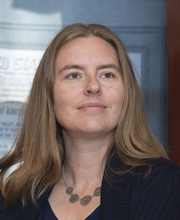
\includegraphics[width=1.04167in,height=\textheight]{assets/images/headshots/WARINNER_Christina.png}
& 🇺🇸 \textbf{Christina Warinner} is Group Leader of Microbiome Sciences
at the Max Planck Institute for Evolutionary Anthropology in Leipzig,
Germany, and Associate Professor of Anthropology at Harvard University.
She serves on the Leadership Team of the Max Planck-Harvard Research
Center for the Archaeoscience of the Ancient Mediterranean (MHAAM), and
is a Professor in the Faculty of Biological Sciences at Friedrich
Schiller University in Jena, Germany. Her research focuses on the use of
metagenomics and paleoproteomics to better understand past human diet,
health, and the evolution of the human microbiome. \\
2022 &
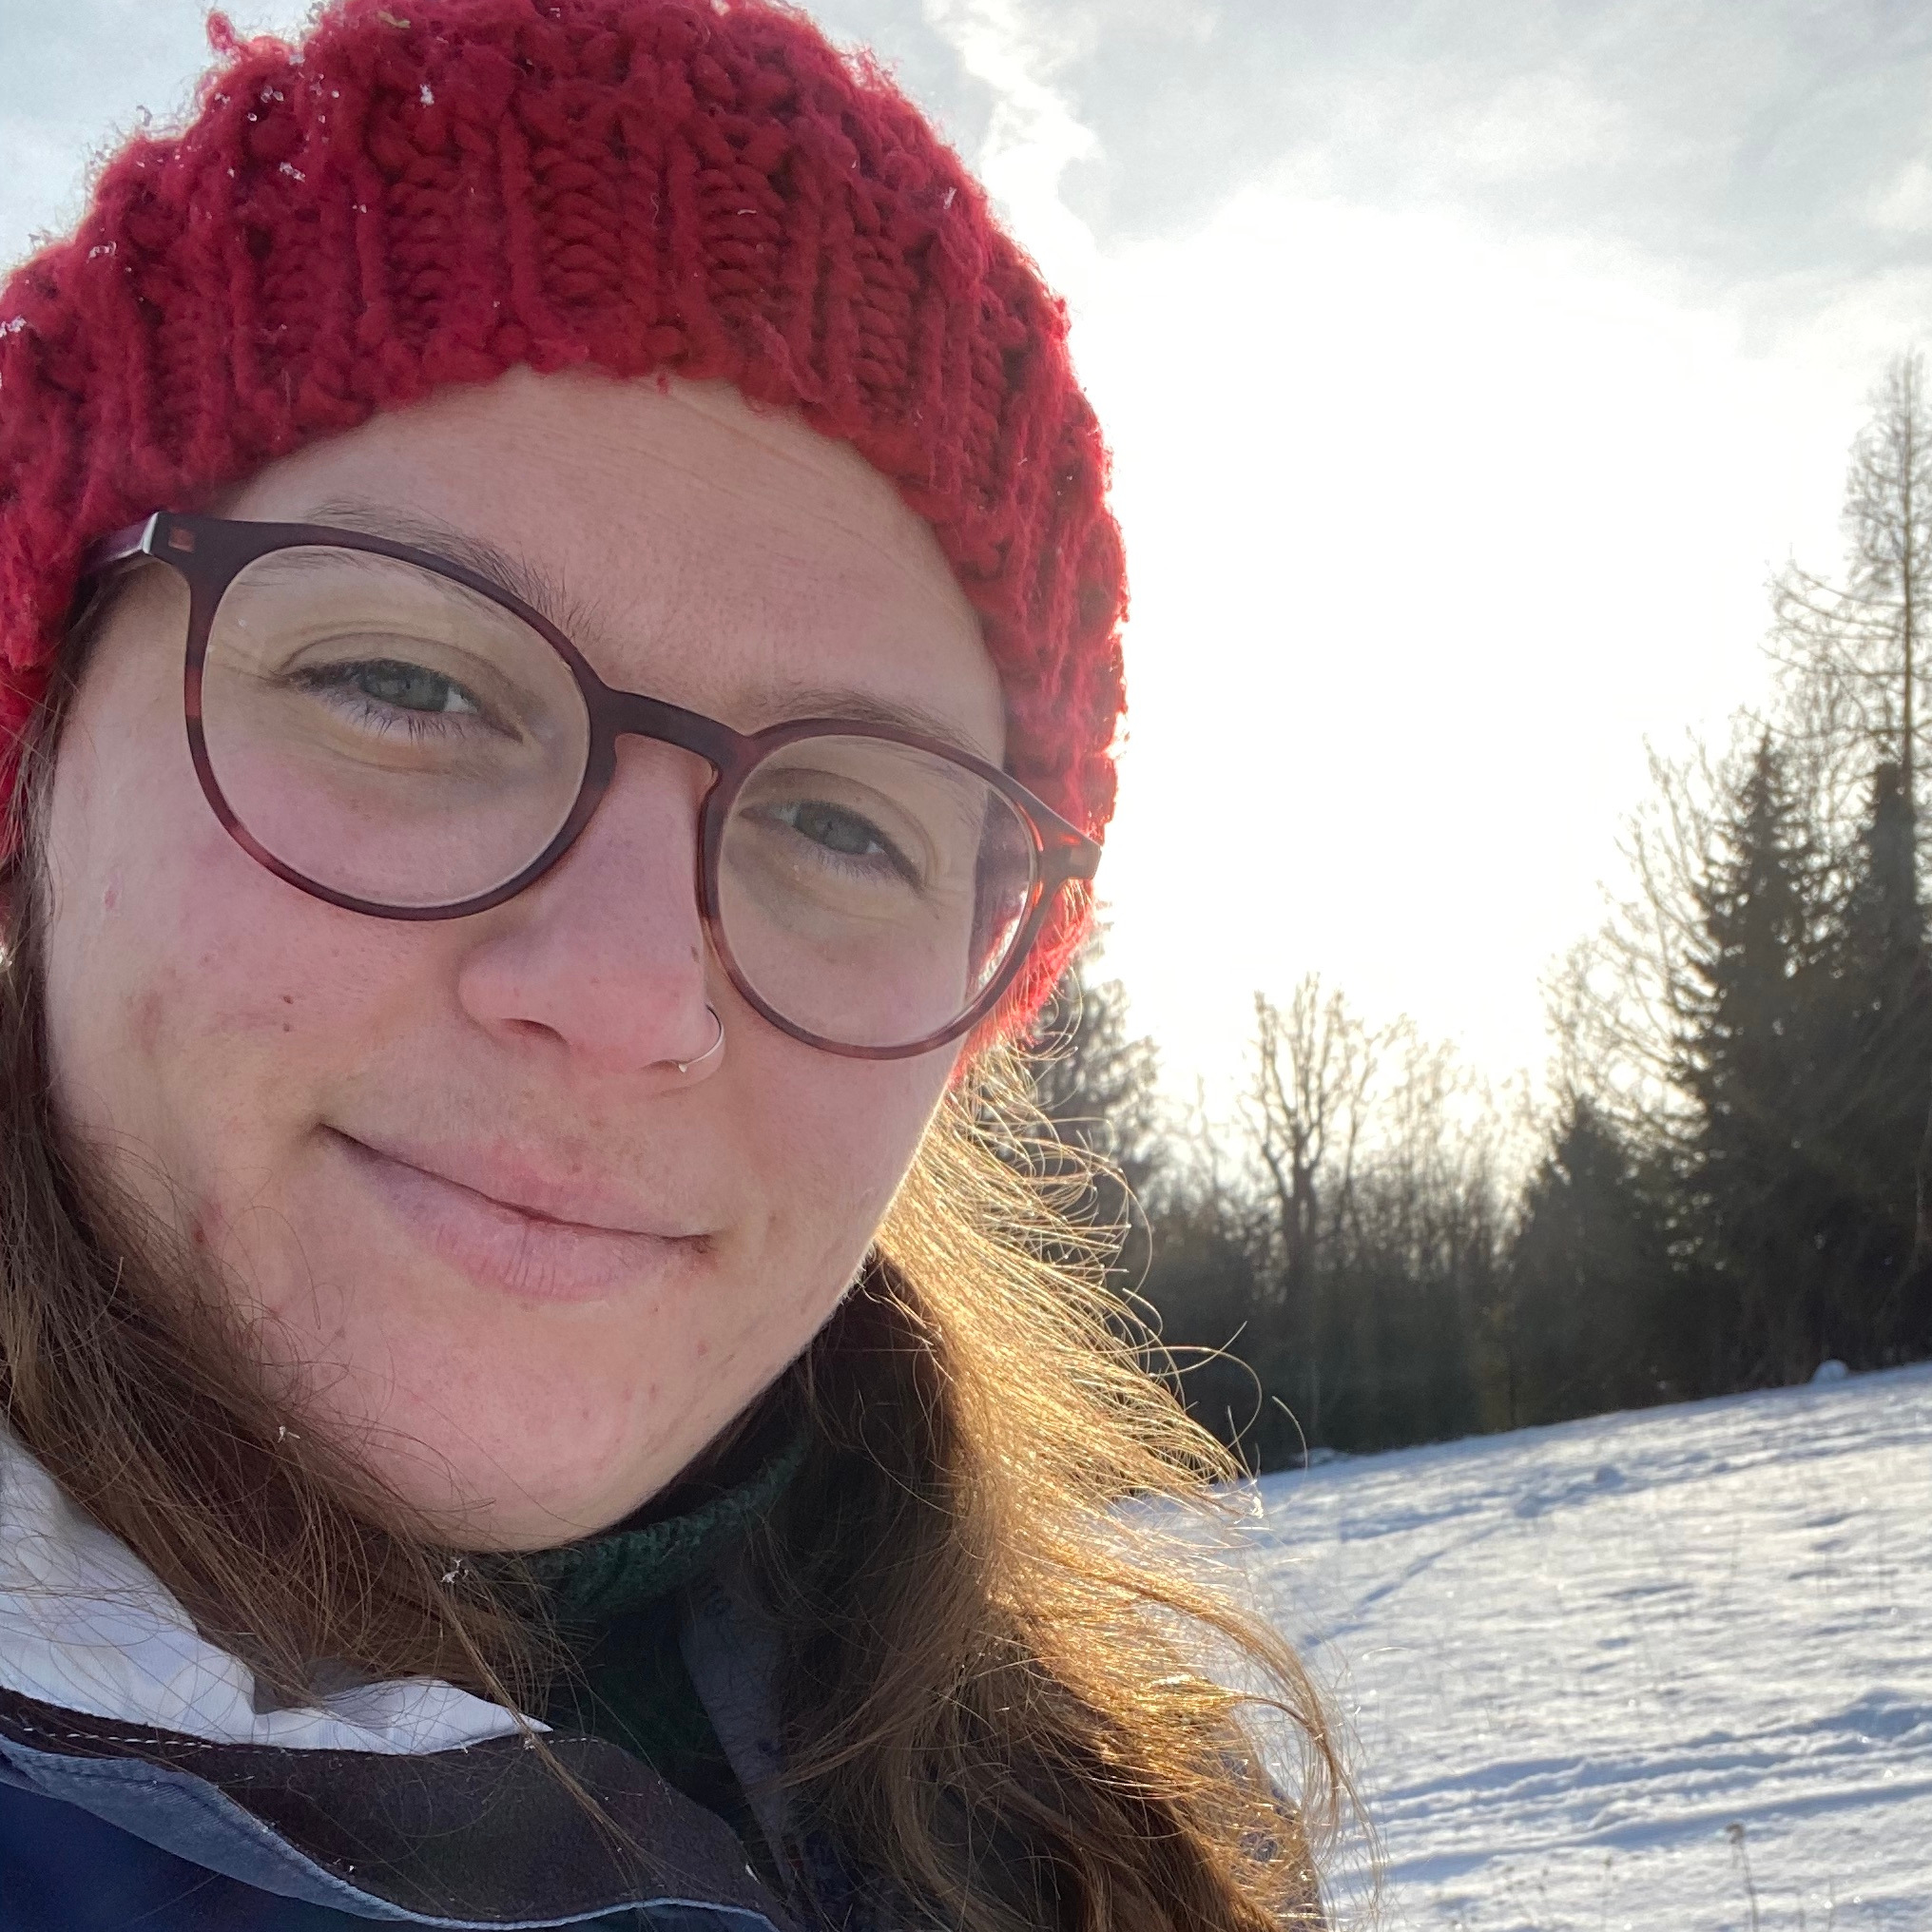
\includegraphics[width=1.04167in,height=\textheight]{assets/images/headshots/ANDRADES_VALTUENA_Aida.jpg}
& 🇪🇸 \textbf{Aida Andrades Valtueña} is a geneticist interested in
pathogen evolution, with particular interest in prehistoric pathogens.
She has been exploring new methods to analyse ancient pathogen data to
understand their past function and ecology to inform models of pathogen
emergence. \\
2022 &
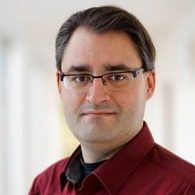
\includegraphics[width=1.04167in,height=\textheight]{assets/images/headshots/HERBIG_Alexander.jpeg}
& 🇩🇪 \textbf{Alexander Herbig} is a bioinformatician and group leader
for Computational Pathogenomics at the Max Planck Institute for
Evolutionary Anthropology. His main interest is in studying the
evolution of human pathogens and in methods development for pathogen
detection and bacterial genomics. \\
2022 &
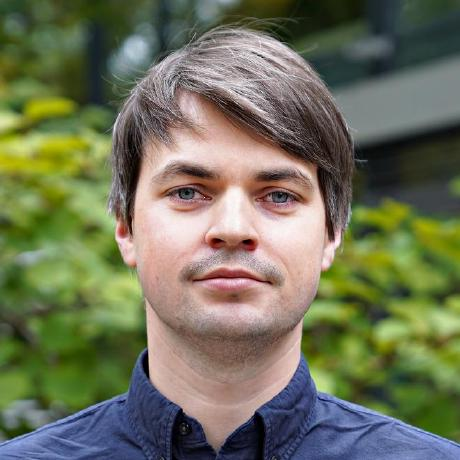
\includegraphics[width=1.04167in,height=\textheight]{assets/images/headshots/HUEBNER_Alex.jpg}
& 🇩🇪 \textbf{Alex Hübner} is a computational biologist, who originally
studied biotechnology, before switching to evolutionary biology during
his PhD. For his postdoc in the Warinner lab, he focuses on
investigating whether new methods in the field of modern metagenomics
can be directly applied to ancient DNA data. Here, he is particularly
interested in the \emph{de novo} assembly of ancient metagenomic
sequencing data and the subsequent analysis of its results. \\
2022 &
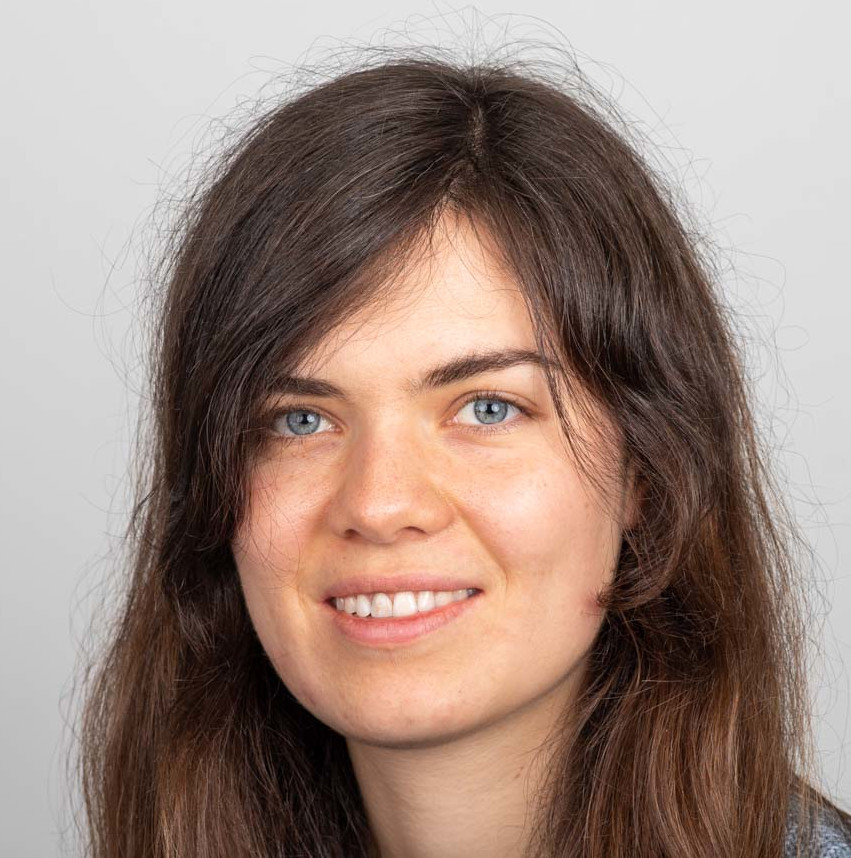
\includegraphics[width=1.04167in,height=\textheight]{assets/images/headshots/HISS_Alina.jpg}
& 🇩🇪 \textbf{Alina Hiss} is a PhD student in the Computational
Pathogenomics group at the Max Planck Institute for Evolutionary
Anthropology. She is interested in the evolution of human pathogens and
working on material from the Carpathian basin to gain insights about the
presence and spread of pathogens in the region during the Early Medieval
period. \\
2022 &
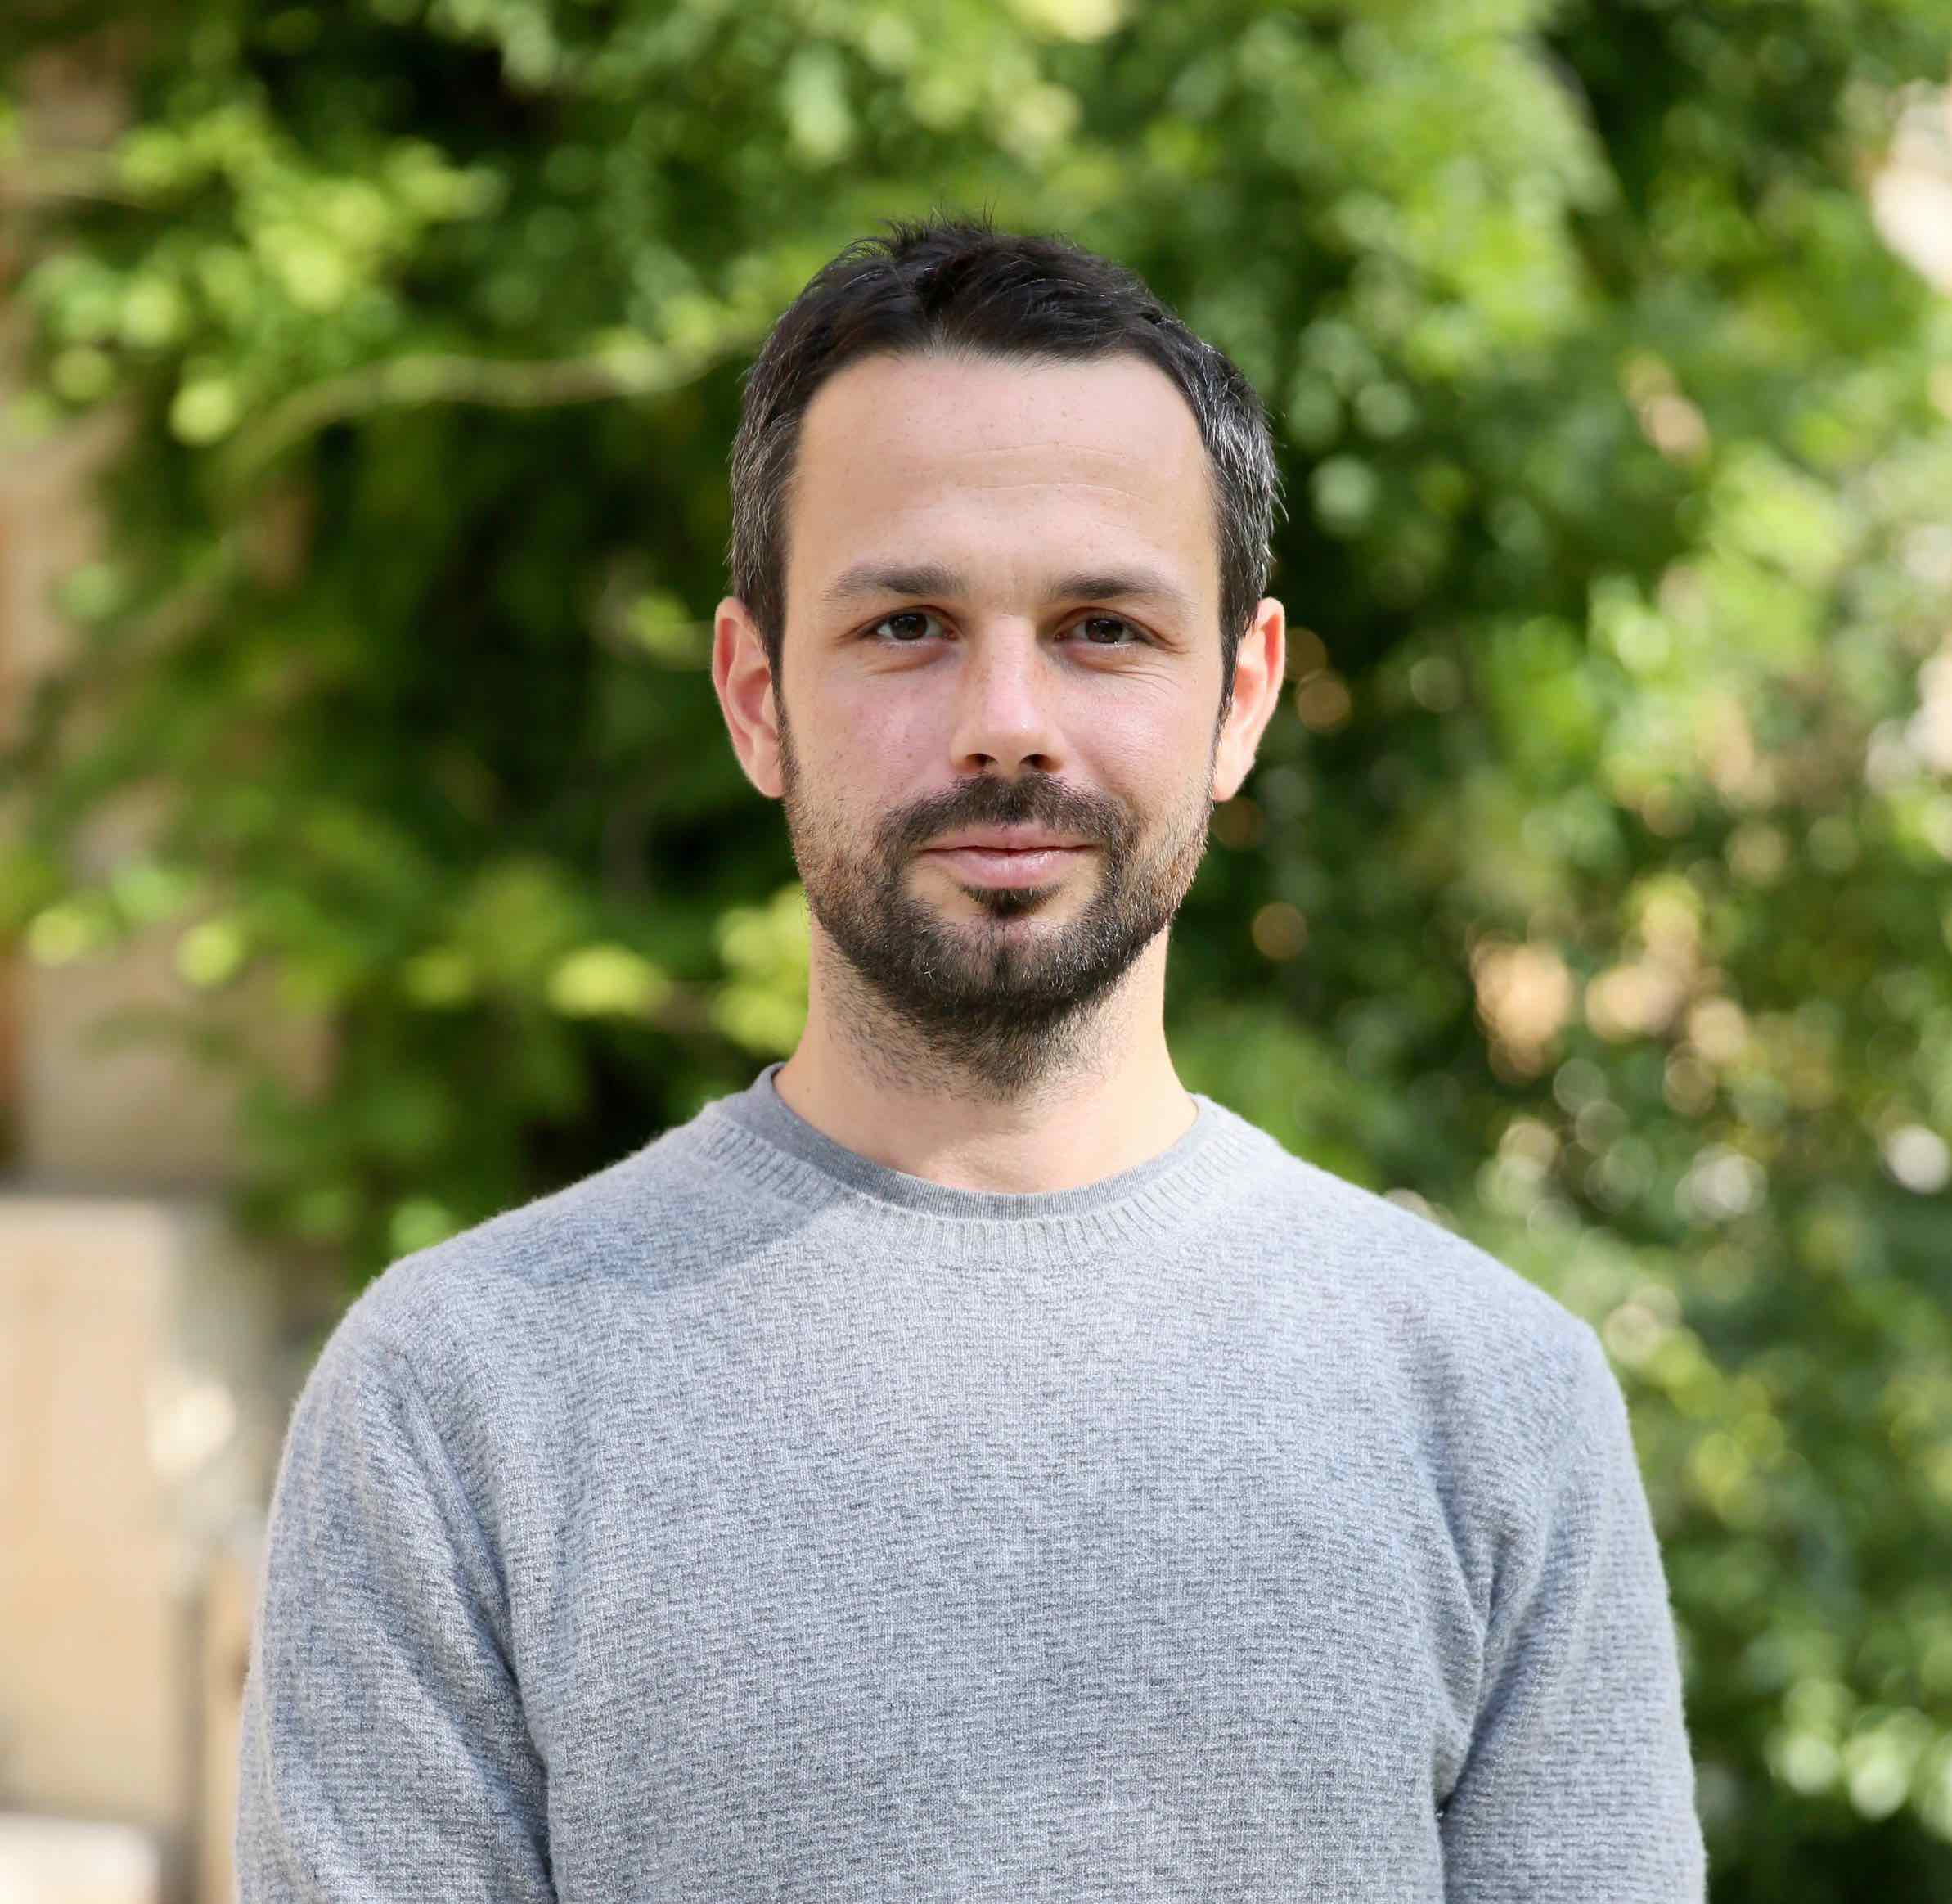
\includegraphics[width=1.04167in,height=\textheight]{assets/images/headshots/KOCHER_Arthur.jpg}
& 🇫🇷 \textbf{Arthur Kocher} initially trained as a veterinarian. He then
pursued a PhD in the field of disease ecology, during which he studied
the impact of biodiversity changes on the transmission of zoonotic
diseases using molecular tools such as DNA metabarcoding. During his
Post-Docs, he extended his research focus to evolutionary aspects of
pathogens, which he currently investigates using ancient genomic data
and Bayesian phylogenetics. \\
2022 &
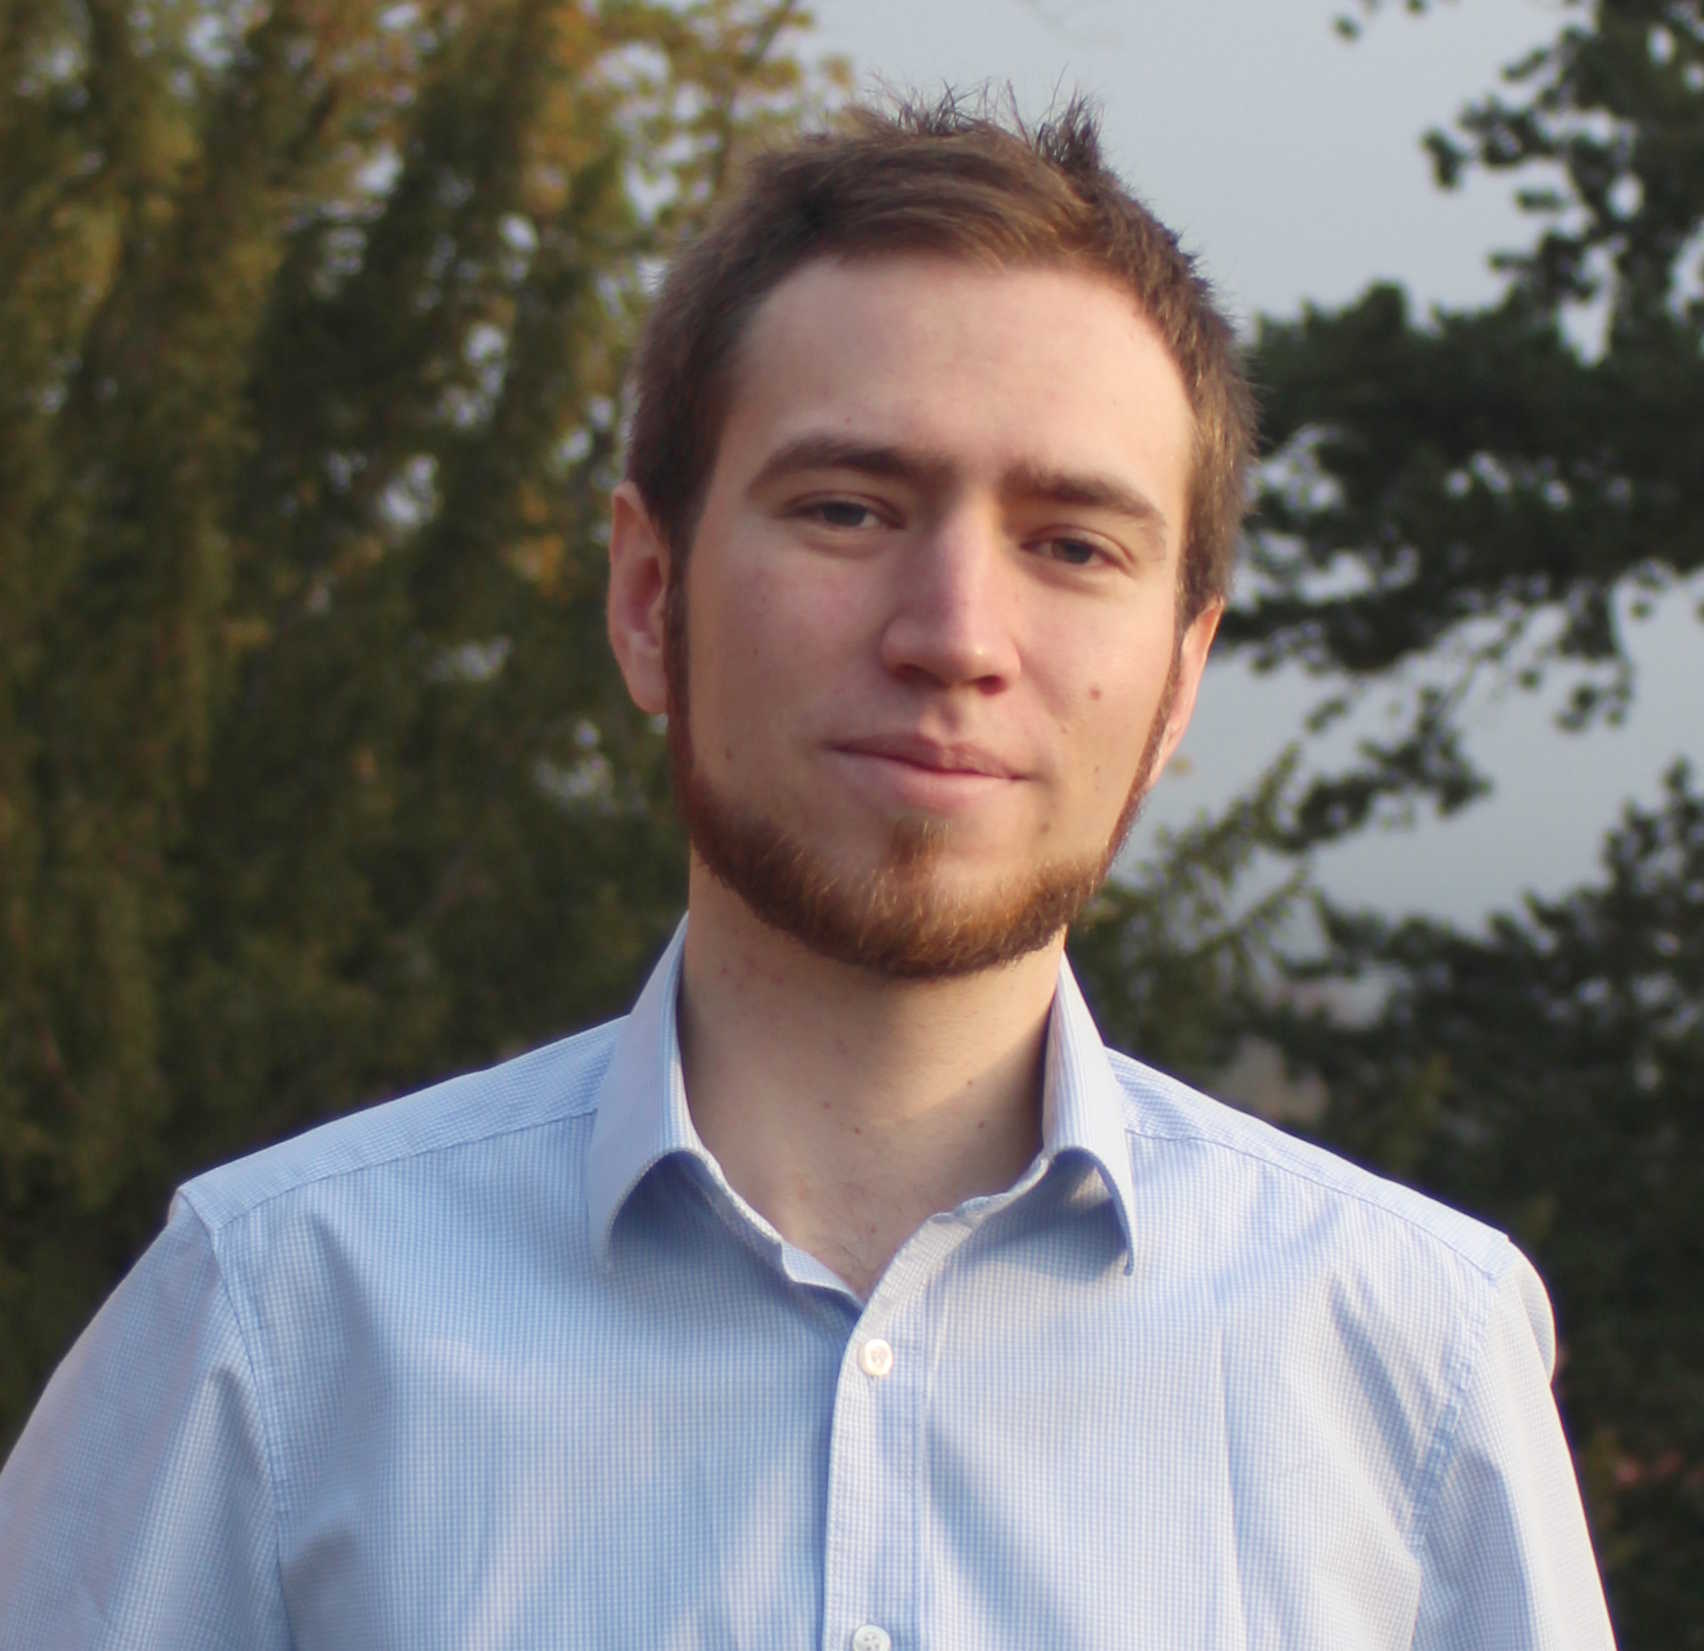
\includegraphics[width=1.04167in,height=\textheight]{assets/images/headshots/SCHMID_Clemens.JPG}
& 🇩🇪 \textbf{Clemens Schmid} is a computational archaeologist pursuing a
PhD in the group of Stephan Schiffels at the department of
Archaeogenetics at the Max Planck Institute for Evolutionary
Anthropology. He is trained both in archaeology and computer science and
currently develops computational methods for the spatiotemporal
co-analysis of archaeological and ancient genomic data. He worked in
research projects on the European Neolithic, Copper and Bronze age and
maintains research software in R, C++ and Haskell. \\
2022 &
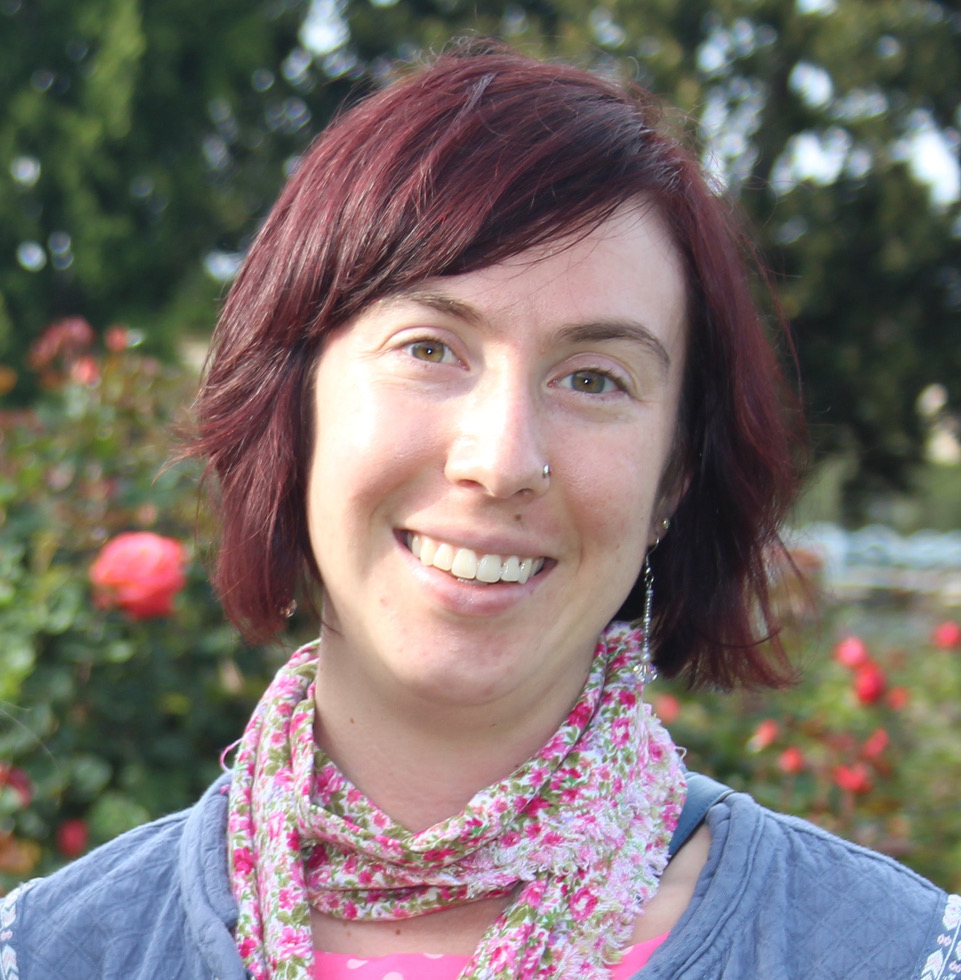
\includegraphics[width=1.04167in,height=\textheight]{assets/images/headshots/VELSKO_Irina.jpeg}
& 🇺🇸 \textbf{Irina Velsko} is a postdoc in the Microbiome group of the
department of Archaeogenetics at the Max Planck Institute for
Evolutionary Anthropology. She did her PhD work on oral microbiology and
immunology of the living, and now works on oral microbiomes of the
living and the dead. Her work focuses on the evolution and ecology of
dental plaque biofilms, both modern and ancient, and the complex
interplay between microbiomes and their hosts. \\
2022 &

\includegraphics[width=1.04167in,height=\textheight]{assets/images/headshots/BORRY_Maxime.png}
& 🇫🇷 \textbf{Maxime Borry} is a doctoral researcher in bioinformatics at
the Max Planck Institute for Evolutionary Anthropology in Germany. After
an undergraduate in life sciences and a master in Ecology, followed by a
master in bioinformatics, he is now working on the completion of his
PhD, focused on developing new tools and data analysis of ancient
metagenomic samples. \\
2022 &
\includegraphics[width=1.04167in,height=\textheight]{assets/images/headshots/MICHEL_Megan.jpg}
& 🇺🇸 \textbf{Megan Michel} is a PhD student jointly affiliated with the
Archaeogenetics Department at the Max Planck Institute for Evolutionary
Anthropology and the Human Evolutionary Biology Department at Harvard
University. Her research focuses on using computational genomic analyses
to understand how pathogens have co-evolved with their hosts over the
course of human history. \\
2022 &
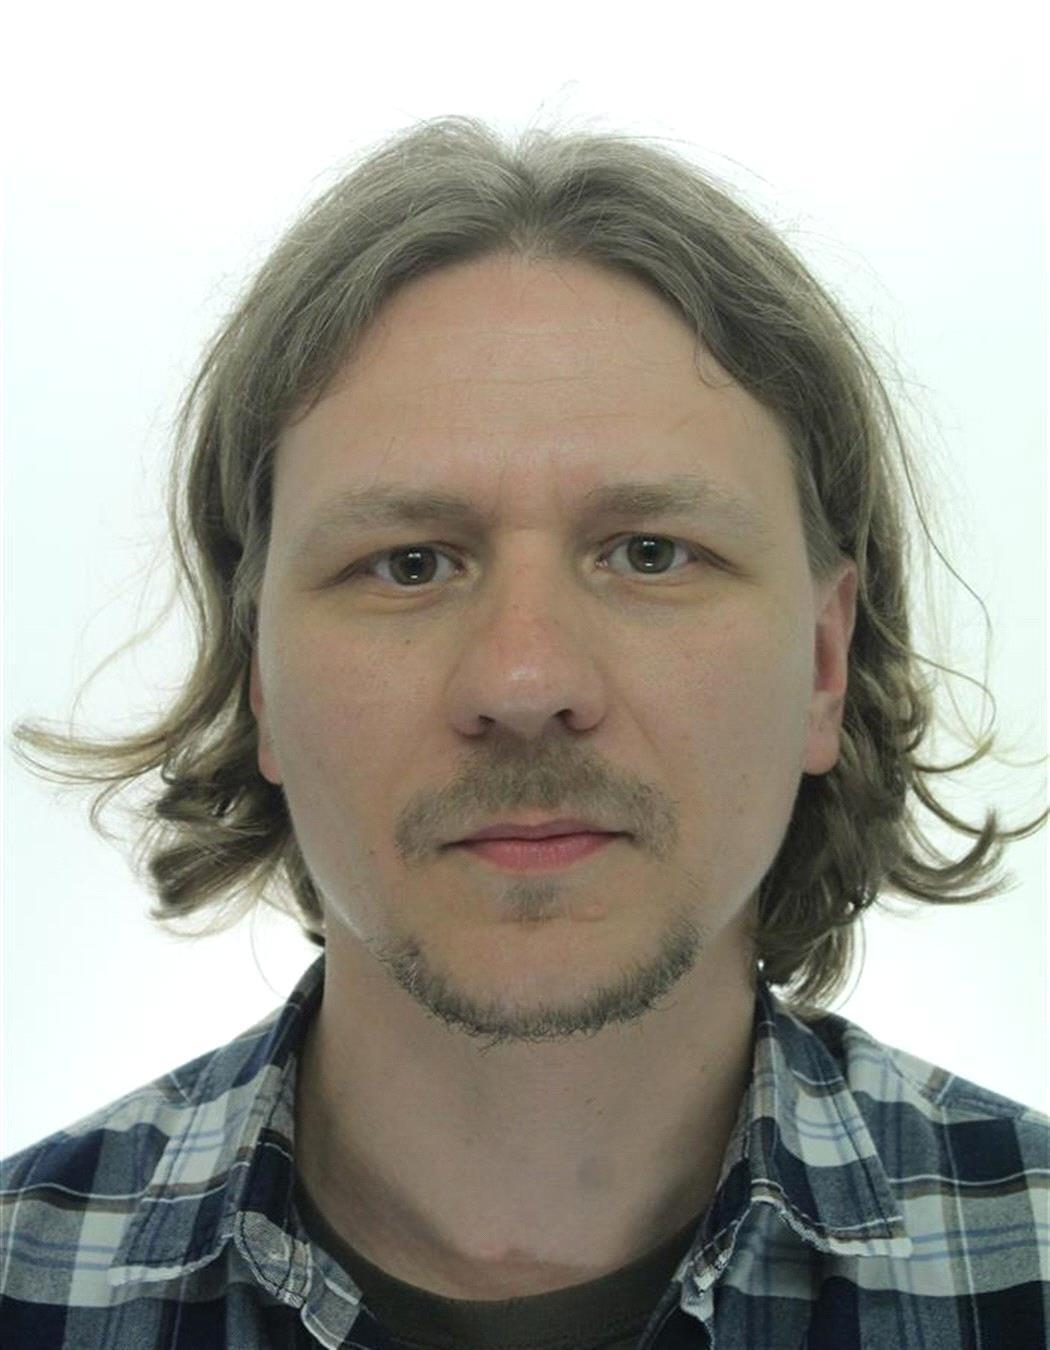
\includegraphics[width=1.04167in,height=\textheight]{assets/images/headshots/OSKOLKOV_Nikolay.jpg}
& 🇷🇺 \textbf{Nikolay Oskolkov} is a bioinformatician at Lund University
and the bioinformatics platform of SciLifeLab, Sweden. He defended his
PhD in theoretical physics in 2007, and switched to life sciences in
2012. His research interests include mathematical statistics and machine
learning applied to genetics and genomics, single cell and ancient
metagenomics data analysis. \\
2022 &

\includegraphics[width=1.04167in,height=\textheight]{assets/images/headshots/DUCHENE_Sebastian.jpeg}
& 🇦🇺 \textbf{Sebastian Duchene} is an Australian Research Council Fellow
at the Doherty Institute for Infection and Immunity at the University of
Melbourne, Australia. Prior to joining the University of Melbourne he
obtained his PhD and conducted postdoctoral work at the University of
Sydney. His research is in molecular evolution and epidemiology of
infectious pathogens, notably viruses and bacteria, and developing
Bayesian phylodynamic methods. \\
2022 &

\includegraphics[width=1.04167in,height=\textheight]{assets/images/headshots/LAMNIDIS_Thiseas.jpg}
& 🇬🇷 \textbf{Thiseas Lamnidis} is a human population geneticist
interested in European population history after the Bronze Age. To gain
the required resolution to differentiate between Iron Age European
populations, he is developing analytical methods based on the sharing of
rare variation between individuals. He has also contributed to pipelines
that streamline the processing and analysis of genetic data in a
reproducible manner, while also facilitating dissemination of
information among interdisciplinary colleagues. \\
\end{longtable}

\bookmarksetup{startatroot}

\hypertarget{acknowledgements}{%
\chapter*{Acknowledgements}\label{acknowledgements}}
\addcontentsline{toc}{chapter}{Acknowledgements}

\markboth{Acknowledgements}{Acknowledgements}

We would like to thank the following supporters of the original summer
schools and eventual textbook.

\hypertarget{financial-support}{%
\section*{\texorpdfstring{\textbf{Financial
Support}}{Financial Support}}\label{financial-support}}
\addcontentsline{toc}{section}{\textbf{Financial Support}}

\markright{\textbf{Financial Support}}


\includegraphics[width=2.08333in,height=\textheight]{assets/images/logos/WSS_Logo_16mm_600_rgb.png}

The content of this textbook was developed from the SPAAM Summer School:
Introduction to Ancient Metagenomics summer school series, sponsored by
the Werner Siemens-Stiftung (Grant: Paleobiotechnology, awarded to
Pierre Stallforth, Hans-Knöll Institute, and Christina Warinner, Max
Planck Institute for Evolutionary Anthropology)

\hypertarget{institutional-support}{%
\section*{\texorpdfstring{\textbf{Institutional
Support}}{Institutional Support}}\label{institutional-support}}
\addcontentsline{toc}{section}{\textbf{Institutional Support}}

\markright{\textbf{Institutional Support}}

\begin{figure}

\begin{minipage}[t]{0.20\linewidth}

{\centering 

\raisebox{-\height}{


\includegraphics[width=2.08333in,height=\textheight]{assets/images/logos/leibniz_hki.png}

}

}

\end{minipage}%
%
\begin{minipage}[t]{0.20\linewidth}

{\centering 

\raisebox{-\height}{


\includegraphics[width=2.08333in,height=\textheight]{assets/images/logos/mhaam.png}

}

}

\end{minipage}%
%
\begin{minipage}[t]{0.40\linewidth}

{\centering 

\raisebox{-\height}{


\includegraphics[width=4.16667in,height=\textheight]{assets/images/logos/MPI_Logo_DE_CMYK_green.png}

}

}

\end{minipage}%
%
\begin{minipage}[t]{0.20\linewidth}

{\centering 

\raisebox{-\height}{


\includegraphics[width=2.08333in,height=\textheight]{assets/images/logos/JSMC Logo.png}

}

}

\end{minipage}%

\end{figure}

\hypertarget{infrastructural-support}{%
\section*{\texorpdfstring{\textbf{Infrastructural
Support}}{Infrastructural Support}}\label{infrastructural-support}}
\addcontentsline{toc}{section}{\textbf{Infrastructural Support}}

\markright{\textbf{Infrastructural Support}}


\includegraphics[width=2.08333in,height=\textheight]{index_files/mediabag/assets/images/logos/denbi-logo-color.pdf}

The practical sessions of the summers schools work was supported by the
BMBF-funded de.NBI Cloud within the German Network for Bioinformatics
Infrastructure (de.NBI) (031A532B, 031A533A, 031A533B, 031A534A,
031A535A, 031A537A, 031A537B, 031A537C, 031A537D, 031A538A). z

\bookmarksetup{startatroot}

\hypertarget{before-you-start}{%
\chapter*{Before you Start}\label{before-you-start}}
\addcontentsline{toc}{chapter}{Before you Start}

\markboth{Before you Start}{Before you Start}

The summer school course that this textbook is derived from was designed
to be as practical as possible. This means that most of the chapters are
designed to act as a walkthrough to guide you through the steps on how
to generate and analyse data for each of the major steps of an ancient
metagenomics project.

The summer school utilised cloud computing to provide a consistent
computing platform for all participants, however all tools and data
demonstrated are open-source and publicly available.

\begin{tcolorbox}[enhanced jigsaw, opacitybacktitle=0.6, bottomtitle=1mm, opacityback=0, colback=white, coltitle=black, leftrule=.75mm, toprule=.15mm, title=\textcolor{quarto-callout-warning-color}{\faExclamationTriangle}\hspace{0.5em}{Warning}, colframe=quarto-callout-warning-color-frame, toptitle=1mm, arc=.35mm, left=2mm, titlerule=0mm, breakable, rightrule=.15mm, bottomrule=.15mm, colbacktitle=quarto-callout-warning-color!10!white]

Bioinformatics often involve large computing resource requirements!
While we aim to make example data and processing as efficient as
possible, we cannot guarantee that they will all be able to work on
standard laptops or desktop computing - most likely due to memory/RAM
requirements. As a guide, the cloud nodes used during the summer school
had 16 cores and 32 GB of RAM.

\end{tcolorbox}

To following the practical chapters of this text book, you will require:

\begin{itemize}
\tightlist
\item
  A unix based operating system (e.g., Linux, MacOS, or possibly Windows
  with Linux Subsystem - however the latter has not be tested )
\item
  A corresponding Unix terminal
\item
  An internet connection
\item
  A web browser
\item
  A
  \href{https://docs.conda.io/en/latest/miniconda.html}{\texttt{conda}}
  installation with
  \href{https://bioconda.github.io/\#usage}{\texttt{bioconda}}
  configured.

  \begin{itemize}
  \tightlist
  \item
    Conda is a very popular package manager for installing software in
    bioinformatics. \texttt{bioconda} is a the main source of
    bioinformatics software for conda.
  \item
    To speed up installation, we would also highly recommend setting up
    the
    \href{https://www.anaconda.com/blog/a-faster-conda-for-a-growing-community}{\texttt{libmamba-solver}}
  \end{itemize}
\end{itemize}

For each chapter we will provide a link to a \texttt{tar} archive that
will contain the raw data and a conda \texttt{yml} file that specifies
the software environment for that chapter.

Before loading the environment for the exercises, the environment will
need to be installed using the \texttt{yml} with the instructions below,
and then activated. A list of the software in each chapter's environment
can be found in the \protect\hyperlink{conda-environments}{Appendix}.

\hypertarget{creating-a-conda-environment}{%
\section*{Creating a conda
environment}\label{creating-a-conda-environment}}
\addcontentsline{toc}{section}{Creating a conda environment}

\markright{Creating a conda environment}

Once \texttt{conda} is installed and \texttt{bioconda} configured, at
the beginning of each chapter, to create the \texttt{conda} environment
from the \texttt{yml} file, you will need to run the following:

\begin{enumerate}
\def\labelenumi{\arabic{enumi}.}
\item
  Download the Zenodo tar archive file either the download button and or
  `Copy link address' the URL and run

\begin{Shaded}
\begin{Highlighting}[]
\ExtensionTok{curl} \AttributeTok{{-}O} \OperatorTok{\textless{}}\NormalTok{url}\OperatorTok{\textgreater{}}
\CommentTok{\#\# or}
\FunctionTok{wget} \OperatorTok{\textless{}}\NormalTok{url}\OperatorTok{\textgreater{}}
\end{Highlighting}
\end{Shaded}
\item
  Extract the tar archive with

\begin{Shaded}
\begin{Highlighting}[]
\FunctionTok{tar} \AttributeTok{{-}xvf} \OperatorTok{\textless{}}\NormalTok{tar\_file}\OperatorTok{\textgreater{}}\NormalTok{.tar.gz}
\end{Highlighting}
\end{Shaded}

  and change into the directory with

\begin{Shaded}
\begin{Highlighting}[]
\BuiltInTok{cd} \OperatorTok{\textless{}}\NormalTok{directory}\OperatorTok{\textgreater{}}\NormalTok{/}
\end{Highlighting}
\end{Shaded}
\item
  Within the resulting directory run the following conda command to
  install the software into it's dedicated environment

\begin{Shaded}
\begin{Highlighting}[]
\ExtensionTok{conda}\NormalTok{ env create }\AttributeTok{{-}f} \OperatorTok{\textless{}}\NormalTok{env\_file}\OperatorTok{\textgreater{}}\NormalTok{.yml}
\end{Highlighting}
\end{Shaded}

  ::: \{.callout-note\} Note: you only have to run the environment
  creation once. :::
\item
  Follow the instructions as prompted. Once created, you can see a list
  of environments with

\begin{Shaded}
\begin{Highlighting}[]
\ExtensionTok{conda}\NormalTok{ env list}
\end{Highlighting}
\end{Shaded}
\item
  To load the relevant environment, you can run

\begin{Shaded}
\begin{Highlighting}[]
\ExtensionTok{conda}\NormalTok{ activate }\OperatorTok{\textless{}}\NormalTok{name\_of\_envonment}\OperatorTok{\textgreater{}}\NormalTok{.yml}
\end{Highlighting}
\end{Shaded}
\item
  Once finished with the chapter, you can deactivate the environment
  with

\begin{Shaded}
\begin{Highlighting}[]
\ExtensionTok{conda}\NormalTok{ deactivate}
\end{Highlighting}
\end{Shaded}
\end{enumerate}

To reuse the environment, just run step 4 and 5 as necessary.

\begin{tcolorbox}[enhanced jigsaw, opacitybacktitle=0.6, bottomtitle=1mm, opacityback=0, colback=white, coltitle=black, leftrule=.75mm, toprule=.15mm, title=\textcolor{quarto-callout-tip-color}{\faLightbulb}\hspace{0.5em}{Tip}, colframe=quarto-callout-tip-color-frame, toptitle=1mm, arc=.35mm, left=2mm, titlerule=0mm, breakable, rightrule=.15mm, bottomrule=.15mm, colbacktitle=quarto-callout-tip-color!10!white]

To delete a conda software environment, just get the path listed on
\texttt{conda\ env\ list} and delete the folder with
\texttt{rm\ -rf\ \textless{}path\textgreater{}}.

\end{tcolorbox}

\hypertarget{additional-software-.}{%
\section*{Additional Software .}\label{additional-software-.}}
\addcontentsline{toc}{section}{Additional Software .}

\markright{Additional Software .}

For some chapters you may need the following software/and or data
manually installed, which are not available on \texttt{bioconda}:

\begin{itemize}
\tightlist
\item
  \emph{De novo} assembly

  \begin{itemize}
  \tightlist
  \item
    MetaWrap
  \end{itemize}

\begin{Shaded}
\begin{Highlighting}[]
\ExtensionTok{conda}\NormalTok{ create }\AttributeTok{{-}n}\NormalTok{ metawrap{-}env python=2.7}
\ExtensionTok{conda}\NormalTok{ activate metawrap{-}env}
\ExtensionTok{conda}\NormalTok{ install biopython bwa maxbin2 metabat2 samtools=1.9}
\BuiltInTok{cd}\NormalTok{ \textasciitilde{}/bin/}
\FunctionTok{git}\NormalTok{ clone https://github.com/bxlab/metaWRAP.git}
\BuiltInTok{echo} \StringTok{"export PATH=}\VariableTok{$PATH}\StringTok{:\textasciitilde{}/bin/metaWRAP/bin"} \OperatorTok{\textgreater{}\textgreater{}}\NormalTok{ \textasciitilde{}/.bashrc}
\end{Highlighting}
\end{Shaded}
\item
  Functional Profiling

  \begin{itemize}
  \item
    HUMAnN3 UniRef database (where the functional providing conda
    environment is already activated - see the Functional Profiling
    chapter for more details)

\begin{Shaded}
\begin{Highlighting}[]
\ExtensionTok{humann3\_databases} \AttributeTok{{-}{-}download}\NormalTok{ uniref uniref90\_ec\_filtered\_diamond /vol/volume/5c{-}functional{-}genomics/humann3\_db}
\end{Highlighting}
\end{Shaded}
  \end{itemize}
\item
  Phylogenomics

  \begin{itemize}
  \item
    \href{http://tree.bio.ed.ac.uk/download.html?name=tempest\&id=102\&num=3}{Tempest}
    (v1.5.3)
  \item
    It is also recommended to assign the following \texttt{bash}
    variable so you can access the tool without the full path

\begin{Shaded}
\begin{Highlighting}[]
\BuiltInTok{export} \VariableTok{tempest}\OperatorTok{=}\StringTok{\textquotesingle{}bash /home/ubuntu/bin/TempEst\_v1.5.3/bin/tempest\textquotesingle{}}
\end{Highlighting}
\end{Shaded}
  \item
    \href{https://www.megasoftware.net}{MEGAX} (v11.0.11)
  \end{itemize}
\end{itemize}

\part{Theory}

In the first section of this book we will introduce the basic concepts
of a range of topics related to ancient DNA, from how Next Generation
Sequencing (NGS) sequencing works, to the fundamental biochemistry of
ancient DNA, to the phylogenomic analysis of reconstructed genomes.

The content of this section of the book were originally delivered as
lectures, and each chapter will have a recording of the lectures and the
accompanying slides.

\hypertarget{lectures}{%
\section*{Lectures}\label{lectures}}
\addcontentsline{toc}{section}{Lectures}

\markright{Lectures}

\hypertarget{introduction-to-ngs-sequencing}{%
\subsection*{\texorpdfstring{\protect\hyperlink{introduction-to-ngs-sequencing-1}{Introduction
to NGS
Sequencing}}{Introduction to NGS Sequencing}}\label{introduction-to-ngs-sequencing}}
\addcontentsline{toc}{subsection}{\protect\hyperlink{introduction-to-ngs-sequencing-1}{Introduction
to NGS Sequencing}}

In this chapter, we will introduce how we are able to convert DNA
molecules to human readable sequences of A, C, T, and Gs, which we can
subsequently can computationally analyse.

The field of Ancient DNA was revolutionised by the development of `Next
Generation Sequencing' (NGS), which relies on sequencing of millions of
\emph{short} fragments of DNA in parallel. The global leading DNA
sequencing company is Illumina, and the technology used by Illumina is
also most popular by palaeogeneticists. Therefore we will go through the
various technologies behind Illumina next-generation sequencing
machines.

We will also look at some important differences in the way different
models of Illumina sequences work, and how this can influence ancient
DNA research. Finally we will cover the structure of `FASTQ' files, the
most popular file format for representing the DNA sequence output of NGS
sequencing machines.

\hypertarget{introduction-to-ancient-dna}{%
\subsection*{\texorpdfstring{\protect\hyperlink{introduction-to-ancient-dna-1}{Introduction
to Ancient
DNA}}{Introduction to Ancient DNA}}\label{introduction-to-ancient-dna}}
\addcontentsline{toc}{subsection}{\protect\hyperlink{introduction-to-ancient-dna-1}{Introduction
to Ancient DNA}}

This chapter introduces you to ancient DNA and the enormous
technological changes that have taken place since the field's origins in
1984. Starting with the quagga and proceeding to microbes, we discuss
where ancient microbial DNA can be found in the archaeological record
and examine how ancient DNA is defined by its condition, not by a fixed
age.

We next cover genome basics and take an in-depth look at the way DNA
degrades over time. We detail the fundamentals of DNA damage, including
the specific chemical processes that lead to DNA fragmentation and
C-\textgreater T miscoding lesions. We then demystify the DNA damage
``smiley plot'' and explain the how the plot's symmetry or asymmetry is
related to the specific enzymes used to repair DNA during library
construction. We discuss how DNA damage is and is not clock-like, how to
interpret and troubleshoot DNA damage plots, and how DNA damage patters
can be used to authenticate ancient samples, specific taxa, and even
sequences. We cover laboratory strategies for removing or reducing
damage for greater accuracy for genotype calling, and we discuss the
pros and cons of single-stranded library protocols. We then take a
closer look at proofreading and non-proofreading polymerases and note
key steps in NGS library preparation during which enzyme selection is
critical in ancient DNA studies.

Finally, we examine the big picture of why DNA damage matters in ancient
microbial studies, and its effects on taxonomic identification of
sequences, accurate genome mapping, and metagenomic assembly.

\hypertarget{introduction-to-metagenomics}{%
\subsection*{\texorpdfstring{\protect\hyperlink{introduction-to-metagenomics-1}{Introduction
to
Metagenomics}}{Introduction to Metagenomics}}\label{introduction-to-metagenomics}}
\addcontentsline{toc}{subsection}{\protect\hyperlink{introduction-to-metagenomics-1}{Introduction
to Metagenomics}}

This chapter introduces you to the basics of metagenomics, with an
emphasis on tools and approaches that are used to study ancient
metagenomes. We begin by covering the basic terminology used in
metagenomics and microbiome research and discuss how the field has
changed over time. We examine the species concept for microbes and
challenges that arise in classifying microbial species with respect to
taxonomy and phylogeny. We then proceed to taxonomic profiling and
discuss the pros and cons of different taxonomic profilers.

Afterwards, we explain how to estimate preservation in ancient
metagenomic samples and how to clean up your datasets and remove
contaminants. Finally, we discuss strategies for exploring and comparing
the ecological diversity in your samples, including different strategies
for data normalization, distance calculation, and ordination.

\hypertarget{introduction-to-microbial-genomics}{%
\subsection*{\texorpdfstring{\protect\hyperlink{introduction-to-microbial-genomics-1}{Introduction
to Microbial
Genomics}}{Introduction to Microbial Genomics}}\label{introduction-to-microbial-genomics}}
\addcontentsline{toc}{subsection}{\protect\hyperlink{introduction-to-microbial-genomics-1}{Introduction
to Microbial Genomics}}

The field of microbial genomics aims at the reconstruction and
comparative analyses of genomes for gaining insights into the genetic
foundation and evolution of various functional aspects such as virulence
mechanisms in pathogens.

Including data from ancient samples into this comparative assessment
allows for studying these evolutionary changes through time. This, for
example, provides insights into the emergence of human pathogens and
their development in conjunction with human cultural transitions.

In this chapter we will look examples for how to utilise data from
ancient genomes in comparative studies of human pathogens and today's
practical sessions will highlight methodologies for the reconstruction
of microbial genomes.

\hypertarget{introduction-to-evolutionary-biology}{%
\subsection*{\texorpdfstring{\protect\hyperlink{introduction-to-evolutionary-biology-1}{Introduction
to Evolutionary
Biology}}{Introduction to Evolutionary Biology}}\label{introduction-to-evolutionary-biology}}
\addcontentsline{toc}{subsection}{\protect\hyperlink{introduction-to-evolutionary-biology-1}{Introduction
to Evolutionary Biology}}

Pathogen genome data are an invaluable source of information about the
evolution and spread of these organisms. This chapter will focus on
molecular phylogenetic methods and the insight that they can reveal from
improving our understanding of ancient evolution to the epidemiological
dynamics of current outbreaks.

The first section will introduce phylognenetic trees and a set of core
terms and concepts for their interpretation. Next, it will focus on some
of the most popular approaches to inferring phylogenetic trees; those
based on genetic distance, maximum likelihood, and Bayesian inference.
These methods carry important considerations regarding the process that
generated the data, computational capability, and data quality, all of
which will be discussed here. Finally, we will direct our attention to
examples of analyses of ancient and modern pathogens (e.g.~Yersinia
pestis, Hepatitis B virus, SARS-CoV-2) and critically assess appropriate
choice of models and methods.

\hypertarget{introduction-to-ngs-sequencing-1}{%
\chapter{Introduction to NGS
Sequencing}\label{introduction-to-ngs-sequencing-1}}

\hypertarget{lecture}{%
\section{Lecture}\label{lecture}}

PDF version of the slide lectures can be downloaded from
\href{https://raw.githubusercontent.com/SPAAM-community/wss-summer-school/main/docs/assets/slides/2022/1a-intro-to-ngs/SPAAM\%20Summer\%20School\%202022\%20-\%201A\%20-\%20Introduction\%20to\%20NGS\%20Data.pdf}{here}.

\hypertarget{readings}{%
\section{Readings}\label{readings}}

\hypertarget{reviews}{%
\subsection{Reviews}\label{reviews}}

(Schuster 2008)

(Shendure and Ji 2008)

(Slatko, Gardner, and Ausubel 2018)

(Dijk et al. 2014)

\hypertarget{sequencing-library-construction}{%
\subsection{Sequencing Library
Construction}\label{sequencing-library-construction}}

(Kircher, Sawyer, and Meyer 2012)

(Meyer and Kircher 2010)

\hypertarget{errors-and-considerations}{%
\subsection{Errors and Considerations}\label{errors-and-considerations}}

(Ma et al. 2019)

(Sinha et al. 2017)

(Valk et al. 2019)

\hypertarget{questions-to-think-about}{%
\section{Questions to think about}\label{questions-to-think-about}}

\begin{itemize}
\tightlist
\item
  Why is Illumina sequencing technologies useful for aDNA?
\item
  What problems can the 2-colour chemistry technology of NextSeq and
  NovaSeqs cause in downstream analysis?
\item
  Why is `Index-Hopping' a problem?
\item
  What is good software to evaluate the quality of your sequencing runs?
\end{itemize}

\hypertarget{introduction-to-ancient-dna-1}{%
\chapter{Introduction to Ancient
DNA}\label{introduction-to-ancient-dna-1}}

\hypertarget{lecture-1}{%
\section{Lecture}\label{lecture-1}}

PDF version of these slides can be downloaded from
\href{https://github.com/SPAAM-community/wss-summer-school/raw/main/docs/assets/slides/2022/2a-intro-to-adna/SPAAM\%20Summer\%20School\%202022\%20-\%202A\%20-\%20Intro\%20to\%20Ancient\%20DNA.pdf}{here}.

\hypertarget{questions-to-think-about-1}{%
\section{Questions to think about}\label{questions-to-think-about-1}}

\begin{itemize}
\tightlist
\item
  What is ancient DNA?
\item
  Where do we find ancient DNA from microbes?
\item
  How does DNA degrade?
\item
  How do I interpret a DNA damage plot?
\item
  How is DNA damage used to authenticate ancient genomes and samples?
\item
  What methods are available for managing DNA damage?
\item
  How does DNA damage matter for my analyses?
\end{itemize}

\hypertarget{introduction-to-metagenomics-1}{%
\chapter{Introduction to
Metagenomics}\label{introduction-to-metagenomics-1}}

\hypertarget{introduction-1}{%
\section{Introduction}\label{introduction-1}}

\hypertarget{lecture-2}{%
\section{Lecture}\label{lecture-2}}

PDF version of these slides can be downloaded from
\href{https://github.com/SPAAM-community/wss-summer-school/raw/main/docs/assets/slides/2022/3a-intro-to-metagenomics/SPAAM\%20Summer\%20School\%202022\%20-\%203A\%20-\%20Intro\%20to\%20Metagenomics.pdf}{here}.

\hypertarget{questions-to-think-about-2}{%
\section{Questions to think about}\label{questions-to-think-about-2}}

\begin{itemize}
\tightlist
\item
  What is a metagenome? a microbiota? a microbiome?
\item
  What is ancient metagenomics?
\item
  What challenges do DNA degradation and sample decay pose for ancient
  metagenomics
\item
  How do you find out ``who's there'' in your samples?
\item
  How do alignment based and k-mer based taxonomic profilers differ?
  What are the advantages and disadvantages of each?
\item
  Why does database selection matter?
\item
  How do you estimate the preservation and integrity of your ancient
  metagenome?
\item
  What are tools you can use to identify poorly preserved samples and
  remove contaminant taxa?
\item
  What aspects of diversity are important in investigating microbial
  communities?
\item
  Which distance metrics are commonly used to compare the beta-diversity
  of microbial communities and why? What are some advantages and
  disadvantages to these different approaches?
\end{itemize}

\hypertarget{introduction-to-microbial-genomics-1}{%
\chapter{Introduction to Microbial
Genomics}\label{introduction-to-microbial-genomics-1}}

\hypertarget{lecture-3}{%
\section{Lecture}\label{lecture-3}}

PDF version of these slides can be downloaded from
\href{https://github.com/SPAAM-community/wss-summer-school/raw/main/docs/assets/slides/2022/4a-intro-to-microbial-genomics/SPAAM\%20Summer\%20School\%202022\%20-\%204A\%20-\%20Intro\%20to\%20Microbial\%20Genomics.pdf}{here}.

\hypertarget{questions-to-think-about-3}{%
\section{Questions to think about}\label{questions-to-think-about-3}}

\hypertarget{introduction-to-evolutionary-biology-1}{%
\chapter{Introduction to Evolutionary
Biology}\label{introduction-to-evolutionary-biology-1}}

\hypertarget{lecture-4}{%
\subsection{Lecture}\label{lecture-4}}

PDF version of these slides can be downloaded from
\href{https://github.com/SPAAM-community/wss-summer-school/raw/main/docs/assets/slides/2022/5a-intro-to-evobio/SPAAM\%20Summer\%20School\%202022\%20-\%205A\%20-\%20Evolutionary\%20Biology\%20and\%20Phylogenetics.pdf}{here}.

\part{Useful Skills}

In this section, we will cover some useful computational skills that
will likely be important for executing the analysis phase of any ancient
DNA projects. With a focus on open- and reproducible science, we will
cover introducing the command line, common programming languages to help
automate your analyses, and also how to use Git(Hub) for sharing code.

\hypertarget{introduction-to-the-command-line-bare-bones-bash}{%
\section*{\texorpdfstring{\protect\hyperlink{introduction-to-the-command-line}{Introduction
to the Command Line (Bare Bones
Bash)}}{Introduction to the Command Line (Bare Bones Bash)}}\label{introduction-to-the-command-line-bare-bones-bash}}
\addcontentsline{toc}{section}{\protect\hyperlink{introduction-to-the-command-line}{Introduction
to the Command Line (Bare Bones Bash)}}

\markright{Introduction to the Command Line (Bare Bones Bash)}

Computational work in metagenomics often involves connecting to remote
servers to run analyses via the use of command line tools. Bash is a
programming language that is used as the main command line interface of
most UNIX systems, and hence most remote servers a user will encounter.
By learning bash, users can work more efficiently and reproducibly on
these remote servers.

In this chapter we will introduce the basic concepts of bash and the
command line. Students will learn how to move around the filesystem and
interact with files, how to chain multiple commands together using
``pipes'', and how to use loops and regular expressions to simplify the
running of repetitive tasks.

Finally, readers will learn how to create a bash script of their own,
that can run a set of commands in sequence. This session requires no
prior knowledge of bash or the command line and is meant to serve as an
entry-level introduction to basic programming concepts that can be
applicable in other programming languages too.

\hypertarget{introduction-to-r}{%
\section*{\texorpdfstring{\protect\hyperlink{introduction-to-r-and-the-tidyverse}{Introduction
to R}}{Introduction to R}}\label{introduction-to-r}}
\addcontentsline{toc}{section}{\protect\hyperlink{introduction-to-r-and-the-tidyverse}{Introduction
to R}}

\markright{Introduction to R}

R is an interpreted programming language with a particular focus on data
manipulation and analysis. It is very well established for scientific
computing and supported by an active community developing and
maintaining a huge ecosystem of software packages for both general and
highly derived applications.

In this chapter we will explore how to use R for a simple, standard data
science workflow. We will import, clean, and visualise context and
summary data for and from our ancient metagenomics analysis workflow. On
the way we will learn about the RStudio integrated development
environment, dip into the basic logic and syntax of R and finally write
some first useful code within the tidyverse framework for tidy, readable
and reproducible data analysis.

This chapter will be targeted at beginners without much previous
experience with R or programming and will kickstart your journey to
master this powerful tool.

\hypertarget{introduction-to-python}{%
\section*{\texorpdfstring{\protect\hyperlink{introduction-to-python-and-pandas}{Introduction
to Python}}{Introduction to Python}}\label{introduction-to-python}}
\addcontentsline{toc}{section}{\protect\hyperlink{introduction-to-python-and-pandas}{Introduction
to Python}}

\markright{Introduction to Python}

While R has traditionally been the language of choice for statistical
programming for many years, Python has taken away some of the hegemony
thanks to its numerous available libraries for machine and deep
learning. With its ever increasing collection of libraries for
statistics and bioinformatics, Python has now become one the most used
language in the bioinformatics community.

In this tutorial, mirroring to the R session, we will learn how to use
the Python libraries Pandas for importing, cleaning, and manipulating
data tables, and producing simple plots with the Python sister library
of ggplot2, plotnine.

We will also get ourselves familiar with the Jupyter notebook
environment, often used by many high performance computing clusters as
an interactive scripting interface.

This chapter is meant for participants with a basic experience in
R/tidyverse, but assumes no prior knowledge of Python/Jupyter.

\hypertarget{introduction-to-git-and-github}{%
\section*{\texorpdfstring{\protect\hyperlink{introduction-to-github}{Introduction
to Git and
GitHub}}{Introduction to Git and GitHub}}\label{introduction-to-git-and-github}}
\addcontentsline{toc}{section}{\protect\hyperlink{introduction-to-github}{Introduction
to Git and GitHub}}

\markright{Introduction to Git and GitHub}

As the size and complexity of metagenomic analyses continues to expand,
effectively organizing and tracking changes to scripts, code, and even
data, continues to be a critical part of ancient metagenomic analyses.
Furthermore, this complexity is leading to ever more collaborative
projects, with input from multiple researchers.

In this chapter, we will introduce `Git', an extremely popular version
control system used in bioinformatics and software development to store,
track changes, and collaborate on scripts and code. We will also
introduce, GitHub, a cloud-based service for Git repositories for
sharing data and code, and where many bioinformatic tools are stored. We
will learn how to access and navigate course materials stored on GitHub
through the web interface as well as the command line, and we will
create our own repositories to store and share the output of upcoming
sessions.

\hypertarget{introduction-to-the-command-line}{%
\chapter{Introduction to the Command
Line}\label{introduction-to-the-command-line}}

\begin{tcolorbox}[enhanced jigsaw, opacitybacktitle=0.6, bottomtitle=1mm, opacityback=0, colback=white, coltitle=black, leftrule=.75mm, toprule=.15mm, title=\textcolor{quarto-callout-tip-color}{\faLightbulb}\hspace{0.5em}{Tip}, colframe=quarto-callout-tip-color-frame, toptitle=1mm, arc=.35mm, left=2mm, titlerule=0mm, breakable, rightrule=.15mm, bottomrule=.15mm, colbacktitle=quarto-callout-tip-color!10!white]

For this chapter's exercises, you will only need a unix terminal, and do
not need any special software installed

\end{tcolorbox}

\hypertarget{lecture-5}{%
\chapter{Lecture}\label{lecture-5}}

\hypertarget{session-1}{%
\section{Session 1}\label{session-1}}

For a full screen version on the presentation and press f on your
keyboard.

\href{https://spaam-community.github.io/wss-summer-school/assets/slides/2022/1bc-barebonesbash/bbb1/session1.html}{Intro
to Bash}

PDF version of these slides can be downloaded from
\href{https://raw.githubusercontent.com/SPAAM-community/wss-summer-school/main/docs/assets/slides/2022/1bc-barebonesbash/SPAAM\%20Summer\%20School\%202022\%20-\%201B\%20-\%20BareBonesBash\%201.pdf}{here}.

The teaching material for the FULL BareBonesBash course can be found on
the \href{https://barebonesbash.github.io/}{BareBonesBash website}

\hypertarget{session-2}{%
\section{Session 2}\label{session-2}}

For a full screen version click on the presentation and press f on your
keyboard.

\href{https://spaam-community.github.io/wss-summer-school/assets/slides/2022/1bc-barebonesbash/bbb2/session2.html}{Intro
to Bash}

PDF version of these slides can be downloaded from
\href{https://raw.githubusercontent.com/SPAAM-community/wss-summer-school/main/docs/assets/slides/2022/1bc-barebonesbash/SPAAM\%20Summer\%20School\%202022\%20-\%201C\%20-\%20BareBonesBash\%202.pdf}{here}.

The teaching material for the FULL BareBonesBash course can be found on
the \href{https://barebonesbash.github.io/}{BareBonesBash website}

\hypertarget{introduction-to-r-and-the-tidyverse}{%
\chapter{Introduction to R and the
Tidyverse}\label{introduction-to-r-and-the-tidyverse}}

\begin{tcolorbox}[enhanced jigsaw, opacitybacktitle=0.6, bottomtitle=1mm, opacityback=0, colback=white, coltitle=black, leftrule=.75mm, toprule=.15mm, title=\textcolor{quarto-callout-note-color}{\faInfo}\hspace{0.5em}{Note}, colframe=quarto-callout-note-color-frame, toptitle=1mm, arc=.35mm, left=2mm, titlerule=0mm, breakable, rightrule=.15mm, bottomrule=.15mm, colbacktitle=quarto-callout-note-color!10!white]

This session is typically ran held in parallel to the Introduction to
Python and Pandas. Participants of the summer schools chose which to
attend based on their prior experience. We recommend the introduction to
R session if you have no experience with neither R nor Python.

\end{tcolorbox}

\begin{tcolorbox}[enhanced jigsaw, opacitybacktitle=0.6, bottomtitle=1mm, opacityback=0, colback=white, coltitle=black, leftrule=.75mm, toprule=.15mm, title=\textcolor{quarto-callout-tip-color}{\faLightbulb}\hspace{0.5em}{Tip}, colframe=quarto-callout-tip-color-frame, toptitle=1mm, arc=.35mm, left=2mm, titlerule=0mm, breakable, rightrule=.15mm, bottomrule=.15mm, colbacktitle=quarto-callout-tip-color!10!white]

For this chapter's exercises, if not already performed, you will need to
create the \protect\hyperlink{creating-a-conda-environment}{conda
environment} from the \texttt{yml} file in the following
\href{https://doi.org/10.5281/zenodo.6983148}{archive}, and activate the
environment:

\begin{Shaded}
\begin{Highlighting}[]
\ExtensionTok{conda}\NormalTok{ activate r{-}python}
\end{Highlighting}
\end{Shaded}

\end{tcolorbox}

\hypertarget{lecture-6}{%
\section{Lecture}\label{lecture-6}}

PDF version of these slides can be downloaded from
\href{https://github.com/nevrome/spaam_r_tidyverse_intro_2h/raw/main/presentation.pdf}{here}.

\hypertarget{the-working-environment}{%
\section{The working environment}\label{the-working-environment}}

\hypertarget{r-rstudio-and-the-tidyverse}{%
\subsection{R, RStudio and the
tidyverse}\label{r-rstudio-and-the-tidyverse}}

\begin{itemize}
\item
  R is a fully featured programming language, but it excels as an
  environment for (statistical) data analysis
  (\url{https://www.r-project.org})
\item
  RStudio is an integrated development environment (IDE) for R (and
  other languages): (\url{https://www.rstudio.com/products/rstudio})
\item
  The tidyverse is a collection of R packages with well-designed and
  consistent interfaces for the main steps of data analysis: loading,
  transforming and plotting data (\url{https://www.tidyverse.org})

  \begin{itemize}
  \tightlist
  \item
    This introduction works with tidyverse \textasciitilde v1.3.0
  \item
    We will learn about \texttt{readr}, \texttt{tibble},
    \texttt{ggplot2}, \texttt{dplyr}, \texttt{magrittr} and
    \texttt{tidyr}
  \item
    \texttt{forcats} will be briefly mentioned
  \item
    \texttt{purrr} and \texttt{stringr} are left out
  \end{itemize}
\end{itemize}

\hypertarget{loading-data-into-tibbles}{%
\section{Loading data into tibbles}\label{loading-data-into-tibbles}}

\hypertarget{reading-data-with-readr}{%
\subsection{Reading data with readr}\label{reading-data-with-readr}}

\begin{itemize}
\item
  With R we usually operate on data in our computer's memory
\item
  The tidyverse provides the package \texttt{readr} to read data from
  text files into the memory
\item
  \texttt{readr} can read from our file system or the internet
\item
  It provides functions to read data in almost any (text) format:

\begin{Shaded}
\begin{Highlighting}[]
\NormalTok{readr}\SpecialCharTok{::}\FunctionTok{read\_csv}\NormalTok{()   }\CommentTok{\# .csv files}
\NormalTok{readr}\SpecialCharTok{::}\FunctionTok{read\_tsv}\NormalTok{()   }\CommentTok{\# .tsv files}
\NormalTok{readr}\SpecialCharTok{::}\FunctionTok{read\_delim}\NormalTok{() }\CommentTok{\# tabular files with an arbitrary separator}
\NormalTok{readr}\SpecialCharTok{::}\FunctionTok{read\_fwf}\NormalTok{()   }\CommentTok{\# fixed width files}
\NormalTok{readr}\SpecialCharTok{::}\FunctionTok{read\_lines}\NormalTok{() }\CommentTok{\# read linewise to parse yourself}
\end{Highlighting}
\end{Shaded}
\item
  \texttt{readr} automatically detects column types -- but you can also
  define them manually
\end{itemize}

\hypertarget{how-does-the-interface-of-read_csv-work}{%
\subsection{\texorpdfstring{How does the interface of \texttt{read\_csv}
work}{How does the interface of read\_csv work}}\label{how-does-the-interface-of-read_csv-work}}

\begin{itemize}
\item
  We can learn more about a function with \texttt{?}. To open a help
  file: \texttt{?readr::read\_csv}
\item
  \texttt{readr::read\_csv} has many options to specify how to read a
  text file

\begin{Shaded}
\begin{Highlighting}[]
\FunctionTok{read\_csv}\NormalTok{(}
\NormalTok{file,                      }\CommentTok{\# The path to the file we want to read}
\AttributeTok{col\_names =} \ConstantTok{TRUE}\NormalTok{,          }\CommentTok{\# Are there column names?}
\AttributeTok{col\_types =} \ConstantTok{NULL}\NormalTok{,          }\CommentTok{\# Which types do the columns have? NULL {-}\textgreater{} auto}
\AttributeTok{locale =} \FunctionTok{default\_locale}\NormalTok{(), }\CommentTok{\# How is information encoded in this file?}
\AttributeTok{na =} \FunctionTok{c}\NormalTok{(}\StringTok{""}\NormalTok{, }\StringTok{"NA"}\NormalTok{),          }\CommentTok{\# Which values mean "no data"}
\AttributeTok{trim\_ws =} \ConstantTok{TRUE}\NormalTok{,            }\CommentTok{\# Should superfluous white{-}spaces be removed?}
\AttributeTok{skip =} \DecValTok{0}\NormalTok{,                  }\CommentTok{\# Skip X lines at the beginning of the file}
\AttributeTok{n\_max =} \ConstantTok{Inf}\NormalTok{,               }\CommentTok{\# Only read X lines}
\AttributeTok{skip\_empty\_rows =} \ConstantTok{TRUE}\NormalTok{,    }\CommentTok{\# Should empty lines be ignored?}
\AttributeTok{comment =} \StringTok{""}\NormalTok{,              }\CommentTok{\# Should comment lines be ignored?}
\AttributeTok{name\_repair =} \StringTok{"unique"}\NormalTok{,    }\CommentTok{\# How should "broken" column names be fixed}
\NormalTok{...}
\NormalTok{)}
\end{Highlighting}
\end{Shaded}
\end{itemize}

\hypertarget{what-does-readr-produce-the-tibble}{%
\subsection{\texorpdfstring{What does \texttt{readr} produce? The
\texttt{tibble}}{What does readr produce? The tibble}}\label{what-does-readr-produce-the-tibble}}

\begin{Shaded}
\begin{Highlighting}[]
\NormalTok{sample\_table\_path }\OtherTok{\textless{}{-}} \StringTok{"/vol/volume/3b{-}1{-}introduction{-}to{-}r{-}and{-}the{-}tidyverse/ancientmetagenome{-}hostassociated\_samples.tsv"}
\NormalTok{sample\_table\_url }\OtherTok{\textless{}{-}}
\StringTok{"https://raw.githubusercontent.com/SPAAM{-}community/AncientMetagenomeDir/b187df6ebd23dfeb42935fd5020cb615ead3f164/}
\StringTok{ancientmetagenome{-}hostassociated/samples/ancientmetagenome{-}hostassociated\_samples.tsv"}
\end{Highlighting}
\end{Shaded}

\begin{Shaded}
\begin{Highlighting}[]
\NormalTok{samples }\OtherTok{\textless{}{-}}\NormalTok{ readr}\SpecialCharTok{::}\FunctionTok{read\_tsv}\NormalTok{(sample\_table\_url)}
\end{Highlighting}
\end{Shaded}

\begin{itemize}
\tightlist
\item
  The \texttt{tibble} is a ``data frame'', a tabular data structure with
  rows and columns
\item
  Unlike a simple array, each column can have another data type
\end{itemize}

\begin{Shaded}
\begin{Highlighting}[]
\FunctionTok{print}\NormalTok{(samples, }\AttributeTok{n =} \DecValTok{3}\NormalTok{)}
\end{Highlighting}
\end{Shaded}

\hypertarget{how-to-look-at-a-tibble}{%
\subsection{\texorpdfstring{How to look at a
\texttt{tibble}}{How to look at a tibble}}\label{how-to-look-at-a-tibble}}

\begin{Shaded}
\begin{Highlighting}[]
\NormalTok{samples          }\CommentTok{\# Typing the name of an object will print it to the console}
\FunctionTok{str}\NormalTok{(samples)     }\CommentTok{\# A structural overview of an object}
\FunctionTok{summary}\NormalTok{(samples) }\CommentTok{\# A human{-}readable summary of an object}
\FunctionTok{View}\NormalTok{(samples)    }\CommentTok{\# RStudio\textquotesingle{}s interactive data browser}
\end{Highlighting}
\end{Shaded}

\begin{itemize}
\item
  R provides a very flexible indexing operation for \texttt{data.frame}s
  and \texttt{tibble}s

\begin{Shaded}
\begin{Highlighting}[]
\NormalTok{samples[}\DecValTok{1}\NormalTok{,}\DecValTok{1}\NormalTok{]                         }\CommentTok{\# Access the first row and column}
\NormalTok{samples[}\DecValTok{1}\NormalTok{,]                          }\CommentTok{\# Access the first row}
\NormalTok{samples[,}\DecValTok{1}\NormalTok{]                          }\CommentTok{\# Access the first column}
\NormalTok{samples[}\FunctionTok{c}\NormalTok{(}\DecValTok{1}\NormalTok{,}\DecValTok{2}\NormalTok{,}\DecValTok{3}\NormalTok{),}\FunctionTok{c}\NormalTok{(}\DecValTok{2}\NormalTok{,}\DecValTok{3}\NormalTok{,}\DecValTok{4}\NormalTok{)]           }\CommentTok{\# Access values from rows and columns}
\NormalTok{samples[,}\SpecialCharTok{{-}}\FunctionTok{c}\NormalTok{(}\DecValTok{1}\NormalTok{,}\DecValTok{2}\NormalTok{)]                    }\CommentTok{\# Remove the first two columns}
\NormalTok{samples[,}\FunctionTok{c}\NormalTok{(}\StringTok{"site\_name"}\NormalTok{, }\StringTok{"material"}\NormalTok{)] }\CommentTok{\# Columns can be selected by name}
\end{Highlighting}
\end{Shaded}
\item
  \texttt{tibble}s are mutable data structures, so their content can be
  overwritten

\begin{Shaded}
\begin{Highlighting}[]
\NormalTok{samples[}\DecValTok{1}\NormalTok{,}\DecValTok{1}\NormalTok{] }\OtherTok{\textless{}{-}} \StringTok{"Cheesecake2015"}     \CommentTok{\# replace the first value in the first column}
\end{Highlighting}
\end{Shaded}
\end{itemize}

\hypertarget{plotting-data-in-tibbles}{%
\section{\texorpdfstring{Plotting data in
\texttt{tibble}s}{Plotting data in tibbles}}\label{plotting-data-in-tibbles}}

\hypertarget{ggplot2-and-the-grammar-of-graphics}{%
\subsection{\texorpdfstring{\texttt{ggplot2} and the ``grammar of
graphics''}{ggplot2 and the ``grammar of graphics''}}\label{ggplot2-and-the-grammar-of-graphics}}

\begin{itemize}
\item
  \texttt{ggplot2} offers an unusual, but powerful and logical interface
\item
  The following example describes a stacked bar chart

\begin{Shaded}
\begin{Highlighting}[]
\FunctionTok{library}\NormalTok{(ggplot2) }\CommentTok{\# Loading a library to use its functions without ::}

\FunctionTok{ggplot}\NormalTok{(          }\CommentTok{\# Every plot starts with a call to the ggplot() function}
\AttributeTok{data =}\NormalTok{ samples }\CommentTok{\# This function can also take the input tibble}
\NormalTok{) }\SpecialCharTok{+}              \CommentTok{\# The plot consists of functions linked with +}
\FunctionTok{geom\_bar}\NormalTok{(        }\CommentTok{\# "geoms" define the plot layers we want to draw}
\AttributeTok{mapping =} \FunctionTok{aes}\NormalTok{( }\CommentTok{\# The aes() function maps variables to visual properties}
    \AttributeTok{x =}\NormalTok{ publication\_year, }\CommentTok{\# publication\_year {-}\textgreater{} x{-}axis}
    \AttributeTok{fill =}\NormalTok{ community\_type }\CommentTok{\# community\_type {-}\textgreater{} fill color}
\NormalTok{)}
\NormalTok{)}
\end{Highlighting}
\end{Shaded}
\item
  \texttt{geom\_*}: data + geometry (bars) + statistical transformation
  (sum)
\end{itemize}

\hypertarget{ggplot2-and-the-grammar-of-graphics-1}{%
\subsection{\texorpdfstring{\texttt{ggplot2} and the ``grammar of
graphics''}{ggplot2 and the ``grammar of graphics''}}\label{ggplot2-and-the-grammar-of-graphics-1}}

\begin{itemize}
\item
  This is the plot described above: number of samples per community type
  through time

\begin{Shaded}
\begin{Highlighting}[]
\FunctionTok{ggplot}\NormalTok{(samples) }\SpecialCharTok{+}
\FunctionTok{geom\_bar}\NormalTok{(}\FunctionTok{aes}\NormalTok{(}\AttributeTok{x =}\NormalTok{ publication\_year, }\AttributeTok{fill =}\NormalTok{ community\_type))}
\end{Highlighting}
\end{Shaded}
\end{itemize}

\hypertarget{ggplot2-features-many-geoms}{%
\subsection{\texorpdfstring{\texttt{ggplot2} features many
geoms}{ggplot2 features many geoms}}\label{ggplot2-features-many-geoms}}

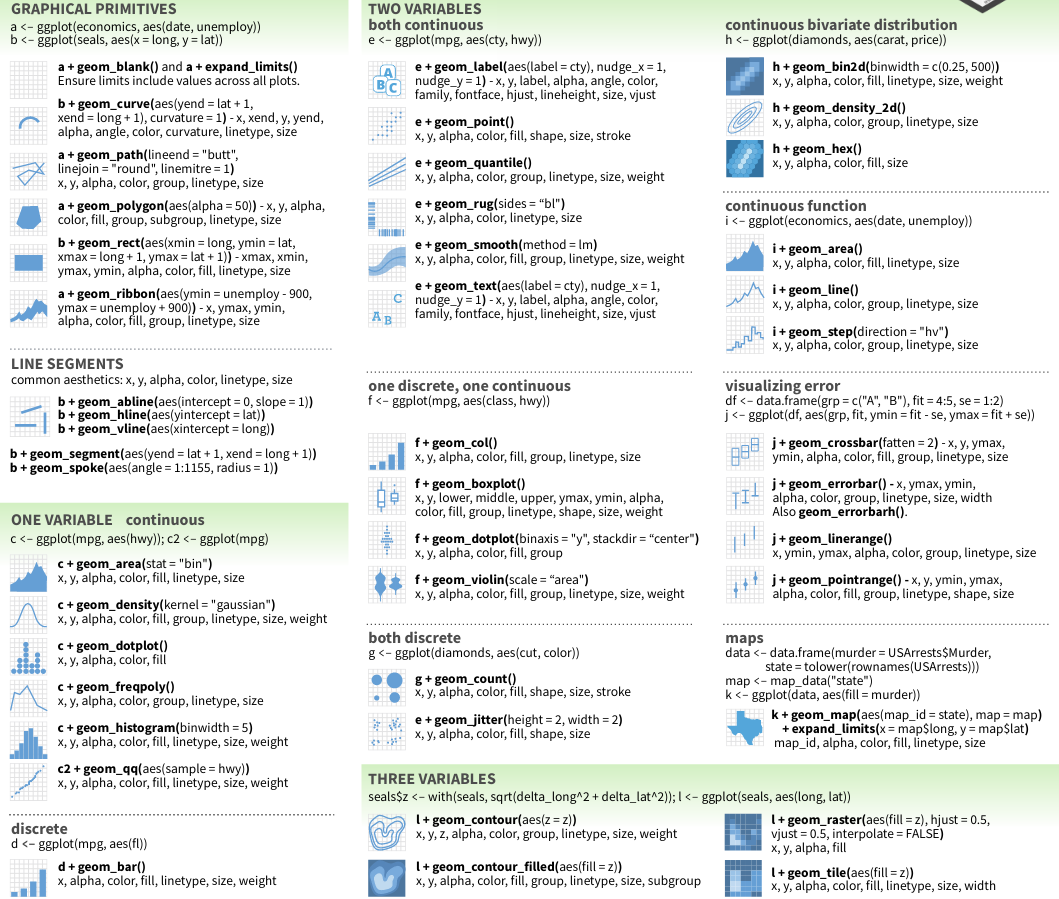
\includegraphics{assets/images/chapters/introduction-to-r/geom_cheatsheet.png}()\{width=55\%\}

\begin{itemize}
\tightlist
\item
  RStudio shares helpful cheatsheets for the tidyverse and beyond:
  \url{https://www.rstudio.com/resources/cheatsheets}
\end{itemize}

\hypertarget{scales-control-the-behaviour-of-visual-elements}{%
\subsection{\texorpdfstring{\texttt{scale}s control the behaviour of
visual
elements}{scales control the behaviour of visual elements}}\label{scales-control-the-behaviour-of-visual-elements}}

\begin{itemize}
\item
  Another plot: Boxplots of sample age through time

\begin{Shaded}
\begin{Highlighting}[]
\FunctionTok{ggplot}\NormalTok{(samples) }\SpecialCharTok{+}
\FunctionTok{geom\_boxplot}\NormalTok{(}\FunctionTok{aes}\NormalTok{(}\AttributeTok{x =} \FunctionTok{as.factor}\NormalTok{(publication\_year), }\AttributeTok{y =}\NormalTok{ sample\_age))}
\end{Highlighting}
\end{Shaded}
\item
  This is not well readable, because extreme outliers dictate the scale
\end{itemize}

\hypertarget{scales-control-the-behaviour-of-visual-elements-1}{%
\subsection{\texorpdfstring{\texttt{scale}s control the behaviour of
visual
elements}{scales control the behaviour of visual elements}}\label{scales-control-the-behaviour-of-visual-elements-1}}

\begin{itemize}
\item
  We can change the \textbf{scale} of different visual elements -
  e.g.~the y-axis

\begin{Shaded}
\begin{Highlighting}[]
\FunctionTok{ggplot}\NormalTok{(samples) }\SpecialCharTok{+}
\FunctionTok{geom\_boxplot}\NormalTok{(}\FunctionTok{aes}\NormalTok{(}\AttributeTok{x =} \FunctionTok{as.factor}\NormalTok{(publication\_year), }\AttributeTok{y =}\NormalTok{ sample\_age)) }\SpecialCharTok{+}
\FunctionTok{scale\_y\_log10}\NormalTok{()}
\end{Highlighting}
\end{Shaded}
\item
  The log-scale improves readability
\end{itemize}

\hypertarget{scales-control-the-behaviour-of-visual-elements-2}{%
\subsection{\texorpdfstring{\texttt{scale}s control the behaviour of
visual
elements}{scales control the behaviour of visual elements}}\label{scales-control-the-behaviour-of-visual-elements-2}}

\begin{itemize}
\item
  (Fill) color is a visual element of the plot and its scaling can be
  adjusted

\begin{Shaded}
\begin{Highlighting}[]
\FunctionTok{ggplot}\NormalTok{(samples) }\SpecialCharTok{+}
\FunctionTok{geom\_boxplot}\NormalTok{(}\FunctionTok{aes}\NormalTok{(}\AttributeTok{x =} \FunctionTok{as.factor}\NormalTok{(publication\_year), }\AttributeTok{y =}\NormalTok{ sample\_age,}
                \AttributeTok{fill =} \FunctionTok{as.factor}\NormalTok{(publication\_year))) }\SpecialCharTok{+}
\FunctionTok{scale\_y\_log10}\NormalTok{() }\SpecialCharTok{+} \FunctionTok{scale\_fill\_viridis\_d}\NormalTok{(}\AttributeTok{option =} \StringTok{"C"}\NormalTok{)}
\end{Highlighting}
\end{Shaded}
\end{itemize}

\hypertarget{defining-plot-matrices-via-facets}{%
\subsection{\texorpdfstring{Defining plot matrices via
\texttt{facet}s}{Defining plot matrices via facets}}\label{defining-plot-matrices-via-facets}}

\begin{itemize}
\item
  Splitting up the plot by categories into \textbf{facets} is another
  way to visualize more variables at once

\begin{Shaded}
\begin{Highlighting}[]
\FunctionTok{ggplot}\NormalTok{(samples) }\SpecialCharTok{+}
\FunctionTok{geom\_count}\NormalTok{(}\FunctionTok{aes}\NormalTok{(}\AttributeTok{x =} \FunctionTok{as.factor}\NormalTok{(publication\_year), }\AttributeTok{y =}\NormalTok{ material)) }\SpecialCharTok{+}
\FunctionTok{facet\_wrap}\NormalTok{(}\SpecialCharTok{\textasciitilde{}}\NormalTok{archive)}
\end{Highlighting}
\end{Shaded}
\item
  Unfortunately the x-axis became unreadable
\end{itemize}

\hypertarget{setting-purely-aesthetic-settings-with-theme}{%
\subsection{\texorpdfstring{Setting purely aesthetic settings with
\texttt{theme}}{Setting purely aesthetic settings with theme}}\label{setting-purely-aesthetic-settings-with-theme}}

\begin{itemize}
\item
  Aesthetic changes like this can be applied as part of the
  \texttt{theme}

\begin{Shaded}
\begin{Highlighting}[]
\FunctionTok{ggplot}\NormalTok{(samples) }\SpecialCharTok{+}
\FunctionTok{geom\_count}\NormalTok{(}\FunctionTok{aes}\NormalTok{(}\AttributeTok{x =} \FunctionTok{as.factor}\NormalTok{(publication\_year), }\AttributeTok{y =}\NormalTok{ material)) }\SpecialCharTok{+}
\FunctionTok{facet\_wrap}\NormalTok{(}\SpecialCharTok{\textasciitilde{}}\NormalTok{archive) }\SpecialCharTok{+}
\FunctionTok{theme}\NormalTok{(}\AttributeTok{axis.text.x =} \FunctionTok{element\_text}\NormalTok{(}\AttributeTok{angle =} \DecValTok{45}\NormalTok{, }\AttributeTok{hjust =} \DecValTok{1}\NormalTok{, }\AttributeTok{vjust =} \DecValTok{1}\NormalTok{))}
\end{Highlighting}
\end{Shaded}
\end{itemize}

\hypertarget{exercise-1}{%
\subsection{Exercise 1}\label{exercise-1}}

\begin{enumerate}
\def\labelenumi{\arabic{enumi}.}
\item
  Look at the \texttt{mtcars} dataset and read up on the meaning of its
  variables

\begin{Shaded}
\begin{Highlighting}[]

\end{Highlighting}
\end{Shaded}
\item
  Visualize the relationship between \emph{Gross horsepower} and
  \emph{1/4 mile time}

\begin{Shaded}
\begin{Highlighting}[]

\end{Highlighting}
\end{Shaded}
\item
  Integrate the \emph{Number of cylinders} into your plot

\begin{Shaded}
\begin{Highlighting}[]

\end{Highlighting}
\end{Shaded}
\end{enumerate}

\hypertarget{possible-solutions-1}{%
\subsection{Possible solutions 1}\label{possible-solutions-1}}

\begin{enumerate}
\def\labelenumi{\arabic{enumi}.}
\item
  Look at the \texttt{mtcars} dataset and read up on the meaning of its
  variables

\begin{Shaded}
\begin{Highlighting}[]
\NormalTok{?mtcars}
\end{Highlighting}
\end{Shaded}
\item
  Visualize the relationship between \emph{Gross horsepower} and
  \emph{1/4 mile time}

\begin{Shaded}
\begin{Highlighting}[]
\FunctionTok{ggplot}\NormalTok{(mtcars) }\SpecialCharTok{+} \FunctionTok{geom\_point}\NormalTok{(}\FunctionTok{aes}\NormalTok{(}\AttributeTok{x =}\NormalTok{ hp, }\AttributeTok{y =}\NormalTok{ qsec))}
\end{Highlighting}
\end{Shaded}
\item
  Integrate the \emph{Number of cylinders} into your plot

\begin{Shaded}
\begin{Highlighting}[]
\FunctionTok{ggplot}\NormalTok{(mtcars) }\SpecialCharTok{+} \FunctionTok{geom\_point}\NormalTok{(}\FunctionTok{aes}\NormalTok{(}\AttributeTok{x =}\NormalTok{ hp, }\AttributeTok{y =}\NormalTok{ qsec, }\AttributeTok{color =} \FunctionTok{as.factor}\NormalTok{(cyl)))}
\end{Highlighting}
\end{Shaded}
\end{enumerate}

\hypertarget{conditional-queries-on-tibbles}{%
\section{Conditional queries on
tibbles}\label{conditional-queries-on-tibbles}}

\hypertarget{selecting-columns-and-filtering-rows-with-select-and-filter}{%
\subsection{\texorpdfstring{Selecting columns and filtering rows with
\texttt{select} and
\texttt{filter}}{Selecting columns and filtering rows with select and filter}}\label{selecting-columns-and-filtering-rows-with-select-and-filter}}

\begin{itemize}
\item
  The \texttt{dplyr} package includes powerful functions to subset data
  in tibbles based on conditions
\item
  \texttt{dplyr::select} allows to select columns

\begin{Shaded}
\begin{Highlighting}[]
\NormalTok{dplyr}\SpecialCharTok{::}\FunctionTok{select}\NormalTok{(samples, project\_name, sample\_age)   }\CommentTok{\# reduce to two columns}
\NormalTok{dplyr}\SpecialCharTok{::}\FunctionTok{select}\NormalTok{(samples, }\SpecialCharTok{{-}}\NormalTok{project\_name, }\SpecialCharTok{{-}}\NormalTok{sample\_age) }\CommentTok{\# remove two columns}
\end{Highlighting}
\end{Shaded}
\item
  \texttt{dplyr::filter} allows for conditional filtering of rows

\begin{Shaded}
\begin{Highlighting}[]
\NormalTok{dplyr}\SpecialCharTok{::}\FunctionTok{filter}\NormalTok{(samples, publication\_year }\SpecialCharTok{==} \DecValTok{2014}\NormalTok{)  }\CommentTok{\# samples published in 2014}
\NormalTok{dplyr}\SpecialCharTok{::}\FunctionTok{filter}\NormalTok{(samples, publication\_year }\SpecialCharTok{==} \DecValTok{2014} \SpecialCharTok{|}
\NormalTok{                    publication\_year }\SpecialCharTok{==} \DecValTok{2018}\NormalTok{)  }\CommentTok{\# samples from 2015 OR 2018}
\NormalTok{dplyr}\SpecialCharTok{::}\FunctionTok{filter}\NormalTok{(samples, publication\_year }\SpecialCharTok{\%in\%} \FunctionTok{c}\NormalTok{(}\DecValTok{2014}\NormalTok{, }\DecValTok{2018}\NormalTok{)) }\CommentTok{\# match operator: \%in\%}
\NormalTok{dplyr}\SpecialCharTok{::}\FunctionTok{filter}\NormalTok{(samples, sample\_host }\SpecialCharTok{==} \StringTok{"Homo sapiens"} \SpecialCharTok{\&}
\NormalTok{                    community\_type }\SpecialCharTok{==} \StringTok{"oral"}\NormalTok{)  }\CommentTok{\# oral samples from modern humans}
\end{Highlighting}
\end{Shaded}
\end{itemize}

\hypertarget{chaining-functions-together-with-the-pipe}{%
\subsection{\texorpdfstring{Chaining functions together with the pipe
\texttt{\%\textgreater{}\%}}{Chaining functions together with the pipe \%\textgreater\%}}\label{chaining-functions-together-with-the-pipe}}

\begin{itemize}
\item
  The pipe \texttt{\%\textgreater{}\%} in the \texttt{magrittr} package
  is a clever infix operator to chain data and operations

\begin{Shaded}
\begin{Highlighting}[]
\FunctionTok{library}\NormalTok{(magrittr)}
\NormalTok{samples }\SpecialCharTok{\%\textgreater{}\%}\NormalTok{ dplyr}\SpecialCharTok{::}\FunctionTok{filter}\NormalTok{(publication\_year }\SpecialCharTok{==} \DecValTok{2014}\NormalTok{)}
\end{Highlighting}
\end{Shaded}
\item
  It forwards the LHS as the first argument of the function appearing on
  the RHS
\item
  That allows for sequences of functions (``tidyverse style'')

\begin{Shaded}
\begin{Highlighting}[]
\NormalTok{samples }\SpecialCharTok{\%\textgreater{}\%}
\NormalTok{dplyr}\SpecialCharTok{::}\FunctionTok{select}\NormalTok{(sample\_host, community\_type) }\SpecialCharTok{\%\textgreater{}\%}
\NormalTok{dplyr}\SpecialCharTok{::}\FunctionTok{filter}\NormalTok{(sample\_host }\SpecialCharTok{==} \StringTok{"Homo sapiens"} \SpecialCharTok{\&}\NormalTok{ community\_type }\SpecialCharTok{==} \StringTok{"oral"}\NormalTok{) }\SpecialCharTok{\%\textgreater{}\%}
\FunctionTok{nrow}\NormalTok{() }\CommentTok{\# count the rows}
\end{Highlighting}
\end{Shaded}
\item
  \texttt{magrittr} also offers some more operators, among which the
  extraction \texttt{\%\$\%} is particularly useful

\begin{Shaded}
\begin{Highlighting}[]
\NormalTok{samples }\SpecialCharTok{\%\textgreater{}\%}
\NormalTok{dplyr}\SpecialCharTok{::}\FunctionTok{filter}\NormalTok{(material }\SpecialCharTok{==} \StringTok{"tooth"}\NormalTok{) }\SpecialCharTok{\%$\%}
\NormalTok{sample\_age }\SpecialCharTok{\%\textgreater{}\%} \CommentTok{\# extract the sample\_age column as a vector}
\FunctionTok{max}\NormalTok{()          }\CommentTok{\# get the maximum of said vector}
\end{Highlighting}
\end{Shaded}
\end{itemize}

\hypertarget{summary-statistics-in-base-r}{%
\subsection{\texorpdfstring{Summary statistics in \texttt{base}
R}{Summary statistics in base R}}\label{summary-statistics-in-base-r}}

\begin{itemize}
\item
  Summarising and counting data is indispensable and R offers all
  operations you would expect in its \texttt{base} package

\begin{Shaded}
\begin{Highlighting}[]
\FunctionTok{nrow}\NormalTok{(samples)              }\CommentTok{\# number of rows in a tibble}
\FunctionTok{length}\NormalTok{(samples}\SpecialCharTok{$}\NormalTok{site\_name)  }\CommentTok{\# length/size of a vector}
\FunctionTok{unique}\NormalTok{(samples}\SpecialCharTok{$}\NormalTok{material)   }\CommentTok{\# unique elements of a vector}
\FunctionTok{min}\NormalTok{(samples}\SpecialCharTok{$}\NormalTok{sample\_age)    }\CommentTok{\# minimum}
\FunctionTok{max}\NormalTok{(samples}\SpecialCharTok{$}\NormalTok{sample\_age)    }\CommentTok{\# maximum}
\FunctionTok{mean}\NormalTok{(samples}\SpecialCharTok{$}\NormalTok{sample\_age)   }\CommentTok{\# mean}
\FunctionTok{median}\NormalTok{(samples}\SpecialCharTok{$}\NormalTok{sample\_age) }\CommentTok{\# median}
\FunctionTok{var}\NormalTok{(samples}\SpecialCharTok{$}\NormalTok{sample\_age)    }\CommentTok{\# variance}
\FunctionTok{sd}\NormalTok{(samples}\SpecialCharTok{$}\NormalTok{sample\_age)     }\CommentTok{\# standard deviation}
\FunctionTok{quantile}\NormalTok{(samples}\SpecialCharTok{$}\NormalTok{sample\_age, }\AttributeTok{probs =} \FloatTok{0.75}\NormalTok{) }\CommentTok{\# sample quantiles for the given probs}
\end{Highlighting}
\end{Shaded}
\item
  many of these functions can ignore missing values with an option
  \texttt{na.rm\ =\ TRUE}
\end{itemize}

\hypertarget{group-wise-summaries-with-group_by-and-summarise}{%
\subsection{\texorpdfstring{Group-wise summaries with \texttt{group\_by}
and
\texttt{summarise}}{Group-wise summaries with group\_by and summarise}}\label{group-wise-summaries-with-group_by-and-summarise}}

\begin{itemize}
\item
  These summary statistics are particular useful when applied to
  conditional subsets of a dataset
\item
  \texttt{dplyr} allows such summary operations with a combination of
  \texttt{group\_by} and \texttt{summarise}

\begin{Shaded}
\begin{Highlighting}[]
\NormalTok{samples }\SpecialCharTok{\%\textgreater{}\%}
\NormalTok{dplyr}\SpecialCharTok{::}\FunctionTok{group\_by}\NormalTok{(material) }\SpecialCharTok{\%\textgreater{}\%}  \CommentTok{\# group the tibble by the material column}
\NormalTok{dplyr}\SpecialCharTok{::}\FunctionTok{summarise}\NormalTok{(}
    \AttributeTok{min\_age =} \FunctionTok{min}\NormalTok{(sample\_age),   }\CommentTok{\# a new column: min age for each group}
    \AttributeTok{median\_age =} \FunctionTok{median}\NormalTok{(sample\_age), }\CommentTok{\# a new column: median age for each group}
    \AttributeTok{max\_age =} \FunctionTok{max}\NormalTok{(sample\_age)    }\CommentTok{\# a new column: max age for each group}
\NormalTok{)}
\end{Highlighting}
\end{Shaded}
\item
  grouping can be applied across multiple columns

\begin{Shaded}
\begin{Highlighting}[]
\NormalTok{samples }\SpecialCharTok{\%\textgreater{}\%}
\NormalTok{dplyr}\SpecialCharTok{::}\FunctionTok{group\_by}\NormalTok{(material, sample\_host) }\SpecialCharTok{\%\textgreater{}\%} \CommentTok{\# group by material and host}
\NormalTok{dplyr}\SpecialCharTok{::}\FunctionTok{summarise}\NormalTok{(}
    \AttributeTok{n =}\NormalTok{ dplyr}\SpecialCharTok{::}\FunctionTok{n}\NormalTok{(),  }\CommentTok{\# a new column: number of samples for each group}
    \AttributeTok{.groups =} \StringTok{"drop"} \CommentTok{\# drop the grouping after this summary operation}
\NormalTok{)}
\end{Highlighting}
\end{Shaded}
\end{itemize}

\hypertarget{sorting-and-slicing-tibbles-with-arrange-and-slice}{%
\subsection{\texorpdfstring{Sorting and slicing tibbles with
\texttt{arrange} and
\texttt{slice}}{Sorting and slicing tibbles with arrange and slice}}\label{sorting-and-slicing-tibbles-with-arrange-and-slice}}

\begin{itemize}
\item
  \texttt{dplyr} allows to \texttt{arrange} tibbles by one or multiple
  columns

\begin{Shaded}
\begin{Highlighting}[]
\NormalTok{samples }\SpecialCharTok{\%\textgreater{}\%}\NormalTok{ dplyr}\SpecialCharTok{::}\FunctionTok{arrange}\NormalTok{(publication\_year)        }\CommentTok{\# sort by publication year}
\NormalTok{samples }\SpecialCharTok{\%\textgreater{}\%}\NormalTok{ dplyr}\SpecialCharTok{::}\FunctionTok{arrange}\NormalTok{(publication\_year,}
\NormalTok{                        sample\_age)              }\CommentTok{\# ... and sample age}
\NormalTok{samples }\SpecialCharTok{\%\textgreater{}\%}\NormalTok{ dplyr}\SpecialCharTok{::}\FunctionTok{arrange}\NormalTok{(dplyr}\SpecialCharTok{::}\FunctionTok{desc}\NormalTok{(sample\_age)) }\CommentTok{\# sort descending on sample age}
\end{Highlighting}
\end{Shaded}
\item
  Sorting also works within groups and can be paired with \texttt{slice}
  to extract extreme values per group

\begin{Shaded}
\begin{Highlighting}[]
\NormalTok{samples }\SpecialCharTok{\%\textgreater{}\%}
\NormalTok{dplyr}\SpecialCharTok{::}\FunctionTok{group\_by}\NormalTok{(publication\_year) }\SpecialCharTok{\%\textgreater{}\%}       \CommentTok{\# group by publication year}
\NormalTok{dplyr}\SpecialCharTok{::}\FunctionTok{arrange}\NormalTok{(dplyr}\SpecialCharTok{::}\FunctionTok{desc}\NormalTok{(sample\_age)) }\SpecialCharTok{\%\textgreater{}\%} \CommentTok{\# sort by age within (!) groups}
\NormalTok{dplyr}\SpecialCharTok{::}\FunctionTok{slice\_head}\NormalTok{(}\AttributeTok{n =} \DecValTok{2}\NormalTok{) }\SpecialCharTok{\%\textgreater{}\%}                \CommentTok{\# keep the first two samples per group}
\NormalTok{dplyr}\SpecialCharTok{::}\FunctionTok{ungroup}\NormalTok{()                            }\CommentTok{\# remove the still lingering grouping}
\end{Highlighting}
\end{Shaded}
\item
  Slicing is also the relevant operation to take random samples from the
  observations in a tibble

\begin{Shaded}
\begin{Highlighting}[]
\NormalTok{samples }\SpecialCharTok{\%\textgreater{}\%}\NormalTok{ dplyr}\SpecialCharTok{::}\FunctionTok{slice\_sample}\NormalTok{(}\AttributeTok{n =} \DecValTok{20}\NormalTok{)}
\end{Highlighting}
\end{Shaded}
\end{itemize}

\hypertarget{exercise-2}{%
\subsection{Exercise 2}\label{exercise-2}}

\begin{enumerate}
\def\labelenumi{\arabic{enumi}.}
\item
  Determine the number of cars with four \emph{forward gears}
  (\texttt{gear}) in the \texttt{mtcars} dataset

\begin{Shaded}
\begin{Highlighting}[]

\end{Highlighting}
\end{Shaded}
\item
  Determine the mean \emph{1/4 mile time} (\texttt{qsec}) per
  \emph{Number of cylinders} (\texttt{cyl}) group

\begin{Shaded}
\begin{Highlighting}[]

\end{Highlighting}
\end{Shaded}
\item
  Identify the least efficient cars for both \emph{transmission types}
  (\texttt{am})

\begin{Shaded}
\begin{Highlighting}[]

\end{Highlighting}
\end{Shaded}
\end{enumerate}

\hypertarget{possible-solutions-2}{%
\subsection{Possible solutions 2}\label{possible-solutions-2}}

\begin{enumerate}
\def\labelenumi{\arabic{enumi}.}
\item
  Determine the number of cars with four \emph{forward gears}
  (\texttt{gear}) in the \texttt{mtcars} dataset

\begin{Shaded}
\begin{Highlighting}[]
\NormalTok{mtcars }\SpecialCharTok{\%\textgreater{}\%}\NormalTok{ dplyr}\SpecialCharTok{::}\FunctionTok{filter}\NormalTok{(gear }\SpecialCharTok{==} \DecValTok{4}\NormalTok{) }\SpecialCharTok{\%\textgreater{}\%} \FunctionTok{nrow}\NormalTok{()}
\end{Highlighting}
\end{Shaded}
\item
  Determine the mean \emph{1/4 mile time} (\texttt{qsec}) per
  \emph{Number of cylinders} (\texttt{cyl}) group

\begin{Shaded}
\begin{Highlighting}[]
\NormalTok{mtcars }\SpecialCharTok{\%\textgreater{}\%}\NormalTok{ dplyr}\SpecialCharTok{::}\FunctionTok{group\_by}\NormalTok{(cyl) }\SpecialCharTok{\%\textgreater{}\%}\NormalTok{ dplyr}\SpecialCharTok{::}\FunctionTok{summarise}\NormalTok{(}\AttributeTok{qsec\_mean =} \FunctionTok{mean}\NormalTok{(qsec))}
\end{Highlighting}
\end{Shaded}
\item
  Identify the least efficient cars for both \emph{transmission types}
  (\texttt{am})

\begin{Shaded}
\begin{Highlighting}[]
\CommentTok{\#mtcars3 \textless{}{-} tibble::rownames\_to\_column(mtcars, var = "car") \%\textgreater{}\% tibble::as\_tibble()}
\NormalTok{mtcars }\SpecialCharTok{\%\textgreater{}\%}\NormalTok{ dplyr}\SpecialCharTok{::}\FunctionTok{group\_by}\NormalTok{(am) }\SpecialCharTok{\%\textgreater{}\%}\NormalTok{ dplyr}\SpecialCharTok{::}\FunctionTok{arrange}\NormalTok{(mpg) }\SpecialCharTok{\%\textgreater{}\%}\NormalTok{ dplyr}\SpecialCharTok{::}\FunctionTok{slice\_head}\NormalTok{()}
\end{Highlighting}
\end{Shaded}
\end{enumerate}

\hypertarget{transforming-and-manipulating-tibbles}{%
\section{Transforming and manipulating
tibbles}\label{transforming-and-manipulating-tibbles}}

\hypertarget{renaming-and-reordering-columns-and-values-with-rename-relocate-and-recode}{%
\subsection{\texorpdfstring{Renaming and reordering columns and values
with \texttt{rename}, \texttt{relocate} and
\texttt{recode}}{Renaming and reordering columns and values with rename, relocate and recode}}\label{renaming-and-reordering-columns-and-values-with-rename-relocate-and-recode}}

\begin{itemize}
\item
  Columns in tibbles can be renamed with \texttt{dplyr::rename} and
  reordered with \texttt{dplyr::relocate}

\begin{Shaded}
\begin{Highlighting}[]
\NormalTok{samples }\SpecialCharTok{\%\textgreater{}\%}\NormalTok{ dplyr}\SpecialCharTok{::}\FunctionTok{rename}\NormalTok{(}\AttributeTok{country =}\NormalTok{ geo\_loc\_name) }\CommentTok{\# rename a column}
\NormalTok{samples }\SpecialCharTok{\%\textgreater{}\%}\NormalTok{ dplyr}\SpecialCharTok{::}\FunctionTok{relocate}\NormalTok{(site\_name, }\AttributeTok{.before =}\NormalTok{ project\_name) }\CommentTok{\# reorder columns}
\end{Highlighting}
\end{Shaded}
\item
  Values in columns can also be changed with \texttt{dplyr::recode}

\begin{Shaded}
\begin{Highlighting}[]
\NormalTok{samples}\SpecialCharTok{$}\NormalTok{sample\_host }\SpecialCharTok{\%\textgreater{}\%}\NormalTok{ dplyr}\SpecialCharTok{::}\FunctionTok{recode}\NormalTok{(}\StringTok{\textasciigrave{}}\AttributeTok{Homo sapiens}\StringTok{\textasciigrave{}} \OtherTok{=} \StringTok{"modern human"}\NormalTok{)}
\end{Highlighting}
\end{Shaded}
\item
  R supports explicitly ordinal data with \texttt{factor}s, which can be
  reordered as well
\item
  \texttt{factor}s can be handeld more easily with the \texttt{forcats}
  package

\begin{Shaded}
\begin{Highlighting}[]
\FunctionTok{ggplot}\NormalTok{(samples) }\SpecialCharTok{+} \FunctionTok{geom\_bar}\NormalTok{(}\FunctionTok{aes}\NormalTok{(}\AttributeTok{x =}\NormalTok{ community\_type)) }\CommentTok{\# bars are alphabetically ordered}
\NormalTok{sa2 }\OtherTok{\textless{}{-}}\NormalTok{ samples}
\NormalTok{sa2}\SpecialCharTok{$}\NormalTok{cto }\OtherTok{\textless{}{-}}\NormalTok{ forcats}\SpecialCharTok{::}\FunctionTok{fct\_reorder}\NormalTok{(sa2}\SpecialCharTok{$}\NormalTok{community\_type, sa2}\SpecialCharTok{$}\NormalTok{community\_type, length)}
\CommentTok{\# fct\_reorder: reorder the input factor by a summary statistic on an other vector}
\FunctionTok{ggplot}\NormalTok{(sa2) }\SpecialCharTok{+} \FunctionTok{geom\_bar}\NormalTok{(}\FunctionTok{aes}\NormalTok{(}\AttributeTok{x =}\NormalTok{ community\_type)) }\CommentTok{\# bars are ordered by size}
\end{Highlighting}
\end{Shaded}
\end{itemize}

\hypertarget{adding-columns-to-tibbles-with-mutate-and-transmute}{%
\subsection{\texorpdfstring{Adding columns to tibbles with
\texttt{mutate} and
\texttt{transmute}}{Adding columns to tibbles with mutate and transmute}}\label{adding-columns-to-tibbles-with-mutate-and-transmute}}

\begin{itemize}
\item
  A common application of data manipulation is adding derived columns.
  \texttt{dplyr} offers that with \texttt{mutate}

\begin{Shaded}
\begin{Highlighting}[]
\NormalTok{samples }\SpecialCharTok{\%\textgreater{}\%}
\NormalTok{dplyr}\SpecialCharTok{::}\FunctionTok{mutate}\NormalTok{(                                               }\CommentTok{\# add a column that}
    \AttributeTok{archive\_summary =} \FunctionTok{paste0}\NormalTok{(archive, }\StringTok{": "}\NormalTok{, archive\_accession) }\CommentTok{\# combines two other}
\NormalTok{) }\SpecialCharTok{\%$\%}\NormalTok{ archive\_summary                                        }\CommentTok{\# columns}
\end{Highlighting}
\end{Shaded}
\item
  \texttt{dplyr::transmute} removes all columns but the newly created
  ones

\begin{Shaded}
\begin{Highlighting}[]
\NormalTok{samples }\SpecialCharTok{\%\textgreater{}\%}
\NormalTok{dplyr}\SpecialCharTok{::}\FunctionTok{transmute}\NormalTok{(}
    \AttributeTok{sample\_name =} \FunctionTok{tolower}\NormalTok{(sample\_name), }\CommentTok{\# overwrite this columns}
\NormalTok{    publication\_doi                     }\CommentTok{\# select this column}
\NormalTok{)}
\end{Highlighting}
\end{Shaded}
\item
  \texttt{tibble::add\_column} behaves as \texttt{dplyr::mutate}, but
  gives more control over column position

\begin{Shaded}
\begin{Highlighting}[]
\NormalTok{samples }\SpecialCharTok{\%\textgreater{}\%}\NormalTok{ tibble}\SpecialCharTok{::}\FunctionTok{add\_column}\NormalTok{(., }\AttributeTok{id =} \DecValTok{1}\SpecialCharTok{:}\FunctionTok{nrow}\NormalTok{(.), }\AttributeTok{.before =} \StringTok{"project\_name"}\NormalTok{)}
\end{Highlighting}
\end{Shaded}
\end{itemize}

\hypertarget{conditional-operations-with-ifelse-and-case_when}{%
\subsection{\texorpdfstring{Conditional operations with \texttt{ifelse}
and
\texttt{case\_when}}{Conditional operations with ifelse and case\_when}}\label{conditional-operations-with-ifelse-and-case_when}}

\begin{itemize}
\item
  \texttt{ifelse} allows to implement conditional \texttt{mutate}
  operations, that consider information from other columns, but that
  gets cumbersome easily

\begin{Shaded}
\begin{Highlighting}[]
\NormalTok{samples }\SpecialCharTok{\%\textgreater{}\%}\NormalTok{ dplyr}\SpecialCharTok{::}\FunctionTok{mutate}\NormalTok{(}\AttributeTok{hemi =} \FunctionTok{ifelse}\NormalTok{(latitude }\SpecialCharTok{\textgreater{}=} \DecValTok{0}\NormalTok{, }\StringTok{"North"}\NormalTok{, }\StringTok{"South"}\NormalTok{)) }\SpecialCharTok{\%$\%}\NormalTok{ hemi}

\NormalTok{samples }\SpecialCharTok{\%\textgreater{}\%}\NormalTok{ dplyr}\SpecialCharTok{::}\FunctionTok{mutate}\NormalTok{(}
\AttributeTok{hemi =} \FunctionTok{ifelse}\NormalTok{(}\FunctionTok{is.na}\NormalTok{(latitude), }\StringTok{"unknown"}\NormalTok{, }\FunctionTok{ifelse}\NormalTok{(latitude }\SpecialCharTok{\textgreater{}=} \DecValTok{0}\NormalTok{, }\StringTok{"North"}\NormalTok{, }\StringTok{"South"}\NormalTok{))}
\NormalTok{) }\SpecialCharTok{\%$\%}\NormalTok{ hemi}
\end{Highlighting}
\end{Shaded}
\item
  \texttt{dplyr::case\_when} is a much more readable solution for this
  application

\begin{Shaded}
\begin{Highlighting}[]
\NormalTok{samples }\SpecialCharTok{\%\textgreater{}\%}\NormalTok{ dplyr}\SpecialCharTok{::}\FunctionTok{mutate}\NormalTok{(}
\AttributeTok{hemi =}\NormalTok{ dplyr}\SpecialCharTok{::}\FunctionTok{case\_when}\NormalTok{(}
\NormalTok{    latitude }\SpecialCharTok{\textgreater{}=} \DecValTok{0} \SpecialCharTok{\textasciitilde{}} \StringTok{"North"}\NormalTok{,}
\NormalTok{    latitude }\SpecialCharTok{\textless{}} \DecValTok{0}  \SpecialCharTok{\textasciitilde{}} \StringTok{"South"}\NormalTok{,}
    \ConstantTok{TRUE}          \SpecialCharTok{\textasciitilde{}} \StringTok{"unknown"} \CommentTok{\# TRUE catches all remaining cases}
\NormalTok{)}
\NormalTok{) }\SpecialCharTok{\%$\%}\NormalTok{ hemi}
\end{Highlighting}
\end{Shaded}
\end{itemize}

\hypertarget{long-and-wide-data-formats}{%
\subsection{Long and wide data
formats}\label{long-and-wide-data-formats}}

\begin{itemize}
\tightlist
\item
  For different applications or to simplify certain analysis or plotting
  operations data often has to be transformed from a \textbf{wide} to a
  \textbf{long} format or vice versa
\end{itemize}

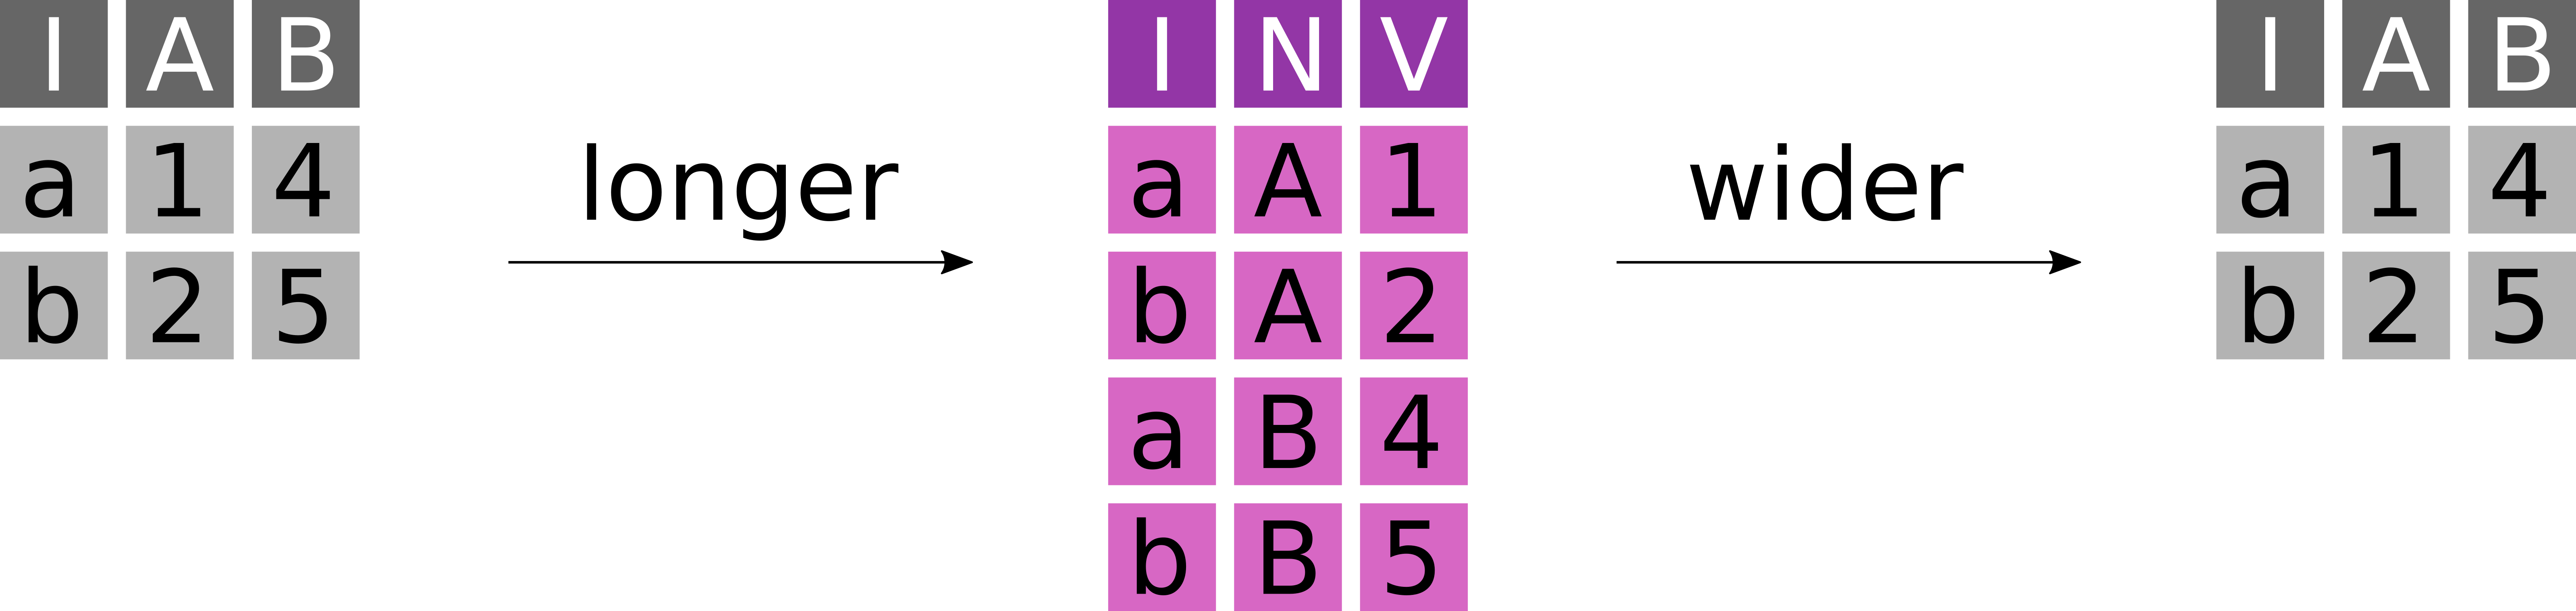
\includegraphics{assets/images/chapters/introduction-to-r/pivot_longer_wider.png}

\begin{itemize}
\tightlist
\item
  A table in \textbf{wide} format has N key columns and N value columns
\item
  A table in \textbf{long} format has N key columns, one descriptor
  column and one value column
\end{itemize}

\hypertarget{a-wide-dataset}{%
\subsection{A wide dataset}\label{a-wide-dataset}}

\begin{Shaded}
\begin{Highlighting}[]
\NormalTok{carsales }\OtherTok{\textless{}{-}}\NormalTok{ tibble}\SpecialCharTok{::}\FunctionTok{tribble}\NormalTok{(}
  \SpecialCharTok{\textasciitilde{}}\NormalTok{brand, }\SpecialCharTok{\textasciitilde{}}\StringTok{\textasciigrave{}}\AttributeTok{2014}\StringTok{\textasciigrave{}}\NormalTok{, }\SpecialCharTok{\textasciitilde{}}\StringTok{\textasciigrave{}}\AttributeTok{2015}\StringTok{\textasciigrave{}}\NormalTok{, }\SpecialCharTok{\textasciitilde{}}\StringTok{\textasciigrave{}}\AttributeTok{2016}\StringTok{\textasciigrave{}}\NormalTok{, }\SpecialCharTok{\textasciitilde{}}\StringTok{\textasciigrave{}}\AttributeTok{2017}\StringTok{\textasciigrave{}}\NormalTok{,}
  \StringTok{"BMW"}\NormalTok{,  }\DecValTok{20}\NormalTok{,      }\DecValTok{25}\NormalTok{,      }\DecValTok{30}\NormalTok{,      }\DecValTok{45}\NormalTok{,}
  \StringTok{"VW"}\NormalTok{,   }\DecValTok{67}\NormalTok{,      }\DecValTok{40}\NormalTok{,     }\DecValTok{120}\NormalTok{,      }\DecValTok{55}
\NormalTok{)}

\NormalTok{carsales}
\end{Highlighting}
\end{Shaded}

\begin{itemize}
\tightlist
\item
  Wide format becomes a problem, when the columns are semantically
  identical. This dataset is in wide format and we can not easily plot
  it
\item
  We generally prefer data in long format, although it is more verbose
  with more duplication. ``Long'' format data is more ``tidy''
\end{itemize}

\hypertarget{making-a-wide-dataset-long-with-pivot_longer}{%
\subsection{\texorpdfstring{Making a wide dataset long with
\texttt{pivot\_longer}}{Making a wide dataset long with pivot\_longer}}\label{making-a-wide-dataset-long-with-pivot_longer}}

\begin{Shaded}
\begin{Highlighting}[]
\NormalTok{carsales\_long }\OtherTok{\textless{}{-}}\NormalTok{ carsales }\SpecialCharTok{\%\textgreater{}\%}\NormalTok{ tidyr}\SpecialCharTok{::}\FunctionTok{pivot\_longer}\NormalTok{(}
  \AttributeTok{cols =}\NormalTok{ tidyselect}\SpecialCharTok{::}\FunctionTok{num\_range}\NormalTok{(}\StringTok{""}\NormalTok{, }\AttributeTok{range =} \DecValTok{2014}\SpecialCharTok{:}\DecValTok{2017}\NormalTok{), }\CommentTok{\# set of columns to transform}
  \AttributeTok{names\_to =} \StringTok{"year"}\NormalTok{,            }\CommentTok{\# the name of the descriptor column we want}
  \AttributeTok{names\_transform =}\NormalTok{ as.integer, }\CommentTok{\# a transformation function to apply to the names}
  \AttributeTok{values\_to =} \StringTok{"sales"}           \CommentTok{\# the name of the value column we want}
\NormalTok{)}

\NormalTok{carsales\_long}
\end{Highlighting}
\end{Shaded}

\hypertarget{making-a-long-dataset-wide-with-pivot_wider}{%
\subsection{\texorpdfstring{Making a long dataset wide with
\texttt{pivot\_wider}}{Making a long dataset wide with pivot\_wider}}\label{making-a-long-dataset-wide-with-pivot_wider}}

\begin{Shaded}
\begin{Highlighting}[]
\NormalTok{carsales\_wide }\OtherTok{\textless{}{-}}\NormalTok{ carsales\_long }\SpecialCharTok{\%\textgreater{}\%}\NormalTok{ tidyr}\SpecialCharTok{::}\FunctionTok{pivot\_wider}\NormalTok{(}
  \AttributeTok{id\_cols =} \StringTok{"brand"}\NormalTok{,  }\CommentTok{\# the set of id columns that should not be changed}
  \AttributeTok{names\_from =}\NormalTok{ year,  }\CommentTok{\# the descriptor column with the names of the new columns}
  \AttributeTok{values\_from =}\NormalTok{ sales }\CommentTok{\# the value column from which the values should be extracted}
\NormalTok{)}

\NormalTok{carsales\_wide}
\end{Highlighting}
\end{Shaded}

\begin{itemize}
\tightlist
\item
  Applications of wide datasets are adjacency matrices to represent
  graphs, covariance matrices or other pairwise statistics
\item
  When data gets big, then wide formats can be significantly more
  efficient (e.g.~for spatial data)
\end{itemize}

\hypertarget{exercise-3}{%
\subsection{Exercise 3}\label{exercise-3}}

\begin{enumerate}
\def\labelenumi{\arabic{enumi}.}
\item
  Move the column \texttt{gear} to the first position of the mtcars
  dataset

\begin{Shaded}
\begin{Highlighting}[]

\end{Highlighting}
\end{Shaded}
\item
  Make a new dataset \texttt{mtcars2} with the column \texttt{mpg} and
  an additional column \texttt{am\_v}, which encodes the
  \emph{transmission type} (\texttt{am}) as either \texttt{"manual"} or
  \texttt{"automatic"}

\begin{Shaded}
\begin{Highlighting}[]

\end{Highlighting}
\end{Shaded}
\item
  Count the number of cars per \emph{transmission type} (\texttt{am\_v})
  and \emph{number of gears} (\texttt{gear}). Then transform the result
  to a wide format, with one column per \emph{transmission type}.

\begin{Shaded}
\begin{Highlighting}[]

\end{Highlighting}
\end{Shaded}
\end{enumerate}

\hypertarget{possible-solutions-3}{%
\subsection{Possible solutions 3}\label{possible-solutions-3}}

\begin{enumerate}
\def\labelenumi{\arabic{enumi}.}
\item
  Move the column \texttt{gear} to the first position of the mtcars
  dataset

\begin{Shaded}
\begin{Highlighting}[]
\NormalTok{mtcars }\SpecialCharTok{\%\textgreater{}\%}\NormalTok{ dplyr}\SpecialCharTok{::}\FunctionTok{relocate}\NormalTok{(gear, }\AttributeTok{.before =}\NormalTok{ mpg)}
\end{Highlighting}
\end{Shaded}
\item
  Make a new dataset \texttt{mtcars2} with the column \texttt{gear} and
  an additional column \texttt{am\_v}, which encodes the
  \emph{transmission type} (\texttt{am}) as either \texttt{"manual"} or
  \texttt{"automatic"}

\begin{Shaded}
\begin{Highlighting}[]
\NormalTok{mtcars2 }\OtherTok{\textless{}{-}}\NormalTok{ mtcars }\SpecialCharTok{\%\textgreater{}\%}\NormalTok{ dplyr}\SpecialCharTok{::}\FunctionTok{mutate}\NormalTok{(}
\NormalTok{gear, }\AttributeTok{am\_v =}\NormalTok{ dplyr}\SpecialCharTok{::}\FunctionTok{case\_when}\NormalTok{(am }\SpecialCharTok{==} \DecValTok{0} \SpecialCharTok{\textasciitilde{}} \StringTok{"automatic"}\NormalTok{, am }\SpecialCharTok{==} \DecValTok{1} \SpecialCharTok{\textasciitilde{}} \StringTok{"manual"}\NormalTok{)}
\NormalTok{)}
\end{Highlighting}
\end{Shaded}
\item
  Count the number of cars in \texttt{mtcars2} per \emph{transmission
  type} (\texttt{am\_v}) and \emph{number of gears} (\texttt{gear}).
  Then transform the result to a wide format, with one column per
  \emph{transmission type}.

\begin{Shaded}
\begin{Highlighting}[]
\NormalTok{mtcars2 }\SpecialCharTok{\%\textgreater{}\%}\NormalTok{ dplyr}\SpecialCharTok{::}\FunctionTok{group\_by}\NormalTok{(am\_v, gear) }\SpecialCharTok{\%\textgreater{}\%}\NormalTok{ dplyr}\SpecialCharTok{::}\FunctionTok{tally}\NormalTok{() }\SpecialCharTok{\%\textgreater{}\%}
\NormalTok{tidyr}\SpecialCharTok{::}\FunctionTok{pivot\_wider}\NormalTok{(}\AttributeTok{names\_from =}\NormalTok{ am\_v, }\AttributeTok{values\_from =}\NormalTok{ n)}
\end{Highlighting}
\end{Shaded}
\end{enumerate}

\hypertarget{combining-tibbles-with-join-operations}{%
\section{Combining tibbles with join
operations}\label{combining-tibbles-with-join-operations}}

\hypertarget{types-of-joins}{%
\subsection{Types of joins}\label{types-of-joins}}

Joins combine two datasets x and y based on key columns

\begin{itemize}
\tightlist
\item
  Mutating joins add columns from one dataset to the other

  \begin{itemize}
  \tightlist
  \item
    Left join: Take observations from x and add fitting information from
    y
  \item
    Right join: Take observations from y and add fitting information
    from x
  \item
    Inner join: Join the overlapping observations from x and y
  \item
    Full join: Join all observations from x and y, even if information
    is missing
  \end{itemize}
\item
  Filtering joins remove observations from x based on their presence in
  y

  \begin{itemize}
  \tightlist
  \item
    Semi join: Keep every observation in x that is in y
  \item
    Anti join: Keep every observation in x that is not in y
  \end{itemize}
\end{itemize}

\hypertarget{a-second-dataset}{%
\subsection{A second dataset}\label{a-second-dataset}}

\begin{Shaded}
\begin{Highlighting}[]
\NormalTok{library\_table\_path }\OtherTok{\textless{}{-}} \StringTok{"/vol/volume/3b{-}1{-}introduction{-}to{-}r{-}and{-}the{-}tidyverse/ancientmetagenome{-}hostassociated\_libraries.tsv"}
\NormalTok{library\_table\_url }\OtherTok{\textless{}{-}}
\StringTok{"https://raw.githubusercontent.com/SPAAM{-}community/AncientMetagenomeDir/b187df6ebd23dfeb42935fd5020cb615ead3f164/}
\StringTok{ancientmetagenome{-}hostassociated/libraries/ancientmetagenome{-}hostassociated\_libraries.tsv"}

\NormalTok{libraries }\OtherTok{\textless{}{-}}\NormalTok{ readr}\SpecialCharTok{::}\FunctionTok{read\_tsv}\NormalTok{(library\_table\_url)}
\FunctionTok{print}\NormalTok{(libraries, }\AttributeTok{n =} \DecValTok{3}\NormalTok{)}
\end{Highlighting}
\end{Shaded}

\hypertarget{meaningful-subsets}{%
\subsection{Meaningful subsets}\label{meaningful-subsets}}

\begin{Shaded}
\begin{Highlighting}[]
\NormalTok{samsub }\OtherTok{\textless{}{-}}\NormalTok{ samples }\SpecialCharTok{\%\textgreater{}\%}\NormalTok{ dplyr}\SpecialCharTok{::}\FunctionTok{select}\NormalTok{(project\_name, sample\_name, sample\_age)}
\NormalTok{libsub }\OtherTok{\textless{}{-}}\NormalTok{ libraries }\SpecialCharTok{\%\textgreater{}\%}\NormalTok{ dplyr}\SpecialCharTok{::}\FunctionTok{select}\NormalTok{(project\_name, sample\_name, library\_name, read\_count)}
\end{Highlighting}
\end{Shaded}

\begin{Shaded}
\begin{Highlighting}[]
\FunctionTok{print}\NormalTok{(samsub, }\AttributeTok{n =} \DecValTok{3}\NormalTok{)}
\FunctionTok{print}\NormalTok{(libsub, }\AttributeTok{n =} \DecValTok{3}\NormalTok{)}
\end{Highlighting}
\end{Shaded}

\hypertarget{left-join}{%
\subsection{Left join}\label{left-join}}

Take observations from x and add fitting information from y

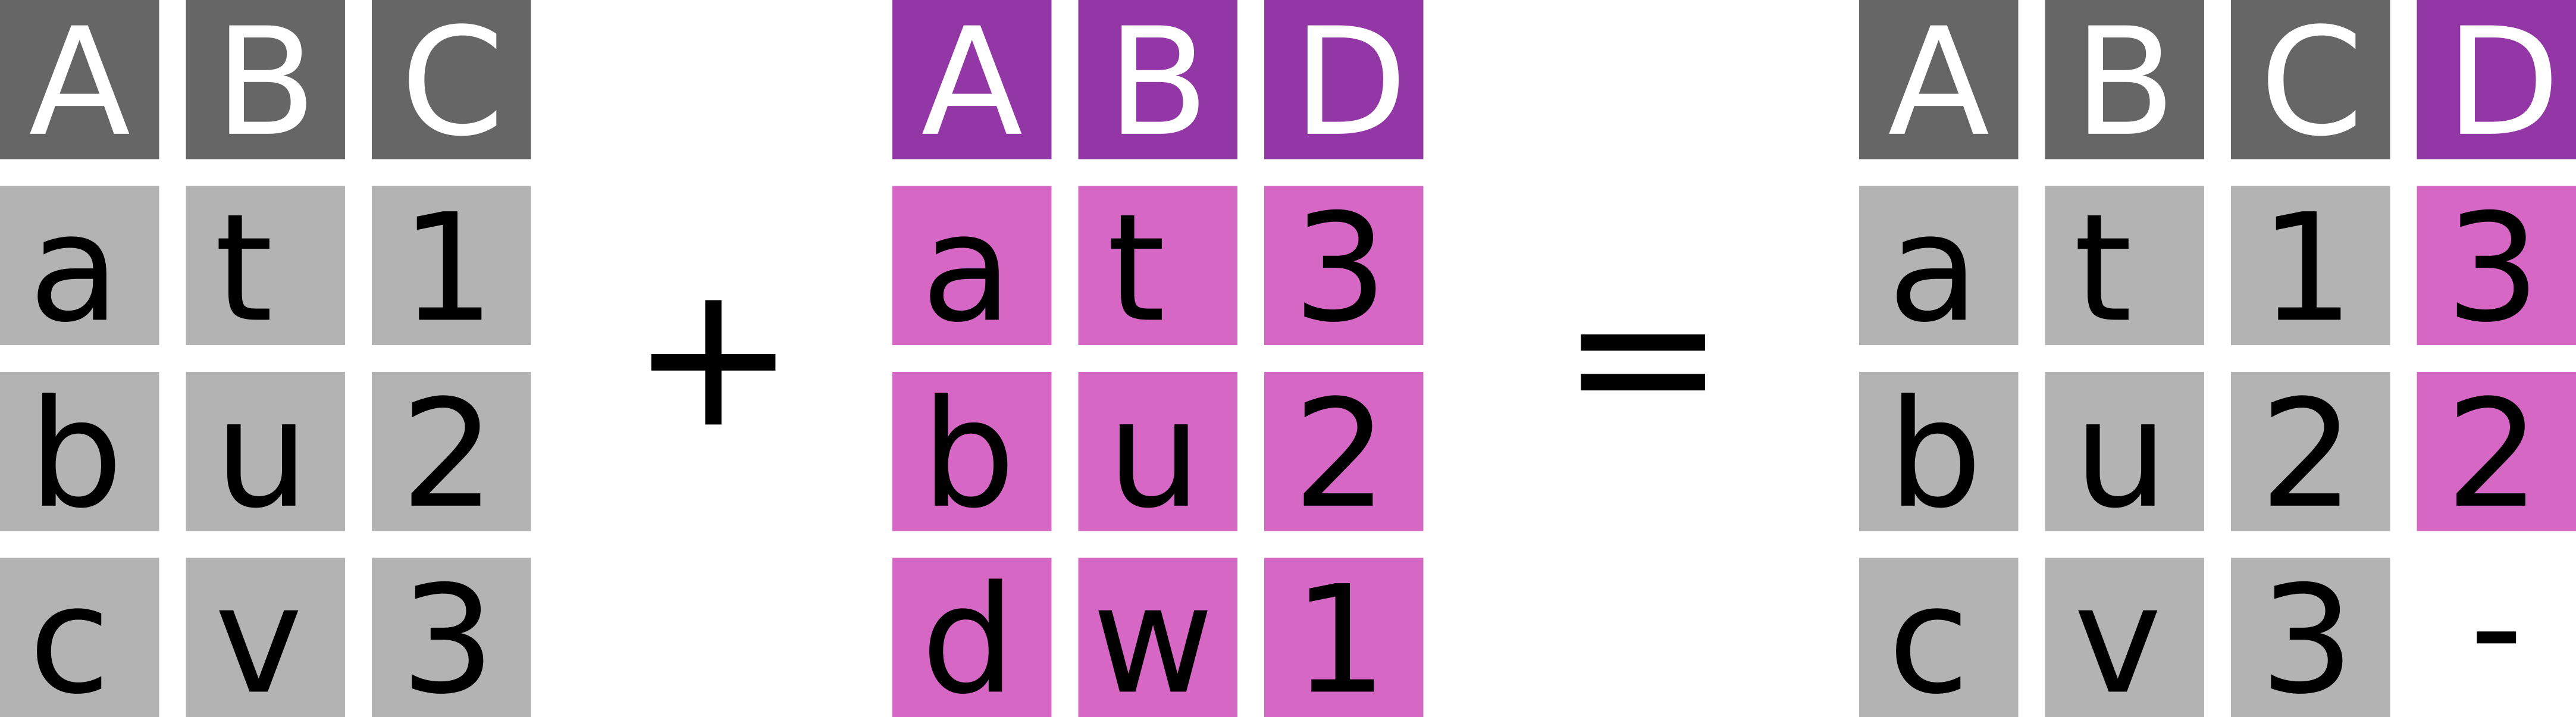
\includegraphics{assets/images/chapters/introduction-to-r/left_join.png}

\begin{Shaded}
\begin{Highlighting}[]
\NormalTok{left }\OtherTok{\textless{}{-}}\NormalTok{ dplyr}\SpecialCharTok{::}\FunctionTok{left\_join}\NormalTok{(}
\AttributeTok{x =}\NormalTok{ samsub,                           }\CommentTok{\# 1060 observations}
\AttributeTok{y =}\NormalTok{ libsub,                           }\CommentTok{\# 1657 observations}
\AttributeTok{by =} \FunctionTok{c}\NormalTok{(}\StringTok{"project\_name"}\NormalTok{, }\StringTok{"sample\_name"}\NormalTok{) }\CommentTok{\# the key columns by which to join}
\NormalTok{)}

\FunctionTok{print}\NormalTok{(left, }\AttributeTok{n =} \DecValTok{1}\NormalTok{)}
\end{Highlighting}
\end{Shaded}

\begin{itemize}
\tightlist
\item
  Left joins are the most common join operation: Add information from
  another dataset
\end{itemize}

\hypertarget{right-join}{%
\subsection{Right join}\label{right-join}}

Take observations from y and add fitting information from x

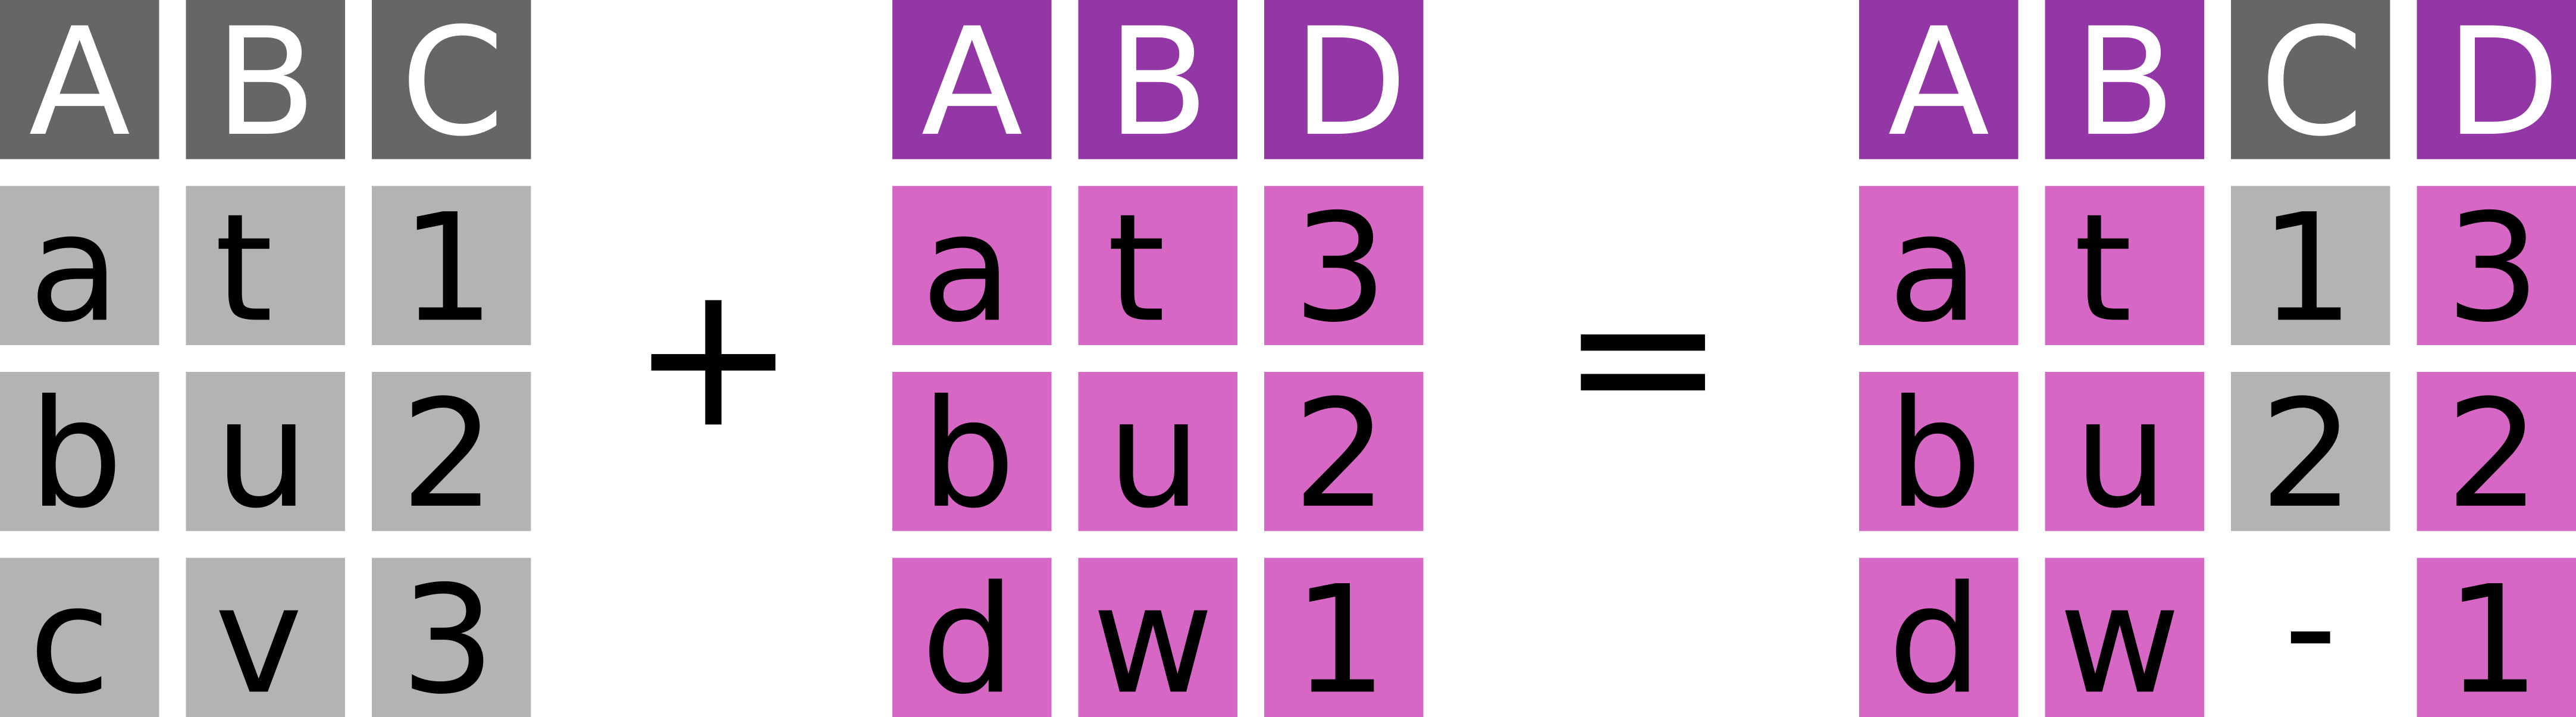
\includegraphics{assets/images/chapters/introduction-to-r/right_join.png}

\begin{Shaded}
\begin{Highlighting}[]
\NormalTok{right }\OtherTok{\textless{}{-}}\NormalTok{ dplyr}\SpecialCharTok{::}\FunctionTok{right\_join}\NormalTok{(}
  \AttributeTok{x =}\NormalTok{ samsub,                           }\CommentTok{\# 1060 observations}
  \AttributeTok{y =}\NormalTok{ libsub,                           }\CommentTok{\# 1657 observations}
  \AttributeTok{by =} \FunctionTok{c}\NormalTok{(}\StringTok{"project\_name"}\NormalTok{, }\StringTok{"sample\_name"}\NormalTok{)}
\NormalTok{)}

\FunctionTok{print}\NormalTok{(right, }\AttributeTok{n =} \DecValTok{1}\NormalTok{)}
\end{Highlighting}
\end{Shaded}

\begin{itemize}
\tightlist
\item
  Right joins are almost identical to left joins -- only x and y have
  reversed roles
\end{itemize}

\hypertarget{inner-join}{%
\subsection{Inner join}\label{inner-join}}

Join the overlapping observations from x and y

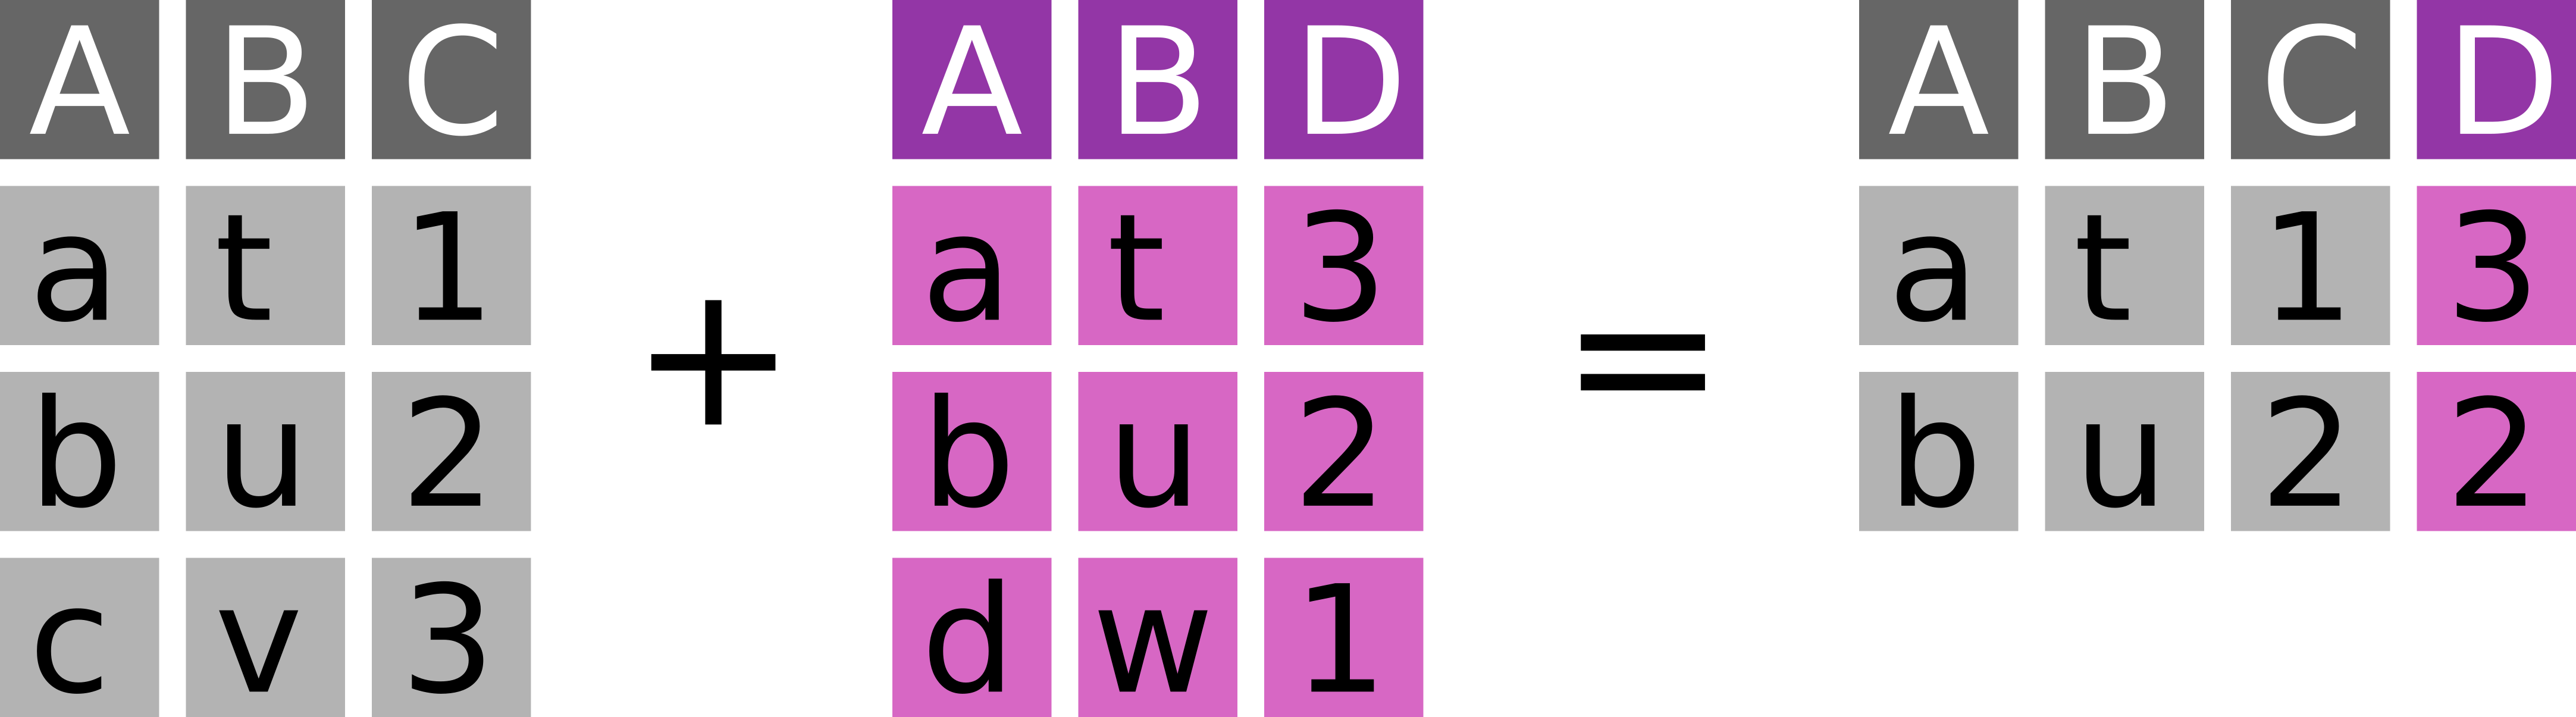
\includegraphics{assets/images/chapters/introduction-to-r/inner_join.png}

\begin{Shaded}
\begin{Highlighting}[]
\NormalTok{inner }\OtherTok{\textless{}{-}}\NormalTok{ dplyr}\SpecialCharTok{::}\FunctionTok{inner\_join}\NormalTok{(}
\AttributeTok{x =}\NormalTok{ samsub,                           }\CommentTok{\# 1060 observations}
\AttributeTok{y =}\NormalTok{ libsub,                           }\CommentTok{\# 1657 observations}
\AttributeTok{by =} \FunctionTok{c}\NormalTok{(}\StringTok{"project\_name"}\NormalTok{, }\StringTok{"sample\_name"}\NormalTok{)}
\NormalTok{)}

\FunctionTok{print}\NormalTok{(inner, }\AttributeTok{n =} \DecValTok{1}\NormalTok{)}
\end{Highlighting}
\end{Shaded}

\begin{itemize}
\tightlist
\item
  Inner joins are a fast and easy way to check, to which degree two
  dataset overlap
\end{itemize}

\hypertarget{full-join}{%
\subsection{Full join}\label{full-join}}

Join all observations from x and y, even if information is missing

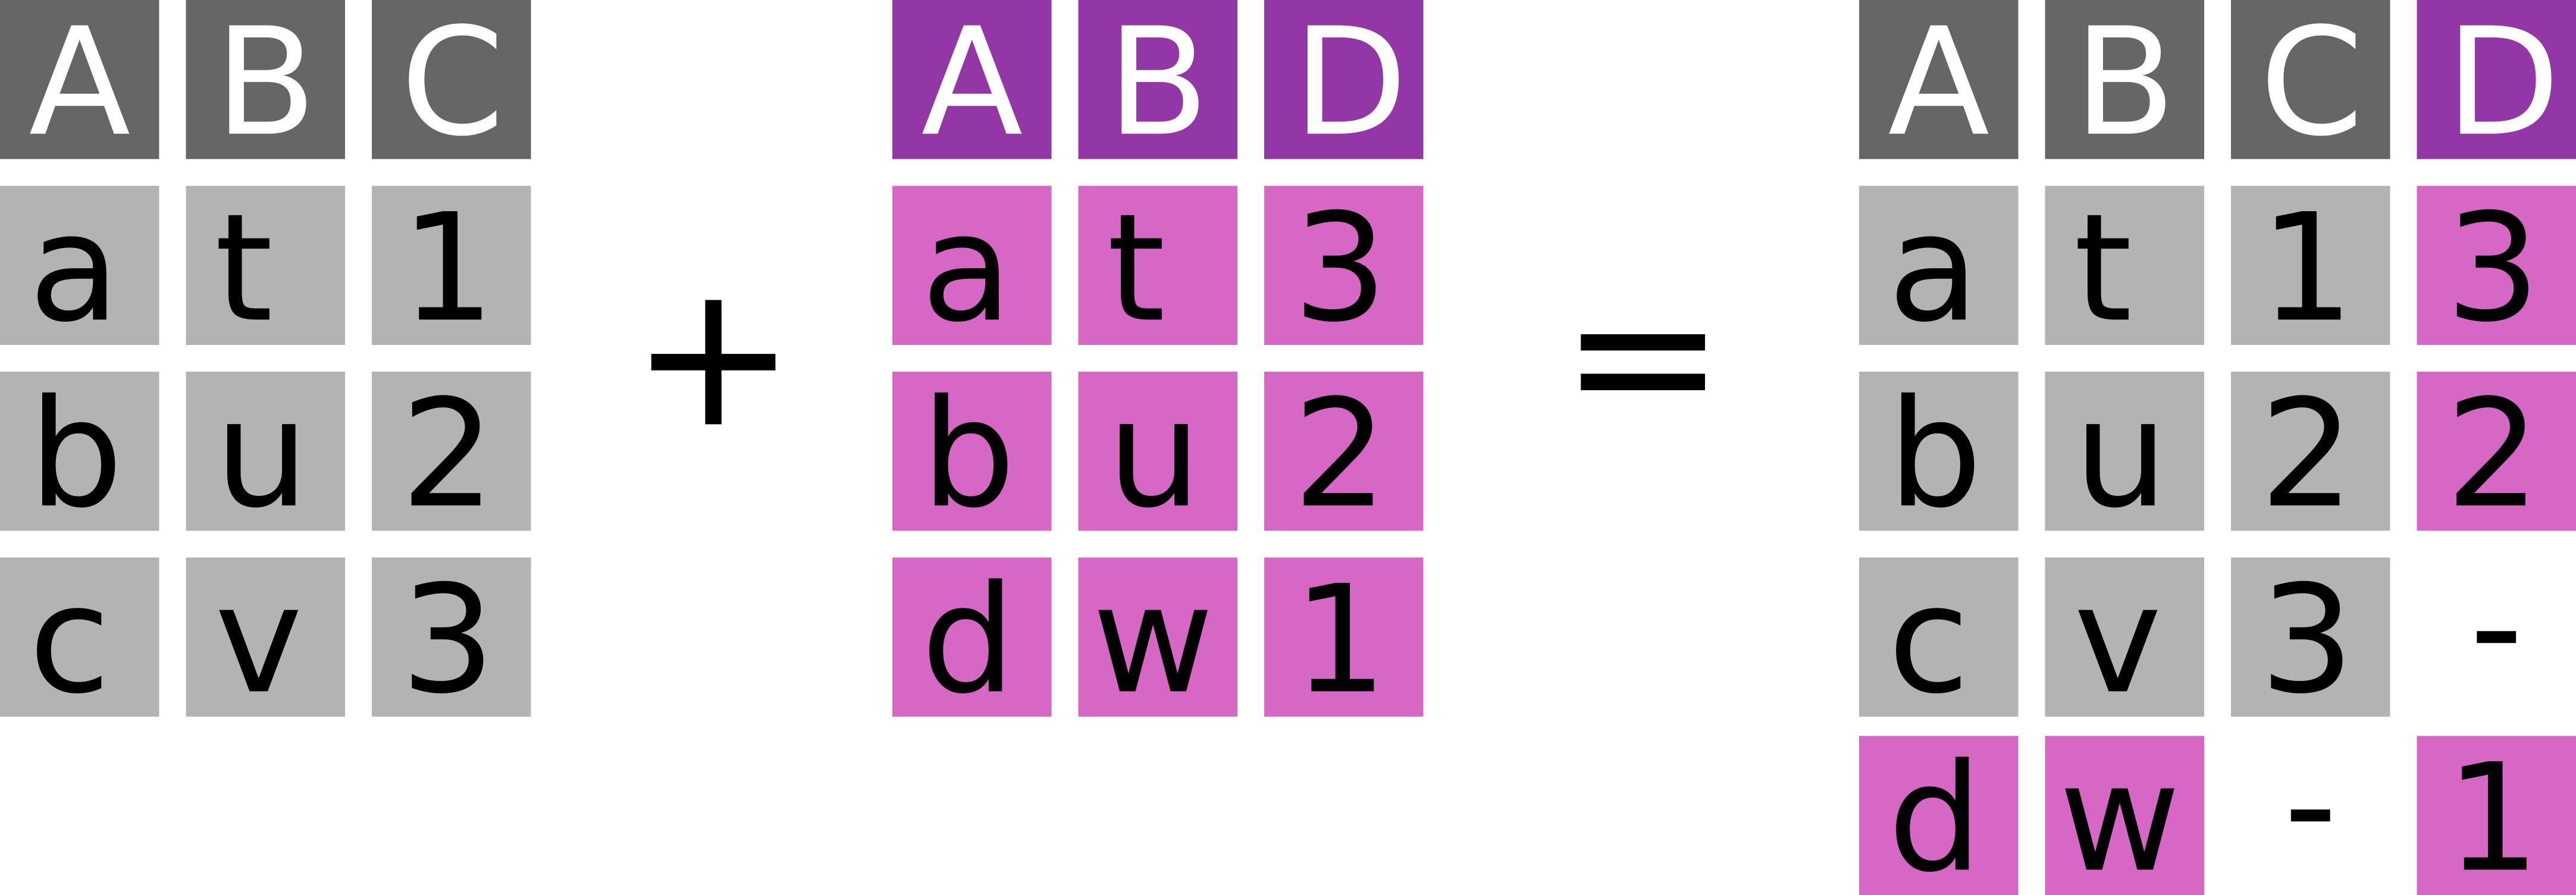
\includegraphics{assets/images/chapters/introduction-to-r/full_join.png}

\begin{Shaded}
\begin{Highlighting}[]
\NormalTok{full }\OtherTok{\textless{}{-}}\NormalTok{ dplyr}\SpecialCharTok{::}\FunctionTok{full\_join}\NormalTok{(}
  \AttributeTok{x =}\NormalTok{ samsub,                           }\CommentTok{\# 1060 observations}
  \AttributeTok{y =}\NormalTok{ libsub,                           }\CommentTok{\# 1657 observations}
  \AttributeTok{by =} \FunctionTok{c}\NormalTok{(}\StringTok{"project\_name"}\NormalTok{, }\StringTok{"sample\_name"}\NormalTok{)}
\NormalTok{)}

\FunctionTok{print}\NormalTok{(full, }\AttributeTok{n =} \DecValTok{1}\NormalTok{)}
\end{Highlighting}
\end{Shaded}

\begin{itemize}
\tightlist
\item
  Full joins allow to preserve every bit of information
\end{itemize}

\hypertarget{semi-join}{%
\subsection{Semi join}\label{semi-join}}

Keep every observation in x that is in y

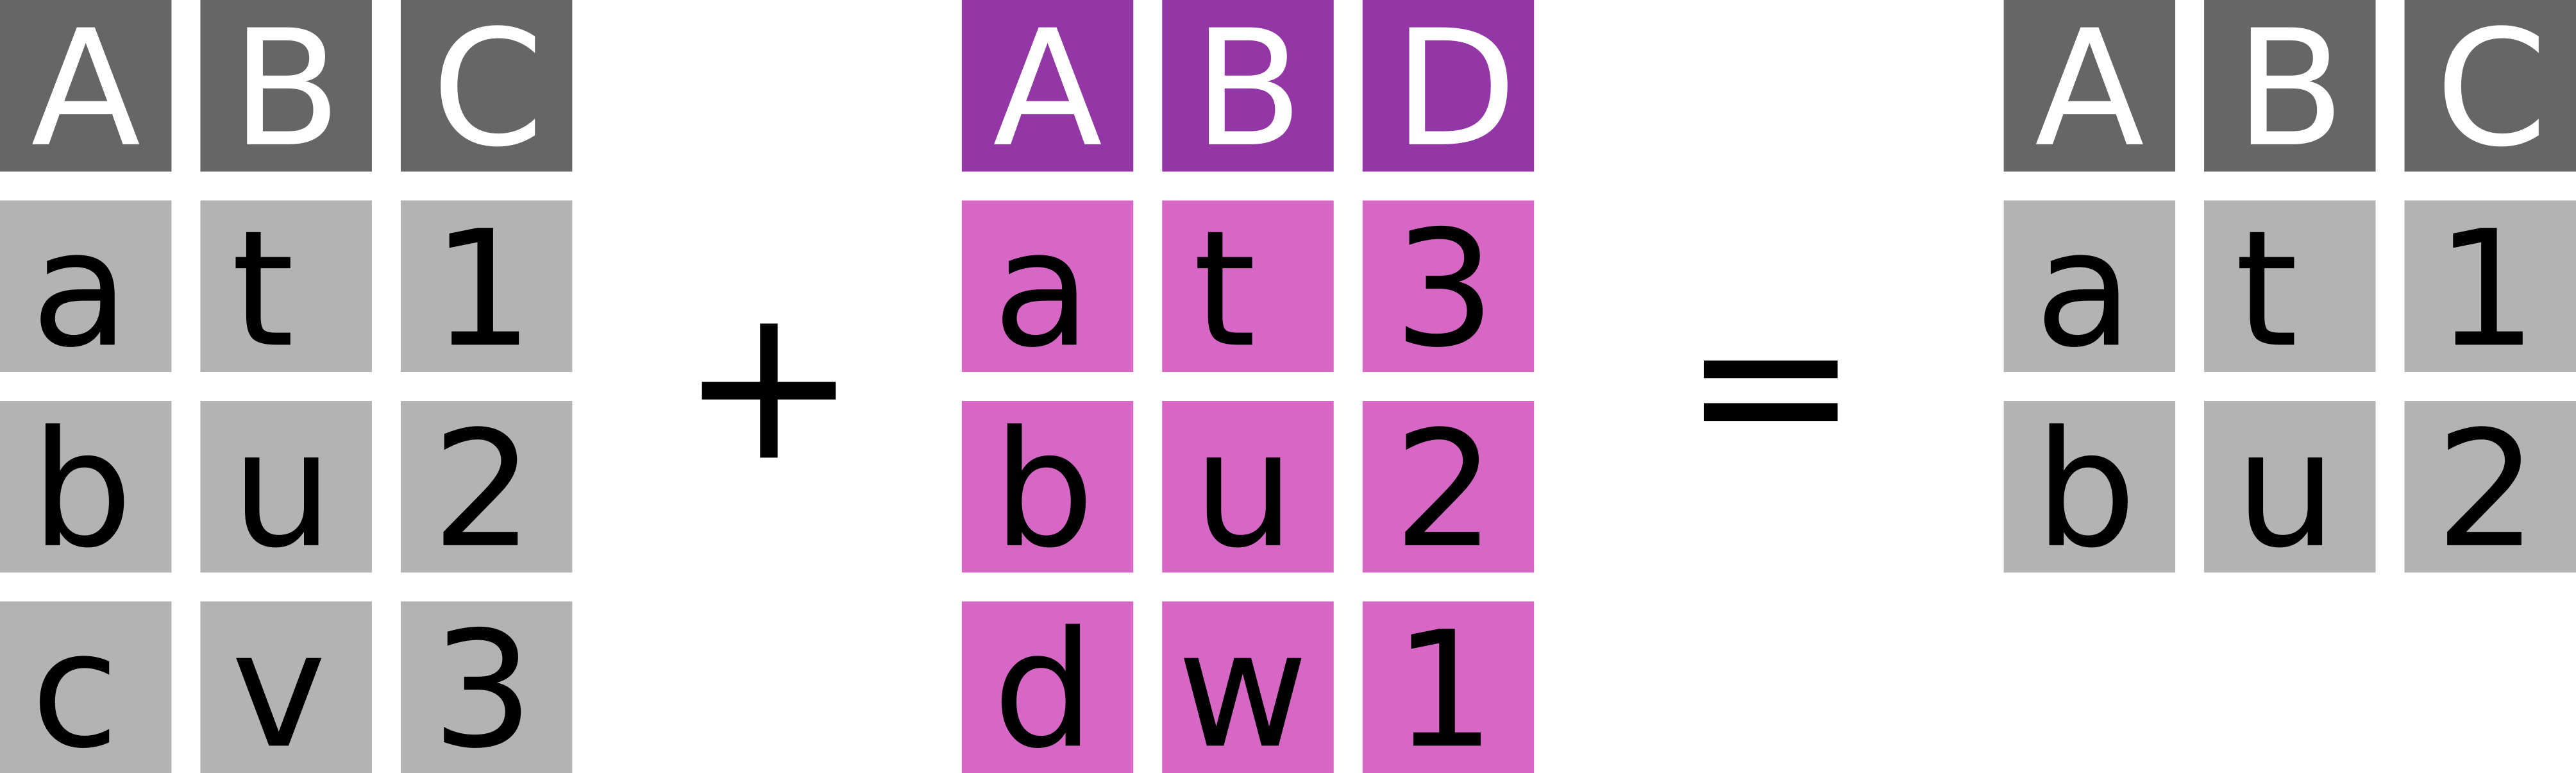
\includegraphics{assets/images/chapters/introduction-to-r/semi_join.png}

\begin{Shaded}
\begin{Highlighting}[]
\NormalTok{semi }\OtherTok{\textless{}{-}}\NormalTok{ dplyr}\SpecialCharTok{::}\FunctionTok{semi\_join}\NormalTok{(}
  \AttributeTok{x =}\NormalTok{ samsub,                           }\CommentTok{\# 1060 observations}
  \AttributeTok{y =}\NormalTok{ libsub,                           }\CommentTok{\# 1657 observations}
  \AttributeTok{by =} \FunctionTok{c}\NormalTok{(}\StringTok{"project\_name"}\NormalTok{, }\StringTok{"sample\_name"}\NormalTok{)}
\NormalTok{)}
\end{Highlighting}
\end{Shaded}

\begin{Shaded}
\begin{Highlighting}[]
\FunctionTok{print}\NormalTok{(semi, }\AttributeTok{n =} \DecValTok{1}\NormalTok{)}
\end{Highlighting}
\end{Shaded}

\begin{itemize}
\tightlist
\item
  Semi joins are underused operations to filter datasets
\end{itemize}

\hypertarget{anti-join}{%
\subsection{Anti join}\label{anti-join}}

Keep every observation in x that is not in y

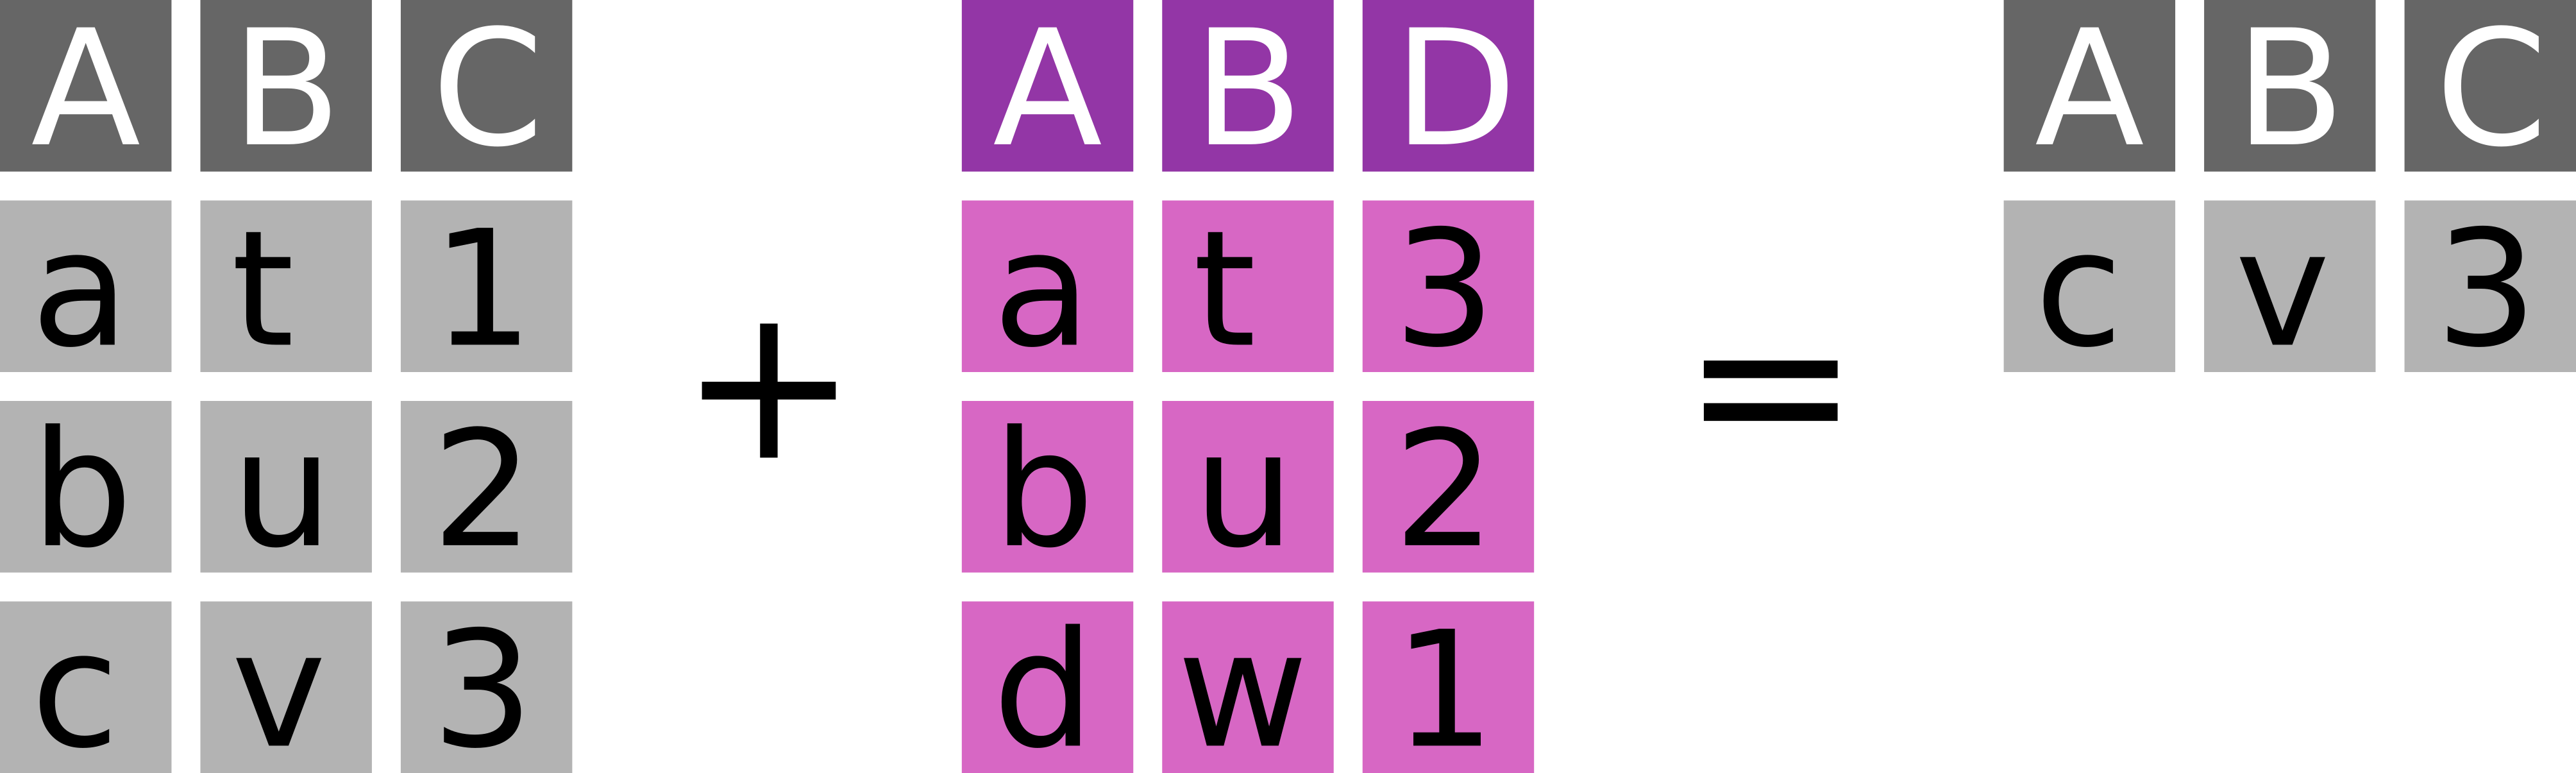
\includegraphics{assets/images/chapters/introduction-to-r/anti_join.png}

\begin{Shaded}
\begin{Highlighting}[]
\NormalTok{anti }\OtherTok{\textless{}{-}}\NormalTok{ dplyr}\SpecialCharTok{::}\FunctionTok{anti\_join}\NormalTok{(}
  \AttributeTok{x =}\NormalTok{ samsub,                           }\CommentTok{\# 1060 observations}
  \AttributeTok{y =}\NormalTok{ libsub,                           }\CommentTok{\# 1657 observations}
  \AttributeTok{by =} \FunctionTok{c}\NormalTok{(}\StringTok{"project\_name"}\NormalTok{, }\StringTok{"sample\_name"}\NormalTok{)}
\NormalTok{)}
\end{Highlighting}
\end{Shaded}

\begin{Shaded}
\begin{Highlighting}[]
\FunctionTok{print}\NormalTok{(anti, }\AttributeTok{n =} \DecValTok{1}\NormalTok{)}
\end{Highlighting}
\end{Shaded}

\begin{itemize}
\tightlist
\item
  Anti joins allow to quickly specify incomplete datasets and missing
  information
\end{itemize}

\hypertarget{exercise-4}{%
\subsection{Exercise 4}\label{exercise-4}}

Consider the following additional dataset:

\begin{Shaded}
\begin{Highlighting}[]
\NormalTok{gear\_opinions }\OtherTok{\textless{}{-}}\NormalTok{ tibble}\SpecialCharTok{::}\FunctionTok{tibble}\NormalTok{(}\AttributeTok{gear =} \FunctionTok{c}\NormalTok{(}\DecValTok{3}\NormalTok{, }\DecValTok{5}\NormalTok{), }\AttributeTok{opinion =} \FunctionTok{c}\NormalTok{(}\StringTok{"boring"}\NormalTok{, }\StringTok{"wow"}\NormalTok{))}
\end{Highlighting}
\end{Shaded}

\begin{enumerate}
\def\labelenumi{\arabic{enumi}.}
\item
  Add my opinions about gears to the \texttt{mtcars} dataset

\begin{Shaded}
\begin{Highlighting}[]

\end{Highlighting}
\end{Shaded}
\item
  Remove all cars from the dataset for which I don't have an opinion

\begin{Shaded}
\begin{Highlighting}[]

\end{Highlighting}
\end{Shaded}
\end{enumerate}

\hypertarget{possible-solutions-4}{%
\subsection{Possible Solutions 4}\label{possible-solutions-4}}

\begin{enumerate}
\def\labelenumi{\arabic{enumi}.}
\item
  Add my opinions about gears to the \texttt{mtcars} dataset

\begin{Shaded}
\begin{Highlighting}[]
\NormalTok{dplyr}\SpecialCharTok{::}\FunctionTok{left\_join}\NormalTok{(mtcars, gear\_opinions, }\AttributeTok{by =} \StringTok{"gear"}\NormalTok{)}
\end{Highlighting}
\end{Shaded}
\item
  Remove all cars from the dataset for which I don't have an opinion

\begin{Shaded}
\begin{Highlighting}[]
\NormalTok{dplyr}\SpecialCharTok{::}\FunctionTok{anti\_join}\NormalTok{(mtcars, gear\_opinions, }\AttributeTok{by =} \StringTok{"gear"}\NormalTok{)}
\end{Highlighting}
\end{Shaded}
\end{enumerate}

\hypertarget{introduction-to-python-and-pandas}{%
\chapter{Introduction to Python and
Pandas}\label{introduction-to-python-and-pandas}}

\begin{tcolorbox}[enhanced jigsaw, opacitybacktitle=0.6, bottomtitle=1mm, opacityback=0, colback=white, coltitle=black, leftrule=.75mm, toprule=.15mm, title=\textcolor{quarto-callout-note-color}{\faInfo}\hspace{0.5em}{Note}, colframe=quarto-callout-note-color-frame, toptitle=1mm, arc=.35mm, left=2mm, titlerule=0mm, breakable, rightrule=.15mm, bottomrule=.15mm, colbacktitle=quarto-callout-note-color!10!white]

This session is typically ran held in parallel to the Introduction to R
and Tidyverse. Participants of the summer schools chose which to attend
based on their prior experience. We recommend the introduction to R
session if you have no experience with neither R nor Python.

\end{tcolorbox}

\begin{tcolorbox}[enhanced jigsaw, opacitybacktitle=0.6, bottomtitle=1mm, opacityback=0, colback=white, coltitle=black, leftrule=.75mm, toprule=.15mm, title=\textcolor{quarto-callout-tip-color}{\faLightbulb}\hspace{0.5em}{Tip}, colframe=quarto-callout-tip-color-frame, toptitle=1mm, arc=.35mm, left=2mm, titlerule=0mm, breakable, rightrule=.15mm, bottomrule=.15mm, colbacktitle=quarto-callout-tip-color!10!white]

For this chapter's exercises, if not already performed, you will need to
create the \protect\hyperlink{creating-a-conda-environment}{conda
environment} from the \texttt{yml} file in the following
\href{https://doi.org/10.5281/zenodo.6983159}{archive}, and activate the
environment:

\begin{Shaded}
\begin{Highlighting}[]
\ExtensionTok{conda}\NormalTok{ activate r{-}python}
\end{Highlighting}
\end{Shaded}

\end{tcolorbox}

\hypertarget{lecture-7}{%
\section{Lecture}\label{lecture-7}}

PDF version of these slides can be downloaded from
\href{https://github.com/SPAAM-community/wss-summer-school/raw/main/docs/assets/slides/2022/3b2-python-pandas/SPAAM\%20Summer\%20School\%202022\%20-\%203B2\%20-\%20Intro\%20to\%20Python\%20and\%20Pandas.pdf}{here}.

This session is run using a Jupyter notebook. This can be found
\href{https://github.com/maxibor/intro-to-pandas-plotnine}{here}.
However, it will already be installed on compute nodes during the summer
school.

\begin{tcolorbox}[enhanced jigsaw, opacitybacktitle=0.6, bottomtitle=1mm, opacityback=0, colback=white, coltitle=black, leftrule=.75mm, toprule=.15mm, title=\textcolor{quarto-callout-warning-color}{\faExclamationTriangle}\hspace{0.5em}{Warning}, colframe=quarto-callout-warning-color-frame, toptitle=1mm, arc=.35mm, left=2mm, titlerule=0mm, breakable, rightrule=.15mm, bottomrule=.15mm, colbacktitle=quarto-callout-warning-color!10!white]

We highly recommend viewing this walkthrough via the Jupyter notebook
above! The output of commands on the website for this walkthrough are
displayed in their own code blocks - be wary of what you copy-paste!

\end{tcolorbox}

\begin{Shaded}
\begin{Highlighting}[]
\ImportTok{from}\NormalTok{ IPython.core.display }\ImportTok{import}\NormalTok{ SVG}
\end{Highlighting}
\end{Shaded}

\hypertarget{introduction-to-data-manipulation-in-python-with-pandas-and-visulization-with-plotnine}{%
\section{Introduction to data manipulation in Python with Pandas and
visulization with
plotnine}\label{introduction-to-data-manipulation-in-python-with-pandas-and-visulization-with-plotnine}}

Maxime Borry\\
SPAAM Summer School 2022

\begin{Shaded}
\begin{Highlighting}[]
\NormalTok{SVG(filename}\OperatorTok{=}\StringTok{\textquotesingle{}img/whoami.svg\textquotesingle{}}\NormalTok{)}
\end{Highlighting}
\end{Shaded}

\begin{figure}

{\centering 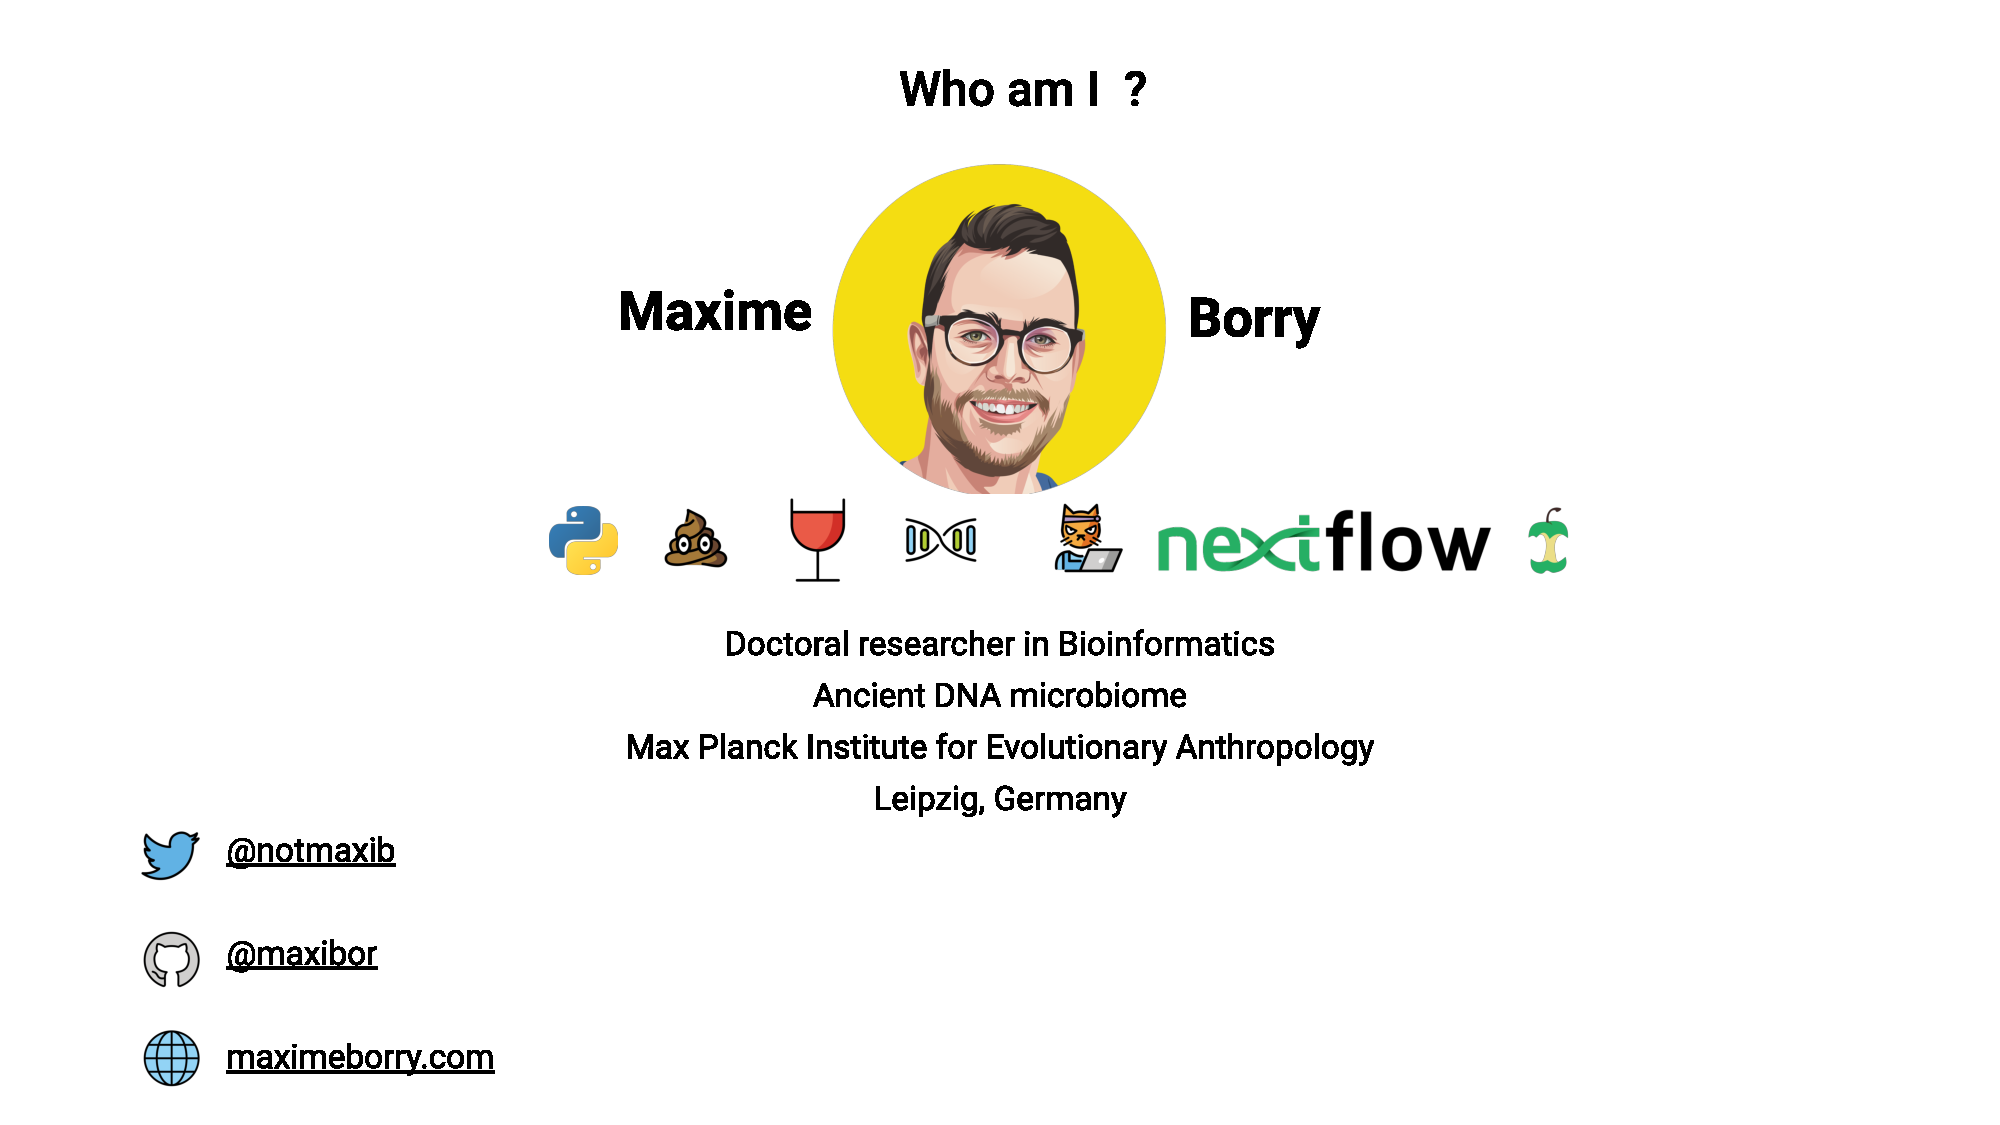
\includegraphics{index_files/mediabag/assets/images/chapters/introduction-to-python/tutorial_2_0.pdf}

}

\caption{svg}

\end{figure}

Over the last few years, Python has gained an immense amount of
popularity thanks to its numerous libraries in the field of machine
learning, statistical data analysis, and bioinformatics. While a few
years ago, it was often necessary to go back to R for performing routine
data manipulation and analysis tasks, nowadays Python has a vast
ecosystem of libraries for doing just that.

Today, we will do a quick introduction of the most popular libraries for
data analysis:

\begin{itemize}
\tightlist
\item
  \href{https://pandas.pydata.org/}{pandas}, for reading and
  manipulation tabular data
\item
  \href{https://plotnine.readthedocs.io/}{plotnine}, the Python clone of
  ggplot2
\end{itemize}

\hypertarget{overview}{%
\section{Overview:}\label{overview}}

\begin{itemize}
\tightlist
\item
  0 - Foreword, working in a jupyter environment
\item
  1 - Loading required libraries
\item
  2 - Foreword on Pandas
\item
  3 - Reading data with Pandas
\item
  4 - Dealing with missing data
\item
  5 - Computing basic statistics
\item
  6 - Filtering
\item
  8 - GroupBy operations
\item
  9 - Joining different tables
\item
  10 - Visualization with Plotnine
\end{itemize}

\hypertarget{foreword-working-in-a-jupyter-environment}{%
\section{0 - Foreword, working in a jupyter
environment}\label{foreword-working-in-a-jupyter-environment}}

\hypertarget{this-is-a-markdown-cell}{%
\subsection{This is a markdown cell}\label{this-is-a-markdown-cell}}

With some features of the markdown syntax, such as:

\begin{itemize}
\tightlist
\item
  \textbf{bold} \texttt{**bold**}
\item
  \emph{italic} \texttt{*italic*}
\item
  \texttt{inline\ code}
\end{itemize}

\begin{verbatim}
`inline code`
\end{verbatim}

\begin{itemize}
\item
  \href{https://www.google.com/}{links}
  \texttt{{[}links{]}(https://www.google.com/)}
\item
  Images\\
  
\includegraphics{assets/images/chapters/introduction-to-python/avatar_hu4dc3c23d5a8c195732bbca11d7ce61be_114670_270x270_fill_lanczos_center_2.png}\\
  \texttt{!{[}{]}(https://maximeborry.com/authors/maxime/avatar\_hu4dc3c23d5a8c195732bbca11d7ce61be\_114670\_270x270\_fill\_lanczos\_center\_2.png)}
\item
  Latex code \$ y = ax + b\$\\
  \texttt{\$y\ =\ ax\ +\ b\$}
\end{itemize}

\begin{Shaded}
\begin{Highlighting}[]
\BuiltInTok{print}\NormalTok{(}\StringTok{"This is a code cell in Python"}\NormalTok{)}
\end{Highlighting}
\end{Shaded}

\begin{verbatim}
This is a code cell in Python
\end{verbatim}

\begin{Shaded}
\begin{Highlighting}[]
\OperatorTok{!}\NormalTok{ echo }\StringTok{"This is code cell in bash"}
\end{Highlighting}
\end{Shaded}

\begin{verbatim}
This is code cell in bash
\end{verbatim}

\begin{Shaded}
\begin{Highlighting}[]
\ExtensionTok{\%\%bash}

\BuiltInTok{echo} \StringTok{"This a multiline code cell"}
\BuiltInTok{echo} \StringTok{"in bash"}
\end{Highlighting}
\end{Shaded}

\begin{verbatim}
This a multiline code cell
in bash
\end{verbatim}

\hypertarget{loading-required-libraries}{%
\section{1 - Loading required
libraries}\label{loading-required-libraries}}

\begin{Shaded}
\begin{Highlighting}[]
\ImportTok{import}\NormalTok{ pandas }\ImportTok{as}\NormalTok{ pd}
\ImportTok{import}\NormalTok{ numpy }\ImportTok{as}\NormalTok{ np}
\ImportTok{from}\NormalTok{ plotnine }\ImportTok{import} \OperatorTok{*}
\end{Highlighting}
\end{Shaded}

\begin{Shaded}
\begin{Highlighting}[]
\NormalTok{pd.\_\_version\_\_}
\end{Highlighting}
\end{Shaded}

\begin{verbatim}
'1.4.3'
\end{verbatim}

\begin{Shaded}
\begin{Highlighting}[]
\NormalTok{np.\_\_version\_\_}
\end{Highlighting}
\end{Shaded}

\begin{verbatim}
'1.23.1'
\end{verbatim}

\begin{Shaded}
\begin{Highlighting}[]
\OperatorTok{!}\NormalTok{ conda }\BuiltInTok{list} \OperatorTok{|}\NormalTok{ grep plotnine}
\end{Highlighting}
\end{Shaded}

\begin{verbatim}
plotnine                  0.9.0              pyhd8ed1ab_0    conda-forge
\end{verbatim}

\hypertarget{foreword-on-pandas}{%
\section{2 - Foreword on Pandas}\label{foreword-on-pandas}}

\hypertarget{pandas-terminology}{%
\subsection{Pandas terminology}\label{pandas-terminology}}

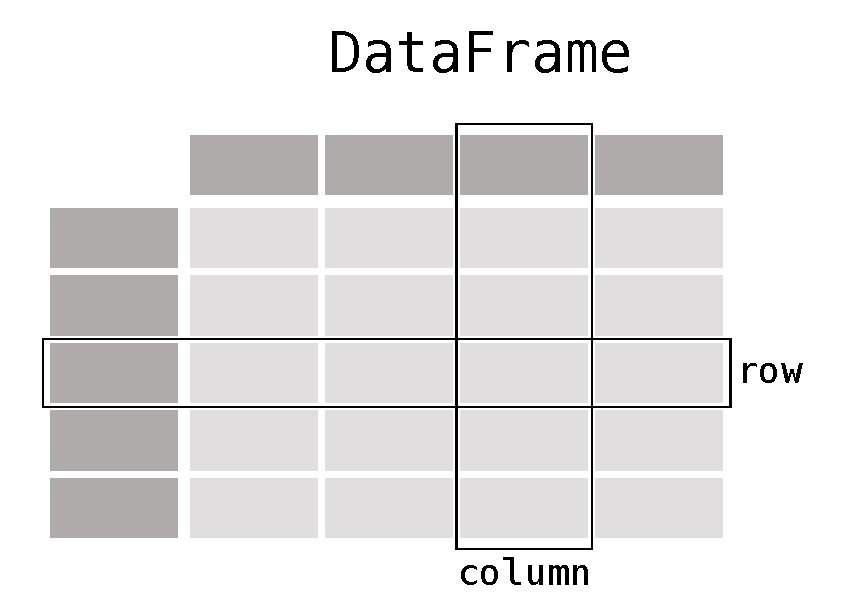
\includegraphics{index_files/mediabag/assets/images/chapters/introduction-to-python/01_table_dataframe.pdf}

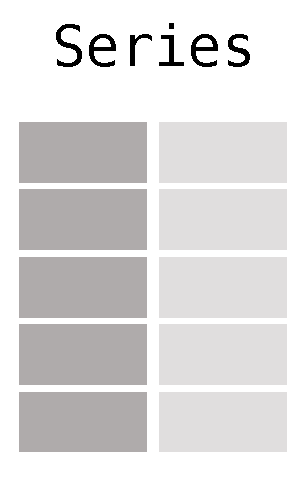
\includegraphics{index_files/mediabag/assets/images/chapters/introduction-to-python/01_table_series.pdf}

The pandas getting started tutorial:
\href{https://pandas.pydata.org/docs/getting_started/index.html\#}{pandas.pydata.org/docs/getting\_started}

\hypertarget{reading-data-with-pandas}{%
\section{3 - Reading data with Pandas}\label{reading-data-with-pandas}}

\begin{Shaded}
\begin{Highlighting}[]
\NormalTok{sample\_table\_url }\OperatorTok{=} \StringTok{"https://raw.githubusercontent.com/SPAAM{-}community/AncientMetagenomeDir/b187df6ebd23dfeb42935fd5020cb615ead3f164/}
\ErrorTok{ancientmetagenome{-}hostassociated/samples/ancientmetagenome{-}hostassociated\_samples.tsv"}
\NormalTok{library\_table\_url }\OperatorTok{=} \StringTok{"https://raw.githubusercontent.com/SPAAM{-}community/AncientMetagenomeDir/b187df6ebd23dfeb42935fd5020cb615ead3f164/}
\ErrorTok{ancientmetagenome{-}hostassociated/libraries/ancientmetagenome{-}hostassociated\_libraries.tsv"}
\end{Highlighting}
\end{Shaded}

Getting help in Python

\begin{Shaded}
\begin{Highlighting}[]
\BuiltInTok{help}\NormalTok{(pd.read\_csv)}
\end{Highlighting}
\end{Shaded}

\begin{verbatim}
Help on function read_csv in module pandas.io.parsers.readers:

read_csv(filepath_or_buffer: 'FilePath | ReadCsvBuffer[bytes] | ReadCsvBuffer[str]',
sep=<no_default>, delimiter=None, header='infer', names=<no_default>, index_col=None,
usecols=None, squeeze=None, prefix=<no_default>, mangle_dupe_cols=True,
dtype: 'DtypeArg | None' = None, engine: 'CSVEngine | None' = None, converters=None,
true_values=None, false_values=None, skipinitialspace=False, skiprows=None, skipfooter=0,
nrows=None, na_values=None, keep_default_na=True, na_filter=True, verbose=False,
skip_blank_lines=True, parse_dates=None, infer_datetime_format=False, keep_date_col=False,
 date_parser=None, dayfirst=False, cache_dates=True, iterator=False, chunksize=None,
 compression: 'CompressionOptions' = 'infer', thousands=None, decimal: 'str' = '.',
 lineterminator=None, quotechar='"', quoting=0, doublequote=True, escapechar=None,
 comment=None, encoding=None, encoding_errors: 'str | None' = 'strict', dialect=None,
 error_bad_lines=None, warn_bad_lines=None, on_bad_lines=None, delim_whitespace=False,
 low_memory=True, memory_map=False, float_precision=None, storage_options: 'StorageOptions' = None)
    Read a comma-separated values (csv) file into DataFrame.

    Also supports optionally iterating or breaking of the file
    into chunks.

    Additional help can be found in the online docs for
    `IO Tools <https://pandas.pydata.org/pandas-docs/stable/user_guide/io.html>`_.

    Parameters
    ----------
    filepath_or_buffer : str, path object or file-like object
        Any valid string path is acceptable. The string could be a URL. Valid
        URL schemes include http, ftp, s3, gs, and file. For file URLs, a host is
        expected. A local file could be: file://localhost/path/to/table.csv.

        If you want to pass in a path object, pandas accepts any ``os.PathLike``.

        By file-like object, we refer to objects with a ``read()`` method, such as
        a file handle (e.g. via builtin ``open`` function) or ``StringIO``.
    sep : str, default ','
        Delimiter to use. If sep is None, the C engine cannot automatically detect
        the separator, but the Python parsing engine can, meaning the latter will
        be used and automatically detect the separator by Python's builtin sniffer
        tool, ``csv.Sniffer``. In addition, separators longer than 1 character and
        different from ``'\s+'`` will be interpreted as regular expressions and
        will also force the use of the Python parsing engine. Note that regex
        delimiters are prone to ignoring quoted data. Regex example: ``'\r\t'``.
    delimiter : str, default ``None``
        Alias for sep.
    header : int, list of int, None, default 'infer'
        Row number(s) to use as the column names, and the start of the
        data.  Default behavior is to infer the column names: if no names
        are passed the behavior is identical to ``header=0`` and column
        names are inferred from the first line of the file, if column
        names are passed explicitly then the behavior is identical to
        ``header=None``. Explicitly pass ``header=0`` to be able to
        replace existing names. The header can be a list of integers that
        specify row locations for a multi-index on the columns
        e.g. [0,1,3]. Intervening rows that are not specified will be
        skipped (e.g. 2 in this example is skipped). Note that this
        parameter ignores commented lines and empty lines if
        ``skip_blank_lines=True``, so ``header=0`` denotes the first line of
        data rather than the first line of the file.
    names : array-like, optional
        List of column names to use. If the file contains a header row,
        then you should explicitly pass ``header=0`` to override the column names.
        Duplicates in this list are not allowed.
    index_col : int, str, sequence of int / str, or False, optional, default ``None``
      Column(s) to use as the row labels of the ``DataFrame``, either given as
      string name or column index. If a sequence of int / str is given, a
      MultiIndex is used.

      Note: ``index_col=False`` can be used to force pandas to *not* use the first
      column as the index, e.g. when you have a malformed file with delimiters at
      the end of each line.
    usecols : list-like or callable, optional
        Return a subset of the columns. If list-like, all elements must either
        be positional (i.e. integer indices into the document columns) or strings
        that correspond to column names provided either by the user in `names` or
        inferred from the document header row(s). If ``names`` are given, the document
        header row(s) are not taken into account. For example, a valid list-like
        `usecols` parameter would be ``[0, 1, 2]`` or ``['foo', 'bar', 'baz']``.
        Element order is ignored, so ``usecols=[0, 1]`` is the same as ``[1, 0]``.
        To instantiate a DataFrame from ``data`` with element order preserved use
        ``pd.read_csv(data, usecols=['foo', 'bar'])[['foo', 'bar']]`` for columns
        in ``['foo', 'bar']`` order or
        ``pd.read_csv(data, usecols=['foo', 'bar'])[['bar', 'foo']]``
        for ``['bar', 'foo']`` order.

        If callable, the callable function will be evaluated against the column
        names, returning names where the callable function evaluates to True. An
        example of a valid callable argument would be ``lambda x: x.upper() in
        ['AAA', 'BBB', 'DDD']``. Using this parameter results in much faster
        parsing time and lower memory usage.
    squeeze : bool, default False
        If the parsed data only contains one column then return a Series.

        .. deprecated:: 1.4.0
            Append ``.squeeze("columns")`` to the call to ``read_csv`` to squeeze
            the data.
    prefix : str, optional
        Prefix to add to column numbers when no header, e.g. 'X' for X0, X1, ...

        .. deprecated:: 1.4.0
           Use a list comprehension on the DataFrame's columns after calling ``read_csv``.
    mangle_dupe_cols : bool, default True
        Duplicate columns will be specified as 'X', 'X.1', ...'X.N', rather than
        'X'...'X'. Passing in False will cause data to be overwritten if there
        are duplicate names in the columns.
    dtype : Type name or dict of column -> type, optional
        Data type for data or columns. E.g. {'a': np.float64, 'b': np.int32,
        'c': 'Int64'}
        Use `str` or `object` together with suitable `na_values` settings
        to preserve and not interpret dtype.
        If converters are specified, they will be applied INSTEAD
        of dtype conversion.
    engine : {'c', 'python', 'pyarrow'}, optional
        Parser engine to use. The C and pyarrow engines are faster, while the python engine
        is currently more feature-complete. Multithreading is currently only supported by
        the pyarrow engine.

        .. versionadded:: 1.4.0

            The "pyarrow" engine was added as an *experimental* engine, and some features
            are unsupported, or may not work correctly, with this engine.
    converters : dict, optional
        Dict of functions for converting values in certain columns. Keys can either
        be integers or column labels.
    true_values : list, optional
        Values to consider as True.
    false_values : list, optional
        Values to consider as False.
    skipinitialspace : bool, default False
        Skip spaces after delimiter.
    skiprows : list-like, int or callable, optional
        Line numbers to skip (0-indexed) or number of lines to skip (int)
        at the start of the file.

        If callable, the callable function will be evaluated against the row
        indices, returning True if the row should be skipped and False otherwise.
        An example of a valid callable argument would be ``lambda x: x in [0, 2]``.
    skipfooter : int, default 0
        Number of lines at bottom of file to skip (Unsupported with engine='c').
    nrows : int, optional
        Number of rows of file to read. Useful for reading pieces of large files.
    na_values : scalar, str, list-like, or dict, optional
        Additional strings to recognize as NA/NaN. If dict passed, specific
        per-column NA values.  By default the following values are interpreted as
        NaN: '', '#N/A', '#N/A N/A', '#NA', '-1.#IND', '-1.#QNAN', '-NaN', '-nan',
        '1.#IND', '1.#QNAN', '<NA>', 'N/A', 'NA', 'NULL', 'NaN', 'n/a',
        'nan', 'null'.
    keep_default_na : bool, default True
        Whether or not to include the default NaN values when parsing the data.
        Depending on whether `na_values` is passed in, the behavior is as follows:

        * If `keep_default_na` is True, and `na_values` are specified, `na_values`
          is appended to the default NaN values used for parsing.
        * If `keep_default_na` is True, and `na_values` are not specified, only
          the default NaN values are used for parsing.
        * If `keep_default_na` is False, and `na_values` are specified, only
          the NaN values specified `na_values` are used for parsing.
        * If `keep_default_na` is False, and `na_values` are not specified, no
          strings will be parsed as NaN.

        Note that if `na_filter` is passed in as False, the `keep_default_na` and
        `na_values` parameters will be ignored.
    na_filter : bool, default True
        Detect missing value markers (empty strings and the value of na_values). In
        data without any NAs, passing na_filter=False can improve the performance
        of reading a large file.
    verbose : bool, default False
        Indicate number of NA values placed in non-numeric columns.
    skip_blank_lines : bool, default True
        If True, skip over blank lines rather than interpreting as NaN values.
    parse_dates : bool or list of int or names or list of lists or dict, default False
        The behavior is as follows:

        * boolean. If True -> try parsing the index.
        * list of int or names. e.g. If [1, 2, 3] -> try parsing columns 1, 2, 3
          each as a separate date column.
        * list of lists. e.g.  If [[1, 3]] -> combine columns 1 and 3 and parse as
          a single date column.
        * dict, e.g. {'foo' : [1, 3]} -> parse columns 1, 3 as date and call
          result 'foo'

        If a column or index cannot be represented as an array of datetimes,
        say because of an unparsable value or a mixture of timezones, the column
        or index will be returned unaltered as an object data type. For
        non-standard datetime parsing, use ``pd.to_datetime`` after
        ``pd.read_csv``. To parse an index or column with a mixture of timezones,
        specify ``date_parser`` to be a partially-applied
        :func:`pandas.to_datetime` with ``utc=True``. See
        :ref:`io.csv.mixed_timezones` for more.

        Note: A fast-path exists for iso8601-formatted dates.
    infer_datetime_format : bool, default False
        If True and `parse_dates` is enabled, pandas will attempt to infer the
        format of the datetime strings in the columns, and if it can be inferred,
        switch to a faster method of parsing them. In some cases this can increase
        the parsing speed by 5-10x.
    keep_date_col : bool, default False
        If True and `parse_dates` specifies combining multiple columns then
        keep the original columns.
    date_parser : function, optional
        Function to use for converting a sequence of string columns to an array of
        datetime instances. The default uses ``dateutil.parser.parser`` to do the
        conversion. Pandas will try to call `date_parser` in three different ways,
        advancing to the next if an exception occurs: 1) Pass one or more arrays
        (as defined by `parse_dates`) as arguments; 2) concatenate (row-wise) the
        string values from the columns defined by `parse_dates` into a single array
        and pass that; and 3) call `date_parser` once for each row using one or
        more strings (corresponding to the columns defined by `parse_dates`) as
        arguments.
    dayfirst : bool, default False
        DD/MM format dates, international and European format.
    cache_dates : bool, default True
        If True, use a cache of unique, converted dates to apply the datetime
        conversion. May produce significant speed-up when parsing duplicate
        date strings, especially ones with timezone offsets.

        .. versionadded:: 0.25.0
    iterator : bool, default False
        Return TextFileReader object for iteration or getting chunks with
        ``get_chunk()``.

        .. versionchanged:: 1.2

           ``TextFileReader`` is a context manager.
    chunksize : int, optional
        Return TextFileReader object for iteration.
        See the `IO Tools docs
        <https://pandas.pydata.org/pandas-docs/stable/io.html#io-chunking>`_
        for more information on ``iterator`` and ``chunksize``.

        .. versionchanged:: 1.2

           ``TextFileReader`` is a context manager.
    compression : str or dict, default 'infer'
        For on-the-fly decompression of on-disk data. If 'infer' and '%s' is
        path-like, then detect compression from the following extensions: '.gz',
        '.bz2', '.zip', '.xz', or '.zst' (otherwise no compression). If using
        'zip', the ZIP file must contain only one data file to be read in. Set to
        ``None`` for no decompression. Can also be a dict with key ``'method'`` set
        to one of {``'zip'``, ``'gzip'``, ``'bz2'``, ``'zstd'``} and other
        key-value pairs are forwarded to ``zipfile.ZipFile``, ``gzip.GzipFile``,
        ``bz2.BZ2File``, or ``zstandard.ZstdDecompressor``, respectively. As an
        example, the following could be passed for Zstandard decompression using a
        custom compression dictionary:
        ``compression={'method': 'zstd', 'dict_data': my_compression_dict}``.

        .. versionchanged:: 1.4.0 Zstandard support.

    thousands : str, optional
        Thousands separator.
    decimal : str, default '.'
        Character to recognize as decimal point (e.g. use ',' for European data).
    lineterminator : str (length 1), optional
        Character to break file into lines. Only valid with C parser.
    quotechar : str (length 1), optional
        The character used to denote the start and end of a quoted item. Quoted
        items can include the delimiter and it will be ignored.
    quoting : int or csv.QUOTE_* instance, default 0
        Control field quoting behavior per ``csv.QUOTE_*`` constants. Use one of
        QUOTE_MINIMAL (0), QUOTE_ALL (1), QUOTE_NONNUMERIC (2) or QUOTE_NONE (3).
    doublequote : bool, default ``True``
       When quotechar is specified and quoting is not ``QUOTE_NONE``, indicate
       whether or not to interpret two consecutive quotechar elements INSIDE a
       field as a single ``quotechar`` element.
    escapechar : str (length 1), optional
        One-character string used to escape other characters.
    comment : str, optional
        Indicates remainder of line should not be parsed. If found at the beginning
        of a line, the line will be ignored altogether. This parameter must be a
        single character. Like empty lines (as long as ``skip_blank_lines=True``),
        fully commented lines are ignored by the parameter `header` but not by
        `skiprows`. For example, if ``comment='#'``, parsing
        ``#empty\na,b,c\n1,2,3`` with ``header=0`` will result in 'a,b,c' being
        treated as the header.
    encoding : str, optional
        Encoding to use for UTF when reading/writing (ex. 'utf-8'). `List of Python
        standard encodings
        <https://docs.python.org/3/library/codecs.html#standard-encodings>`_ .

        .. versionchanged:: 1.2

           When ``encoding`` is ``None``, ``errors="replace"`` is passed to
           ``open()``. Otherwise, ``errors="strict"`` is passed to ``open()``.
           This behavior was previously only the case for ``engine="python"``.

        .. versionchanged:: 1.3.0

           ``encoding_errors`` is a new argument. ``encoding`` has no longer an
           influence on how encoding errors are handled.

    encoding_errors : str, optional, default "strict"
        How encoding errors are treated. `List of possible values
        <https://docs.python.org/3/library/codecs.html#error-handlers>`_ .

        .. versionadded:: 1.3.0

    dialect : str or csv.Dialect, optional
        If provided, this parameter will override values (default or not) for the
        following parameters: `delimiter`, `doublequote`, `escapechar`,
        `skipinitialspace`, `quotechar`, and `quoting`. If it is necessary to
        override values, a ParserWarning will be issued. See csv.Dialect
        documentation for more details.
    error_bad_lines : bool, optional, default ``None``
        Lines with too many fields (e.g. a csv line with too many commas) will by
        default cause an exception to be raised, and no DataFrame will be returned.
        If False, then these "bad lines" will be dropped from the DataFrame that is
        returned.

        .. deprecated:: 1.3.0
           The ``on_bad_lines`` parameter should be used instead to specify behavior upon
           encountering a bad line instead.
    warn_bad_lines : bool, optional, default ``None``
        If error_bad_lines is False, and warn_bad_lines is True, a warning for each
        "bad line" will be output.

        .. deprecated:: 1.3.0
           The ``on_bad_lines`` parameter should be used instead to specify behavior upon
           encountering a bad line instead.
    on_bad_lines : {'error', 'warn', 'skip'} or callable, default 'error'
        Specifies what to do upon encountering a bad line (a line with too many fields).
        Allowed values are :

            - 'error', raise an Exception when a bad line is encountered.
            - 'warn', raise a warning when a bad line is encountered and skip that line.
            - 'skip', skip bad lines without raising or warning when they are encountered.

        .. versionadded:: 1.3.0

            - callable, function with signature
              ``(bad_line: list[str]) -> list[str] | None`` that will process a single
              bad line. ``bad_line`` is a list of strings split by the ``sep``.
              If the function returns ``None``, the bad line will be ignored.
              If the function returns a new list of strings with more elements than
              expected, a ``ParserWarning`` will be emitted while dropping extra elements.
              Only supported when ``engine="python"``

        .. versionadded:: 1.4.0

    delim_whitespace : bool, default False
        Specifies whether or not whitespace (e.g. ``' '`` or ``'    '``) will be
        used as the sep. Equivalent to setting ``sep='\s+'``. If this option
        is set to True, nothing should be passed in for the ``delimiter``
        parameter.
    low_memory : bool, default True
        Internally process the file in chunks, resulting in lower memory use
        while parsing, but possibly mixed type inference.  To ensure no mixed
        types either set False, or specify the type with the `dtype` parameter.
        Note that the entire file is read into a single DataFrame regardless,
        use the `chunksize` or `iterator` parameter to return the data in chunks.
        (Only valid with C parser).
    memory_map : bool, default False
        If a filepath is provided for `filepath_or_buffer`, map the file object
        directly onto memory and access the data directly from there. Using this
        option can improve performance because there is no longer any I/O overhead.
    float_precision : str, optional
        Specifies which converter the C engine should use for floating-point
        values. The options are ``None`` or 'high' for the ordinary converter,
        'legacy' for the original lower precision pandas converter, and
        'round_trip' for the round-trip converter.

        .. versionchanged:: 1.2

    storage_options : dict, optional
        Extra options that make sense for a particular storage connection, e.g.
        host, port, username, password, etc. For HTTP(S) URLs the key-value pairs
        are forwarded to ``urllib`` as header options. For other URLs (e.g.
        starting with "s3://", and "gcs://") the key-value pairs are forwarded to
        ``fsspec``. Please see ``fsspec`` and ``urllib`` for more details.

        .. versionadded:: 1.2

    Returns
    -------
    DataFrame or TextParser
        A comma-separated values (csv) file is returned as two-dimensional
        data structure with labeled axes.

    See Also
    --------
    DataFrame.to_csv : Write DataFrame to a comma-separated values (csv) file.
    read_csv : Read a comma-separated values (csv) file into DataFrame.
    read_fwf : Read a table of fixed-width formatted lines into DataFrame.

    Examples
    --------
    >>> pd.read_csv('data.csv')  # doctest: +SKIP
\end{verbatim}

\begin{Shaded}
\begin{Highlighting}[]
\NormalTok{sample\_df }\OperatorTok{=}\NormalTok{ pd.read\_csv(sample\_table\_url, sep}\OperatorTok{=}\StringTok{"}\CharTok{\textbackslash{}t}\StringTok{"}\NormalTok{)}
\NormalTok{library\_df }\OperatorTok{=}\NormalTok{ pd.read\_csv(library\_table\_url, sep}\OperatorTok{=}\StringTok{"}\CharTok{\textbackslash{}t}\StringTok{"}\NormalTok{)}
\end{Highlighting}
\end{Shaded}

\begin{Shaded}
\begin{Highlighting}[]
\NormalTok{sample\_df.project\_name.nunique()}
\end{Highlighting}
\end{Shaded}

\begin{verbatim}
45
\end{verbatim}

\begin{Shaded}
\begin{Highlighting}[]
\NormalTok{library\_df.project\_name.nunique()}
\end{Highlighting}
\end{Shaded}

\begin{verbatim}
43
\end{verbatim}

\hypertarget{listing-the-columns-of-the-sample-dataframe}{%
\subsection{Listing the columns of the sample
dataframe}\label{listing-the-columns-of-the-sample-dataframe}}

\begin{Shaded}
\begin{Highlighting}[]
\NormalTok{sample\_df.columns}
\end{Highlighting}
\end{Shaded}

\begin{verbatim}
Index(['project_name', 'publication_year', 'publication_doi', 'site_name',
       'latitude', 'longitude', 'geo_loc_name', 'sample_name', 'sample_host',
       'sample_age', 'sample_age_doi', 'community_type', 'material', 'archive',
       'archive_project', 'archive_accession'],
      dtype='object')
\end{verbatim}

\hypertarget{looking-at-the-data-type-of-the-sample-dataframe}{%
\subsection{Looking at the data type of the sample
dataframe}\label{looking-at-the-data-type-of-the-sample-dataframe}}

\begin{Shaded}
\begin{Highlighting}[]
\NormalTok{sample\_df.dtypes}
\end{Highlighting}
\end{Shaded}

\begin{verbatim}
project_name          object
publication_year       int64
publication_doi       object
site_name             object
latitude             float64
longitude            float64
geo_loc_name          object
sample_name           object
sample_host           object
sample_age             int64
sample_age_doi        object
community_type        object
material              object
archive               object
archive_project       object
archive_accession     object
dtype: object
\end{verbatim}

\begin{itemize}
\tightlist
\item
  \texttt{int64} is for integers
\item
  \texttt{floating64} is for floating point precision numbers, also
  known as double in some other programing languages
\item
  \texttt{object} is a general type in pandas for everything that is not
  a number, interval, categorical, or date
\end{itemize}

\hypertarget{lets-inspect-our-data}{%
\subsection{Let's inspect our data}\label{lets-inspect-our-data}}

What is the size of our dataframe ?

\begin{Shaded}
\begin{Highlighting}[]
\NormalTok{sample\_df.shape}
\end{Highlighting}
\end{Shaded}

\begin{verbatim}
(1060, 16)
\end{verbatim}

This dataframe has \textbf{1060} rows, and \textbf{16} columns

Let's look at the first 5 rows

\begin{Shaded}
\begin{Highlighting}[]
\NormalTok{sample\_df.head()}
\end{Highlighting}
\end{Shaded}

project\_name

publication\_year

publication\_doi

site\_name

latitude

longitude

geo\_loc\_name

sample\_name

sample\_host

sample\_age

sample\_age\_doi

community\_type

material

archive

archive\_project

archive\_accession

0

Warinner2014

2014

10.1038/ng.2906

Dalheim

51.565

8.840

Germany

B61

Homo sapiens

900

10.1038/ng.2906

oral

dental calculus

SRA

PRJNA216965

SRS473742,SRS473743,SRS473744,SRS473745

1

Warinner2014

2014

10.1038/ng.2906

Dalheim

51.565

8.840

Germany

G12

Homo sapiens

900

10.1038/ng.2906

oral

dental calculus

SRA

PRJNA216965

SRS473747,SRS473746,SRS473748,SRS473749,SRS473750

2

Weyrich2017

2017

10.1038/nature21674

Gola Forest

7.657

-10.841

Sierra Leone

Chimp

Pan troglodytes

100

10.1038/nature21674

oral

dental calculus

SRA

PRJNA685265

SRS7890499

3

Weyrich2017

2017

10.1038/nature21674

El Sidrón Cave

43.386

-5.328

Spain

ElSidron1

Homo sapiens neanderthalensis

49000

10.1038/nature21674

oral

dental calculus

SRA

PRJNA685265

SRS7890498

4

Weyrich2017

2017

10.1038/nature21674

El Sidrón Cave

43.386

-5.329

Spain

ElSidron2

Homo sapiens neanderthalensis

49000

10.1038/nature21674

oral

dental calculus

SRA

PRJNA685265

SRS7890496

\textbf{Unlike R, Python is \texttt{0} based language, meaning the first
element is of index \texttt{0}, not like R where it is \texttt{1}.}

Let's look at the last 5 rows

\begin{Shaded}
\begin{Highlighting}[]
\NormalTok{sample\_df.tail()}
\end{Highlighting}
\end{Shaded}

project\_name

publication\_year

publication\_doi

site\_name

latitude

longitude

geo\_loc\_name

sample\_name

sample\_host

sample\_age

sample\_age\_doi

community\_type

material

archive

archive\_project

archive\_accession

1055

Kazarina2021b

2021

10.1016/j.jasrep.2021.103213

St.~Gertrude's Church, Riga

56.958

24.121

Latvia

T2

Homo sapiens

400

10.1016/j.jasrep.2021.103213

oral

tooth

ENA

PRJEB47251

ERS7283094,ERS7283095

1056

Kazarina2021b

2021

10.1016/j.jasrep.2021.103213

St.~Gertrude's Church, Riga

56.958

24.121

Latvia

T3

Homo sapiens

400

10.1016/j.jasrep.2021.103213

oral

tooth

ENA

PRJEB47251

ERS7283096,ERS7283097

1057

Kazarina2021b

2021

10.1016/j.jasrep.2021.103213

St.~Gertrude's Church, Riga

56.958

24.121

Latvia

T9

Homo sapiens

400

10.1016/j.jasrep.2021.103213

oral

tooth

ENA

PRJEB47251

ERS7283098,ERS7283099

1058

Kazarina2021b

2021

10.1016/j.jasrep.2021.103213

Dom Square, Riga

56.949

24.104

Latvia

TZA3

Homo sapiens

400

10.1016/j.jasrep.2021.103213

oral

tooth

ENA

PRJEB47251

ERS7283100,ERS7283101

1059

Kazarina2021b

2021

10.1016/j.jasrep.2021.103213

St.~Peter's Church, Riga

56.947

24.109

Latvia

TZA4

Homo sapiens

500

10.1016/j.jasrep.2021.103213

oral

tooth

ENA

PRJEB47251

ERS7283102,ERS7283103

Let's randomly inspect 5 rows

\begin{Shaded}
\begin{Highlighting}[]
\NormalTok{sample\_df.sample(n}\OperatorTok{=}\DecValTok{5}\NormalTok{)}
\end{Highlighting}
\end{Shaded}

project\_name

publication\_year

publication\_doi

site\_name

latitude

longitude

geo\_loc\_name

sample\_name

sample\_host

sample\_age

sample\_age\_doi

community\_type

material

archive

archive\_project

archive\_accession

413

Neukamm2020

2020

10.1186/s12915-020-00839-8

Abusir el-Meleq

29.240

31.100

Egypt

Abusir1576

Homo sapiens

2200

10.1038/ncomms15694

skeletal tissue

bone

ENA

PRJEB33848

ERS3635981

754

Rampelli2021

2021

10.1038/s42003-021-01689-y

El Salt

38.687

-0.508

Spain

V3

Homo sapiens neanderthalensis

44700

10.1038/s42003-021-01689-y

gut

sediment

ENA

PRJEB41665

ERS5428042

436

Neukamm2020

2020

10.1186/s12915-020-00839-8

Abusir el-Meleq

29.240

31.100

Egypt

Abusir1606

Homo sapiens

2600

10.1186/s12915-020-00839-8

skeletal tissue

bone

ENA

PRJEB33848

ERS3635928

474

Neukamm2020

2020

10.1186/s12915-020-00839-8

Abusir el-Meleq

29.240

31.100

Egypt

Abusir1654

Homo sapiens

2300

10.1038/ncomms15694

oral

tooth

ENA

PRJEB33848

ERS3635960

573

Philips2017

2017

10.1186/s12864-020-06810-9

Kowalewko

52.699

17.605

Poland

PCA0040

Homo sapiens

1900

10.1186/s12864-020-06810-9

oral

tooth

SRA

PRJNA354503

SRS1815407

\hypertarget{accessing-the-data-by-indexcolumns}{%
\subparagraph{Accessing the data by
index/columns}\label{accessing-the-data-by-indexcolumns}}

The are different way of selecting of subset of a dataframe

Selecting by the row index

\begin{Shaded}
\begin{Highlighting}[]
\CommentTok{\# selecting the 10th row, and all columns}
\NormalTok{sample\_df.iloc[}\DecValTok{9}\NormalTok{, :]}
\end{Highlighting}
\end{Shaded}

\begin{verbatim}
project_name                    Weyrich2017
publication_year                       2017
publication_doi         10.1038/nature21674
site_name            Stuttgart-Mühlhausen I
latitude                             48.839
longitude                             9.227
geo_loc_name                        Germany
sample_name                        EuroLBK1
sample_host                    Homo sapiens
sample_age                             7400
sample_age_doi          10.1038/nature21674
community_type                         oral
material                    dental calculus
archive                                 SRA
archive_project                 PRJNA685265
archive_accession                SRS7890488
Name: 9, dtype: object
\end{verbatim}

\begin{Shaded}
\begin{Highlighting}[]
\CommentTok{\# selecting the 10th to 12th row, and all columns}
\NormalTok{sample\_df.iloc[}\DecValTok{9}\NormalTok{:}\DecValTok{12}\NormalTok{, :]}
\end{Highlighting}
\end{Shaded}

project\_name

publication\_year

publication\_doi

site\_name

latitude

longitude

geo\_loc\_name

sample\_name

sample\_host

sample\_age

sample\_age\_doi

community\_type

material

archive

archive\_project

archive\_accession

9

Weyrich2017

2017

10.1038/nature21674

Stuttgart-Mühlhausen I

48.839

9.227

Germany

EuroLBK1

Homo sapiens

7400

10.1038/nature21674

oral

dental calculus

SRA

PRJNA685265

SRS7890488

10

Weyrich2017

2017

10.1038/nature21674

Stuttgart-Mühlhausen I

48.839

9.227

Germany

EuroLBK2

Homo sapiens

7400

10.1038/nature21674

oral

dental calculus

SRA

PRJNA685265

SRS7890485

11

Weyrich2017

2017

10.1038/nature21674

Stuttgart-Mühlhausen I

48.839

9.227

Germany

EuroLBK3

Homo sapiens

7400

10.1038/nature21674

oral

dental calculus

SRA

PRJNA685265

SRS7890490

\begin{Shaded}
\begin{Highlighting}[]
\CommentTok{\# selecting the 10th to 12th row, and the first to the 4th column}
\NormalTok{sample\_df.iloc[}\DecValTok{9}\NormalTok{:}\DecValTok{12}\NormalTok{, }\DecValTok{0}\NormalTok{:}\DecValTok{4}\NormalTok{]}
\end{Highlighting}
\end{Shaded}

project\_name

publication\_year

publication\_doi

site\_name

9

Weyrich2017

2017

10.1038/nature21674

Stuttgart-Mühlhausen I

10

Weyrich2017

2017

10.1038/nature21674

Stuttgart-Mühlhausen I

11

Weyrich2017

2017

10.1038/nature21674

Stuttgart-Mühlhausen I

\begin{Shaded}
\begin{Highlighting}[]
\CommentTok{\# selecting the column site\_name}
\NormalTok{sample\_df[}\StringTok{\textquotesingle{}site\_name\textquotesingle{}}\NormalTok{]}
\end{Highlighting}
\end{Shaded}

\begin{verbatim}
0                           Dalheim
1                           Dalheim
2                       Gola Forest
3                    El Sidrón Cave
4                    El Sidrón Cave
                   ...
1055    St. Gertrude’s Church, Riga
1056    St. Gertrude’s Church, Riga
1057    St. Gertrude’s Church, Riga
1058               Dom Square, Riga
1059       St. Peter’s Church, Riga
Name: site_name, Length: 1060, dtype: object
\end{verbatim}

\begin{Shaded}
\begin{Highlighting}[]
\CommentTok{\# Also valid, but less preferred}
\NormalTok{sample\_df.site\_name}
\end{Highlighting}
\end{Shaded}

\begin{verbatim}
0                           Dalheim
1                           Dalheim
2                       Gola Forest
3                    El Sidrón Cave
4                    El Sidrón Cave
                   ...
1055    St. Gertrude’s Church, Riga
1056    St. Gertrude’s Church, Riga
1057    St. Gertrude’s Church, Riga
1058               Dom Square, Riga
1059       St. Peter’s Church, Riga
Name: site_name, Length: 1060, dtype: object
\end{verbatim}

\begin{Shaded}
\begin{Highlighting}[]
\CommentTok{\# Removing a row}
\NormalTok{sample\_df.drop(}\DecValTok{0}\NormalTok{)}
\end{Highlighting}
\end{Shaded}

project\_name

publication\_year

publication\_doi

site\_name

latitude

longitude

geo\_loc\_name

sample\_name

sample\_host

sample\_age

sample\_age\_doi

community\_type

material

archive

archive\_project

archive\_accession

1

Warinner2014

2014

10.1038/ng.2906

Dalheim

51.565

8.840

Germany

G12

Homo sapiens

900

10.1038/ng.2906

oral

dental calculus

SRA

PRJNA216965

SRS473747,SRS473746,SRS473748,SRS473749,SRS473750

2

Weyrich2017

2017

10.1038/nature21674

Gola Forest

7.657

-10.841

Sierra Leone

Chimp

Pan troglodytes

100

10.1038/nature21674

oral

dental calculus

SRA

PRJNA685265

SRS7890499

3

Weyrich2017

2017

10.1038/nature21674

El Sidrón Cave

43.386

-5.328

Spain

ElSidron1

Homo sapiens neanderthalensis

49000

10.1038/nature21674

oral

dental calculus

SRA

PRJNA685265

SRS7890498

4

Weyrich2017

2017

10.1038/nature21674

El Sidrón Cave

43.386

-5.329

Spain

ElSidron2

Homo sapiens neanderthalensis

49000

10.1038/nature21674

oral

dental calculus

SRA

PRJNA685265

SRS7890496

5

Weyrich2017

2017

10.1038/nature21674

Spy Cave

50.480

4.674

Belgium

Spy1

Homo sapiens neanderthalensis

35800

10.1038/nature21674

oral

dental calculus

SRA

PRJNA685265

SRS7890491

\ldots{}

\ldots{}

\ldots{}

\ldots{}

\ldots{}

\ldots{}

\ldots{}

\ldots{}

\ldots{}

\ldots{}

\ldots{}

\ldots{}

\ldots{}

\ldots{}

\ldots{}

\ldots{}

\ldots{}

1055

Kazarina2021b

2021

10.1016/j.jasrep.2021.103213

St.~Gertrude's Church, Riga

56.958

24.121

Latvia

T2

Homo sapiens

400

10.1016/j.jasrep.2021.103213

oral

tooth

ENA

PRJEB47251

ERS7283094,ERS7283095

1056

Kazarina2021b

2021

10.1016/j.jasrep.2021.103213

St.~Gertrude's Church, Riga

56.958

24.121

Latvia

T3

Homo sapiens

400

10.1016/j.jasrep.2021.103213

oral

tooth

ENA

PRJEB47251

ERS7283096,ERS7283097

1057

Kazarina2021b

2021

10.1016/j.jasrep.2021.103213

St.~Gertrude's Church, Riga

56.958

24.121

Latvia

T9

Homo sapiens

400

10.1016/j.jasrep.2021.103213

oral

tooth

ENA

PRJEB47251

ERS7283098,ERS7283099

1058

Kazarina2021b

2021

10.1016/j.jasrep.2021.103213

Dom Square, Riga

56.949

24.104

Latvia

TZA3

Homo sapiens

400

10.1016/j.jasrep.2021.103213

oral

tooth

ENA

PRJEB47251

ERS7283100,ERS7283101

1059

Kazarina2021b

2021

10.1016/j.jasrep.2021.103213

St.~Peter's Church, Riga

56.947

24.109

Latvia

TZA4

Homo sapiens

500

10.1016/j.jasrep.2021.103213

oral

tooth

ENA

PRJEB47251

ERS7283102,ERS7283103

1059 rows × 16 columns

\begin{Shaded}
\begin{Highlighting}[]
\CommentTok{\# Removing a columm}
\NormalTok{sample\_df.drop(}\StringTok{\textquotesingle{}project\_name\textquotesingle{}}\NormalTok{, axis}\OperatorTok{=}\DecValTok{1}\NormalTok{)}
\end{Highlighting}
\end{Shaded}

publication\_year

publication\_doi

site\_name

latitude

longitude

geo\_loc\_name

sample\_name

sample\_host

sample\_age

sample\_age\_doi

community\_type

material

archive

archive\_project

archive\_accession

0

2014

10.1038/ng.2906

Dalheim

51.565

8.840

Germany

B61

Homo sapiens

900

10.1038/ng.2906

oral

dental calculus

SRA

PRJNA216965

SRS473742,SRS473743,SRS473744,SRS473745

1

2014

10.1038/ng.2906

Dalheim

51.565

8.840

Germany

G12

Homo sapiens

900

10.1038/ng.2906

oral

dental calculus

SRA

PRJNA216965

SRS473747,SRS473746,SRS473748,SRS473749,SRS473750

2

2017

10.1038/nature21674

Gola Forest

7.657

-10.841

Sierra Leone

Chimp

Pan troglodytes

100

10.1038/nature21674

oral

dental calculus

SRA

PRJNA685265

SRS7890499

3

2017

10.1038/nature21674

El Sidrón Cave

43.386

-5.328

Spain

ElSidron1

Homo sapiens neanderthalensis

49000

10.1038/nature21674

oral

dental calculus

SRA

PRJNA685265

SRS7890498

4

2017

10.1038/nature21674

El Sidrón Cave

43.386

-5.329

Spain

ElSidron2

Homo sapiens neanderthalensis

49000

10.1038/nature21674

oral

dental calculus

SRA

PRJNA685265

SRS7890496

\ldots{}

\ldots{}

\ldots{}

\ldots{}

\ldots{}

\ldots{}

\ldots{}

\ldots{}

\ldots{}

\ldots{}

\ldots{}

\ldots{}

\ldots{}

\ldots{}

\ldots{}

\ldots{}

1055

2021

10.1016/j.jasrep.2021.103213

St.~Gertrude's Church, Riga

56.958

24.121

Latvia

T2

Homo sapiens

400

10.1016/j.jasrep.2021.103213

oral

tooth

ENA

PRJEB47251

ERS7283094,ERS7283095

1056

2021

10.1016/j.jasrep.2021.103213

St.~Gertrude's Church, Riga

56.958

24.121

Latvia

T3

Homo sapiens

400

10.1016/j.jasrep.2021.103213

oral

tooth

ENA

PRJEB47251

ERS7283096,ERS7283097

1057

2021

10.1016/j.jasrep.2021.103213

St.~Gertrude's Church, Riga

56.958

24.121

Latvia

T9

Homo sapiens

400

10.1016/j.jasrep.2021.103213

oral

tooth

ENA

PRJEB47251

ERS7283098,ERS7283099

1058

2021

10.1016/j.jasrep.2021.103213

Dom Square, Riga

56.949

24.104

Latvia

TZA3

Homo sapiens

400

10.1016/j.jasrep.2021.103213

oral

tooth

ENA

PRJEB47251

ERS7283100,ERS7283101

1059

2021

10.1016/j.jasrep.2021.103213

St.~Peter's Church, Riga

56.947

24.109

Latvia

TZA4

Homo sapiens

500

10.1016/j.jasrep.2021.103213

oral

tooth

ENA

PRJEB47251

ERS7283102,ERS7283103

1060 rows × 15 columns

\hypertarget{dealing-with-missing-data}{%
\paragraph{4 - Dealing with missing
data}\label{dealing-with-missing-data}}

Checking is some entries if the table have missing data (NA or NaN)

\begin{Shaded}
\begin{Highlighting}[]
\NormalTok{sample\_df.isna()}
\end{Highlighting}
\end{Shaded}

project\_name

publication\_year

publication\_doi

site\_name

latitude

longitude

geo\_loc\_name

sample\_name

sample\_host

sample\_age

sample\_age\_doi

community\_type

material

archive

archive\_project

archive\_accession

0

False

False

False

False

False

False

False

False

False

False

False

False

False

False

False

False

1

False

False

False

False

False

False

False

False

False

False

False

False

False

False

False

False

2

False

False

False

False

False

False

False

False

False

False

False

False

False

False

False

False

3

False

False

False

False

False

False

False

False

False

False

False

False

False

False

False

False

4

False

False

False

False

False

False

False

False

False

False

False

False

False

False

False

False

\ldots{}

\ldots{}

\ldots{}

\ldots{}

\ldots{}

\ldots{}

\ldots{}

\ldots{}

\ldots{}

\ldots{}

\ldots{}

\ldots{}

\ldots{}

\ldots{}

\ldots{}

\ldots{}

\ldots{}

1055

False

False

False

False

False

False

False

False

False

False

False

False

False

False

False

False

1056

False

False

False

False

False

False

False

False

False

False

False

False

False

False

False

False

1057

False

False

False

False

False

False

False

False

False

False

False

False

False

False

False

False

1058

False

False

False

False

False

False

False

False

False

False

False

False

False

False

False

False

1059

False

False

False

False

False

False

False

False

False

False

False

False

False

False

False

False

1060 rows × 16 columns

\begin{Shaded}
\begin{Highlighting}[]
\CommentTok{\# making the sum by row {-} axis=1}
\NormalTok{sample\_df.isna().}\BuiltInTok{sum}\NormalTok{(axis}\OperatorTok{=}\DecValTok{1}\NormalTok{)}
\end{Highlighting}
\end{Shaded}

\begin{verbatim}
0       0
1       0
2       0
3       0
4       0
       ..
1055    0
1056    0
1057    0
1058    0
1059    0
Length: 1060, dtype: int64
\end{verbatim}

Sorting by decreasing order to check which rows have missing values

\begin{Shaded}
\begin{Highlighting}[]
\NormalTok{sample\_df.isna().}\BuiltInTok{sum}\NormalTok{(axis}\OperatorTok{=}\DecValTok{1}\NormalTok{).sort\_values(ascending}\OperatorTok{=}\VariableTok{False}\NormalTok{)}
\end{Highlighting}
\end{Shaded}

\begin{verbatim}
800     2
962     2
992     2
801     2
802     2
       ..
362     0
363     0
364     0
365     0
1059    0
Length: 1060, dtype: int64
\end{verbatim}

\begin{Shaded}
\begin{Highlighting}[]
\NormalTok{sample\_df.iloc[}\DecValTok{800}\NormalTok{,:]}
\end{Highlighting}
\end{Shaded}

\begin{verbatim}
project_name                         FellowsYates2021
publication_year                                 2021
publication_doi               10.1073/pnas.2021655118
site_name                               Not specified
latitude                                          NaN
longitude                                         NaN
geo_loc_name         Democratic Republic of the Congo
sample_name                                  GDC002.A
sample_host                   Gorilla gorilla gorilla
sample_age                                        200
sample_age_doi                10.1073/pnas.2021655118
community_type                                   oral
material                              dental calculus
archive                                           ENA
archive_project                            PRJEB34569
archive_accession                          ERS3774403
Name: 800, dtype: object
\end{verbatim}

What to do now ? The ideal scenario would be to correct or impute the
data.\\
However, sometimes, the only thing we can do is remove the row with
missing data, with the \texttt{.dropna()\ function}.\\
Here, we're just going to ignore them, and deal with it individually if
necessary

\hypertarget{computing-basic-statistics}{%
\section{5 - Computing basic
statistics}\label{computing-basic-statistics}}

TLDR: use the \texttt{describe()} function, the equivalent of
\texttt{summarize} in R

\begin{Shaded}
\begin{Highlighting}[]
\NormalTok{sample\_df.describe()}
\end{Highlighting}
\end{Shaded}

publication\_year

latitude

longitude

sample\_age

count

1060.000000

1021.000000

1021.000000

1060.000000

mean

2019.377358

40.600493

3.749624

3588.443396

std

1.633877

18.469421

43.790316

9862.416855

min

2014.000000

-34.030000

-121.800000

100.000000

25\%

2018.000000

29.240000

-1.257000

200.000000

50\%

2020.000000

45.450000

14.381000

1000.000000

75\%

2021.000000

52.699000

23.892000

2200.000000

max

2021.000000

79.000000

159.346000

102000.000000

Let's look at various individual summary statistics We can run them on
the whole dataframe (for \texttt{int} or \texttt{float} columns), or on
a subset of columns

\begin{Shaded}
\begin{Highlighting}[]
\NormalTok{sample\_df.mean()}
\end{Highlighting}
\end{Shaded}

\begin{verbatim}
/var/folders/1c/l1qb09f15jddsh65f6xv1n_r0000gp/T/ipykernel_69168/2260452167.py:1:
FutureWarning: Dropping of nuisance columns in DataFrame reductions (with 'numeric_only=None')
is deprecated; in a future version this will raise TypeError.  Select only valid columns
before calling the reduction.





publication_year    2019.377358
latitude              40.600493
longitude              3.749624
sample_age          3588.443396
dtype: float64
\end{verbatim}

\begin{Shaded}
\begin{Highlighting}[]
\NormalTok{sample\_df[}\StringTok{\textquotesingle{}publication\_year\textquotesingle{}}\NormalTok{].describe()}
\end{Highlighting}
\end{Shaded}

\begin{verbatim}
count    1060.000000
mean     2019.377358
std         1.633877
min      2014.000000
25%      2018.000000
50%      2020.000000
75%      2021.000000
max      2021.000000
Name: publication_year, dtype: float64
\end{verbatim}

\begin{Shaded}
\begin{Highlighting}[]
\CommentTok{\# The average publication year}
\NormalTok{sample\_df[}\StringTok{\textquotesingle{}publication\_year\textquotesingle{}}\NormalTok{].mean()}
\end{Highlighting}
\end{Shaded}

\begin{verbatim}
2019.377358490566
\end{verbatim}

\begin{Shaded}
\begin{Highlighting}[]
\CommentTok{\# The median publication year}
\NormalTok{sample\_df[}\StringTok{\textquotesingle{}publication\_year\textquotesingle{}}\NormalTok{].median()}
\end{Highlighting}
\end{Shaded}

\begin{verbatim}
2020.0
\end{verbatim}

\begin{Shaded}
\begin{Highlighting}[]
\CommentTok{\# The minimum, or oldest publication year}
\NormalTok{sample\_df[}\StringTok{\textquotesingle{}publication\_year\textquotesingle{}}\NormalTok{].}\BuiltInTok{min}\NormalTok{()}
\end{Highlighting}
\end{Shaded}

\begin{verbatim}
2014
\end{verbatim}

\begin{Shaded}
\begin{Highlighting}[]
\CommentTok{\# The maximum, or most recent publication year}
\NormalTok{sample\_df[}\StringTok{\textquotesingle{}publication\_year\textquotesingle{}}\NormalTok{].}\BuiltInTok{max}\NormalTok{()}
\end{Highlighting}
\end{Shaded}

\begin{verbatim}
2021
\end{verbatim}

\begin{Shaded}
\begin{Highlighting}[]
\CommentTok{\# The number of sites}
\NormalTok{sample\_df[}\StringTok{\textquotesingle{}site\_name\textquotesingle{}}\NormalTok{].nunique()}
\end{Highlighting}
\end{Shaded}

\begin{verbatim}
246
\end{verbatim}

\begin{Shaded}
\begin{Highlighting}[]
\CommentTok{\# The number of samples from the different hosts}
\NormalTok{sample\_df[}\StringTok{\textquotesingle{}sample\_host\textquotesingle{}}\NormalTok{].value\_counts()}
\end{Highlighting}
\end{Shaded}

\begin{verbatim}
Homo sapiens                      741
Ursus arctos                       85
Ambrosia artemisiifolia            46
Arabidopsis thaliana               34
Homo sapiens neanderthalensis      32
Pan troglodytes schweinfurthii     26
Gorilla beringei beringei          15
Canis lupus                        12
Gorilla gorilla gorilla             8
Mammuthus primigenius               8
Pan troglodytes verus               7
Rangifer tarandus                   6
Gorilla beringei graueri            6
Pan troglodytes ellioti             6
Papio hamadryas                     5
Alouatta palliata                   5
Conepatus chinga                    4
Gerbilliscus boehmi                 4
Strigocuscus celebensis             4
Papio anubis                        2
Gorilla beringei                    2
Papio sp.                           1
Pan troglodytes                     1
Name: sample_host, dtype: int64
\end{verbatim}

\begin{Shaded}
\begin{Highlighting}[]
\CommentTok{\# The quantile of the publication years}
\NormalTok{sample\_df[}\StringTok{\textquotesingle{}publication\_year\textquotesingle{}}\NormalTok{].quantile(np.arange(}\DecValTok{0}\NormalTok{,}\DecValTok{1}\NormalTok{,}\FloatTok{0.1}\NormalTok{))}
\end{Highlighting}
\end{Shaded}

\begin{verbatim}
0.0    2014.0
0.1    2017.0
0.2    2018.0
0.3    2018.0
0.4    2020.0
0.5    2020.0
0.6    2020.0
0.7    2021.0
0.8    2021.0
0.9    2021.0
Name: publication_year, dtype: float64
\end{verbatim}

\begin{Shaded}
\begin{Highlighting}[]
\CommentTok{\# We can also visualize it with built{-}in plot functions of pandas}
\NormalTok{sample\_df[}\StringTok{\textquotesingle{}publication\_year\textquotesingle{}}\NormalTok{].plot.hist()}
\end{Highlighting}
\end{Shaded}

\begin{verbatim}
<AxesSubplot:ylabel='Frequency'>
\end{verbatim}

\begin{figure}

{\centering 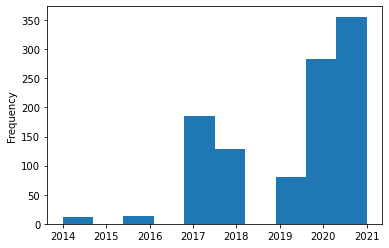
\includegraphics{assets/images/chapters/introduction-to-python/tutorial_74_1.png}

}

\caption{png}

\end{figure}

\hypertarget{filtering}{%
\section{6 - Filtering}\label{filtering}}

There are different ways of filtering data with Pandas:

\begin{itemize}
\tightlist
\item
  The \textbf{classic} method with bracket indexing/subsetting
\item
  The \texttt{query()} method
\end{itemize}

The classic method

\begin{Shaded}
\begin{Highlighting}[]
\CommentTok{\# Getting all the publications before 2015}
\NormalTok{sample\_df[sample\_df[}\StringTok{\textquotesingle{}publication\_year\textquotesingle{}}\NormalTok{]  }\OperatorTok{\textless{}} \DecValTok{2015}\NormalTok{ ]}
\end{Highlighting}
\end{Shaded}

project\_name

publication\_year

publication\_doi

site\_name

latitude

longitude

geo\_loc\_name

sample\_name

sample\_host

sample\_age

sample\_age\_doi

community\_type

material

archive

archive\_project

archive\_accession

0

Warinner2014

2014

10.1038/ng.2906

Dalheim

51.565

8.84

Germany

B61

Homo sapiens

900

10.1038/ng.2906

oral

dental calculus

SRA

PRJNA216965

SRS473742,SRS473743,SRS473744,SRS473745

1

Warinner2014

2014

10.1038/ng.2906

Dalheim

51.565

8.84

Germany

G12

Homo sapiens

900

10.1038/ng.2906

oral

dental calculus

SRA

PRJNA216965

SRS473747,SRS473746,SRS473748,SRS473749,SRS473750

272

Campana2014

2014

10.1186/1756-0500-7-111

Teposcolula Yucundaa

17.490

-97.46

Mexico

TP4

Homo sapiens

400

10.7183/1045-6635.23.4.467

skeletal tissue

bone

SRA

PRJNA205039

SRS428959

273

Campana2014

2014

10.1186/1756-0500-7-111

Teposcolula Yucundaa

17.490

-97.46

Mexico

TP10

Homo sapiens

400

10.7183/1045-6635.23.4.467

skeletal tissue

bone

SRA

PRJNA205039

SRS428961

274

Campana2014

2014

10.1186/1756-0500-7-111

Teposcolula Yucundaa

17.490

-97.46

Mexico

TP18

Homo sapiens

400

10.7183/1045-6635.23.4.467

skeletal tissue

bone

SRA

PRJNA205039

SRS428962

275

Campana2014

2014

10.1186/1756-0500-7-111

Teposcolula Yucundaa

17.490

-97.46

Mexico

TP37

Homo sapiens

400

10.7183/1045-6635.23.4.467

skeletal tissue

bone

SRA

PRJNA205039

SRS428963

276

Campana2014

2014

10.1186/1756-0500-7-111

Teposcolula Yucundaa

17.490

-97.46

Mexico

TP9

Homo sapiens

400

10.7183/1045-6635.23.4.467

skeletal tissue

bone

SRA

PRJNA205039

SRS428960

277

Campana2014

2014

10.1186/1756-0500-7-111

Teposcolula Yucundaa

17.490

-97.46

Mexico

TP48

Homo sapiens

400

10.7183/1045-6635.23.4.467

skeletal tissue

bone

SRA

PRJNA205039

SRS428964

278

Campana2014

2014

10.1186/1756-0500-7-111

Teposcolula Yucundaa

17.490

-97.46

Mexico

TP02,TP10,TP15,TP26

Homo sapiens

400

10.7183/1045-6635.23.4.467

skeletal tissue

bone

SRA

PRJNA205039

SRS428958

279

Campana2014

2014

10.1186/1756-0500-7-111

Teposcolula Yucundaa

17.490

-97.46

Mexico

TP32,TP42,TP45,TP48

Homo sapiens

400

10.7183/1045-6635.23.4.467

skeletal tissue

bone

SRA

PRJNA205039

SRS428972

500

Appelt2014

2014

10.1128/AEM.03242-13

Place d'Armes, Namur

50.460

4.86

Belgium

4.453

Homo sapiens

600

10.1128/AEM.03242-13

gut

palaeofaeces

SRA

PRJNA230469

SRS510175

\begin{Shaded}
\begin{Highlighting}[]
\CommentTok{\# Getting all the publications before 2015, only in the Northern hemisphere}
\NormalTok{sample\_df[(sample\_df[}\StringTok{\textquotesingle{}publication\_year\textquotesingle{}}\NormalTok{]  }\OperatorTok{\textless{}} \DecValTok{2015}\NormalTok{) }\OperatorTok{\&}\NormalTok{ (sample\_df[}\StringTok{\textquotesingle{}longitude\textquotesingle{}}\NormalTok{] }\OperatorTok{\textgreater{}} \DecValTok{0}\NormalTok{)]}
\end{Highlighting}
\end{Shaded}

project\_name

publication\_year

publication\_doi

site\_name

latitude

longitude

geo\_loc\_name

sample\_name

sample\_host

sample\_age

sample\_age\_doi

community\_type

material

archive

archive\_project

archive\_accession

0

Warinner2014

2014

10.1038/ng.2906

Dalheim

51.565

8.84

Germany

B61

Homo sapiens

900

10.1038/ng.2906

oral

dental calculus

SRA

PRJNA216965

SRS473742,SRS473743,SRS473744,SRS473745

1

Warinner2014

2014

10.1038/ng.2906

Dalheim

51.565

8.84

Germany

G12

Homo sapiens

900

10.1038/ng.2906

oral

dental calculus

SRA

PRJNA216965

SRS473747,SRS473746,SRS473748,SRS473749,SRS473750

500

Appelt2014

2014

10.1128/AEM.03242-13

Place d'Armes, Namur

50.460

4.86

Belgium

4.453

Homo sapiens

600

10.1128/AEM.03242-13

gut

palaeofaeces

SRA

PRJNA230469

SRS510175

This syntax can rapidly become quite cumbersome, which is why we can
also use the \texttt{query()} method

\begin{Shaded}
\begin{Highlighting}[]
\CommentTok{\# Getting all the publications before 2015}
\NormalTok{sample\_df.query(}\StringTok{"publication\_year \textless{} 2015"}\NormalTok{)}
\end{Highlighting}
\end{Shaded}

project\_name

publication\_year

publication\_doi

site\_name

latitude

longitude

geo\_loc\_name

sample\_name

sample\_host

sample\_age

sample\_age\_doi

community\_type

material

archive

archive\_project

archive\_accession

0

Warinner2014

2014

10.1038/ng.2906

Dalheim

51.565

8.84

Germany

B61

Homo sapiens

900

10.1038/ng.2906

oral

dental calculus

SRA

PRJNA216965

SRS473742,SRS473743,SRS473744,SRS473745

1

Warinner2014

2014

10.1038/ng.2906

Dalheim

51.565

8.84

Germany

G12

Homo sapiens

900

10.1038/ng.2906

oral

dental calculus

SRA

PRJNA216965

SRS473747,SRS473746,SRS473748,SRS473749,SRS473750

272

Campana2014

2014

10.1186/1756-0500-7-111

Teposcolula Yucundaa

17.490

-97.46

Mexico

TP4

Homo sapiens

400

10.7183/1045-6635.23.4.467

skeletal tissue

bone

SRA

PRJNA205039

SRS428959

273

Campana2014

2014

10.1186/1756-0500-7-111

Teposcolula Yucundaa

17.490

-97.46

Mexico

TP10

Homo sapiens

400

10.7183/1045-6635.23.4.467

skeletal tissue

bone

SRA

PRJNA205039

SRS428961

274

Campana2014

2014

10.1186/1756-0500-7-111

Teposcolula Yucundaa

17.490

-97.46

Mexico

TP18

Homo sapiens

400

10.7183/1045-6635.23.4.467

skeletal tissue

bone

SRA

PRJNA205039

SRS428962

275

Campana2014

2014

10.1186/1756-0500-7-111

Teposcolula Yucundaa

17.490

-97.46

Mexico

TP37

Homo sapiens

400

10.7183/1045-6635.23.4.467

skeletal tissue

bone

SRA

PRJNA205039

SRS428963

276

Campana2014

2014

10.1186/1756-0500-7-111

Teposcolula Yucundaa

17.490

-97.46

Mexico

TP9

Homo sapiens

400

10.7183/1045-6635.23.4.467

skeletal tissue

bone

SRA

PRJNA205039

SRS428960

277

Campana2014

2014

10.1186/1756-0500-7-111

Teposcolula Yucundaa

17.490

-97.46

Mexico

TP48

Homo sapiens

400

10.7183/1045-6635.23.4.467

skeletal tissue

bone

SRA

PRJNA205039

SRS428964

278

Campana2014

2014

10.1186/1756-0500-7-111

Teposcolula Yucundaa

17.490

-97.46

Mexico

TP02,TP10,TP15,TP26

Homo sapiens

400

10.7183/1045-6635.23.4.467

skeletal tissue

bone

SRA

PRJNA205039

SRS428958

279

Campana2014

2014

10.1186/1756-0500-7-111

Teposcolula Yucundaa

17.490

-97.46

Mexico

TP32,TP42,TP45,TP48

Homo sapiens

400

10.7183/1045-6635.23.4.467

skeletal tissue

bone

SRA

PRJNA205039

SRS428972

500

Appelt2014

2014

10.1128/AEM.03242-13

Place d'Armes, Namur

50.460

4.86

Belgium

4.453

Homo sapiens

600

10.1128/AEM.03242-13

gut

palaeofaeces

SRA

PRJNA230469

SRS510175

\begin{Shaded}
\begin{Highlighting}[]
\CommentTok{\# Getting all the publications before 2015, only the Northern hemisphere}
\NormalTok{sample\_df.query(}\StringTok{"publication\_year \textless{} 2015 and longitude \textgreater{} 0 "}\NormalTok{)}
\end{Highlighting}
\end{Shaded}

project\_name

publication\_year

publication\_doi

site\_name

latitude

longitude

geo\_loc\_name

sample\_name

sample\_host

sample\_age

sample\_age\_doi

community\_type

material

archive

archive\_project

archive\_accession

0

Warinner2014

2014

10.1038/ng.2906

Dalheim

51.565

8.84

Germany

B61

Homo sapiens

900

10.1038/ng.2906

oral

dental calculus

SRA

PRJNA216965

SRS473742,SRS473743,SRS473744,SRS473745

1

Warinner2014

2014

10.1038/ng.2906

Dalheim

51.565

8.84

Germany

G12

Homo sapiens

900

10.1038/ng.2906

oral

dental calculus

SRA

PRJNA216965

SRS473747,SRS473746,SRS473748,SRS473749,SRS473750

500

Appelt2014

2014

10.1128/AEM.03242-13

Place d'Armes, Namur

50.460

4.86

Belgium

4.453

Homo sapiens

600

10.1128/AEM.03242-13

gut

palaeofaeces

SRA

PRJNA230469

SRS510175

\hypertarget{groupby-operations-and-computing-statistics-on-grouped-values}{%
\section{7 - GroupBy operations, and computing statistics on grouped
values}\label{groupby-operations-and-computing-statistics-on-grouped-values}}

The ``groupBy'' operation, as the name suggests, allows us to group
values by a grouping key, and perform a groupwise operation.\\
For example, we can group by the \texttt{sample\_host} and get the age
of the \textbf{youngest} sample in each group

\begin{Shaded}
\begin{Highlighting}[]
\NormalTok{sample\_df.groupby(}\StringTok{"sample\_host"}\NormalTok{)[}\StringTok{\textquotesingle{}sample\_age\textquotesingle{}}\NormalTok{].}\BuiltInTok{min}\NormalTok{()}
\end{Highlighting}
\end{Shaded}

\begin{verbatim}
sample_host
Alouatta palliata                   200
Ambrosia artemisiifolia             100
Arabidopsis thaliana                100
Canis lupus                         400
Conepatus chinga                    100
Gerbilliscus boehmi                 100
Gorilla beringei                    100
Gorilla beringei beringei           200
Gorilla beringei graueri            200
Gorilla gorilla gorilla             200
Homo sapiens                        100
Homo sapiens neanderthalensis     35800
Mammuthus primigenius             41800
Pan troglodytes                     100
Pan troglodytes ellioti             200
Pan troglodytes schweinfurthii      100
Pan troglodytes verus               200
Papio anubis                        100
Papio hamadryas                     100
Papio sp.                           100
Rangifer tarandus                   100
Strigocuscus celebensis             100
Ursus arctos                        100
Name: sample_age, dtype: int64
\end{verbatim}

Here \texttt{min()} is a so-called aggregation function

Notice that \texttt{.value\_counts()} is actually a special case of
\texttt{.groupby()}

\begin{Shaded}
\begin{Highlighting}[]
\NormalTok{sample\_df.groupby(}\StringTok{"sample\_host"}\NormalTok{)[}\StringTok{"sample\_host"}\NormalTok{].count()}
\end{Highlighting}
\end{Shaded}

\begin{verbatim}
sample_host
Alouatta palliata                   5
Ambrosia artemisiifolia            46
Arabidopsis thaliana               34
Canis lupus                        12
Conepatus chinga                    4
Gerbilliscus boehmi                 4
Gorilla beringei                    2
Gorilla beringei beringei          15
Gorilla beringei graueri            6
Gorilla gorilla gorilla             8
Homo sapiens                      741
Homo sapiens neanderthalensis      32
Mammuthus primigenius               8
Pan troglodytes                     1
Pan troglodytes ellioti             6
Pan troglodytes schweinfurthii     26
Pan troglodytes verus               7
Papio anubis                        2
Papio hamadryas                     5
Papio sp.                           1
Rangifer tarandus                   6
Strigocuscus celebensis             4
Ursus arctos                       85
Name: sample_host, dtype: int64
\end{verbatim}

\hypertarget{reshaping-data-from-wide-to-long-and-back}{%
\section{8 - Reshaping data, from wide to long and
back}\label{reshaping-data-from-wide-to-long-and-back}}

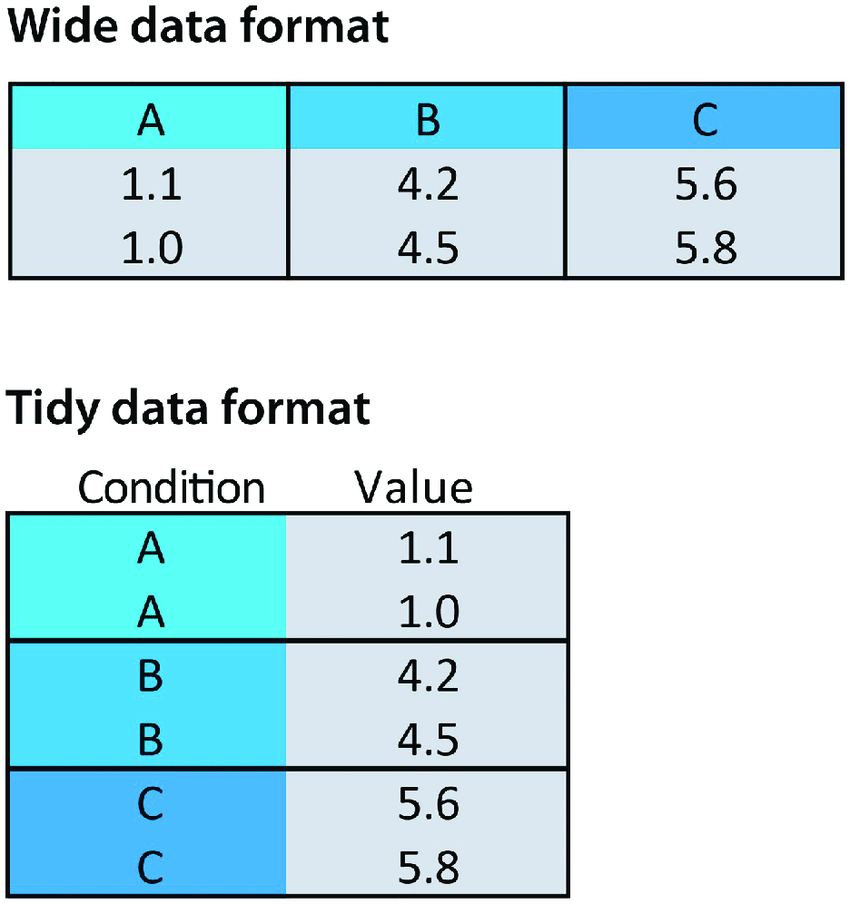
\includegraphics{assets/images/chapters/introduction-to-python/The-wide-versus-tidy-data-format-In-the-wide-spreadsheet-like-data-format-each-column.png}

\hypertarget{from-wide-to-longtidy}{%
\subsection{From wide to long/tidy}\label{from-wide-to-longtidy}}

The tidy format, or long format idea is that one column = one kind of
data.\\
Unfortunately for this tutorial, the AncientMetagenomeDir tables are
already in the tidy format (good), so we'll see an example or the wide
format just below

\begin{Shaded}
\begin{Highlighting}[]
\NormalTok{wide\_df }\OperatorTok{=}\NormalTok{ pd.DataFrame(}
\NormalTok{    [}
\NormalTok{    [}\DecValTok{150}\NormalTok{,}\DecValTok{155}\NormalTok{,}\DecValTok{157}\NormalTok{,}\DecValTok{160}\NormalTok{],}
\NormalTok{    [}\DecValTok{149}\NormalTok{,}\DecValTok{153}\NormalTok{,}\DecValTok{154}\NormalTok{,}\DecValTok{155}\NormalTok{]}
\NormalTok{    ]}
\NormalTok{    , index }\OperatorTok{=}\NormalTok{ [}\StringTok{\textquotesingle{}John\textquotesingle{}}\NormalTok{,}\StringTok{\textquotesingle{}Jack\textquotesingle{}}\NormalTok{]}
\NormalTok{    , columns }\OperatorTok{=}\NormalTok{ [}\DecValTok{1991}\NormalTok{,}\DecValTok{1992}\NormalTok{,}\DecValTok{1993}\NormalTok{, }\DecValTok{1994}\NormalTok{]}
\NormalTok{).rename\_axis(}\StringTok{\textquotesingle{}individual\textquotesingle{}}\NormalTok{).reset\_index()}
\NormalTok{wide\_df}
\end{Highlighting}
\end{Shaded}

individual

1991

1992

1993

1994

0

John

150

155

157

160

1

Jack

149

153

154

155

In this hypothetic dataframe, we have the years as column, the
individual as index, and their height as value.\\
We'll reformat to the tidy/long format using the \texttt{.melt()}
function

\begin{Shaded}
\begin{Highlighting}[]
\NormalTok{tidy\_df }\OperatorTok{=}\NormalTok{ wide\_df.melt(id\_vars}\OperatorTok{=}\StringTok{\textquotesingle{}individual\textquotesingle{}}\NormalTok{, var\_name}\OperatorTok{=}\StringTok{\textquotesingle{}birthyear\textquotesingle{}}\NormalTok{, value\_name}\OperatorTok{=}\StringTok{\textquotesingle{}height\textquotesingle{}}\NormalTok{)}
\NormalTok{tidy\_df}
\end{Highlighting}
\end{Shaded}

individual

birthyear

height

0

John

1991

150

1

Jack

1991

149

2

John

1992

155

3

Jack

1992

153

4

John

1993

157

5

Jack

1993

154

6

John

1994

160

7

Jack

1994

155

\begin{quote}
Bonus: How to deal with a dataframe with the kind of data indicated in
the column name, typically like so
\end{quote}

\begin{Shaded}
\begin{Highlighting}[]
\NormalTok{wide\_df }\OperatorTok{=}\NormalTok{ pd.DataFrame(}
\NormalTok{    [}
\NormalTok{    [}\DecValTok{150}\NormalTok{,}\DecValTok{155}\NormalTok{,}\DecValTok{157}\NormalTok{,}\DecValTok{160}\NormalTok{],}
\NormalTok{    [}\DecValTok{149}\NormalTok{,}\DecValTok{153}\NormalTok{,}\DecValTok{154}\NormalTok{,}\DecValTok{155}\NormalTok{]}
\NormalTok{    ]}
\NormalTok{    , index }\OperatorTok{=}\NormalTok{ [}\StringTok{\textquotesingle{}John\textquotesingle{}}\NormalTok{,}\StringTok{\textquotesingle{}Jack\textquotesingle{}}\NormalTok{]}
\NormalTok{    , columns }\OperatorTok{=}\NormalTok{ [}\StringTok{"year{-}1991"}\NormalTok{,}\StringTok{"year{-}1992"}\NormalTok{,}\StringTok{"year{-}1993"}\NormalTok{, }\StringTok{"year{-}1994"}\NormalTok{]}
\NormalTok{).rename\_axis(}\StringTok{\textquotesingle{}individual\textquotesingle{}}\NormalTok{).reset\_index()}
\NormalTok{wide\_df}
\end{Highlighting}
\end{Shaded}

individual

year-1991

year-1992

year-1993

year-1994

0

John

150

155

157

160

1

Jack

149

153

154

155

\begin{Shaded}
\begin{Highlighting}[]
\NormalTok{pd.wide\_to\_long(wide\_df, [}\StringTok{\textquotesingle{}year\textquotesingle{}}\NormalTok{], i}\OperatorTok{=}\StringTok{\textquotesingle{}individual\textquotesingle{}}\NormalTok{, j}\OperatorTok{=}\StringTok{\textquotesingle{}birthyear\textquotesingle{}}\NormalTok{, sep}\OperatorTok{=}\StringTok{"{-}"}\NormalTok{).rename(columns}\OperatorTok{=}\NormalTok{\{}\StringTok{\textquotesingle{}year\textquotesingle{}}\NormalTok{:}\StringTok{\textquotesingle{}height\textquotesingle{}}\NormalTok{\})}
\end{Highlighting}
\end{Shaded}

height

individual

birthyear

John

1991

150

Jack

1991

149

John

1992

155

Jack

1992

153

John

1993

157

Jack

1993

154

John

1994

160

Jack

1994

155

\hypertarget{from-longtidy-to-wide-format-using-the-.pivot-function.}{%
\subsection{\texorpdfstring{From long/tidy to wide format using the
\texttt{.pivot()}
function.}{From long/tidy to wide format using the .pivot() function.}}\label{from-longtidy-to-wide-format-using-the-.pivot-function.}}

\begin{Shaded}
\begin{Highlighting}[]
\NormalTok{tidy\_df.pivot(index}\OperatorTok{=}\StringTok{\textquotesingle{}individual\textquotesingle{}}\NormalTok{, columns}\OperatorTok{=}\StringTok{\textquotesingle{}birthyear\textquotesingle{}}\NormalTok{, values}\OperatorTok{=}\StringTok{\textquotesingle{}height\textquotesingle{}}\NormalTok{)}
\end{Highlighting}
\end{Shaded}

\begin{verbatim}
/Users/maxime/mambaforge/envs/intro-data/lib/python3.10/site-packages/pandas/core/algorithms.py:798: FutureWarning: In a future version, the Index constructor will not infer numeric dtypes when passed object-dtype sequences (matching Series behavior)
\end{verbatim}

birthyear

1991

1992

1993

1994

individual

Jack

149

153

154

155

John

150

155

157

160

\hypertarget{joining-two-different-tables}{%
\section{9 - Joining two different
tables}\label{joining-two-different-tables}}

In AncientMetagenomeDir, the information about each sample is located in
sample table, and about the library in the library table.\\
To match these two together, we need to join the tables together.

To do so, we need a column in common between the two tables, the
so-called \textbf{joining key} (this key can be the index)

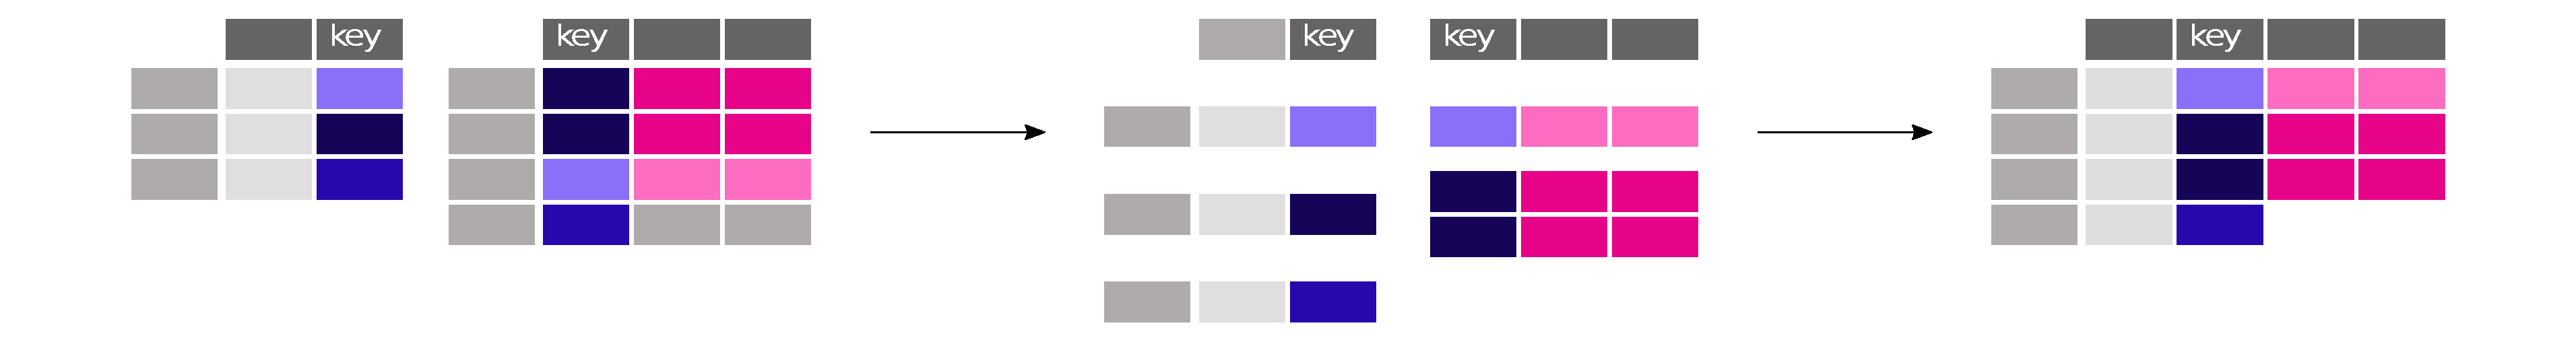
\includegraphics{index_files/mediabag/assets/images/chapters/introduction-to-python/08_merge_left.pdf}

For the samples and libraries dataframe, the joining key is the column
\texttt{sample\_name}

\begin{Shaded}
\begin{Highlighting}[]
\NormalTok{sample\_df.merge(library\_df, on}\OperatorTok{=}\StringTok{\textquotesingle{}sample\_name\textquotesingle{}}\NormalTok{).columns}
\end{Highlighting}
\end{Shaded}

\begin{verbatim}
Index(['project_name_x', 'publication_year_x', 'publication_doi', 'site_name',
       'latitude', 'longitude', 'geo_loc_name', 'sample_name', 'sample_host',
       'sample_age', 'sample_age_doi', 'community_type', 'material',
       'archive_x', 'archive_project_x', 'archive_accession', 'project_name_y',
       'publication_year_y', 'data_publication_doi', 'archive_y',
       'archive_project_y', 'archive_sample_accession', 'library_name',
       'strand_type', 'library_polymerase', 'library_treatment',
       'library_concentration', 'instrument_model', 'library_layout',
       'library_strategy', 'read_count', 'archive_data_accession',
       'download_links', 'download_md5s', 'download_sizes'],
      dtype='object')
\end{verbatim}

We have some duplicate columns that we can get rid of:

\begin{Shaded}
\begin{Highlighting}[]
\NormalTok{merged\_df }\OperatorTok{=}\NormalTok{ sample\_df.merge(library\_df.drop([}\StringTok{\textquotesingle{}project\_name\textquotesingle{}}\NormalTok{, }\StringTok{\textquotesingle{}publication\_year\textquotesingle{}}\NormalTok{, }\StringTok{\textquotesingle{}archive\_project\textquotesingle{}}\NormalTok{, }\StringTok{\textquotesingle{}archive\textquotesingle{}}\NormalTok{], axis}\OperatorTok{=}\DecValTok{1}\NormalTok{), on}\OperatorTok{=}\StringTok{\textquotesingle{}sample\_name\textquotesingle{}}\NormalTok{)}
\NormalTok{merged\_df}
\end{Highlighting}
\end{Shaded}

project\_name

publication\_year

publication\_doi

site\_name

latitude

longitude

geo\_loc\_name

sample\_name

sample\_host

sample\_age

\ldots{}

library\_treatment

library\_concentration

instrument\_model

library\_layout

library\_strategy

read\_count

archive\_data\_accession

download\_links

download\_md5s

download\_sizes

0

Warinner2014

2014

10.1038/ng.2906

Dalheim

51.565

8.84

Germany

B61

Homo sapiens

900

\ldots{}

none

NaN

Illumina HiSeq 2000

SINGLE

WGS

13228381

SRR957738

ftp.sra.ebi.ac.uk/vol1/fastq/SRR957/SRR957738/\ldots{}

9c40c43b5d455e760ae8db924347f0b2

953396663

1

Warinner2014

2014

10.1038/ng.2906

Dalheim

51.565

8.84

Germany

B61

Homo sapiens

900

\ldots{}

none

NaN

Illumina HiSeq 2000

SINGLE

WGS

13260566

SRR957739

ftp.sra.ebi.ac.uk/vol1/fastq/SRR957/SRR957739/\ldots{}

dec1507f742de109529638bf00e0732f

1026825795

2

Warinner2014

2014

10.1038/ng.2906

Dalheim

51.565

8.84

Germany

B61

Homo sapiens

900

\ldots{}

none

NaN

Illumina HiSeq 2000

SINGLE

WGS

8869866

SRR957740

ftp.sra.ebi.ac.uk/vol1/fastq/SRR957/SRR957740/\ldots{}

bc49c59f489b4009206f8abcb737d55d

661500786

3

Warinner2014

2014

10.1038/ng.2906

Dalheim

51.565

8.84

Germany

B61

Homo sapiens

900

\ldots{}

none

NaN

Illumina HiSeq 2000

SINGLE

WGS

11275013

SRR957741

ftp.sra.ebi.ac.uk/vol1/fastq/SRR957/SRR957741/\ldots{}

e02e3549ddd3ba6dc278a7f573c07321

877360302

4

Warinner2014

2014

10.1038/ng.2906

Dalheim

51.565

8.84

Germany

G12

Homo sapiens

900

\ldots{}

none

NaN

Illumina HiSeq 2000

SINGLE

WGS

8978974

SRR957742

ftp.sra.ebi.ac.uk/vol1/fastq/SRR957/SRR957742/\ldots{}

b7c620b8ee165c08bee204529341ca5b

690614774

\ldots{}

\ldots{}

\ldots{}

\ldots{}

\ldots{}

\ldots{}

\ldots{}

\ldots{}

\ldots{}

\ldots{}

\ldots{}

\ldots{}

\ldots{}

\ldots{}

\ldots{}

\ldots{}

\ldots{}

\ldots{}

\ldots{}

\ldots{}

\ldots{}

\ldots{}

1802

Maixner2021

2021

10.1016/j.cub.2021.09.031

Edlersbergwerk - oben, Hallstatt

47.560

13.63

Austria

2612

Homo sapiens

150

\ldots{}

none

NaN

Illumina MiSeq

PAIRED

WGS

1858404

ERR5766179

ftp.sra.ebi.ac.uk/vol1/fastq/ERR576/009/ERR576\ldots{}

542787c645b0aeebe15c66cc926d3f69;0bc58d56be3c3\ldots{}

86783041;98100690

1803

Maixner2021

2021

10.1016/j.cub.2021.09.031

Edlersbergwerk - oben, Hallstatt

47.560

13.63

Austria

2612

Homo sapiens

150

\ldots{}

none

NaN

Illumina MiSeq

PAIRED

WGS

1603064

ERR5766180

ftp.sra.ebi.ac.uk/vol1/fastq/ERR576/000/ERR576\ldots{}

022bb28da460e66590e974b4135bdd2e;f88acec67b648\ldots{}

74375931;77621627

1804

Maixner2021

2021

10.1016/j.cub.2021.09.031

Edlersbergwerk - oben, Hallstatt

47.560

13.63

Austria

2612

Homo sapiens

150

\ldots{}

none

NaN

Illumina MiSeq

PAIRED

WGS

1075088

ERR5766181

ftp.sra.ebi.ac.uk/vol1/fastq/ERR576/001/ERR576\ldots{}

57fc575d32db14f1d5c1ed7f6a106e91;4f57b9d978b53\ldots{}

51852071;56288763

1805

Maixner2021

2021

10.1016/j.cub.2021.09.031

Edlersbergwerk - oben, Hallstatt

47.560

13.63

Austria

2612

Homo sapiens

150

\ldots{}

none

NaN

Illumina HiSeq 2500

PAIRED

WGS

138836358

ERR5766182

ftp.sra.ebi.ac.uk/vol1/fastq/ERR576/002/ERR576\ldots{}

64e63df8da7542957d1d9eb08e764d38;3fc6cba02c74d\ldots{}

4332353625;4420486328

1806

Maixner2021

2021

10.1016/j.cub.2021.09.031

Edlersbergwerk - oben, Hallstatt

47.560

13.63

Austria

2612

Homo sapiens

150

\ldots{}

none

NaN

HiSeq X Ten

PAIRED

WGS

84192332

ERR5766183

ftp.sra.ebi.ac.uk/vol1/fastq/ERR576/003/ERR576\ldots{}

43ac661c4e211ed6ee2940dcab8b13cb;88de66a85df92\ldots{}

3128863954;3460789287

1807 rows × 31 columns

\hypertarget{visualizing-some-of-the-results-with-plotnine}{%
\section{10 - Visualizing some of the results with
Plotnine}\label{visualizing-some-of-the-results-with-plotnine}}

Plotnine is the Python clone of ggplot2, the syntax is identical, which
makes it great if you're working with data in tidy/long format, and are
already familiar with the ggplot2 syntax

\begin{Shaded}
\begin{Highlighting}[]
\NormalTok{ggplot(merged\_df, aes(x}\OperatorTok{=}\StringTok{\textquotesingle{}publication\_year\textquotesingle{}}\NormalTok{)) }\OperatorTok{+}\NormalTok{ geom\_histogram() }\OperatorTok{+}\NormalTok{ theme\_classic()}
\end{Highlighting}
\end{Shaded}

\begin{verbatim}
/Users/maxime/mambaforge/envs/intro-data/lib/python3.10/
site-packages/plotnine/stats/stat_bin.py:95:
PlotnineWarning: 'stat_bin()' using 'bins = 15'. Pick better value with 'binwidth'.
\end{verbatim}

\begin{figure}

{\centering 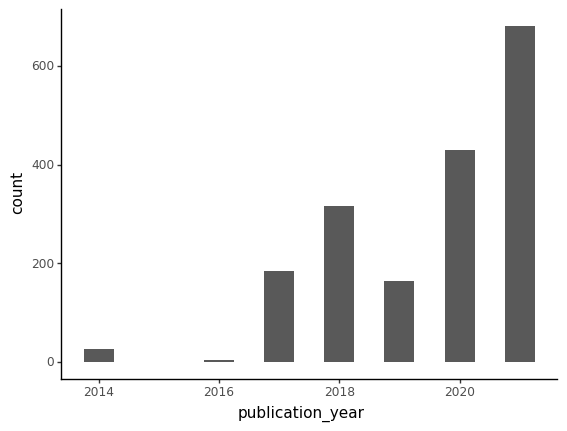
\includegraphics{assets/images/chapters/introduction-to-python/tutorial_111_1.png}

}

\caption{png}

\end{figure}

\begin{verbatim}
<ggplot: (366051178)>
\end{verbatim}

We can start to ask some questions, for example, is the sequencing depth
increasing with the years ?

\begin{Shaded}
\begin{Highlighting}[]
\NormalTok{merged\_df[}\StringTok{\textquotesingle{}publication\_year\textquotesingle{}}\NormalTok{] }\OperatorTok{=}\NormalTok{ merged\_df[}\StringTok{\textquotesingle{}publication\_year\textquotesingle{}}\NormalTok{].astype(}\StringTok{\textquotesingle{}category\textquotesingle{}}\NormalTok{)}
\end{Highlighting}
\end{Shaded}

\begin{Shaded}
\begin{Highlighting}[]
\NormalTok{ggplot(merged\_df, aes(x}\OperatorTok{=}\StringTok{\textquotesingle{}publication\_year\textquotesingle{}}\NormalTok{, y}\OperatorTok{=}\StringTok{\textquotesingle{}np.log10(read\_count)\textquotesingle{}}\NormalTok{, fill}\OperatorTok{=}\StringTok{\textquotesingle{}publication\_year\textquotesingle{}}\NormalTok{)) }\OperatorTok{+}
\NormalTok{geom\_jitter(alpha}\OperatorTok{=}\FloatTok{0.1}\NormalTok{) }\OperatorTok{+}\NormalTok{ geom\_boxplot(alpha}\OperatorTok{=}\FloatTok{0.8}\NormalTok{) }\OperatorTok{+}\NormalTok{ theme\_classic()}
\end{Highlighting}
\end{Shaded}

\begin{figure}

{\centering 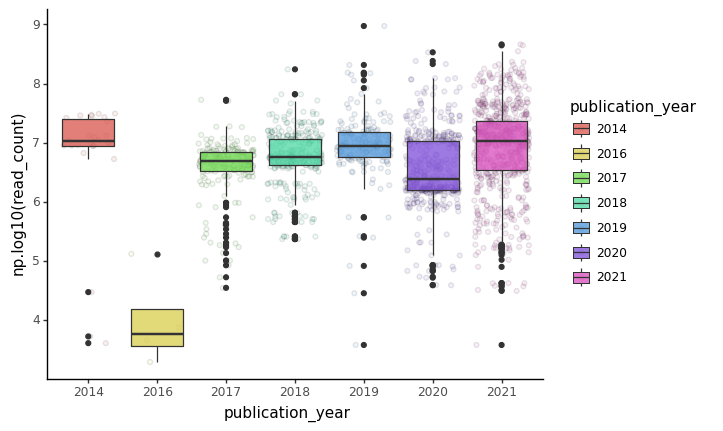
\includegraphics{assets/images/chapters/introduction-to-python/tutorial_114_0.png}

}

\caption{png}

\end{figure}

\begin{verbatim}
<ggplot: (366112582)>
\end{verbatim}

We could ask the same question, but first grouping the samples by
publication year

\begin{Shaded}
\begin{Highlighting}[]
\NormalTok{avg\_read\_count\_by\_year }\OperatorTok{=}\NormalTok{ merged\_df.groupby(}\StringTok{\textquotesingle{}publication\_year\textquotesingle{}}\NormalTok{)[}\StringTok{\textquotesingle{}read\_count\textquotesingle{}}\NormalTok{].mean().to\_frame().reset\_index()}
\NormalTok{avg\_read\_count\_by\_year}
\end{Highlighting}
\end{Shaded}

publication\_year

read\_count

0

2014

1.437173e+07

1

2016

3.653450e+04

2

2017

5.712598e+06

3

2018

9.273287e+06

4

2019

2.211632e+07

5

2020

1.111819e+07

6

2021

2.547655e+07

\begin{Shaded}
\begin{Highlighting}[]
\NormalTok{ggplot(avg\_read\_count\_by\_year, aes(x}\OperatorTok{=}\StringTok{\textquotesingle{}publication\_year\textquotesingle{}}\NormalTok{, y}\OperatorTok{=}\StringTok{\textquotesingle{}np.log10(read\_count)\textquotesingle{}}\NormalTok{, fill}\OperatorTok{=}\StringTok{\textquotesingle{}publication\_year\textquotesingle{}}\NormalTok{)) }\OperatorTok{+}\NormalTok{ geom\_point()}
\end{Highlighting}
\end{Shaded}

\begin{figure}

{\centering 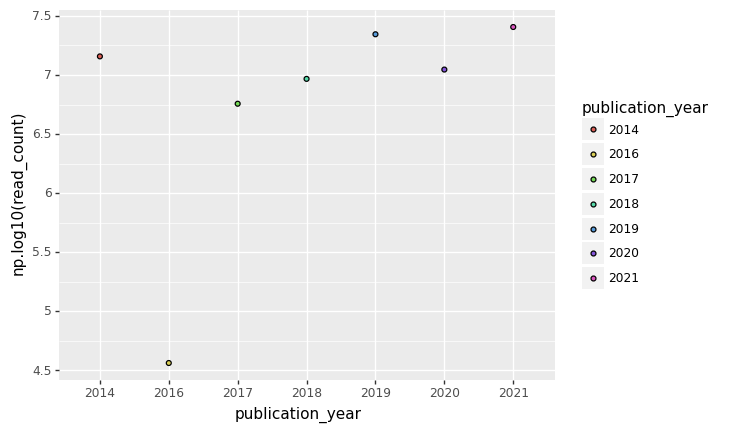
\includegraphics{assets/images/chapters/introduction-to-python/tutorial_117_0.png}

}

\caption{png}

\end{figure}

\begin{verbatim}
<ggplot: (366206706)>
\end{verbatim}

\textbf{Your turn ! Make a plot to investigate the relation between the
type of library treatment throughout the publication years}

\hypertarget{bonus-dealing-with-ill-formatted-columns}{%
\section{11 - Bonus, dealing with ill-formatted
columns}\label{bonus-dealing-with-ill-formatted-columns}}

Sometimes, colums can contains entries which could be split in multiple
columns, typically values separated by a comma. In AncientMetagenomeDir,
this is the case with the archive accession column.

Here is how we would solve it with pandas

\begin{Shaded}
\begin{Highlighting}[]
\NormalTok{sample\_df.assign(archive\_accession }\OperatorTok{=}\NormalTok{ sample\_df.archive\_accession.}\BuiltInTok{str}\NormalTok{.split(}\StringTok{","}\NormalTok{)).explode(}\StringTok{\textquotesingle{}archive\_accession\textquotesingle{}}\NormalTok{)}
\end{Highlighting}
\end{Shaded}

project\_name

publication\_year

publication\_doi

site\_name

latitude

longitude

geo\_loc\_name

sample\_name

sample\_host

sample\_age

sample\_age\_doi

community\_type

material

archive

archive\_project

archive\_accession

0

Warinner2014

2014

10.1038/ng.2906

Dalheim

51.565

8.840

Germany

B61

Homo sapiens

900

10.1038/ng.2906

oral

dental calculus

SRA

PRJNA216965

SRS473742

0

Warinner2014

2014

10.1038/ng.2906

Dalheim

51.565

8.840

Germany

B61

Homo sapiens

900

10.1038/ng.2906

oral

dental calculus

SRA

PRJNA216965

SRS473743

0

Warinner2014

2014

10.1038/ng.2906

Dalheim

51.565

8.840

Germany

B61

Homo sapiens

900

10.1038/ng.2906

oral

dental calculus

SRA

PRJNA216965

SRS473744

0

Warinner2014

2014

10.1038/ng.2906

Dalheim

51.565

8.840

Germany

B61

Homo sapiens

900

10.1038/ng.2906

oral

dental calculus

SRA

PRJNA216965

SRS473745

1

Warinner2014

2014

10.1038/ng.2906

Dalheim

51.565

8.840

Germany

G12

Homo sapiens

900

10.1038/ng.2906

oral

dental calculus

SRA

PRJNA216965

SRS473747

\ldots{}

\ldots{}

\ldots{}

\ldots{}

\ldots{}

\ldots{}

\ldots{}

\ldots{}

\ldots{}

\ldots{}

\ldots{}

\ldots{}

\ldots{}

\ldots{}

\ldots{}

\ldots{}

\ldots{}

1057

Kazarina2021b

2021

10.1016/j.jasrep.2021.103213

St.~Gertrude's Church, Riga

56.958

24.121

Latvia

T9

Homo sapiens

400

10.1016/j.jasrep.2021.103213

oral

tooth

ENA

PRJEB47251

ERS7283099

1058

Kazarina2021b

2021

10.1016/j.jasrep.2021.103213

Dom Square, Riga

56.949

24.104

Latvia

TZA3

Homo sapiens

400

10.1016/j.jasrep.2021.103213

oral

tooth

ENA

PRJEB47251

ERS7283100

1058

Kazarina2021b

2021

10.1016/j.jasrep.2021.103213

Dom Square, Riga

56.949

24.104

Latvia

TZA3

Homo sapiens

400

10.1016/j.jasrep.2021.103213

oral

tooth

ENA

PRJEB47251

ERS7283101

1059

Kazarina2021b

2021

10.1016/j.jasrep.2021.103213

St.~Peter's Church, Riga

56.947

24.109

Latvia

TZA4

Homo sapiens

500

10.1016/j.jasrep.2021.103213

oral

tooth

ENA

PRJEB47251

ERS7283102

1059

Kazarina2021b

2021

10.1016/j.jasrep.2021.103213

St.~Peter's Church, Riga

56.947

24.109

Latvia

TZA4

Homo sapiens

500

10.1016/j.jasrep.2021.103213

oral

tooth

ENA

PRJEB47251

ERS7283103

1262 rows × 16 columns

\hypertarget{introduction-to-github}{%
\chapter{Introduction to Git(Hub)}\label{introduction-to-github}}

\hypertarget{introduction-2}{%
\section{Introduction}\label{introduction-2}}

In this walkthrough, we will introduce the version control system
\textbf{Git} as well as \textbf{Github}, a remote hosting service for
version controlled repositories. Git and Github are increasingly popular
tools for tracking data, collaborating on research projects, and sharing
data and code, and learning to use them will help in many aspects of
your own research. For more information on the benefits of using version
control systems, see the slides.

\begin{tcolorbox}[enhanced jigsaw, opacitybacktitle=0.6, bottomtitle=1mm, opacityback=0, colback=white, coltitle=black, leftrule=.75mm, toprule=.15mm, title=\textcolor{quarto-callout-tip-color}{\faLightbulb}\hspace{0.5em}{Tip}, colframe=quarto-callout-tip-color-frame, toptitle=1mm, arc=.35mm, left=2mm, titlerule=0mm, breakable, rightrule=.15mm, bottomrule=.15mm, colbacktitle=quarto-callout-tip-color!10!white]

For this chapter's exercises, if not already performed, you will need to
create the \protect\hyperlink{creating-a-conda-environment}{conda
environment} from the \texttt{yml} file in the following
\href{https://doi.org/10.5281/zenodo.6983119}{archive}, and activate the
environment:

\begin{Shaded}
\begin{Highlighting}[]
\ExtensionTok{conda}\NormalTok{ activate git{-}eager}
\end{Highlighting}
\end{Shaded}

\end{tcolorbox}

\hypertarget{lecture-8}{%
\section{Lecture}\label{lecture-8}}

PDF version of these slides can be downloaded from
\href{https://github.com/SPAAM-community/https://github.com/SPAAM-community/wss-summer-school/raw/main/docs/raw/main/docs/assets/slides/2022/2b-intro-to-github/SPAAM\%20Summer\%20School\%202022\%20-\%202B\%20-\%20Introduction\%20to\%20Git(Hub).pdf}{here}.

\hypertarget{ssh-setup}{%
\section{SSH setup}\label{ssh-setup}}

To begin, you will set up an SSH key to facilitate easier authentication
when transferring data between local and remote repositories. In other
words, follow this section of the tutorial so that you never have to
type in your github password again! Begin by activating the conda
environment for this section (see \textbf{Preparation} above).

\begin{Shaded}
\begin{Highlighting}[]
\ExtensionTok{conda}\NormalTok{ activate git{-}eager}
\end{Highlighting}
\end{Shaded}

Next, generate your own ssh key, replacing the email below with your own
address.

\begin{Shaded}
\begin{Highlighting}[]
\FunctionTok{ssh{-}keygen} \AttributeTok{{-}t}\NormalTok{ ed25519 }\AttributeTok{{-}C} \StringTok{"your\_email@example.com"}
\end{Highlighting}
\end{Shaded}

I recommend saving the file to the default location and skipping
passphrase setup. To do this, simply press enter without typing
anything.

You should now (hopefully!) have generated an ssh key. To check that it
worked, run the following commands to list the files containing your
public and private keys and check that the ssh program is running.

\begin{Shaded}
\begin{Highlighting}[]
\BuiltInTok{cd}\NormalTok{ \textasciitilde{}/.ssh/}
\FunctionTok{ls}\NormalTok{ id}\PreprocessorTok{*}
\BuiltInTok{eval} \StringTok{"}\VariableTok{$(}\FunctionTok{ssh{-}agent} \AttributeTok{{-}s}\VariableTok{)}\StringTok{"}
\end{Highlighting}
\end{Shaded}

Now you need to give ssh your key to record:

\begin{Shaded}
\begin{Highlighting}[]
\FunctionTok{ssh{-}add}\NormalTok{ \textasciitilde{}/.ssh/id\_ed15519}
\end{Highlighting}
\end{Shaded}

Next, open your webbrowser and navigate to your github account. Go to
settings -\textgreater{} SSH \& GPG Keys -\textgreater{} New SSH Key.
Give you key a title and paste the public key that you just generated on
your local machine.

\begin{Shaded}
\begin{Highlighting}[]
\FunctionTok{cat}\NormalTok{ \textasciitilde{}/.ssh/id\_ed15519}
\end{Highlighting}
\end{Shaded}

Finally, press Add SSH key. To check that it worked, run the following
command on your local machine. You should see a message telling you that
you've successfully authenticated.

\begin{Shaded}
\begin{Highlighting}[]
\FunctionTok{ssh} \AttributeTok{{-}T}\NormalTok{ git@github.com}
\end{Highlighting}
\end{Shaded}

For more information about setting up the SSH key, including
instructions for different operating systems, check out github's
documentation:
\url{https://docs.github.com/es/authentication/connecting-to-github-with-ssh/generating-a-new-ssh-key-and-adding-it-to-the-ssh-agent}.

\hypertarget{the-only-6-commands-you-really-need-to-know}{%
\section{The only 6 commands you really need to
know}\label{the-only-6-commands-you-really-need-to-know}}

Now that you have set up your own SSH key, we can begin working on some
version controlled data! Navigate to your github homepage and create a
new repository. You can choose any name for your new repo (including the
default). Add a README file, then select Create Repository.

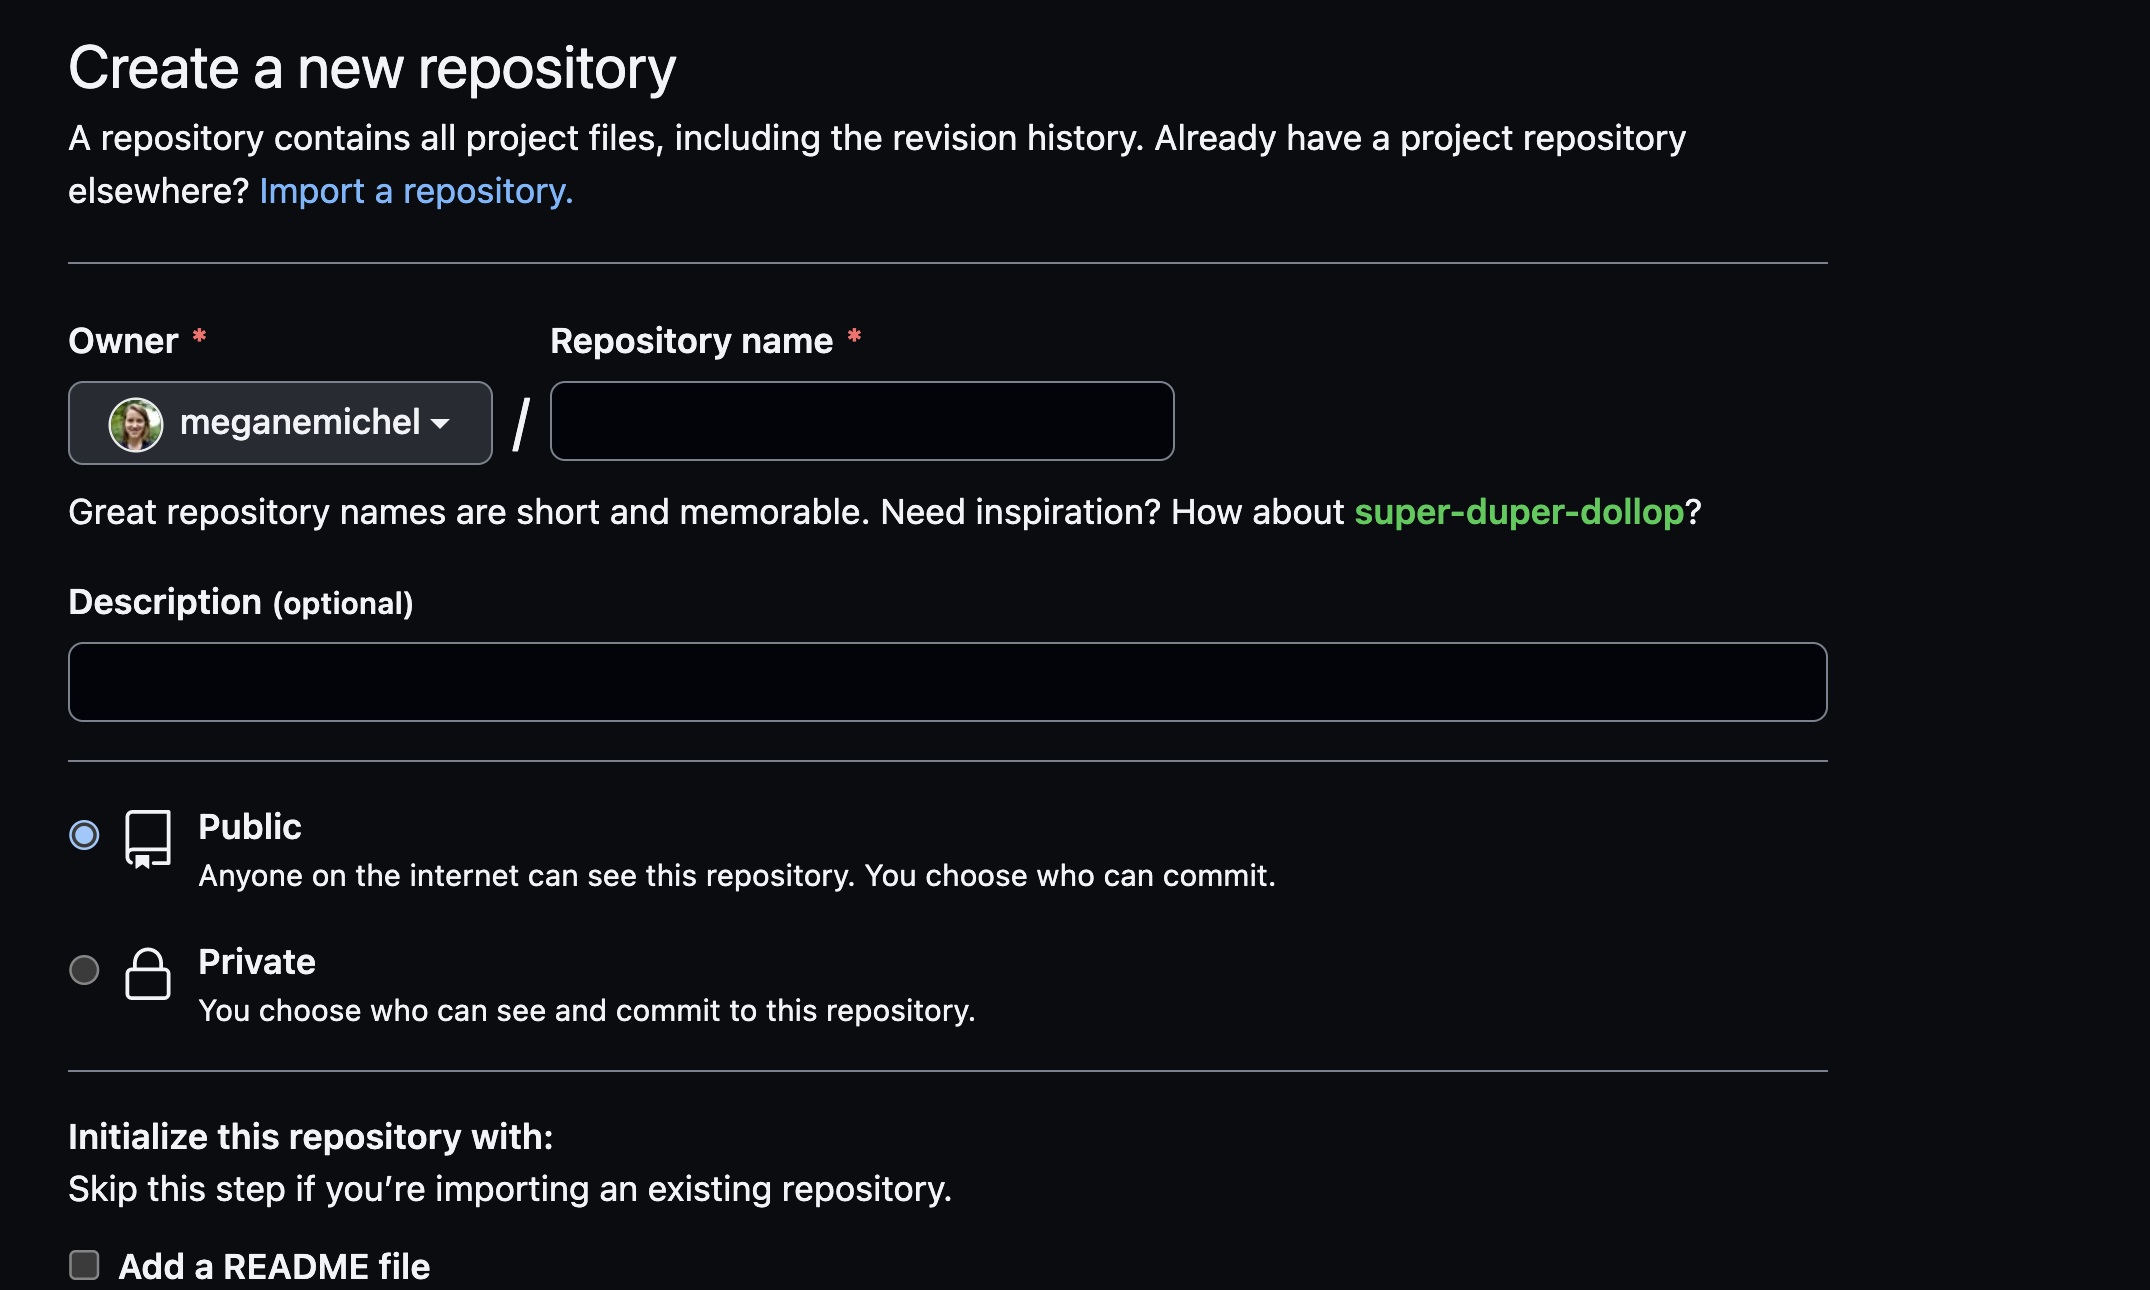
\includegraphics{assets/images/chapters/introduction-to-git/create_repo.png}

\begin{tcolorbox}[enhanced jigsaw, opacitybacktitle=0.6, bottomtitle=1mm, opacityback=0, colback=white, coltitle=black, leftrule=.75mm, toprule=.15mm, title=\textcolor{quarto-callout-note-color}{\faInfo}\hspace{0.5em}{Note}, colframe=quarto-callout-note-color-frame, toptitle=1mm, arc=.35mm, left=2mm, titlerule=0mm, breakable, rightrule=.15mm, bottomrule=.15mm, colbacktitle=quarto-callout-note-color!10!white]

For the remainder of the session, replace the name of my repository
(vigilant-octo-journey) with your own repo name.

\end{tcolorbox}

Change into the directory where you would like to work, and let's get
started! First, we will learn to \textbf{clone} a remote repository onto
your local machine. Navigate to your new repo, select the \emph{Code}
dropdown menu, select SSH, and copy the address as shown below.

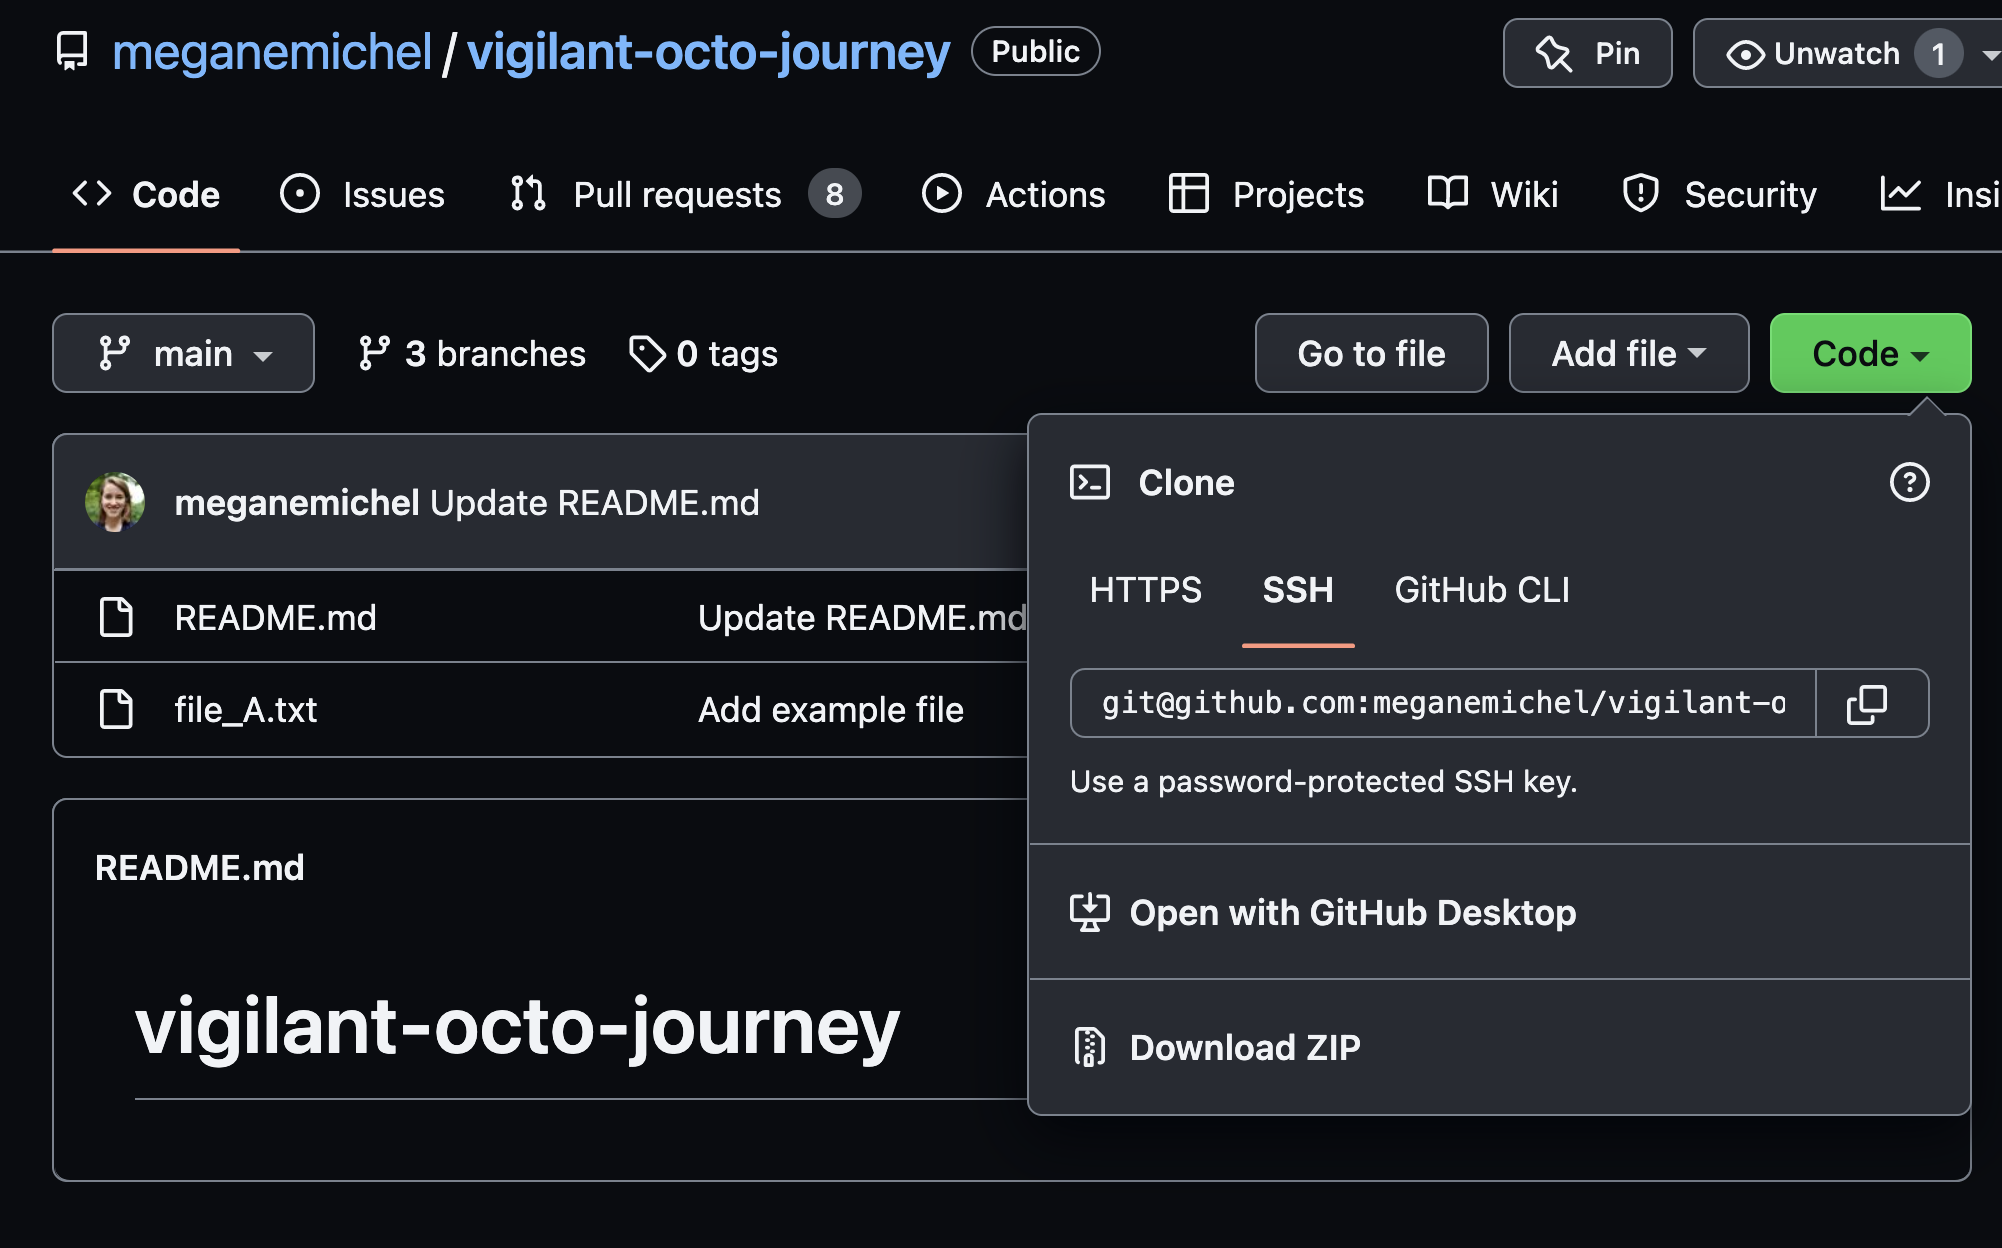
\includegraphics{assets/images/chapters/introduction-to-git/git_clone.png}

Back at your command line, clone the repo as follows:

\begin{Shaded}
\begin{Highlighting}[]
\FunctionTok{git}\NormalTok{ clone git@github.com:meganemichel/vigilant{-}octo{-}journey.git}
\end{Highlighting}
\end{Shaded}

Next, let's \textbf{add} a new or modified file to our `staging area' on
our local machine.

\begin{Shaded}
\begin{Highlighting}[]
\BuiltInTok{cd}\NormalTok{ vigilant{-}octo{-}journey}
\BuiltInTok{echo} \StringTok{"test\_file"} \OperatorTok{\textgreater{}}\NormalTok{ file\_A.txt}
\BuiltInTok{echo} \StringTok{"Just an example repo"} \OperatorTok{\textgreater{}\textgreater{}}\NormalTok{ README.md}
\FunctionTok{git}\NormalTok{ add file\_A.txt}
\end{Highlighting}
\end{Shaded}

Now we can check what files have been locally changed, staged, etc. with
\textbf{status}.

\begin{Shaded}
\begin{Highlighting}[]
\FunctionTok{git}\NormalTok{ status}
\end{Highlighting}
\end{Shaded}

You should see that \texttt{file\_A.txt} is staged to be committed, but
\texttt{README.md} is NOT. Try adding \texttt{README.md} and check the
status again.

Now we need to package or save the changes into a \textbf{commit} with a
message describing the changes we've made. Each commit comes with a
unique hash ID and will be stored forever in git history.

\begin{Shaded}
\begin{Highlighting}[]
\FunctionTok{git}\NormalTok{ commit }\AttributeTok{{-}m} \StringTok{"Add example file"}
\end{Highlighting}
\end{Shaded}

Finally, let's \textbf{push} our local commit back to our remote
repository.

\begin{Shaded}
\begin{Highlighting}[]
\FunctionTok{git}\NormalTok{ push}
\end{Highlighting}
\end{Shaded}

What if we want to download new commits from our remote to our local
repository?

\begin{Shaded}
\begin{Highlighting}[]
\FunctionTok{git}\NormalTok{ pull}
\end{Highlighting}
\end{Shaded}

You should see that your repository is already up-to-date, since we have
not made new changes to the remote repo. Let's try making a change to
the remote repository's README file (as below). Then, back on the
command line, pull the repository again.

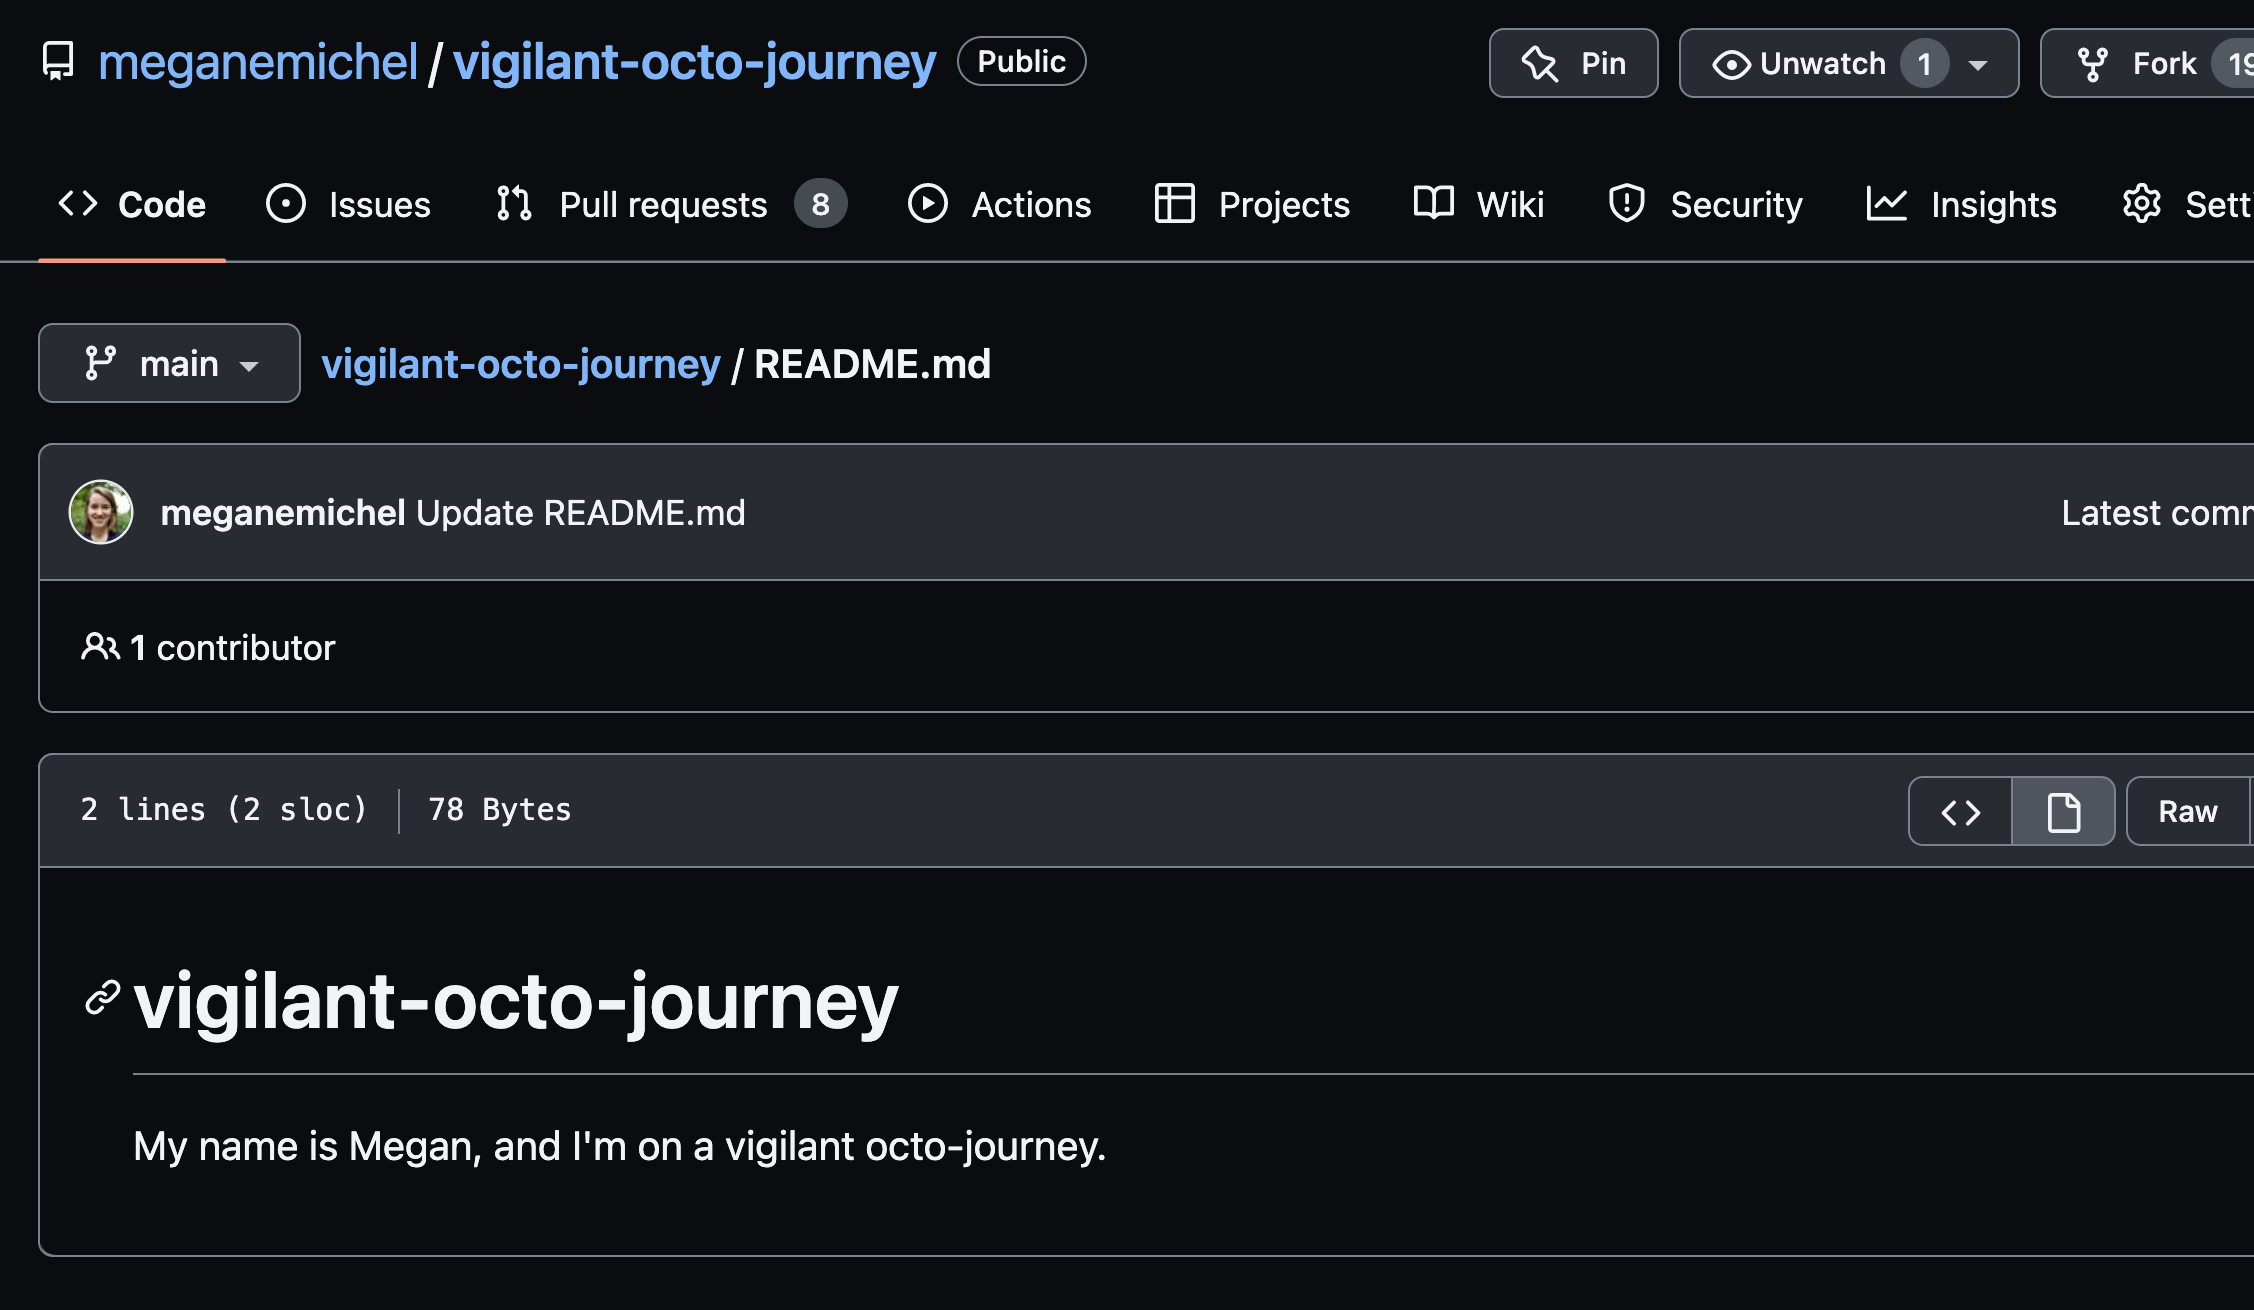
\includegraphics{assets/images/chapters/introduction-to-git/git_pull.png}

\hypertarget{working-collaboratively}{%
\section{Working collaboratively}\label{working-collaboratively}}

Github facilitates simultaneous work by small teams through branching,
which generates a copy of the main repository within the repository.
This can be edited without breaking the `master' version. First, back on
github, make a new branch of your repository.

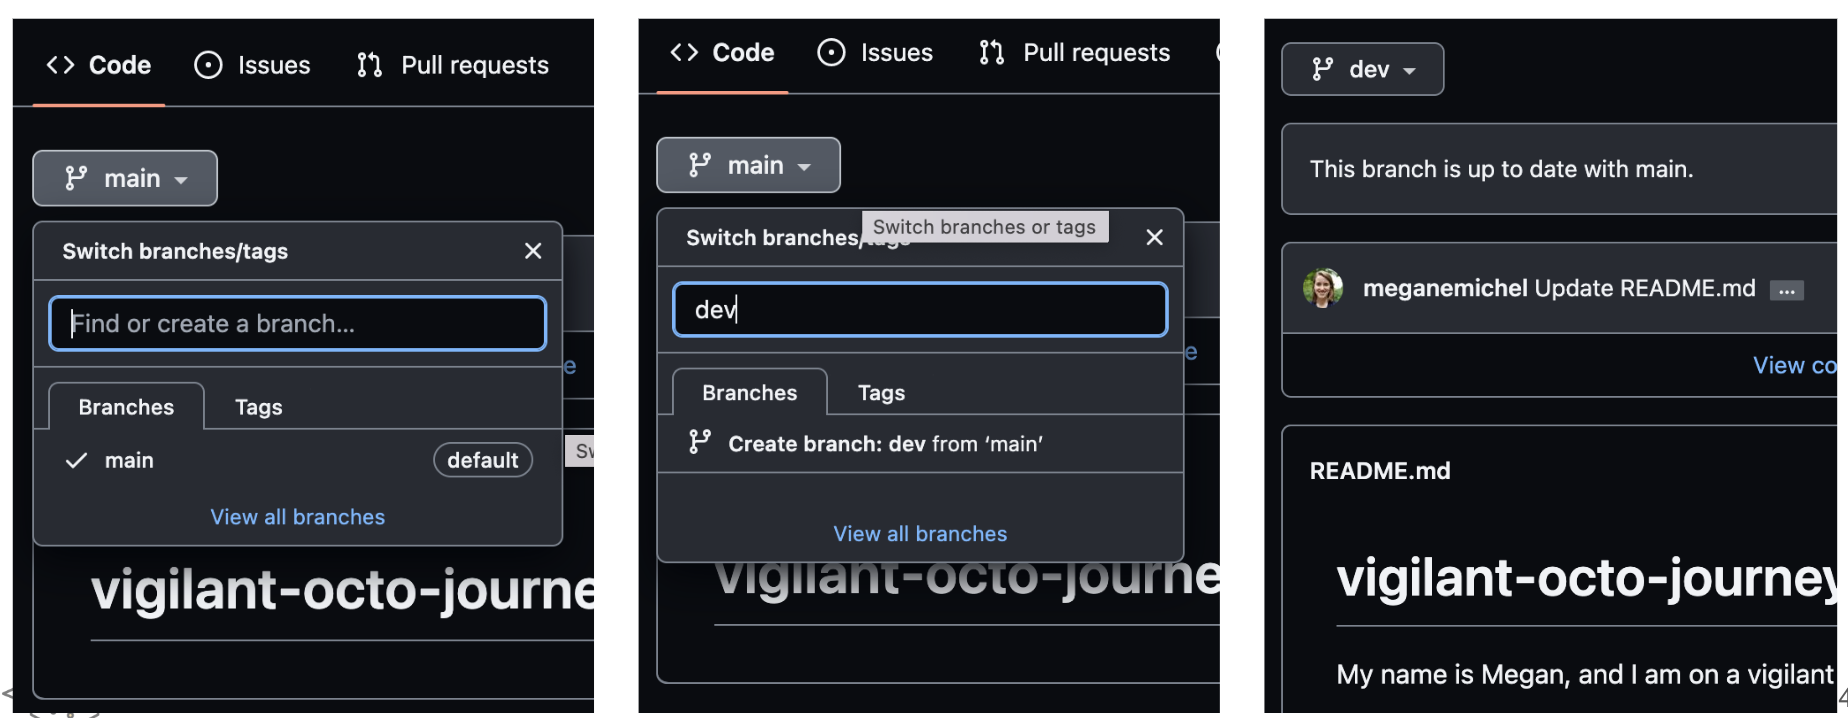
\includegraphics{assets/images/chapters/introduction-to-git/git_switch.png}

From the command line, you can create a new branch as follows:

\begin{Shaded}
\begin{Highlighting}[]
\FunctionTok{git}\NormalTok{ switch }\AttributeTok{{-}c}\NormalTok{ new\_branch}
\end{Highlighting}
\end{Shaded}

To switch back to the main branch, use

\begin{Shaded}
\begin{Highlighting}[]
\FunctionTok{git}\NormalTok{ switch main}
\end{Highlighting}
\end{Shaded}

Note that you \textbf{must commit changes} for them to be saved to the
desired branch!

\hypertarget{pull-requests}{%
\section{Pull requests}\label{pull-requests}}

A \textbf{Pull request} (aka PR) is used to propose changes to a branch
from another branch. Others can comment and make suggestinos before your
changes are merged into the main branch. For more information on
creating a pull request, see github's documentation:
\url{https://docs.github.com/en/pull-requests/collaborating-with-pull-requests/proposing-changes-to-your-work-with-pull-requests/creating-a-pull-request}.

\hypertarget{questions-to-think-about-4}{%
\section{Questions to think about}\label{questions-to-think-about-4}}

\begin{enumerate}
\def\labelenumi{\arabic{enumi}.}
\tightlist
\item
  Why is using a version control software for tracking data and code
  important?
\item
  How can using Git(Hub) help me to collaborate on group projects?
\end{enumerate}

\part{Ancient Metagenomics}

The techniques in this section of the book can be used in a variety of
stages of any ancient metagenomics projects, for screening for pathogens
(what species should I target for downstream genomic mapping?), for
differential abundance analysis (does the community make of this sample
change between different cultural periods?), but also for reference-free
assembly of genomes (can I recover the genome architecture of a variety
of species in my sample?). It focuses on the concept of `many samples to
many genomes' using high-throughput techniques and algorithms and trying
to analyse data at whole `community' levels.

\hypertarget{taxonomic-profiling}{%
\section*{\texorpdfstring{\protect\hyperlink{taxonomic-profiling-otu-tables-and-visualisation}{Taxonomic
Profiling}}{Taxonomic Profiling}}\label{taxonomic-profiling}}
\addcontentsline{toc}{section}{\protect\hyperlink{taxonomic-profiling-otu-tables-and-visualisation}{Taxonomic
Profiling}}

\markright{Taxonomic Profiling}

\emph{TBC}

\hypertarget{functional-profiling}{%
\section*{\texorpdfstring{\protect\hyperlink{functional-profiling-1}{Functional
Profiling}}{Functional Profiling}}\label{functional-profiling}}
\addcontentsline{toc}{section}{\protect\hyperlink{functional-profiling-1}{Functional
Profiling}}

\markright{Functional Profiling}

The value of microbial taxonomy lies in the implied biochemical
properties of a given taxon. Historically taxonomy was determined by
growth characteristics and cell properties, and more recently through
genomic and genetic similarity.

The genomic content of microbial taxa, specifically the presence or
absence of genes, determine how those taxa interact with their
environment, including all the biochemical processes they participate
in, both internally and externally. Strains within any microbial species
may have different genetic content and therefore may behave strikingly
differently in the same environment, which cannot be determined through
taxonomic profiling. Functionally profiling a microbial community, or
determining all of the genes present independent of the species they are
derived from, reveals the biochemical reactions and metabolic products
the community may perform and produce, respectively.

This approach may provide insights to community activity and
environmental interactions that are hidden when using taxonomic
approaches alone. In this chapter we will perform functional profiling
of metagenomic communities to assess their genetic content and inferred
metabolic pathways.

\hypertarget{de-novo-assembly}{%
\section*{\texorpdfstring{\protect\hyperlink{introduction-to-de-novo-genome-assembly}{\emph{De
novo} Assembly}}{De novo Assembly}}\label{de-novo-assembly}}
\addcontentsline{toc}{section}{\protect\hyperlink{introduction-to-de-novo-genome-assembly}{\emph{De
novo} Assembly}}

\markright{\emph{De novo} Assembly}

\emph{De novo} assembly of ancient metagenomic samples enables the
recovery of the genetic information of organisms without requiring any
prior knowledge about their genomes. Therefore, this approach is very
well suited to study the biological diversity of species that have not
been studied well or are simply not known yet.

In this chapter, we will show you how to prepare your sequencing data
and subsequently \emph{de novo} assemble them. Furthermore, we will then
learn how we can actually evaluate what organisms we might have
assembled and whether we obtained enough data to reconstruct a whole
metagenome-assembled genome. We will particularly focus on the quality
assessment of these reconstructed genomes and how we can ensure that we
obtained high-quality genomes.

\hypertarget{taxonomic-profiling-otu-tables-and-visualisation}{%
\chapter{Taxonomic Profiling, OTU Tables and
Visualisation}\label{taxonomic-profiling-otu-tables-and-visualisation}}

\begin{tcolorbox}[enhanced jigsaw, opacitybacktitle=0.6, bottomtitle=1mm, opacityback=0, colback=white, coltitle=black, leftrule=.75mm, toprule=.15mm, title=\textcolor{quarto-callout-tip-color}{\faLightbulb}\hspace{0.5em}{Tip}, colframe=quarto-callout-tip-color-frame, toptitle=1mm, arc=.35mm, left=2mm, titlerule=0mm, breakable, rightrule=.15mm, bottomrule=.15mm, colbacktitle=quarto-callout-tip-color!10!white]

For this chapter's exercises, if not already performed, you will need to
create the \protect\hyperlink{creating-a-conda-environment}{conda
environment} from the \texttt{yml} file in the following
\href{https://doi.org/10.5281/zenodo.6983165}{archive}, and activate the
environment:

\begin{Shaded}
\begin{Highlighting}[]
\ExtensionTok{conda}\NormalTok{ activate r{-}python}
\end{Highlighting}
\end{Shaded}

\end{tcolorbox}

\hypertarget{lecture-9}{%
\section{Lecture}\label{lecture-9}}

PDF version of these slides can be downloaded from
\href{https://github.com/SPAAM-community/wss-summer-school/raw/main/docs/assets/slides/2022/3c-intro-to-taxprofiling/SPAAM\%20Summer\%20School\%202022\%20-\%203C\%20-\%20Intro\%20to\%20microbial\%20ecology\%20for\%20ancient\%20DNA.pdf}{here}.

This session is run using a Jupyter notebook. This can be found
\href{https://github.com/maxibor/microbiome_tutorial}{here}. However, it
will already be installed on compute nodes during the summer school.

\begin{tcolorbox}[enhanced jigsaw, opacitybacktitle=0.6, bottomtitle=1mm, opacityback=0, colback=white, coltitle=black, leftrule=.75mm, toprule=.15mm, title=\textcolor{quarto-callout-warning-color}{\faExclamationTriangle}\hspace{0.5em}{Warning}, colframe=quarto-callout-warning-color-frame, toptitle=1mm, arc=.35mm, left=2mm, titlerule=0mm, breakable, rightrule=.15mm, bottomrule=.15mm, colbacktitle=quarto-callout-warning-color!10!white]

We highly recommend viewing this walkthrough via the Jupyter notebook
above! The output of commands on the website for this walkthrough are
displayed in their own code blocks - be wary of what you copy-paste!

\end{tcolorbox}

\hypertarget{download-and-subsample}{%
\section{Download and Subsample}\label{download-and-subsample}}

\begin{Shaded}
\begin{Highlighting}[]
\ImportTok{import}\NormalTok{ subprocess}
\ImportTok{import}\NormalTok{ glob}
\ImportTok{from}\NormalTok{ pathlib }\ImportTok{import}\NormalTok{ Path}
\end{Highlighting}
\end{Shaded}

For this tutorial, we will be using the ERR5766177 library from the
sample 2612 published by
\href{https://doi.org/10.1016/j.cub.2021.09.031}{Maixner et al.~2021}

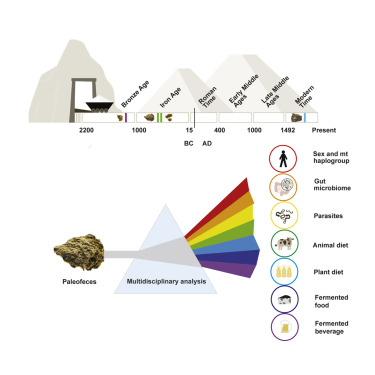
\includegraphics{assets/images/chapters/taxonomic-profiling/1-s2.0-S0960982221012719-fx1.jpg}

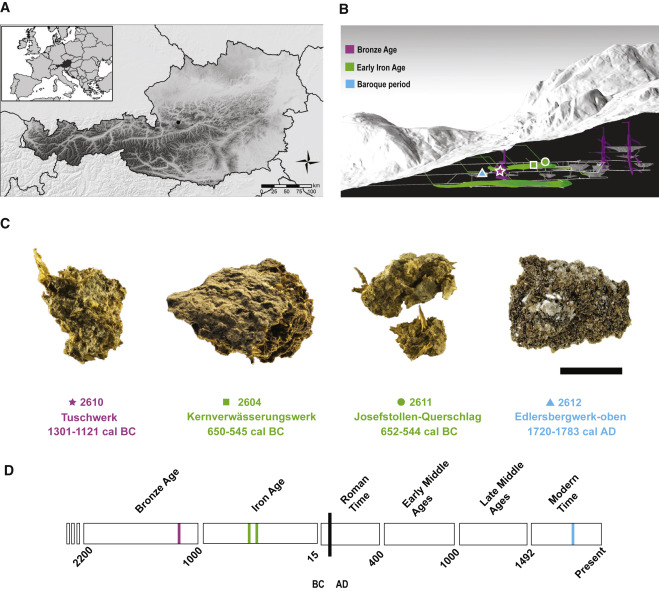
\includegraphics{assets/images/chapters/taxonomic-profiling/1-s2.0-S0960982221012719-gr1.jpg}`

\hypertarget{subsampling-the-sequencing-files-to-make-the-analysis-quicker-for-this-tutorial}{%
\subsection{Subsampling the sequencing files to make the analysis
quicker for this
tutorial}\label{subsampling-the-sequencing-files-to-make-the-analysis-quicker-for-this-tutorial}}

\begin{Shaded}
\begin{Highlighting}[]
\KeywordTok{def}\NormalTok{ subsample(filename, outdir, depth}\OperatorTok{=}\DecValTok{1000000}\NormalTok{):}
\NormalTok{    basename }\OperatorTok{=}\NormalTok{ Path(filename).stem}
\NormalTok{    cmd }\OperatorTok{=} \SpecialStringTok{f"seqtk sample {-}s42 }\SpecialCharTok{\{}\NormalTok{filename}\SpecialCharTok{\}}\SpecialStringTok{ }\SpecialCharTok{\{}\NormalTok{depth}\SpecialCharTok{\}}\SpecialStringTok{ \textgreater{} }\SpecialCharTok{\{}\NormalTok{outdir}\SpecialCharTok{\}}\SpecialStringTok{/}\SpecialCharTok{\{}\NormalTok{basename}\SpecialCharTok{\}}\SpecialStringTok{\_subsample\_}\SpecialCharTok{\{}\NormalTok{depth}\SpecialCharTok{\}}\SpecialStringTok{.fastq"}
    \BuiltInTok{print}\NormalTok{(cmd)}
\NormalTok{    subprocess.check\_output(cmd, shell}\OperatorTok{=}\VariableTok{True}\NormalTok{)}
\end{Highlighting}
\end{Shaded}

\begin{Shaded}
\begin{Highlighting}[]
\ControlFlowTok{for}\NormalTok{ f }\KeywordTok{in}\NormalTok{ glob.glob(}\StringTok{"../data/raw/*"}\NormalTok{):}
\NormalTok{    outdir }\OperatorTok{=} \StringTok{"../data/subsampled"}
\NormalTok{    subsample(f, outdir)}
\end{Highlighting}
\end{Shaded}

\begin{verbatim}
seqtk sample -s42 ../data/raw/ERR5766177_PE.mapped.hostremoved.fwd.fq.gz 1000000 >
../data/subsampled/ERR5766177_PE.mapped.hostremoved.fwd.fq_subsample_1000000.fastq
seqtk sample -s42 ../data/raw/ERR5766177_PE.mapped.hostremoved.rev.fq.gz 1000000 >
../data/subsampled/ERR5766177_PE.mapped.hostremoved.rev.fq_subsample_1000000.fastq
\end{verbatim}

\begin{Shaded}
\begin{Highlighting}[]
\OperatorTok{!}\NormalTok{ gzip }\OperatorTok{{-}}\NormalTok{f ..}\OperatorTok{/}\NormalTok{data}\OperatorTok{/}\NormalTok{subsampled}\OperatorTok{/*}\NormalTok{.fastq}
\end{Highlighting}
\end{Shaded}

\hypertarget{hands-on-introduction-to-ancient-microbiome-analysis}{%
\section{Hands on introduction to ancient microbiome
analysis}\label{hands-on-introduction-to-ancient-microbiome-analysis}}

Author: Maxime Borry\\
Date: 12/08/2021

In this tutorial, we're going to go through the steps necessary to:

\begin{itemize}
\tightlist
\item
  generate a taxonomic profile table with
  \href{https://github.com/biobakery/MetaPhlAn}{metaphlan v3.0}
\item
  have a look at metaphlan results with
  \href{https://github.com/fbreitwieser/pavian}{Pavian} and generate a
  \href{https://github.com/marbl/Krona/wiki}{Krona plot}
\item
  Compare the diversity of our samples vs the diversity of modern human
  gut samples
\item
  Compare the composition of our samples vs modern gut samples, and see
  where they fit in a lower dimensional space
\end{itemize}

\hypertarget{quick-intro-to-jupyter-notebooks}{%
\subsection{0. Quick intro to Jupyter
Notebooks}\label{quick-intro-to-jupyter-notebooks}}

This a markdown cell

\begin{Shaded}
\begin{Highlighting}[]
\BuiltInTok{print}\NormalTok{(}\StringTok{"This is a python cell"}\NormalTok{)}
\end{Highlighting}
\end{Shaded}

\begin{verbatim}
This is a python cell
\end{verbatim}

\begin{Shaded}
\begin{Highlighting}[]
\OperatorTok{!}\NormalTok{ echo }\StringTok{"This is how to run a single line bash command"}
\end{Highlighting}
\end{Shaded}

\begin{verbatim}
This is how to run a single line bash command
\end{verbatim}

\begin{Shaded}
\begin{Highlighting}[]
\ExtensionTok{\%\%bash}
\BuiltInTok{echo} \StringTok{"This how to run a multi"}
\BuiltInTok{echo} \StringTok{"lines bash command"}
\end{Highlighting}
\end{Shaded}

\begin{verbatim}
This how to run a multi
lines bash command
\end{verbatim}

\hypertarget{data-pre-processing}{%
\subsection{1. Data pre-processing}\label{data-pre-processing}}

Before starting to analyze our data, we will need to pre-process them to
remove reads mapping to the host genome, here, \emph{Homo sapiens}

To do so, I've used
\href{https://github.com/nf-core/eager}{nf-core/eager}

I've already pre-processed the data, and the resulting cleaned files are
available in the \url{data/eager_cleaned}, but the basic eager command
to do so is:

\begin{verbatim}
nextflow run nf-core/eager -profile <docker/singularity/podman/conda/institute> --input '*_R{1,2}.fastq.gz' \
--fasta 'human_genome.fasta' --hostremoval_input_fastq
\end{verbatim}

\hypertarget{adapter-sequence-trimming-and-low-quality-bases-trimming}{%
\subsection{2. Adapter sequence trimming and low-quality bases
trimming}\label{adapter-sequence-trimming-and-low-quality-bases-trimming}}

Sequencing adapters are small DNA sequences adding prior to DNA
sequencing to allow the DNA fragments to attach to the sequencing flow
cells. Because these adapters could interfere with downtstream analyses,
we need to remove them before proceeding any further. Furthermore,
because the quality of the sequencing is not always optimal, we need to
remove bases of lower sequencing quality to might lead to spurious
results in downstream analyses.

To perform both of these tasks, we'll use the program
\href{https://github.com/OpenGene/fastp}{fastp}.

\begin{Shaded}
\begin{Highlighting}[]
\OperatorTok{!}\NormalTok{ fastp }\OperatorTok{{-}}\NormalTok{h}
\end{Highlighting}
\end{Shaded}

\begin{verbatim}
option needs value: --html
usage: fastp [options] ...
options:
  -i, --in1                            read1 input file name (string [=])
  -o, --out1                           read1 output file name (string [=])
  -I, --in2                            read2 input file name (string [=])
  -O, --out2                           read2 output file name (string [=])
      --unpaired1                      for PE input, if read1 passed QC but read2 not, it will be written to unpaired1.
                                       Default is to discard it. (string [=])
      --unpaired2                      for PE input, if read2 passed QC but read1 not, it will be written to unpaired2.
                                       If --unpaired2 is same as --unpaired1 (default mode), both unpaired reads will be
                                       written to this same file. (string [=])
      --overlapped_out                 for each read pair, output the overlapped region if it has no any mismatched
                                       base. (string [=])
      --failed_out                     specify the file to store reads that cannot pass the filters. (string [=])
  -m, --merge                          for paired-end input, merge each pair of reads into a single read if they are
                                       overlapped. The merged reads will be written
                                       to the file given by --merged_out, the unmerged reads will be written to the
                                       files specified by --out1 and --out2. The merging mode is disabled by default.
      --merged_out                     in the merging mode, specify the file name to store merged output, or specify
                                       --stdout to stream the merged output (string [=])
      --include_unmerged               in the merging mode, write the unmerged or unpaired reads to the file specified
                                       by --merge. Disabled by default.
  -6, --phred64                        indicate the input is using phred64 scoring (it'll be converted to phred33,
                                       so the output will still be phred33)
  -z, --compression                    compression level for gzip output (1 ~ 9). 1 is fastest, 9 is smallest, default is 4. (int [=4])
      --stdin                          input from STDIN. If the STDIN is interleaved paired-end FASTQ, please also add --interleaved_in.
      --stdout                         stream passing-filters reads to STDOUT. This option will result in interleaved
                                       FASTQ output for paired-end output. Disabled by default.
      --interleaved_in                 indicate that <in1> is an interleaved FASTQ which contains both read1 and read2.
                                       Disabled by default.
      --reads_to_process               specify how many reads/pairs to be processed. Default 0 means process all reads. (int [=0])
      --dont_overwrite                 don't overwrite existing files. Overwritting is allowed by default.
      --fix_mgi_id                     the MGI FASTQ ID format is not compatible with many BAM operation tools, enable this option to fix it.
  -V, --verbose                        output verbose log information (i.e. when every 1M reads are processed).
  -A, --disable_adapter_trimming       adapter trimming is enabled by default. If this option is specified, adapter trimming is disabled
  -a, --adapter_sequence               the adapter for read1. For SE data, if not specified, the adapter will be auto-detected.
                                       For PE data, this is used if R1/R2 are found not overlapped. (string [=auto])
      --adapter_sequence_r2            the adapter for read2 (PE data only). This is used if R1/R2 are found not overlapped.
                                       If not specified, it will be the same as <adapter_sequence> (string [=auto])
      --adapter_fasta                  specify a FASTA file to trim both read1 and read2 (if PE) by all the sequences in this FASTA file (string [=])
      --detect_adapter_for_pe          by default, the auto-detection for adapter is for SE data input only, turn on this
                                    option to enable it for PE data.
  -f, --trim_front1                    trimming how many bases in front for read1, default is 0 (int [=0])
  -t, --trim_tail1                     trimming how many bases in tail for read1, default is 0 (int [=0])
  -b, --max_len1                       if read1 is longer than max_len1, then trim read1 at its tail to make it as
                                       long as max_len1. Default 0 means no limitation (int [=0])
  -F, --trim_front2                    trimming how many bases in front for read2. If it's not specified, it will follow read1's settings (int [=0])
  -T, --trim_tail2                     trimming how many bases in tail for read2. If it's not specified, it will follow read1's settings (int [=0])
  -B, --max_len2                       if read2 is longer than max_len2, then trim read2 at its tail to make it as long as max_len2.
                                       Default 0 means no limitation. If it's not specified, it will follow read1's settings (int [=0])
  -D, --dedup                          enable deduplication to drop the duplicated reads/pairs
      --dup_calc_accuracy              accuracy level to calculate duplication (1~6), higher level uses more memory (1G, 2G, 4G, 8G, 16G, 24G).
                                       Default 1 for no-dedup mode, and 3 for dedup mode. (int [=0])
      --dont_eval_duplication          don't evaluate duplication rate to save time and use less memory.
  -g, --trim_poly_g                    force polyG tail trimming, by default trimming is automatically enabled for Illumina NextSeq/NovaSeq data
      --poly_g_min_len                 the minimum length to detect polyG in the read tail. 10 by default. (int [=10])
  -G, --disable_trim_poly_g            disable polyG tail trimming, by default trimming is automatically enabled for Illumina NextSeq/NovaSeq data
  -x, --trim_poly_x                    enable polyX trimming in 3' ends.
      --poly_x_min_len                 the minimum length to detect polyX in the read tail. 10 by default. (int [=10])
  -5, --cut_front                      move a sliding window from front (5') to tail, drop the bases in the window if
                                       its mean quality < threshold, stop otherwise.
  -3, --cut_tail                       move a sliding window from tail (3') to front, drop the bases in the window if
                                       its mean quality < threshold, stop otherwise.
  -r, --cut_right                      move a sliding window from front to tail, if meet one window with mean quality
                                       < threshold, drop the bases in the window and the right part, and then stop.
  -W, --cut_window_size                the window size option shared by cut_front, cut_tail or cut_sliding. Range: 1~1000, default: 4 (int [=4])
  -M, --cut_mean_quality               the mean quality requirement option shared by cut_front, cut_tail or cut_sliding.
                                       Range: 1~36 default: 20 (Q20) (int [=20])
      --cut_front_window_size          the window size option of cut_front, default to cut_window_size if not specified (int [=4])
      --cut_front_mean_quality         the mean quality requirement option for cut_front, default to cut_mean_quality if not specified (int [=20])
      --cut_tail_window_size           the window size option of cut_tail, default to cut_window_size if not specified (int [=4])
      --cut_tail_mean_quality          the mean quality requirement option for cut_tail, default to cut_mean_quality if not specified (int [=20])
      --cut_right_window_size          the window size option of cut_right, default to cut_window_size if not specified (int [=4])
      --cut_right_mean_quality         the mean quality requirement option for cut_right, default to cut_mean_quality if not specified (int [=20])
  -Q, --disable_quality_filtering      quality filtering is enabled by default. If this option is specified, quality filtering is disabled
  -q, --qualified_quality_phred        the quality value that a base is qualified. Default 15 means phred quality >=Q15 is qualified. (int [=15])
  -u, --unqualified_percent_limit      how many percents of bases are allowed to be unqualified (0~100). Default 40 means 40% (int [=40])
  -n, --n_base_limit                   if one read's number of N base is >n_base_limit, then this read/pair is discarded. Default is 5 (int [=5])
  -e, --average_qual                   if one read's average quality score <avg_qual, then this read/pair is discarded.
                                       Default 0 means no requirement (int [=0])
  -L, --disable_length_filtering       length filtering is enabled by default. If this option is specified, length filtering is disabled
  -l, --length_required                reads shorter than length_required will be discarded, default is 15. (int [=15])
      --length_limit                   reads longer than length_limit will be discarded, default 0 means no limitation. (int [=0])
  -y, --low_complexity_filter          enable low complexity filter. The complexity is defined as the percentage of base
                                       that is different from its next base (base[i] != base[i+1]).
  -Y, --complexity_threshold           the threshold for low complexity filter (0~100). Default is 30, which means 30% complexity is required. (int [=30])
      --filter_by_index1               specify a file contains a list of barcodes of index1 to be filtered out, one barcode per line (string [=])
      --filter_by_index2               specify a file contains a list of barcodes of index2 to be filtered out, one barcode per line (string [=])
      --filter_by_index_threshold      the allowed difference of index barcode for index filtering, default 0 means completely identical. (int [=0])
  -c, --correction                     enable base correction in overlapped regions (only for PE data), default is disabled
      --overlap_len_require            the minimum length to detect overlapped region of PE reads. This will affect overlap analysis based PE merge,
                                       adapter trimming and correction. 30 by default. (int [=30])
      --overlap_diff_limit             the maximum number of mismatched bases to detect overlapped region of PE reads.
                                       This will affect overlap analysis based PE merge, adapter trimming and correction. 5 by default. (int [=5])
      --overlap_diff_percent_limit     the maximum percentage of mismatched bases to detect overlapped region of PE reads.
                                       This will affect overlap analysis based PE merge, adapter trimming and correction. Default 20 means 20%. (int [=20])
  -U, --umi                            enable unique molecular identifier (UMI) preprocessing
      --umi_loc                        specify the location of UMI, can be (index1/index2/read1/read2/per_index/per_read, default is none (string [=])
      --umi_len                        if the UMI is in read1/read2, its length should be provided (int [=0])
      --umi_prefix                     if specified, an underline will be used to connect prefix and UMI (i.e.
                                       prefix=UMI, UMI=AATTCG, final=UMI_AATTCG). No prefix by default (string [=])
      --umi_skip                       if the UMI is in read1/read2, fastp can skip several bases following UMI, default is 0 (int [=0])
  -p, --overrepresentation_analysis    enable overrepresented sequence analysis.
  -P, --overrepresentation_sampling    one in (--overrepresentation_sampling) reads will be computed for overrepresentation
                                       analysis (1~10000), smaller is slower, default is 20. (int [=20])
  -j, --json                           the json format report file name (string [=fastp.json])
  -h, --html                           the html format report file name (string [=fastp.html])
  -R, --report_title                   should be quoted with ' or ", default is "fastp report" (string [=fastp report])
  -w, --thread                         worker thread number, default is 3 (int [=3])
  -s, --split                          split output by limiting total split file number with this option (2~999), a sequential number prefix
                                       will be added to output name ( 0001.out.fq, 0002.out.fq...), disabled by default (int [=0])
  -S, --split_by_lines                 split output by limiting lines of each file with this option(>=1000), a sequential number prefix will be
                                       added to output name ( 0001.out.fq, 0002.out.fq...), disabled by default (long [=0])
  -d, --split_prefix_digits            the digits for the sequential number padding (1~10), default is 4, so the filename will be padded as
                                       0001.xxx, 0 to disable padding (int [=4])
      --cut_by_quality5                DEPRECATED, use --cut_front instead.
      --cut_by_quality3                DEPRECATED, use --cut_tail instead.
      --cut_by_quality_aggressive      DEPRECATED, use --cut_right instead.
      --discard_unmerged               DEPRECATED, no effect now, see the introduction for merging.
  -?, --help                           print this message
\end{verbatim}

\begin{Shaded}
\begin{Highlighting}[]
\ExtensionTok{\%\%bash}
\ExtensionTok{fastp} \DataTypeTok{\textbackslash{}}
    \AttributeTok{{-}{-}in1}\NormalTok{ ../data/subsampled/ERR5766177\_PE.mapped.hostremoved.fwd.fq\_subsample\_1000000.fastq.gz }\DataTypeTok{\textbackslash{}}
    \AttributeTok{{-}{-}in2}\NormalTok{ ../data/subsampled/ERR5766177\_PE.mapped.hostremoved.fwd.fq\_subsample\_1000000.fastq.gz }\DataTypeTok{\textbackslash{}}
    \AttributeTok{{-}{-}merge} \DataTypeTok{\textbackslash{}}
    \AttributeTok{{-}{-}merged\_out}\NormalTok{ ../results/fastp/ERR5766177.merged.fastq.gz }\DataTypeTok{\textbackslash{}}
    \AttributeTok{{-}{-}include\_unmerged} \DataTypeTok{\textbackslash{}}
    \AttributeTok{{-}{-}dedup} \DataTypeTok{\textbackslash{}}
    \AttributeTok{{-}{-}json}\NormalTok{ ../results/fastp/ERR5766177.fastp.json }\DataTypeTok{\textbackslash{}}
    \AttributeTok{{-}{-}html}\NormalTok{ ../results/fastp/ERR5766177.fastp.html }\DataTypeTok{\textbackslash{}}
\end{Highlighting}
\end{Shaded}

\begin{verbatim}
Read1 before filtering:
total reads: 1000000
total bases: 101000000
Q20 bases: 99440729(98.4562%)
Q30 bases: 94683150(93.7457%)

Read2 before filtering:
total reads: 1000000
total bases: 101000000
Q20 bases: 99440729(98.4562%)
Q30 bases: 94683150(93.7457%)

Merged and filtered:
total reads: 1994070
total bases: 201397311
Q20 bases: 198330392(98.4772%)
Q30 bases: 188843169(93.7665%)

Filtering result:
reads passed filter: 1999252
reads failed due to low quality: 728
reads failed due to too many N: 20
reads failed due to too short: 0
reads with adapter trimmed: 282
bases trimmed due to adapters: 18654
reads corrected by overlap analysis: 0
bases corrected by overlap analysis: 0

Duplication rate: 0.2479%

Insert size peak (evaluated by paired-end reads): 31

Read pairs merged: 228
% of original read pairs: 0.0228%
% in reads after filtering: 0.0114339%


JSON report: ../results/fastp/ERR5766177.fastp.json
HTML report: ../results/fastp/ERR5766177.fastp.html

fastp --in1 ../data/subsampled/ERR5766177_PE.mapped.hostremoved.fwd.fq_subsample_1000000.fastq.gz \
--in2 ../data/subsampled/ERR5766177_PE.mapped.hostremoved.fwd.fq_subsample_1000000.fastq.gz --merge \
--merged_out ../results/fastp/ERR5766177.merged.fastq.gz --include_unmerged --dedup \
--json ../results/fastp/ERR5766177.fastp.json --html ../results/fastp/ERR5766177.fastp.html
fastp v0.23.2, time used: 11 seconds
\end{verbatim}

\hypertarget{taxonomic-profiling-with-metaphlan}{%
\paragraph{3. Taxonomic profiling with
Metaphlan}\label{taxonomic-profiling-with-metaphlan}}

\begin{Shaded}
\begin{Highlighting}[]
\OperatorTok{!}\NormalTok{ metaphlan  }\OperatorTok{{-}{-}}\BuiltInTok{help}
\end{Highlighting}
\end{Shaded}

\begin{verbatim}
usage: metaphlan --input_type {fastq,fasta,bowtie2out,sam} [--force]
                 [--bowtie2db METAPHLAN_BOWTIE2_DB] [-x INDEX]
                 [--bt2_ps BowTie2 presets] [--bowtie2_exe BOWTIE2_EXE]
                 [--bowtie2_build BOWTIE2_BUILD] [--bowtie2out FILE_NAME]
                 [--min_mapq_val MIN_MAPQ_VAL] [--no_map] [--tmp_dir]
                 [--tax_lev TAXONOMIC_LEVEL] [--min_cu_len]
                 [--min_alignment_len] [--add_viruses] [--ignore_eukaryotes]
                 [--ignore_bacteria] [--ignore_archaea] [--stat_q]
                 [--perc_nonzero] [--ignore_markers IGNORE_MARKERS]
                 [--avoid_disqm] [--stat] [-t ANALYSIS TYPE]
                 [--nreads NUMBER_OF_READS] [--pres_th PRESENCE_THRESHOLD]
                 [--clade] [--min_ab] [-o output file] [--sample_id_key name]
                 [--use_group_representative] [--sample_id value]
                 [-s sam_output_file] [--legacy-output] [--CAMI_format_output]
                 [--unknown_estimation] [--biom biom_output] [--mdelim mdelim]
                 [--nproc N] [--install] [--force_download]
                 [--read_min_len READ_MIN_LEN] [-v] [-h]
                 [INPUT_FILE] [OUTPUT_FILE]

DESCRIPTION
 MetaPhlAn version 3.1.0 (25 Jul 2022):
 METAgenomic PHyLogenetic ANalysis for metagenomic taxonomic profiling.

AUTHORS: Francesco Beghini (francesco.beghini@unitn.it),Nicola Segata (nicola.segata@unitn.it), Duy Tin Truong,
Francesco Asnicar (f.asnicar@unitn.it), Aitor Blanco Miguez (aitor.blancomiguez@unitn.it)

COMMON COMMANDS

 We assume here that MetaPhlAn is installed using the several options available (pip, conda, PyPi)
 Also BowTie2 should be in the system path with execution and read permissions, and Perl should be installed)

========== MetaPhlAn clade-abundance estimation =================

The basic usage of MetaPhlAn consists in the identification of the clades (from phyla to species )
present in the metagenome obtained from a microbiome sample and their
relative abundance. This correspond to the default analysis type (-t rel_ab).

*  Profiling a metagenome from raw reads:
$ metaphlan metagenome.fastq --input_type fastq -o profiled_metagenome.txt

*  You can take advantage of multiple CPUs and save the intermediate BowTie2 output for re-running
   MetaPhlAn extremely quickly:
$ metaphlan metagenome.fastq --bowtie2out metagenome.bowtie2.bz2 --nproc 5 --input_type fastq -o profiled_metagenome.txt

*  If you already mapped your metagenome against the marker DB (using a previous MetaPhlAn run), you
   can obtain the results in few seconds by using the previously saved --bowtie2out file and
   specifying the input (--input_type bowtie2out):
$ metaphlan metagenome.bowtie2.bz2 --nproc 5 --input_type bowtie2out -o profiled_metagenome.txt

*  bowtie2out files generated with MetaPhlAn versions below 3 are not compatibile.
   Starting from MetaPhlAn 3.0, the BowTie2 ouput now includes the size of the profiled metagenome and the average read length.
   If you want to re-run MetaPhlAn using these file you should provide the metagenome size via --nreads:
$ metaphlan metagenome.bowtie2.bz2 --nproc 5 --input_type bowtie2out --nreads 520000 -o profiled_metagenome.txt

*  You can also provide an externally BowTie2-mapped SAM if you specify this format with
   --input_type. Two steps: first apply BowTie2 and then feed MetaPhlAn with the obtained sam:
$ bowtie2 --sam-no-hd --sam-no-sq --no-unal --very-sensitive -S metagenome.sam -x \
  ${mpa_dir}/metaphlan_databases/mpa_v30_CHOCOPhlAn_201901 -U metagenome.fastq
$ metaphlan metagenome.sam --input_type sam -o profiled_metagenome.txt

*  We can also natively handle paired-end metagenomes, and, more generally, metagenomes stored in
  multiple files (but you need to specify the --bowtie2out parameter):
$ metaphlan metagenome_1.fastq,metagenome_2.fastq --bowtie2out metagenome.bowtie2.bz2 --nproc 5 --input_type fastq

-------------------------------------------------------------------


========== Marker level analysis ============================

MetaPhlAn introduces the capability of characterizing organisms at the strain level using non
aggregated marker information. Such capability comes with several slightly different flavours and
are a way to perform strain tracking and comparison across multiple samples.
Usually, MetaPhlAn is first ran with the default -t to profile the species present in
the community, and then a strain-level profiling can be performed to zoom-in into specific species
of interest. This operation can be performed quickly as it exploits the --bowtie2out intermediate
file saved during the execution of the default analysis type.

*  The following command will output the abundance of each marker with a RPK (reads per kilo-base)
   higher 0.0. (we are assuming that metagenome_outfmt.bz2 has been generated before as
   shown above).
$ metaphlan -t marker_ab_table metagenome_outfmt.bz2 --input_type bowtie2out -o marker_abundance_table.txt
   The obtained RPK can be optionally normalized by the total number of reads in the metagenome
   to guarantee fair comparisons of abundances across samples. The number of reads in the metagenome
   needs to be passed with the '--nreads' argument

*  The list of markers present in the sample can be obtained with '-t marker_pres_table'
$ metaphlan -t marker_pres_table metagenome_outfmt.bz2 --input_type bowtie2out -o marker_abundance_table.txt
   The --pres_th argument (default 1.0) set the minimum RPK value to consider a marker present

*  The list '-t clade_profiles' analysis type reports the same information of '-t marker_ab_table'
   but the markers are reported on a clade-by-clade basis.
$ metaphlan -t clade_profiles metagenome_outfmt.bz2 --input_type bowtie2out -o marker_abundance_table.txt

*  Finally, to obtain all markers present for a specific clade and all its subclades, the
   '-t clade_specific_strain_tracker' should be used. For example, the following command
   is reporting the presence/absence of the markers for the B. fragilis species and its strains
   the optional argument --min_ab specifies the minimum clade abundance for reporting the markers

$ metaphlan -t clade_specific_strain_tracker --clade s__Bacteroides_fragilis metagenome_outfmt.bz2 --input_typ
  bowtie2out -o marker_abundance_table.txt

-------------------------------------------------------------------

positional arguments:
  INPUT_FILE            the input file can be:
                        * a fastq file containing metagenomic reads
                        OR
                        * a BowTie2 produced SAM file.
                        OR
                        * an intermediary mapping file of the metagenome generated by a previous MetaPhlAn run
                        If the input file is missing, the script assumes that the input is provided using the standard
                        input, or named pipes.
                        IMPORTANT: the type of input needs to be specified with --input_type
  OUTPUT_FILE           the tab-separated output file of the predicted taxon relative abundances
                        [stdout if not present]

Required arguments:
  --input_type {fastq,fasta,bowtie2out,sam}
                        set whether the input is the FASTA file of metagenomic reads or
                        the SAM file of the mapping of the reads against the MetaPhlAn db.

Mapping arguments:
  --force               Force profiling of the input file by removing the bowtie2out file
  --bowtie2db METAPHLAN_BOWTIE2_DB
                        Folder containing the MetaPhlAn database. You can specify the location by exporting the
                        DEFAULT_DB_FOLDER variable in the shell.
                        [default /Users/maxime/mambaforge/envs/summer_school_microbiome/lib/python3.9/site-packages/metaphlan/metaphlan_databases]
  -x INDEX, --index INDEX
                        Specify the id of the database version to use. If "latest", MetaPhlAn will get the latest version.
                        If an index name is provided, MetaPhlAn will try to use it, if available, and skip the online check.
                        If the database files are not found on the local MetaPhlAn installation they
                        will be automatically downloaded [default latest]
  --bt2_ps BowTie2 presets
                        Presets options for BowTie2 (applied only when a FASTA file is provided)
                        The choices enabled in MetaPhlAn are:
                         * sensitive
                         * very-sensitive
                         * sensitive-local
                         * very-sensitive-local
                        [default very-sensitive]
  --bowtie2_exe BOWTIE2_EXE
                        Full path and name of the BowTie2 executable. This option allowsMetaPhlAn to reach the
                        executable even when it is not in the system PATH or the system PATH is unreachable
  --bowtie2_build BOWTIE2_BUILD
                        Full path to the bowtie2-build command to use, deafult assumes that 'bowtie2-build is present in the system path
  --bowtie2out FILE_NAME
                        The file for saving the output of BowTie2
  --min_mapq_val MIN_MAPQ_VAL
                        Minimum mapping quality value (MAPQ) [default 5]
  --no_map              Avoid storing the --bowtie2out map file
  --tmp_dir             The folder used to store temporary files [default is the OS dependent tmp dir]

Post-mapping arguments:
  --tax_lev TAXONOMIC_LEVEL
                        The taxonomic level for the relative abundance output:
                        'a' : all taxonomic levels
                        'k' : kingdoms
                        'p' : phyla only
                        'c' : classes only
                        'o' : orders only
                        'f' : families only
                        'g' : genera only
                        's' : species only
                        [default 'a']
  --min_cu_len          minimum total nucleotide length for the markers in a clade for
                        estimating the abundance without considering sub-clade abundances
                        [default 2000]
  --min_alignment_len   The sam records for aligned reads with the longest subalignment
                        length smaller than this threshold will be discarded.
                        [default None]
  --add_viruses         Allow the profiling of viral organisms
  --ignore_eukaryotes   Do not profile eukaryotic organisms
  --ignore_bacteria     Do not profile bacterial organisms
  --ignore_archaea      Do not profile archeal organisms
  --stat_q              Quantile value for the robust average
                        [default 0.2]
  --perc_nonzero        Percentage of markers with a non zero relative abundance for misidentify a species
                        [default 0.33]
  --ignore_markers IGNORE_MARKERS
                        File containing a list of markers to ignore.
  --avoid_disqm         Deactivate the procedure of disambiguating the quasi-markers based on the
                        marker abundance pattern found in the sample. It is generally recommended
                        to keep the disambiguation procedure in order to minimize false positives
  --stat                Statistical approach for converting marker abundances into clade abundances
                        'avg_g'  : clade global (i.e. normalizing all markers together) average
                        'avg_l'  : average of length-normalized marker counts
                        'tavg_g' : truncated clade global average at --stat_q quantile
                        'tavg_l' : truncated average of length-normalized marker counts (at --stat_q)
                        'wavg_g' : winsorized clade global average (at --stat_q)
                        'wavg_l' : winsorized average of length-normalized marker counts (at --stat_q)
                        'med'    : median of length-normalized marker counts
                        [default tavg_g]

Additional analysis types and arguments:
  -t ANALYSIS TYPE      Type of analysis to perform:
                         * rel_ab: profiling a metagenomes in terms of relative abundances
                         * rel_ab_w_read_stats: profiling a metagenomes in terms of relative abundances and estimate
                                                the number of reads coming from each clade.
                         * reads_map: mapping from reads to clades (only reads hitting a marker)
                         * clade_profiles: normalized marker counts for clades with at least a non-null marker
                         * marker_ab_table: normalized marker counts (only when > 0.0 and normalized by metagenome size if --nreads is specified)
                         * marker_counts: non-normalized marker counts [use with extreme caution]
                         * marker_pres_table: list of markers present in the sample (threshold at 1.0 if not differently specified with --pres_th
                         * clade_specific_strain_tracker: list of markers present for a specific clade, specified with --clade, and all its subclades
                        [default 'rel_ab']
  --nreads NUMBER_OF_READS
                        The total number of reads in the original metagenome. It is used only when
                        -t marker_table is specified for normalizing the length-normalized counts
                        with the metagenome size as well. No normalization applied if --nreads is not
                        specified
  --pres_th PRESENCE_THRESHOLD
                        Threshold for calling a marker present by the -t marker_pres_table option
  --clade               The clade for clade_specific_strain_tracker analysis
  --min_ab              The minimum percentage abundance for the clade in the clade_specific_strain_tracker analysis

Output arguments:
  -o output file, --output_file output file
                        The output file (if not specified as positional argument)
  --sample_id_key name  Specify the sample ID key for this analysis. Defaults to 'SampleID'.
  --use_group_representative
                        Use a species as representative for species groups.
  --sample_id value     Specify the sample ID for this analysis. Defaults to 'Metaphlan_Analysis'.
  -s sam_output_file, --samout sam_output_file
                        The sam output file
  --legacy-output       Old MetaPhlAn2 two columns output
  --CAMI_format_output  Report the profiling using the CAMI output format
  --unknown_estimation  Scale relative abundances to the number of reads mapping to known clades in order to estimate unknowness
  --biom biom_output, --biom_output_file biom_output
                        If requesting biom file output: The name of the output file in biom format
  --mdelim mdelim, --metadata_delimiter_char mdelim
                        Delimiter for bug metadata: - defaults to pipe. e.g. the pipe in k__Bacteria|p__Proteobacteria

Other arguments:
  --nproc N             The number of CPUs to use for parallelizing the mapping [default 4]
  --install             Only checks if the MetaPhlAn DB is installed and installs it if not. All other parameters are ignored.
  --force_download      Force the re-download of the latest MetaPhlAn database.
  --read_min_len READ_MIN_LEN
                        Specify the minimum length of the reads to be considered when parsing the input file with
                        'read_fastx.py' script, default value is 70
  -v, --version         Prints the current MetaPhlAn version and exit
  -h, --help            show this help message and exit
\end{verbatim}

\begin{Shaded}
\begin{Highlighting}[]
\ExtensionTok{metaphlan}\NormalTok{ ../results/fastp/ERR5766177.merged.fastq.gz  }\DataTypeTok{\textbackslash{}}
    \AttributeTok{{-}{-}input\_type}\NormalTok{ fastq }\DataTypeTok{\textbackslash{}}
    \AttributeTok{{-}{-}bowtie2out}\NormalTok{ ../results/metaphlan/ERR5766177.bt2.out  }\DataTypeTok{\textbackslash{}}
    \AttributeTok{{-}{-}nproc}\NormalTok{ 4 }\DataTypeTok{\textbackslash{}}
    \OperatorTok{\textgreater{}}\NormalTok{ ../results/metaphlan/ERR5766177.metaphlan\_profile.txt}
\end{Highlighting}
\end{Shaded}

The main results files that we're interested in is located at
\url{../results/metaphlan/ERR5766177.metaphlan_profile.txt}

It's a tab separated file, with taxons in rows, with their relative
abundance in the sample

\begin{Shaded}
\begin{Highlighting}[]
\OperatorTok{!}\NormalTok{ head ..}\OperatorTok{/}\NormalTok{results}\OperatorTok{/}\NormalTok{metaphlan}\OperatorTok{/}\NormalTok{ERR5766177.metaphlan\_profile.txt}
\end{Highlighting}
\end{Shaded}

\begin{verbatim}
#mpa_v30_CHOCOPhlAn_201901
#/home/maxime_borry/.conda/envs/maxime/envs/summer_school_microbiome/bin/metaphlan ../results/fastp/ERR5766177.merged.fastq.gz \
--input_type fastq --bowtie2out ../results/metaphlan/ERR5766177.bt2.out --nproc 8
#SampleID   Metaphlan_Analysis
#clade_name NCBI_tax_id relative_abundance  additional_species
k__Bacteria 2   82.23198
k__Archaea  2157    17.76802
k__Bacteria|p__Firmicutes   2|1239  33.47957
k__Bacteria|p__Bacteroidetes    2|976   28.4209
k__Bacteria|p__Actinobacteria   2|201174    20.33151
k__Archaea|p__Euryarchaeota 2157|28890  17.76802
\end{verbatim}

\hypertarget{visualizing-the-taxonomic-profile}{%
\subsection{4. Visualizing the taxonomic
profile}\label{visualizing-the-taxonomic-profile}}

\hypertarget{visualizing-metaphlan-taxonomic-profile-with-pavian}{%
\subsubsection{4.1 Visualizing metaphlan taxonomic profile with
Pavian}\label{visualizing-metaphlan-taxonomic-profile-with-pavian}}

\href{https://github.com/fbreitwieser/pavian}{Pavian} is an interactive
app to explore results of different taxonomic classifiers

There are different ways to run it:

\begin{itemize}
\tightlist
\item
  If you have \href{https://www.docker.com/}{docker} installed (and are
  somehow familiar with it)
\end{itemize}

\begin{Shaded}
\begin{Highlighting}[]
\ExtensionTok{docker}\NormalTok{ pull }\StringTok{\textquotesingle{}florianbw/pavian\textquotesingle{}}
\ExtensionTok{docker}\NormalTok{ run }\AttributeTok{{-}{-}rm} \AttributeTok{{-}p}\NormalTok{ 5000:80 florianbw/pavian}
\end{Highlighting}
\end{Shaded}

Then open your browser and visit \url{localhost:5000}

\begin{itemize}
\tightlist
\item
  If you are familiar with \href{https://www.r-project.org/}{R}
\end{itemize}

\begin{Shaded}
\begin{Highlighting}[]
\ControlFlowTok{if}\NormalTok{ (}\SpecialCharTok{!}\FunctionTok{require}\NormalTok{(remotes)) \{ }\FunctionTok{install.packages}\NormalTok{(}\StringTok{"remotes"}\NormalTok{) \}}
\NormalTok{remotes}\SpecialCharTok{::}\FunctionTok{install\_github}\NormalTok{(}\StringTok{"fbreitwieser/pavian"}\NormalTok{)}

\NormalTok{pavian}\SpecialCharTok{::}\FunctionTok{runApp}\NormalTok{(}\AttributeTok{port=}\DecValTok{5000}\NormalTok{)}
\end{Highlighting}
\end{Shaded}

Then open your browser and visit \url{localhost:5000}

\begin{itemize}
\tightlist
\item
  Otherwise, just visit
  \href{https://fbreitwieser.shinyapps.io/pavian/.}{fbreitwieser.shinyapps.io/pavian}.
\end{itemize}

\hypertarget{visualizing-metaphlan-taxonomic-profile-with-krona}{%
\subsubsection{\texorpdfstring{4.2 Visualizing metaphlan taxonomic
profile with
\href{https://github.com/marbl/Krona/wiki}{Krona}}{4.2 Visualizing metaphlan taxonomic profile with Krona}}\label{visualizing-metaphlan-taxonomic-profile-with-krona}}

\begin{Shaded}
\begin{Highlighting}[]
\ExtensionTok{\%\%bash}
\ExtensionTok{python}\NormalTok{ ../scripts/metaphlan2krona.py }\AttributeTok{{-}p}\NormalTok{ ../results/metaphlan/ERR5766177.metaphlan\_profile.txt }\AttributeTok{{-}k}\NormalTok{ ../results/krona/ERR5766177\_krona.out}
\ExtensionTok{ktImportText} \AttributeTok{{-}o}\NormalTok{ ../results/krona/ERR5766177\_krona.html ../results/krona/ERR5766177\_krona.out}
\end{Highlighting}
\end{Shaded}

\begin{verbatim}
Writing ../results/krona/ERR5766177_krona.html...
\end{verbatim}

\hypertarget{getting-modern-reference-data}{%
\subsection{5. Getting modern reference
data}\label{getting-modern-reference-data}}

In order to compare our sample with modern reference samples, I used the
curatedMetagenomicsData package, which provides both curated metadata,
and pre-computed metaphlan taxonomic profiles for published modern human
samples. The full R code to get these data is available in
\href{./curatedMetagenomics/get_sources.Rmd}{curatedMetagenomics/get\_sources.Rmd}

I pre-selected 200 gut microbiome samples from non-westernized (100) and
westernized (100) from healthy, non-antibiotic users donors.

\begin{Shaded}
\begin{Highlighting}[]
\FunctionTok{library}\NormalTok{(curatedMetagenomicData)}
\FunctionTok{library}\NormalTok{(tidyverse)}

\NormalTok{sampleMetadata }\SpecialCharTok{\%\textgreater{}\%}
  \FunctionTok{filter}\NormalTok{(body\_site}\SpecialCharTok{==}\StringTok{\textquotesingle{}stool\textquotesingle{}} \SpecialCharTok{\&}\NormalTok{ antibiotics\_current\_use  }\SpecialCharTok{==} \StringTok{\textquotesingle{}no\textquotesingle{}} \SpecialCharTok{\&}\NormalTok{ disease }\SpecialCharTok{==} \StringTok{\textquotesingle{}healthy\textquotesingle{}}\NormalTok{) }\SpecialCharTok{\%\textgreater{}\%}
  \FunctionTok{group\_by}\NormalTok{(non\_westernized) }\SpecialCharTok{\%\textgreater{}\%}
  \FunctionTok{sample\_n}\NormalTok{(}\DecValTok{100}\NormalTok{) }\SpecialCharTok{\%\textgreater{}\%}
  \FunctionTok{ungroup}\NormalTok{() }\OtherTok{{-}\textgreater{}}\NormalTok{ selected\_samples}

\NormalTok{selected\_samples }\SpecialCharTok{\%\textgreater{}\%}
  \FunctionTok{returnSamples}\NormalTok{(}\StringTok{"relative\_abundance"}\NormalTok{) }\OtherTok{{-}\textgreater{}}\NormalTok{ rel\_ab}

\NormalTok{data\_ranks }\OtherTok{=} \FunctionTok{splitByRanks}\NormalTok{(rel\_ab)}

\ControlFlowTok{for}\NormalTok{ (r }\ControlFlowTok{in} \FunctionTok{names}\NormalTok{(data\_ranks))\{}
  \FunctionTok{print}\NormalTok{(r)}
\NormalTok{  assay\_rank }\OtherTok{=} \FunctionTok{as.data.frame}\NormalTok{(}\FunctionTok{assay}\NormalTok{(data\_ranks[[r]]))}
  \FunctionTok{print}\NormalTok{(}\FunctionTok{paste0}\NormalTok{(}\StringTok{"../../data/curated\_metagenomics/modern\_sources\_"}\NormalTok{,}\FunctionTok{tolower}\NormalTok{(r),}\StringTok{".csv"}\NormalTok{))}
  \FunctionTok{write.csv}\NormalTok{(assay\_rank, }\FunctionTok{paste0}\NormalTok{(}\StringTok{"../../data/curated\_metagenomics/modern\_sources\_"}\NormalTok{,}\FunctionTok{tolower}\NormalTok{(r),}\StringTok{".csv"}\NormalTok{))}

\end{Highlighting}
\end{Shaded}

\begin{itemize}
\tightlist
\item
  The resulting metaphlan taxonomic profiles (split by taxonomic ranks)
  are available at
\item
  \url{../data/curated_metagenomics}
\item
  The associated metadata is available at
\item
  \url{../data/metadata/curated_metagenomics_modern_sources.csv}
\end{itemize}

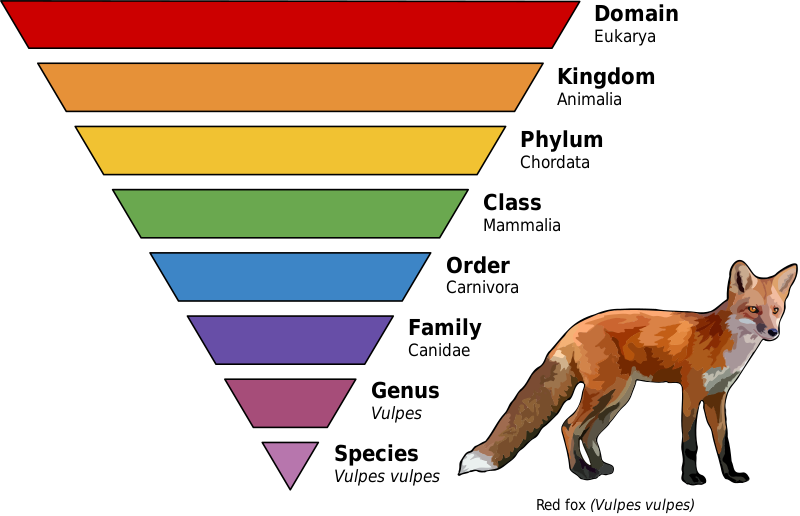
\includegraphics{assets/images/chapters/taxonomic-profiling/800px-Taxonomic_Rank_Graph.svg.png}

\hypertarget{bringing-together-ancient-and-modern-data}{%
\subsection{6. Bringing together ancient and modern
data}\label{bringing-together-ancient-and-modern-data}}

This is the moment where we will the
\href{https://pandas.pydata.org}{Pandas}
\href{https://www.python.org/}{Python} library to perform some data
manipulation.\\
We will also use the \href{https://github.com/apcamargo/taxopy}{Taxopy}
library to work to taxonomic informations.

\begin{Shaded}
\begin{Highlighting}[]
\OperatorTok{!}\NormalTok{ pip install taxopy}
\end{Highlighting}
\end{Shaded}

\begin{verbatim}
Requirement already satisfied: taxopy in /Users/maxime/mambaforge/envs/summer_school_microbiome/lib/python3.9/site-packages (0.10.0)
\end{verbatim}

\begin{Shaded}
\begin{Highlighting}[]
\ImportTok{import}\NormalTok{ pandas }\ImportTok{as}\NormalTok{ pd}
\ImportTok{import}\NormalTok{ taxopy}
\ImportTok{import}\NormalTok{ pickle}
\ImportTok{import}\NormalTok{ gzip}
\end{Highlighting}
\end{Shaded}

\begin{Shaded}
\begin{Highlighting}[]
\ControlFlowTok{with}\NormalTok{ gzip.}\BuiltInTok{open}\NormalTok{(}\StringTok{"../data/taxopy/taxdb.p.gz"}\NormalTok{, }\StringTok{\textquotesingle{}rb\textquotesingle{}}\NormalTok{) }\ImportTok{as}\NormalTok{ tdb:}
\NormalTok{    taxo\_db }\OperatorTok{=}\NormalTok{ pickle.load(tdb)}
\end{Highlighting}
\end{Shaded}

\begin{Shaded}
\begin{Highlighting}[]
\OperatorTok{!}\NormalTok{ head ..}\OperatorTok{/}\NormalTok{results}\OperatorTok{/}\NormalTok{metaphlan}\OperatorTok{/}\NormalTok{ERR5766177.metaphlan\_profile.txt}
\end{Highlighting}
\end{Shaded}

\begin{verbatim}
#mpa_v30_CHOCOPhlAn_201901
#/home/maxime_borry/.conda/envs/maxime/envs/summer_school_microbiome/bin/metaphlan ../results/fastp/ERR5766177.merged.fastq.gz
--input_type fastq --bowtie2out ../results/metaphlan/ERR5766177.bt2.out --nproc 8
#SampleID   Metaphlan_Analysis
#clade_name NCBI_tax_id relative_abundance  additional_species
k__Bacteria 2   82.23198
k__Archaea  2157    17.76802
k__Bacteria|p__Firmicutes   2|1239  33.47957
k__Bacteria|p__Bacteroidetes    2|976   28.4209
k__Bacteria|p__Actinobacteria   2|201174    20.33151
k__Archaea|p__Euryarchaeota 2157|28890  17.76802
\end{verbatim}

\begin{Shaded}
\begin{Highlighting}[]
\NormalTok{ancient\_data }\OperatorTok{=}\NormalTok{ pd.read\_csv(}\StringTok{"../results/metaphlan/ERR5766177.metaphlan\_profile.txt"}\NormalTok{,}
\NormalTok{                            comment}\OperatorTok{=}\StringTok{"\#"}\NormalTok{,}
\NormalTok{                            delimiter}\OperatorTok{=}\StringTok{"}\CharTok{\textbackslash{}t}\StringTok{"}\NormalTok{,}
\NormalTok{                            names}\OperatorTok{=}\NormalTok{[}\StringTok{\textquotesingle{}clade\_name\textquotesingle{}}\NormalTok{,}\StringTok{\textquotesingle{}NCBI\_tax\_id\textquotesingle{}}\NormalTok{,}\StringTok{\textquotesingle{}relative\_abundance\textquotesingle{}}\NormalTok{,}\StringTok{\textquotesingle{}additional\_species\textquotesingle{}}\NormalTok{])}
\end{Highlighting}
\end{Shaded}

\begin{Shaded}
\begin{Highlighting}[]
\NormalTok{ancient\_data.head()}
\end{Highlighting}
\end{Shaded}

clade\_name

NCBI\_tax\_id

relative\_abundance

additional\_species

0

k\_\_Bacteria

2

82.23198

NaN

1

k\_\_Archaea

2157

17.76802

NaN

2

k\_\_Bacteria\textbar p\_\_Firmicutes

2\textbar1239

33.47957

NaN

3

k\_\_Bacteria\textbar p\_\_Bacteroidetes

2\textbar976

28.42090

NaN

4

k\_\_Bacteria\textbar p\_\_Actinobacteria

2\textbar201174

20.33151

NaN

\begin{Shaded}
\begin{Highlighting}[]
\NormalTok{ancient\_data.sample(}\DecValTok{10}\NormalTok{)}
\end{Highlighting}
\end{Shaded}

clade\_name

NCBI\_tax\_id

relative\_abundance

additional\_species

1

k\_\_Archaea

2157

17.76802

NaN

46

k\_\_Bacteria\textbar p\_\_Bacteroidetes\textbar c\_\emph{Bacteroidia\textbar o}\ldots{}

2\textbar976\textbar200643\textbar171549\textbar171552\textbar838\textbar165179

25.75544

k\_\_Bacteria\textbar p\_\_Bacteroidetes\textbar c\_\emph{Bacteroidia\textbar o}\ldots{}

55

k\_\_Bacteria\textbar p\_\_Firmicutes\textbar c\_\_Clostridia\textbar o\_\_Clo\ldots{}

2\textbar1239\textbar186801\textbar186802\textbar186803\textbar189330\textbar88431

0.91178

NaN

18

k\_\_Archaea\textbar p\_\_Euryarchaeota\textbar c\_\emph{Halobacteria\textbar o}\ldots{}

2157\textbar28890\textbar183963\textbar2235

0.71177

NaN

36

k\_\_Bacteria\textbar p\_\_Actinobacteria\textbar c\_\_Actinobacteri\ldots{}

2\textbar201174\textbar1760\textbar85004\textbar31953\textbar1678

9.39377

NaN

65

k\_\_Bacteria\textbar p\_\_Actinobacteria\textbar c\_\_Actinobacteri\ldots{}

2\textbar201174\textbar1760\textbar85004\textbar31953\textbar1678\textbar216816

0.05447

k\_\_Bacteria\textbar p\_\_Actinobacteria\textbar c\_\_Actinobacteri\ldots{}

37

k\_\_Bacteria\textbar p\_\_Firmicutes\textbar c\_\_Clostridia\textbar o\_\_Clo\ldots{}

2\textbar1239\textbar186801\textbar186802\textbar186803\textbar{}

2.16125

NaN

38

k\_\_Bacteria\textbar p\_\_Firmicutes\textbar c\_\_Clostridia\textbar o\_\_Clo\ldots{}

2\textbar1239\textbar186801\textbar186802\textbar541000\textbar216851

1.24537

NaN

26

k\_\_Bacteria\textbar p\_\_Actinobacteria\textbar c\_\_Actinobacteri\ldots{}

2\textbar201174\textbar1760\textbar85004\textbar31953

9.39377

NaN

48

k\_\_Bacteria\textbar p\_\_Firmicutes\textbar c\_\_Clostridia\textbar o\_\_Clo\ldots{}

2\textbar1239\textbar186801\textbar186802\textbar541000\textbar1263\textbar40518

14.96816

k\_\_Bacteria\textbar p\_\_Firmicutes\textbar c\_\_Clostridia\textbar o\_\_Clo\ldots{}

Because for this analysis, we're only going to look at the relative
abundance, we'll only this column, an the
\href{https://www.ncbi.nlm.nih.gov/taxonomy}{TAXID} information

\begin{Shaded}
\begin{Highlighting}[]
\NormalTok{ancient\_data }\OperatorTok{=}\NormalTok{ (}
\NormalTok{    ancient\_data}
\NormalTok{    .rename(columns}\OperatorTok{=}\NormalTok{\{}\StringTok{\textquotesingle{}NCBI\_tax\_id\textquotesingle{}}\NormalTok{: }\StringTok{\textquotesingle{}TAXID\textquotesingle{}}\NormalTok{\})}
\NormalTok{    .drop([}\StringTok{\textquotesingle{}clade\_name\textquotesingle{}}\NormalTok{,}\StringTok{\textquotesingle{}additional\_species\textquotesingle{}}\NormalTok{], axis}\OperatorTok{=}\DecValTok{1}\NormalTok{)}
\NormalTok{)}
\end{Highlighting}
\end{Shaded}

Always investigate your data at first !

\begin{Shaded}
\begin{Highlighting}[]
\NormalTok{ancient\_data.relative\_abundance.}\BuiltInTok{sum}\NormalTok{()}
\end{Highlighting}
\end{Shaded}

\begin{verbatim}
700.00007
\end{verbatim}

\textbf{Pause and think}: A relative abundance of 700\%, really ?

Let's proceed further and try to understand what's happening.

\begin{Shaded}
\begin{Highlighting}[]
\NormalTok{ancient\_data.head()}
\end{Highlighting}
\end{Shaded}

TAXID

relative\_abundance

0

2

82.23198

1

2157

17.76802

2

2\textbar1239

33.47957

3

2\textbar976

28.42090

4

2\textbar201174

20.33151

To make sense of the TAXID, we will use taxopy to get all the taxonomic
related informations such as:

\begin{itemize}
\tightlist
\item
  name of the taxon
\item
  rank of the taxon
\item
  lineage of the taxon
\end{itemize}

\begin{Shaded}
\begin{Highlighting}[]
\CommentTok{\#\#\#\# This function is here to help us get the taxon information}
\CommentTok{\#\#\#\# from the metaphlan taxonomic ID lineage, of the following form}
\CommentTok{\#\#\#\# 2|976|200643|171549|171552|838|165179}

\KeywordTok{def}\NormalTok{ to\_taxopy(taxid\_entry, taxo\_db):}
    \CommentTok{"""Returns a taxopy taxon object}
\CommentTok{    Args:}
\CommentTok{        taxid\_entry(str): metaphlan TAXID taxonomic lineage}
\CommentTok{        taxo\_db(taxopy database)}
\CommentTok{    Returns:}
\CommentTok{        (bool): Returns a taxopy taxon object}
\CommentTok{    """}
\NormalTok{    taxid }\OperatorTok{=}\NormalTok{ taxid\_entry.split(}\StringTok{"|"}\NormalTok{)[}\OperatorTok{{-}}\DecValTok{1}\NormalTok{] }\CommentTok{\# get the last element}
    \ControlFlowTok{try}\NormalTok{:}
        \ControlFlowTok{if} \BuiltInTok{len}\NormalTok{(taxid) }\OperatorTok{\textgreater{}} \DecValTok{0}\NormalTok{:}
            \ControlFlowTok{return}\NormalTok{ taxopy.Taxon(}\BuiltInTok{int}\NormalTok{(taxid), taxo\_db) }\CommentTok{\# if it\textquotesingle{}s not empty, get the taxon corresponding to the taxid}
        \ControlFlowTok{else}\NormalTok{:}
            \ControlFlowTok{return}\NormalTok{ taxopy.Taxon(}\DecValTok{12908}\NormalTok{, taxo\_db) }\CommentTok{\# otherwise, return the taxon associated with unclassified sequences}
    \ControlFlowTok{except}\NormalTok{ taxopy.exceptions.TaxidError }\ImportTok{as}\NormalTok{ e:}
        \ControlFlowTok{return}\NormalTok{ taxopy.Taxon(}\DecValTok{12908}\NormalTok{, taxo\_db)}
\end{Highlighting}
\end{Shaded}

\begin{Shaded}
\begin{Highlighting}[]
\NormalTok{ancient\_data[}\StringTok{\textquotesingle{}taxopy\textquotesingle{}}\NormalTok{] }\OperatorTok{=}\NormalTok{ ancient\_data[}\StringTok{\textquotesingle{}TAXID\textquotesingle{}}\NormalTok{].}\BuiltInTok{apply}\NormalTok{(to\_taxopy, taxo\_db}\OperatorTok{=}\NormalTok{taxo\_db)}
\end{Highlighting}
\end{Shaded}

\begin{Shaded}
\begin{Highlighting}[]
\NormalTok{ancient\_data.head()}
\end{Highlighting}
\end{Shaded}

TAXID

relative\_abundance

taxopy

0

2

82.23198

s\_\_Bacteria

1

2157

17.76802

s\_\_Archaea

2

2\textbar1239

33.47957

s\_\_Bacteria;c\_\_Terrabacteria group;p\_\_Firmicutes

3

2\textbar976

28.42090

s\_\_Bacteria;c\_\_FCB group;p\_\_Bacteroidetes

4

2\textbar201174

20.33151

s\_\_Bacteria;c\_\_Terrabacteria group;p\_\_Actinoba\ldots{}

\begin{Shaded}
\begin{Highlighting}[]
\NormalTok{ancient\_data }\OperatorTok{=}\NormalTok{ ancient\_data.assign(}
\NormalTok{    rank }\OperatorTok{=}\NormalTok{ ancient\_data.taxopy.}\BuiltInTok{apply}\NormalTok{(}\KeywordTok{lambda}\NormalTok{ x: x.rank),}
\NormalTok{    name }\OperatorTok{=}\NormalTok{ ancient\_data.taxopy.}\BuiltInTok{apply}\NormalTok{(}\KeywordTok{lambda}\NormalTok{ x: x.name),}
\NormalTok{    lineage }\OperatorTok{=}\NormalTok{ ancient\_data.taxopy.}\BuiltInTok{apply}\NormalTok{(}\KeywordTok{lambda}\NormalTok{ x: x.name\_lineage),}
\NormalTok{)}
\end{Highlighting}
\end{Shaded}

\begin{Shaded}
\begin{Highlighting}[]
\NormalTok{ancient\_data}
\end{Highlighting}
\end{Shaded}

TAXID

relative\_abundance

taxopy

rank

name

lineage

0

2

82.23198

s\_\_Bacteria

superkingdom

Bacteria

{[}Bacteria, cellular organisms, root{]}

1

2157

17.76802

s\_\_Archaea

superkingdom

Archaea

{[}Archaea, cellular organisms, root{]}

2

2\textbar1239

33.47957

s\_\_Bacteria;c\_\_Terrabacteria group;p\_\_Firmicutes

phylum

Firmicutes

{[}Firmicutes, Terrabacteria group, Bacteria, ce\ldots{}

3

2\textbar976

28.42090

s\_\_Bacteria;c\_\_FCB group;p\_\_Bacteroidetes

phylum

Bacteroidetes

{[}Bacteroidetes, Bacteroidetes/Chlorobi group, \ldots{}

4

2\textbar201174

20.33151

s\_\_Bacteria;c\_\_Terrabacteria group;p\_\_Actinoba\ldots{}

phylum

Actinobacteria

{[}Actinobacteria, Terrabacteria group, Bacteria\ldots{}

\ldots{}

\ldots{}

\ldots{}

\ldots{}

\ldots{}

\ldots{}

\ldots{}

62

2\textbar1239\textbar186801\textbar186802\textbar186803\textbar572511\textbar33039

0.24910

s\_\_Bacteria;c\_\_Terrabacteria group;p\_\_Firmicut\ldots{}

species

{[}Ruminococcus{]} torques

{[}{[}Ruminococcus{]} torques, Mediterraneibacter, L\ldots{}

63

2\textbar201174\textbar84998\textbar84999\textbar84107\textbar1472762\textbar1232426

0.17084

s\_\_Bacteria;c\_\_Terrabacteria group;p\_\_Actinoba\ldots{}

species

{[}Collinsella{]} massiliensis

{[}{[}Collinsella{]} massiliensis, Enorma, Coriobact\ldots{}

64

2\textbar1239\textbar186801\textbar186802\textbar186803\textbar189330\textbar39486

0.07690

s\_\_Bacteria;c\_\_Terrabacteria group;p\_\_Firmicut\ldots{}

species

Dorea formicigenerans

{[}Dorea formicigenerans, Dorea, Lachnospiraceae\ldots{}

65

2\textbar201174\textbar1760\textbar85004\textbar31953\textbar1678\textbar216816

0.05447

s\_\_Bacteria;c\_\_Terrabacteria group;p\_\_Actinoba\ldots{}

species

Bifidobacterium longum

{[}Bifidobacterium longum, Bifidobacterium, Bifi\ldots{}

66

2\textbar1239\textbar186801\textbar186802\textbar541000\textbar1263\textbar1262959

0.01440

s\_\_Bacteria;c\_\_Terrabacteria group;p\_\_Firmicut\ldots{}

species

Ruminococcus sp. CAG:488

{[}Ruminococcus sp. CAG:488, environmental sampl\ldots{}

67 rows × 6 columns

Because our modern data are split by ranks, we'll first split our
ancient sample by rank

Which of the entries are at the \texttt{species\ rank} level ?

\begin{Shaded}
\begin{Highlighting}[]
\NormalTok{ancient\_species }\OperatorTok{=}\NormalTok{ ancient\_data.query(}\StringTok{"rank == \textquotesingle{}species\textquotesingle{}"}\NormalTok{)}
\end{Highlighting}
\end{Shaded}

\begin{Shaded}
\begin{Highlighting}[]
\NormalTok{ancient\_species.head()}
\end{Highlighting}
\end{Shaded}

TAXID

relative\_abundance

taxopy

rank

name

lineage

46

2\textbar976\textbar200643\textbar171549\textbar171552\textbar838\textbar165179

25.75544

s\_\_Bacteria;c\_\_FCB group;p\_\_Bacteroidetes;c\_\_B\ldots{}

species

Prevotella copri

{[}Prevotella copri, Prevotella, Prevotellaceae,\ldots{}

47

2157\textbar28890\textbar183925\textbar2158\textbar2159\textbar2172\textbar2173

17.05626

s\_\_Archaea;p\_\_Euryarchaeota;c\_\_Methanomada gro\ldots{}

species

Methanobrevibacter smithii

{[}Methanobrevibacter smithii, Methanobrevibacte\ldots{}

48

2\textbar1239\textbar186801\textbar186802\textbar541000\textbar1263\textbar40518

14.96816

s\_\_Bacteria;c\_\_Terrabacteria group;p\_\_Firmicut\ldots{}

species

Ruminococcus bromii

{[}Ruminococcus bromii, Ruminococcus, Oscillospi\ldots{}

49

2\textbar1239\textbar186801\textbar186802\textbar186803\textbar841\textbar301302

13.57908

s\_\_Bacteria;c\_\_Terrabacteria group;p\_\_Firmicut\ldots{}

species

Roseburia faecis

{[}Roseburia faecis, Roseburia, Lachnospiraceae,\ldots{}

50

2\textbar201174\textbar84998\textbar84999\textbar84107\textbar102106\textbar74426

9.49165

s\_\_Bacteria;c\_\_Terrabacteria group;p\_\_Actinoba\ldots{}

species

Collinsella aerofaciens

{[}Collinsella aerofaciens, Collinsella, Corioba\ldots{}

Let's do a bit of renaming to prepare for what's coming next

\begin{Shaded}
\begin{Highlighting}[]
\NormalTok{ancient\_species }\OperatorTok{=}\NormalTok{ ancient\_species[[}\StringTok{\textquotesingle{}relative\_abundance\textquotesingle{}}\NormalTok{,}\StringTok{\textquotesingle{}name\textquotesingle{}}\NormalTok{]].set\_index(}\StringTok{\textquotesingle{}name\textquotesingle{}}\NormalTok{).rename(columns}\OperatorTok{=}\NormalTok{\{}\StringTok{\textquotesingle{}relative\_abundance\textquotesingle{}}\NormalTok{:}\StringTok{\textquotesingle{}ERR5766177\textquotesingle{}}\NormalTok{\})}
\end{Highlighting}
\end{Shaded}

\begin{Shaded}
\begin{Highlighting}[]
\NormalTok{ancient\_species.head()}
\end{Highlighting}
\end{Shaded}

ERR5766177

name

Prevotella copri

25.75544

Methanobrevibacter smithii

17.05626

Ruminococcus bromii

14.96816

Roseburia faecis

13.57908

Collinsella aerofaciens

9.49165

\begin{Shaded}
\begin{Highlighting}[]
\NormalTok{ancient\_phylums }\OperatorTok{=}\NormalTok{ ancient\_data.query(}\StringTok{"rank == \textquotesingle{}phylum\textquotesingle{}"}\NormalTok{)}
\end{Highlighting}
\end{Shaded}

\begin{Shaded}
\begin{Highlighting}[]
\NormalTok{ancient\_phylums }\OperatorTok{=}\NormalTok{ ancient\_phylums[[}\StringTok{\textquotesingle{}relative\_abundance\textquotesingle{}}\NormalTok{,}\StringTok{\textquotesingle{}name\textquotesingle{}}\NormalTok{]].set\_index(}\StringTok{\textquotesingle{}name\textquotesingle{}}\NormalTok{).rename(columns}\OperatorTok{=}\NormalTok{\{}\StringTok{\textquotesingle{}relative\_abundance\textquotesingle{}}\NormalTok{:}\StringTok{\textquotesingle{}ERR5766177\textquotesingle{}}\NormalTok{\})}
\end{Highlighting}
\end{Shaded}

\begin{Shaded}
\begin{Highlighting}[]
\NormalTok{ancient\_phylums}
\end{Highlighting}
\end{Shaded}

ERR5766177

name

Firmicutes

33.47957

Bacteroidetes

28.42090

Actinobacteria

20.33151

Euryarchaeota

17.76802

Now, let's go back to the 700\% relative abundance issue\ldots{}

\begin{Shaded}
\begin{Highlighting}[]
\NormalTok{ancient\_data.groupby(}\StringTok{\textquotesingle{}rank\textquotesingle{}}\NormalTok{)[}\StringTok{\textquotesingle{}relative\_abundance\textquotesingle{}}\NormalTok{].}\BuiltInTok{sum}\NormalTok{()}
\end{Highlighting}
\end{Shaded}

\begin{verbatim}
rank
class            99.72648
family           83.49854
genus            97.56524
no rank          19.48331
order            99.72648
phylum          100.00000
species         100.00002
superkingdom    100.00000
Name: relative_abundance, dtype: float64
\end{verbatim}

Seems better, right ?

\textbf{Pause and think: why don't we get exactly 100\%} ?

Now let's load our modern reference samples

\begin{Shaded}
\begin{Highlighting}[]
\NormalTok{modern\_phylums }\OperatorTok{=}\NormalTok{ pd.read\_csv(}\StringTok{"../data/curated\_metagenomics/modern\_sources\_phylum.csv"}\NormalTok{, index\_col}\OperatorTok{=}\DecValTok{0}\NormalTok{)}
\NormalTok{modern\_phylums.head()}
\end{Highlighting}
\end{Shaded}

de028ad4-7ae6-11e9-a106-68b59976a384

PNP\_Main\_283

PNP\_Validation\_55

G80275

PNP\_Main\_363

SAMEA7045572

SAMEA7045355

HD-13

EGAR00001420773\_9002000001423910

SID5428-4

\ldots{}

A46\_02\_1FE

TZ\_87532

A94\_01\_1FE

KHG\_7

LDK\_4

KHG\_9

A48\_01\_1FE

KHG\_1

TZ\_81781

A09\_01\_1FE

Bacteroidetes

0.00000

17.44332

82.86400

69.99087

31.93081

51.76204

53.32801

74.59667

8.81074

26.39694

\ldots{}

1.97760

1.49601

67.21410

4.29848

68.16890

38.59709

14.81828

10.13908

57.14031

11.61544

Firmicutes

95.24231

60.47031

16.53946

22.81977

65.23075

41.96928

45.77661

23.51065

54.35341

62.23094

\ldots{}

76.68499

78.13269

29.72394

33.51772

19.11149

46.87139

72.68136

35.43789

40.57101

24.72113

Proteobacteria

4.49959

0.77098

0.05697

4.07757

0.27316

3.33972

0.02001

1.72865

0.00000

1.81016

\ldots{}

16.57250

0.76159

2.35058

9.83772

5.32392

0.19699

3.64655

17.64151

0.30580

56.20177

Actinobacteria

0.25809

10.27631

0.45187

1.11902

2.31075

2.92715

0.77667

0.16403

36.55138

1.19951

\ldots{}

3.01814

19.20468

0.69913

46.99479

7.39093

14.26365

5.47750

36.77145

1.16426

7.40894

Verrucomicrobia

0.00000

0.00784

0.00000

1.99276

0.25451

0.00000

0.00000

0.00000

0.09940

3.29795

\ldots{}

0.05011

0.00000

0.00000

0.00000

0.00000

0.00000

0.00000

0.00000

0.00000

0.00000

5 rows × 200 columns

\begin{Shaded}
\begin{Highlighting}[]
\NormalTok{modern\_species }\OperatorTok{=}\NormalTok{ pd.read\_csv(}\StringTok{"../data/curated\_metagenomics/modern\_sources\_species.csv"}\NormalTok{, index\_col}\OperatorTok{=}\DecValTok{0}\NormalTok{)}
\end{Highlighting}
\end{Shaded}

\begin{Shaded}
\begin{Highlighting}[]
\NormalTok{modern\_species.head()}
\end{Highlighting}
\end{Shaded}

de028ad4-7ae6-11e9-a106-68b59976a384

PNP\_Main\_283

PNP\_Validation\_55

G80275

PNP\_Main\_363

SAMEA7045572

SAMEA7045355

HD-13

EGAR00001420773\_9002000001423910

SID5428-4

\ldots{}

A46\_02\_1FE

TZ\_87532

A94\_01\_1FE

KHG\_7

LDK\_4

KHG\_9

A48\_01\_1FE

KHG\_1

TZ\_81781

A09\_01\_1FE

Bacteroides vulgatus

0.0

0.60446

1.59911

4.39085

0.04494

4.66505

2.99431

29.30325

1.48560

0.98818

\ldots{}

0.20717

0.0

0.00309

0.48891

0.00000

0.02230

0.00000

0.15112

0.0

0.00836

Bacteroides stercoris

0.0

0.00546

0.00000

0.00000

2.50789

0.00000

20.57498

8.28443

1.23261

0.00000

\ldots{}

0.00000

0.0

0.00000

0.00693

0.00000

0.02603

0.00000

0.19318

0.0

0.00000

Acidaminococcus intestini

0.0

0.00000

0.00000

0.00000

0.00000

0.00000

0.00000

0.00000

0.32822

0.00000

\ldots{}

0.00000

0.0

0.00000

0.00000

0.00000

0.00000

0.00000

0.00000

0.0

0.00000

Eubacterium sp CAG 38

0.0

0.06712

0.81149

0.05247

0.26027

0.00000

0.00000

2.62415

0.46585

0.23372

\ldots{}

0.78140

0.0

0.00000

0.00499

0.00000

0.02446

0.00000

0.00000

0.0

0.00000

Parabacteroides distasonis

0.0

1.34931

2.00672

5.85067

0.59019

7.00027

1.28075

0.61758

0.07383

2.80355

\ldots{}

0.11423

0.0

0.01181

0.01386

0.03111

0.07463

0.15597

0.07541

0.0

0.01932

5 rows × 200 columns

Now, let's merge our ancient sample with the modern data in one single
table

\begin{Shaded}
\begin{Highlighting}[]
\NormalTok{all\_species }\OperatorTok{=}\NormalTok{ ancient\_species.merge(modern\_species, left\_index}\OperatorTok{=}\VariableTok{True}\NormalTok{, right\_index}\OperatorTok{=}\VariableTok{True}\NormalTok{, how}\OperatorTok{=}\StringTok{\textquotesingle{}outer\textquotesingle{}}\NormalTok{).fillna(}\DecValTok{0}\NormalTok{)}
\NormalTok{all\_phylums }\OperatorTok{=}\NormalTok{ ancient\_phylums.merge(modern\_phylums, left\_index}\OperatorTok{=}\VariableTok{True}\NormalTok{, right\_index}\OperatorTok{=}\VariableTok{True}\NormalTok{, how}\OperatorTok{=}\StringTok{\textquotesingle{}outer\textquotesingle{}}\NormalTok{).fillna(}\DecValTok{0}\NormalTok{)}
\end{Highlighting}
\end{Shaded}

Finally, let's load the metadata

\begin{Shaded}
\begin{Highlighting}[]
\NormalTok{metadata }\OperatorTok{=}\NormalTok{ pd.read\_csv(}\StringTok{"../data/metadata/curated\_metagenomics\_modern\_sources.csv"}\NormalTok{)}
\end{Highlighting}
\end{Shaded}

\begin{Shaded}
\begin{Highlighting}[]
\NormalTok{metadata.head()}
\end{Highlighting}
\end{Shaded}

study\_name

sample\_id

subject\_id

body\_site

antibiotics\_current\_use

study\_condition

disease

age

infant\_age

age\_category

\ldots{}

hla\_drb11

birth\_order

age\_twins\_started\_to\_live\_apart

zigosity

brinkman\_index

alcohol\_numeric

breastfeeding\_duration

formula\_first\_day

ALT

eGFR

0

ShaoY\_2019

de028ad4-7ae6-11e9-a106-68b59976a384

C01528\_ba

stool

no

control

healthy

0.0

4.0

newborn

\ldots{}

NaN

NaN

NaN

NaN

NaN

NaN

NaN

NaN

NaN

NaN

1

ZeeviD\_2015

PNP\_Main\_283

PNP\_Main\_283

stool

no

control

healthy

NaN

NaN

adult

\ldots{}

NaN

NaN

NaN

NaN

NaN

NaN

NaN

NaN

NaN

NaN

2

ZeeviD\_2015

PNP\_Validation\_55

PNP\_Validation\_55

stool

no

control

healthy

NaN

NaN

adult

\ldots{}

NaN

NaN

NaN

NaN

NaN

NaN

NaN

NaN

NaN

NaN

3

VatanenT\_2016

G80275

T014806

stool

no

control

healthy

1.0

NaN

child

\ldots{}

NaN

NaN

NaN

NaN

NaN

NaN

NaN

NaN

NaN

NaN

4

ZeeviD\_2015

PNP\_Main\_363

PNP\_Main\_363

stool

no

control

healthy

NaN

NaN

adult

\ldots{}

NaN

NaN

NaN

NaN

NaN

NaN

NaN

NaN

NaN

NaN

5 rows × 130 columns

\hypertarget{comparing-ancient-and-modern-samples}{%
\subsection{7. Comparing ancient and modern
samples}\label{comparing-ancient-and-modern-samples}}

\hypertarget{taxonomic-composition}{%
\subsubsection{7.1 Taxonomic composition}\label{taxonomic-composition}}

One common plot in microbiome papers in a stacked barplot, often at the
phylum or family level.

First, we'll do some renaming, to make the value of the metadata
variables a bit easier to understand

\begin{Shaded}
\begin{Highlighting}[]
\NormalTok{group\_info }\OperatorTok{=}\NormalTok{ (}
\NormalTok{    metadata[}\StringTok{\textquotesingle{}non\_westernized\textquotesingle{}}\NormalTok{]}
\NormalTok{    .}\BuiltInTok{map}\NormalTok{(\{}\StringTok{\textquotesingle{}no\textquotesingle{}}\NormalTok{:}\StringTok{\textquotesingle{}westernized\textquotesingle{}}\NormalTok{,}\StringTok{\textquotesingle{}yes\textquotesingle{}}\NormalTok{:}\StringTok{\textquotesingle{}non\_westernized\textquotesingle{}}\NormalTok{\}) }\CommentTok{\# for the non\_westernized in the modern sample metadata, rename the value levels}
\NormalTok{    .to\_frame(name}\OperatorTok{=}\StringTok{\textquotesingle{}group\textquotesingle{}}\NormalTok{).set\_index(metadata[}\StringTok{\textquotesingle{}sample\_id\textquotesingle{}}\NormalTok{]) }\CommentTok{\# rename the column to group}
\NormalTok{    .reset\_index()}
\NormalTok{    .append(\{}\StringTok{\textquotesingle{}sample\_id\textquotesingle{}}\NormalTok{:}\StringTok{\textquotesingle{}ERR5766177\textquotesingle{}}\NormalTok{, }\StringTok{\textquotesingle{}group\textquotesingle{}}\NormalTok{:}\StringTok{\textquotesingle{}ancient\textquotesingle{}}\NormalTok{\}, ignore\_index}\OperatorTok{=}\VariableTok{True}\NormalTok{) }\CommentTok{\# add the ancient sample}
\NormalTok{)}
\NormalTok{group\_info}
\end{Highlighting}
\end{Shaded}

\begin{verbatim}
/var/folders/1c/l1qb09f15jddsh65f6xv1n_r0000gp/T/ipykernel_40830/27419655.py:2:
FutureWarning: The frame.append method is deprecated and will be removed from pandas in a future version.
Use pandas.concat instead.
  metadata['non_westernized']
\end{verbatim}

sample\_id

group

0

de028ad4-7ae6-11e9-a106-68b59976a384

westernized

1

PNP\_Main\_283

westernized

2

PNP\_Validation\_55

westernized

3

G80275

westernized

4

PNP\_Main\_363

westernized

\ldots{}

\ldots{}

\ldots{}

196

A48\_01\_1FE

non\_westernized

197

KHG\_1

non\_westernized

198

TZ\_81781

non\_westernized

199

A09\_01\_1FE

non\_westernized

200

ERR5766177

ancient

201 rows × 2 columns

We need transform our data in
\href{https://cran.r-project.org/web/packages/tidyr/vignettes/tidy-data.html}{tidy}
format to plot with
\href{https://plotnine.readthedocs.io/en/stable/}{plotnine}, a python
clone of \href{https://ggplot2.tidyverse.org/index.html}{ggplot}.\\
We then add the group information (Westernized, non westernized, or
ancient sample), and compute the mean abundance for each phylum.

First we transpose the dataframe to have the samples as index, and the
phylums as columns

We then add the metadata information

\begin{Shaded}
\begin{Highlighting}[]
\NormalTok{(}
\NormalTok{    all\_phylums}
\NormalTok{    .transpose()}
\NormalTok{    .merge(group\_info, left\_index}\OperatorTok{=}\VariableTok{True}\NormalTok{, right\_on}\OperatorTok{=}\StringTok{\textquotesingle{}sample\_id\textquotesingle{}}\NormalTok{)}
\NormalTok{)}
\end{Highlighting}
\end{Shaded}

Actinobacteria

Apicomplexa

Ascomycota

Bacteroidetes

Basidiomycota

Candidatus Melainabacteria

Chlamydiae

Chloroflexi

Cyanobacteria

Deferribacteres

\ldots{}

Fusobacteria

Lentisphaerae

Planctomycetes

Proteobacteria

Spirochaetes

Synergistetes

Tenericutes

Verrucomicrobia

sample\_id

group

200

20.33151

0.0

0.0

28.42090

0.0

0.0

0.0

0.0

0.0

0.0

\ldots{}

0.0

0.00000

0.0

0.00000

0.00000

0.0

0.0

0.00000

ERR5766177

ancient

0

0.25809

0.0

0.0

0.00000

0.0

0.0

0.0

0.0

0.0

0.0

\ldots{}

0.0

0.00000

0.0

4.49959

0.00000

0.0

0.0

0.00000

de028ad4-7ae6-11e9-a106-68b59976a384

westernized

1

10.27631

0.0

0.0

17.44332

0.0

0.0

0.0

0.0

0.0

0.0

\ldots{}

0.0

0.01486

0.0

0.77098

0.00000

0.0

0.0

0.00784

PNP\_Main\_283

westernized

2

0.45187

0.0

0.0

82.86400

0.0

0.0

0.0

0.0

0.0

0.0

\ldots{}

0.0

0.00000

0.0

0.05697

0.00000

0.0

0.0

0.00000

PNP\_Validation\_55

westernized

3

1.11902

0.0

0.0

69.99087

0.0

0.0

0.0

0.0

0.0

0.0

\ldots{}

0.0

0.00000

0.0

4.07757

0.00000

0.0

0.0

1.99276

G80275

westernized

\ldots{}

\ldots{}

\ldots{}

\ldots{}

\ldots{}

\ldots{}

\ldots{}

\ldots{}

\ldots{}

\ldots{}

\ldots{}

\ldots{}

\ldots{}

\ldots{}

\ldots{}

\ldots{}

\ldots{}

\ldots{}

\ldots{}

\ldots{}

\ldots{}

\ldots{}

195

14.26365

0.0

0.0

38.59709

0.0

0.0

0.0

0.0

0.0

0.0

\ldots{}

0.0

0.00000

0.0

0.19699

0.00000

0.0

0.0

0.00000

KHG\_9

non\_westernized

196

5.47750

0.0

0.0

14.81828

0.0

0.0

0.0

0.0

0.0

0.0

\ldots{}

0.0

0.00000

0.0

3.64655

0.09964

0.0

0.0

0.00000

A48\_01\_1FE

non\_westernized

197

36.77145

0.0

0.0

10.13908

0.0

0.0

0.0

0.0

0.0

0.0

\ldots{}

0.0

0.00000

0.0

17.64151

0.00000

0.0

0.0

0.00000

KHG\_1

non\_westernized

198

1.16426

0.0

0.0

57.14031

0.0

0.0

0.0

0.0

0.0

0.0

\ldots{}

0.0

0.00000

0.0

0.30580

0.70467

0.0

0.0

0.00000

TZ\_81781

non\_westernized

199

7.40894

0.0

0.0

11.61544

0.0

0.0

0.0

0.0

0.0

0.0

\ldots{}

0.0

0.00000

0.0

56.20177

0.00000

0.0

0.0

0.00000

A09\_01\_1FE

non\_westernized

201 rows × 24 columns

Now, we need it in the tidy format

\begin{Shaded}
\begin{Highlighting}[]
\NormalTok{tidy\_phylums }\OperatorTok{=}\NormalTok{ (}
\NormalTok{    all\_phylums}
\NormalTok{    .transpose()}
\NormalTok{    .merge(group\_info, left\_index}\OperatorTok{=}\VariableTok{True}\NormalTok{, right\_on}\OperatorTok{=}\StringTok{\textquotesingle{}sample\_id\textquotesingle{}}\NormalTok{)}
\NormalTok{    .melt(id\_vars}\OperatorTok{=}\NormalTok{[}\StringTok{\textquotesingle{}sample\_id\textquotesingle{}}\NormalTok{, }\StringTok{\textquotesingle{}group\textquotesingle{}}\NormalTok{], value\_name}\OperatorTok{=}\StringTok{\textquotesingle{}relative\_abundance\textquotesingle{}}\NormalTok{, var\_name}\OperatorTok{=}\StringTok{\textquotesingle{}Phylum\textquotesingle{}}\NormalTok{, ignore\_index}\OperatorTok{=}\VariableTok{True}\NormalTok{)}
\NormalTok{)}
\end{Highlighting}
\end{Shaded}

Finally, we only want to keep the mean relative abundance for each
phylum

\begin{Shaded}
\begin{Highlighting}[]
\NormalTok{tidy\_phylums }\OperatorTok{=}\NormalTok{ tidy\_phylums.groupby([}\StringTok{\textquotesingle{}group\textquotesingle{}}\NormalTok{, }\StringTok{\textquotesingle{}Phylum\textquotesingle{}}\NormalTok{]).mean().reset\_index()}
\end{Highlighting}
\end{Shaded}

\begin{Shaded}
\begin{Highlighting}[]
\NormalTok{tidy\_phylums.groupby(}\StringTok{\textquotesingle{}group\textquotesingle{}}\NormalTok{)[}\StringTok{\textquotesingle{}relative\_abundance\textquotesingle{}}\NormalTok{].}\BuiltInTok{sum}\NormalTok{()}
\end{Highlighting}
\end{Shaded}

\begin{verbatim}
group
ancient            100.000000
non_westernized     99.710255
westernized         99.905089
Name: relative_abundance, dtype: float64
\end{verbatim}

\begin{Shaded}
\begin{Highlighting}[]
\ImportTok{from}\NormalTok{ plotnine }\ImportTok{import} \OperatorTok{*}
\end{Highlighting}
\end{Shaded}

\begin{Shaded}
\begin{Highlighting}[]
\NormalTok{ggplot(tidy\_phylums, aes(x}\OperatorTok{=}\StringTok{\textquotesingle{}group\textquotesingle{}}\NormalTok{, y}\OperatorTok{=}\StringTok{\textquotesingle{}relative\_abundance\textquotesingle{}}\NormalTok{, fill}\OperatorTok{=}\StringTok{\textquotesingle{}Phylum\textquotesingle{}}\NormalTok{)) }\OperatorTok{\textbackslash{}}
\OperatorTok{+}\NormalTok{ geom\_bar(position}\OperatorTok{=}\StringTok{\textquotesingle{}stack\textquotesingle{}}\NormalTok{, stat}\OperatorTok{=}\StringTok{\textquotesingle{}identity\textquotesingle{}}\NormalTok{) }\OperatorTok{\textbackslash{}}
\OperatorTok{+}\NormalTok{ ylab(}\StringTok{\textquotesingle{}mean abundance\textquotesingle{}}\NormalTok{) }\OperatorTok{\textbackslash{}}
\OperatorTok{+}\NormalTok{ xlab(}\StringTok{""}\NormalTok{) }\OperatorTok{\textbackslash{}}
\OperatorTok{+}\NormalTok{ theme\_classic()}
\end{Highlighting}
\end{Shaded}

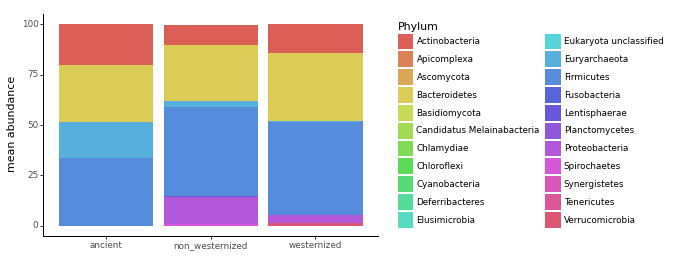
\includegraphics{assets/images/chapters/taxonomic-profiling/analysis_80_0.png}

\begin{verbatim}
<ggplot: (406187548)>
\end{verbatim}

\hypertarget{ecological-diversity}{%
\subsubsection{7.2 Ecological diversity}\label{ecological-diversity}}

\hypertarget{alpha-diversity}{%
\paragraph{7.2.1 Alpha diversity}\label{alpha-diversity}}

Alpha diversity is the measure of diversity withing each sample. It is
used to estimate how many species are present in a sample, and how
diverse they are.\\
We'll use the python library \href{http://scikit-bio.org/}{scikit-bio}
to compute it, and the \href{https://plotnine.readthedocs.io/}{plotnine}
library (a python port of
\href{https://ggplot2.tidyverse.org/reference/ggplot.html}{ggplot2} to
visualize the results).

\begin{Shaded}
\begin{Highlighting}[]
\ImportTok{import}\NormalTok{ skbio}
\end{Highlighting}
\end{Shaded}

Let's compute the
\href{https://en.wikipedia.org/wiki/Species_richness}{species richness},
the
\href{https://www.biologydiscussion.com/biodiversity/types/2-types-of-diversity-indices-of-biodiversity/8388}{Shannon,
and Simpson index of diversity} index

\begin{Shaded}
\begin{Highlighting}[]
\NormalTok{shannon }\OperatorTok{=}\NormalTok{ skbio.diversity.alpha\_diversity(metric}\OperatorTok{=}\StringTok{\textquotesingle{}shannon\textquotesingle{}}\NormalTok{, counts}\OperatorTok{=}\NormalTok{all\_species.transpose(), ids}\OperatorTok{=}\NormalTok{all\_species.columns)}
\NormalTok{simpson }\OperatorTok{=}\NormalTok{ skbio.diversity.alpha\_diversity(metric}\OperatorTok{=}\StringTok{\textquotesingle{}simpson\textquotesingle{}}\NormalTok{, counts}\OperatorTok{=}\NormalTok{all\_species.transpose(), ids}\OperatorTok{=}\NormalTok{all\_species.columns)}
\NormalTok{richness }\OperatorTok{=}\NormalTok{ (all\_species }\OperatorTok{!=} \DecValTok{0}\NormalTok{).astype(}\BuiltInTok{int}\NormalTok{).}\BuiltInTok{sum}\NormalTok{(axis}\OperatorTok{=}\DecValTok{0}\NormalTok{)}
\NormalTok{alpha\_diversity }\OperatorTok{=}\NormalTok{ (shannon.to\_frame(name}\OperatorTok{=}\StringTok{\textquotesingle{}shannon\textquotesingle{}}\NormalTok{)}
\NormalTok{                   .merge(simpson.to\_frame(name}\OperatorTok{=}\StringTok{\textquotesingle{}simpson\textquotesingle{}}\NormalTok{), left\_index}\OperatorTok{=}\VariableTok{True}\NormalTok{, right\_index}\OperatorTok{=}\VariableTok{True}\NormalTok{)}
\NormalTok{                   .merge(richness.to\_frame(name}\OperatorTok{=}\StringTok{\textquotesingle{}richness\textquotesingle{}}\NormalTok{), left\_index}\OperatorTok{=}\VariableTok{True}\NormalTok{, right\_index}\OperatorTok{=}\VariableTok{True}\NormalTok{))}
\NormalTok{alpha\_diversity}
\end{Highlighting}
\end{Shaded}

shannon

simpson

richness

ERR5766177

3.032945

0.844769

21

de028ad4-7ae6-11e9-a106-68b59976a384

0.798112

0.251280

11

PNP\_Main\_283

5.092878

0.954159

118

PNP\_Validation\_55

3.670162

0.812438

72

G80275

3.831358

0.876712

66

\ldots{}

\ldots{}

\ldots{}

\ldots{}

KHG\_9

3.884285

0.861683

87

A48\_01\_1FE

4.377755

0.930024

53

KHG\_1

3.733834

0.875335

108

TZ\_81781

2.881856

0.719491

44

A09\_01\_1FE

2.982322

0.719962

75

201 rows × 3 columns

Let's load the group information from the metadata

\begin{Shaded}
\begin{Highlighting}[]
\NormalTok{alpha\_diversity }\OperatorTok{=}\NormalTok{ (}
\NormalTok{    alpha\_diversity}
\NormalTok{    .merge(metadata[[}\StringTok{\textquotesingle{}sample\_id\textquotesingle{}}\NormalTok{, }\StringTok{\textquotesingle{}non\_westernized\textquotesingle{}}\NormalTok{]], left\_index}\OperatorTok{=}\VariableTok{True}\NormalTok{, right\_on}\OperatorTok{=}\StringTok{\textquotesingle{}sample\_id\textquotesingle{}}\NormalTok{, how}\OperatorTok{=}\StringTok{\textquotesingle{}outer\textquotesingle{}}\NormalTok{)}
\NormalTok{    .set\_index(}\StringTok{\textquotesingle{}sample\_id\textquotesingle{}}\NormalTok{)}
\NormalTok{    .rename(columns}\OperatorTok{=}\NormalTok{\{}\StringTok{\textquotesingle{}non\_westernized\textquotesingle{}}\NormalTok{:}\StringTok{\textquotesingle{}group\textquotesingle{}}\NormalTok{\})}
\NormalTok{)}
\NormalTok{alpha\_diversity[}\StringTok{\textquotesingle{}group\textquotesingle{}}\NormalTok{] }\OperatorTok{=}\NormalTok{ alpha\_diversity[}\StringTok{\textquotesingle{}group\textquotesingle{}}\NormalTok{].replace(\{}\StringTok{\textquotesingle{}yes\textquotesingle{}}\NormalTok{:}\StringTok{\textquotesingle{}non\_westernized\textquotesingle{}}\NormalTok{,}\StringTok{\textquotesingle{}no\textquotesingle{}}\NormalTok{:}\StringTok{\textquotesingle{}westernized\textquotesingle{}}\NormalTok{, pd.NA:}\StringTok{\textquotesingle{}ERR5766177\textquotesingle{}}\NormalTok{\})}
\end{Highlighting}
\end{Shaded}

\begin{Shaded}
\begin{Highlighting}[]
\NormalTok{alpha\_diversity}
\end{Highlighting}
\end{Shaded}

shannon

simpson

richness

group

sample\_id

ERR5766177

3.032945

0.844769

21

ERR5766177

de028ad4-7ae6-11e9-a106-68b59976a384

0.798112

0.251280

11

westernized

PNP\_Main\_283

5.092878

0.954159

118

westernized

PNP\_Validation\_55

3.670162

0.812438

72

westernized

G80275

3.831358

0.876712

66

westernized

\ldots{}

\ldots{}

\ldots{}

\ldots{}

\ldots{}

KHG\_9

3.884285

0.861683

87

non\_westernized

A48\_01\_1FE

4.377755

0.930024

53

non\_westernized

KHG\_1

3.733834

0.875335

108

non\_westernized

TZ\_81781

2.881856

0.719491

44

non\_westernized

A09\_01\_1FE

2.982322

0.719962

75

non\_westernized

201 rows × 4 columns

\begin{Shaded}
\begin{Highlighting}[]
\NormalTok{alpha\_diversity }\OperatorTok{=}\NormalTok{ alpha\_diversity.melt(id\_vars}\OperatorTok{=}\StringTok{\textquotesingle{}group\textquotesingle{}}\NormalTok{, value\_name}\OperatorTok{=}\StringTok{\textquotesingle{}alpha diversity\textquotesingle{}}\NormalTok{, var\_name}\OperatorTok{=}\StringTok{\textquotesingle{}diversity\_index\textquotesingle{}}\NormalTok{, ignore\_index}\OperatorTok{=}\VariableTok{False}\NormalTok{)}
\end{Highlighting}
\end{Shaded}

\begin{Shaded}
\begin{Highlighting}[]
\NormalTok{alpha\_diversity}
\end{Highlighting}
\end{Shaded}

group

diversity\_index

alpha diversity

sample\_id

ERR5766177

ERR5766177

shannon

3.032945

de028ad4-7ae6-11e9-a106-68b59976a384

westernized

shannon

0.798112

PNP\_Main\_283

westernized

shannon

5.092878

PNP\_Validation\_55

westernized

shannon

3.670162

G80275

westernized

shannon

3.831358

\ldots{}

\ldots{}

\ldots{}

\ldots{}

KHG\_9

non\_westernized

richness

87.000000

A48\_01\_1FE

non\_westernized

richness

53.000000

KHG\_1

non\_westernized

richness

108.000000

TZ\_81781

non\_westernized

richness

44.000000

A09\_01\_1FE

non\_westernized

richness

75.000000

603 rows × 3 columns

\begin{Shaded}
\begin{Highlighting}[]
\NormalTok{g }\OperatorTok{=}\NormalTok{ ggplot(alpha\_diversity, aes(x}\OperatorTok{=}\StringTok{\textquotesingle{}group\textquotesingle{}}\NormalTok{, y}\OperatorTok{=}\StringTok{\textquotesingle{}alpha diversity\textquotesingle{}}\NormalTok{, color}\OperatorTok{=}\StringTok{\textquotesingle{}group\textquotesingle{}}\NormalTok{))}
\NormalTok{g }\OperatorTok{+=}\NormalTok{ geom\_violin()}
\NormalTok{g }\OperatorTok{+=}\NormalTok{ geom\_jitter()}
\NormalTok{g }\OperatorTok{+=}\NormalTok{ theme\_classic()}
\NormalTok{g }\OperatorTok{+=}\NormalTok{ facet\_wrap(}\StringTok{\textquotesingle{}\textasciitilde{}diversity\_index\textquotesingle{}}\NormalTok{, scales }\OperatorTok{=} \StringTok{\textquotesingle{}free\textquotesingle{}}\NormalTok{)}
\NormalTok{g }\OperatorTok{+=}\NormalTok{ theme(axis\_text\_x}\OperatorTok{=}\NormalTok{element\_text(rotation}\OperatorTok{=}\DecValTok{45}\NormalTok{, hjust}\OperatorTok{=}\DecValTok{1}\NormalTok{))}
\NormalTok{g }\OperatorTok{+=}\NormalTok{ scale\_color\_manual(\{}\StringTok{\textquotesingle{}ERR5766177\textquotesingle{}}\NormalTok{:}\StringTok{\textquotesingle{}\#DB5F57\textquotesingle{}}\NormalTok{,}\StringTok{\textquotesingle{}westernized\textquotesingle{}}\NormalTok{:}\StringTok{\textquotesingle{}\#5F57DB\textquotesingle{}}\NormalTok{,}\StringTok{\textquotesingle{}non\_westernized\textquotesingle{}}\NormalTok{:}\StringTok{\textquotesingle{}\#57DB5E\textquotesingle{}}\NormalTok{\})}
\NormalTok{g }\OperatorTok{+=}\NormalTok{ theme(subplots\_adjust}\OperatorTok{=}\NormalTok{\{}\StringTok{\textquotesingle{}wspace\textquotesingle{}}\NormalTok{: }\FloatTok{0.15}\NormalTok{\})}
\NormalTok{g}
\end{Highlighting}
\end{Shaded}

\begin{figure}

{\centering 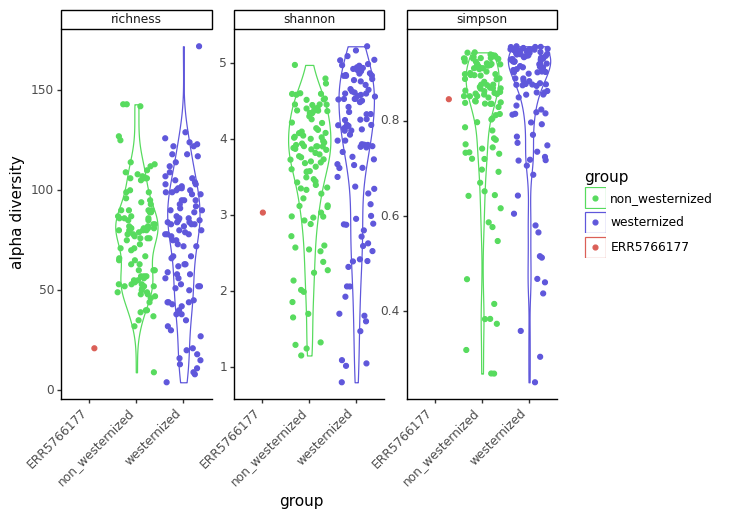
\includegraphics{assets/images/chapters/taxonomic-profiling/analysis_91_1.png}

}

\caption{png}

\end{figure}

\begin{verbatim}
<ggplot: (407407577)>
\end{verbatim}

\textbf{Pause and think: Why do we observe a smaller species richness
and diversity in our sample ?}

\hypertarget{beta-diversity}{%
\subsubsection{7.2.2 Beta diversity}\label{beta-diversity}}

The Beta diversity is the measure of diversity between a pair of
samples. It is used to compare the diversity between samples and see how
they relate.

We will compute the beta diversity using the
\href{https://en.wikipedia.org/wiki/Bray\%E2\%80\%93Curtis_dissimilarity}{bray-curtis}
dissimilarity

\begin{Shaded}
\begin{Highlighting}[]
\NormalTok{beta\_diversity }\OperatorTok{=}\NormalTok{ skbio.diversity.beta\_diversity(metric}\OperatorTok{=}\StringTok{\textquotesingle{}braycurtis\textquotesingle{}}\NormalTok{, counts}\OperatorTok{=}\NormalTok{all\_species.transpose(), ids}\OperatorTok{=}\NormalTok{all\_species.columns, validate}\OperatorTok{=}\VariableTok{True}\NormalTok{)}
\end{Highlighting}
\end{Shaded}

We get a distance matrix

\begin{Shaded}
\begin{Highlighting}[]
\BuiltInTok{print}\NormalTok{(beta\_diversity)}
\end{Highlighting}
\end{Shaded}

\begin{verbatim}
201x201 distance matrix
IDs:
'ERR5766177', 'de028ad4-7ae6-11e9-a106-68b59976a384', 'PNP_Main_283', ...
Data:
[[0.         1.         0.81508134 ... 0.85716612 0.69790092 0.8303726 ]
 [1.         0.         0.99988327 ... 0.99853413 0.994116   0.99877258]
 [0.81508134 0.99988327 0.         ... 0.82311942 0.87202543 0.91363156]
 ...
 [0.85716612 0.99853413 0.82311942 ... 0.         0.84253376 0.76616679]
 [0.69790092 0.994116   0.87202543 ... 0.84253376 0.         0.82409272]
 [0.8303726  0.99877258 0.91363156 ... 0.76616679 0.82409272 0.        ]]
\end{verbatim}

To visualize this distance matrix in a lower dimensional space, we'll
use a
\href{https://en.wikipedia.org/wiki/Multidimensional_scaling\#Types}{PCoA},
which is is a method very similar to a PCA, but taking a distance matrix
as input.

\begin{Shaded}
\begin{Highlighting}[]
\NormalTok{pcoa }\OperatorTok{=}\NormalTok{ skbio.stats.ordination.pcoa(beta\_diversity)}
\end{Highlighting}
\end{Shaded}

\begin{verbatim}
/Users/maxime/mambaforge/envs/summer_school_microbiome/lib/python3.9/site-packages/skbio/stats/ordination/_principal_coordinate_analysis.py:143: RuntimeWarning:
The result contains negative eigenvalues. Please compare their magnitude with the magnitude of some of the largest positive eigenvalues.
If the negative ones are smaller, it's probably safe to ignore them, but if they are large in magnitude, the results won't be useful.
See the Notes section for more details. The smallest eigenvalue is -0.25334842745723996 and the largest is 10.204440747987945.
\end{verbatim}

\begin{Shaded}
\begin{Highlighting}[]
\NormalTok{pcoa.samples}
\end{Highlighting}
\end{Shaded}

PC1

PC2

PC3

PC4

PC5

PC6

PC7

PC8

PC9

PC10

\ldots{}

PC192

PC193

PC194

PC195

PC196

PC197

PC198

PC199

PC200

PC201

ERR5766177

0.216901

-0.039778

0.107412

0.273272

0.020540

0.114876

-0.256332

-0.151069

0.097451

0.060211

\ldots{}

0.0

0.0

0.0

0.0

0.0

0.0

0.0

0.0

0.0

0.0

de028ad4-7ae6-11e9-a106-68b59976a384

-0.099355

0.145224

-0.191676

0.127626

0.119754

-0.132209

-0.097382

0.036728

0.081294

-0.056686

\ldots{}

0.0

0.0

0.0

0.0

0.0

0.0

0.0

0.0

0.0

0.0

PNP\_Main\_283

-0.214108

-0.147466

0.116027

0.090059

0.076644

0.111536

0.092115

0.026477

-0.006460

-0.018592

\ldots{}

0.0

0.0

0.0

0.0

0.0

0.0

0.0

0.0

0.0

0.0

PNP\_Validation\_55

0.244827

-0.173996

-0.311197

-0.012836

0.031759

0.117548

0.148715

-0.135641

0.034730

-0.009395

\ldots{}

0.0

0.0

0.0

0.0

0.0

0.0

0.0

0.0

0.0

0.0

G80275

-0.261358

-0.077147

-0.254374

-0.065932

0.088538

0.165970

-0.005260

-0.028739

-0.002016

0.015719

\ldots{}

0.0

0.0

0.0

0.0

0.0

0.0

0.0

0.0

0.0

0.0

\ldots{}

\ldots{}

\ldots{}

\ldots{}

\ldots{}

\ldots{}

\ldots{}

\ldots{}

\ldots{}

\ldots{}

\ldots{}

\ldots{}

\ldots{}

\ldots{}

\ldots{}

\ldots{}

\ldots{}

\ldots{}

\ldots{}

\ldots{}

\ldots{}

\ldots{}

KHG\_9

0.296057

-0.150300

0.013941

0.032649

-0.147692

0.019663

-0.063120

-0.034453

-0.073514

0.070085

\ldots{}

0.0

0.0

0.0

0.0

0.0

0.0

0.0

0.0

0.0

0.0

A48\_01\_1FE

0.110621

0.030971

0.154231

-0.185961

-0.008512

-0.103420

0.028169

-0.044530

0.041902

0.068597

\ldots{}

0.0

0.0

0.0

0.0

0.0

0.0

0.0

0.0

0.0

0.0

KHG\_1

-0.100009

0.167885

0.009915

0.076842

-0.405582

-0.039111

-0.006421

-0.009774

-0.072252

0.150000

\ldots{}

0.0

0.0

0.0

0.0

0.0

0.0

0.0

0.0

0.0

0.0

TZ\_81781

0.405716

-0.139297

-0.075026

-0.079716

-0.053264

-0.119271

0.068261

-0.018821

0.198152

-0.012792

\ldots{}

0.0

0.0

0.0

0.0

0.0

0.0

0.0

0.0

0.0

0.0

A09\_01\_1FE

0.089101

0.471135

0.069629

-0.125644

-0.036793

0.115151

0.060507

-0.000912

-0.027239

-0.138436

\ldots{}

0.0

0.0

0.0

0.0

0.0

0.0

0.0

0.0

0.0

0.0

201 rows × 201 columns

Let's look at the variance explained by the first axes by using a scree
plot

\begin{Shaded}
\begin{Highlighting}[]
\NormalTok{var\_explained }\OperatorTok{=}\NormalTok{ pcoa.proportion\_explained[:}\DecValTok{9}\NormalTok{].to\_frame(name}\OperatorTok{=}\StringTok{\textquotesingle{}variance explained\textquotesingle{}}\NormalTok{).reset\_index().rename(columns}\OperatorTok{=}\NormalTok{\{}\StringTok{\textquotesingle{}index\textquotesingle{}}\NormalTok{:}\StringTok{\textquotesingle{}PC\textquotesingle{}}\NormalTok{\})}
\end{Highlighting}
\end{Shaded}

\begin{Shaded}
\begin{Highlighting}[]
\NormalTok{ggplot(var\_explained, aes(x}\OperatorTok{=}\StringTok{\textquotesingle{}PC\textquotesingle{}}\NormalTok{, y}\OperatorTok{=}\StringTok{\textquotesingle{}variance explained\textquotesingle{}}\NormalTok{, group}\OperatorTok{=}\DecValTok{1}\NormalTok{)) }\OperatorTok{\textbackslash{}}
\OperatorTok{+}\NormalTok{ geom\_point() }\OperatorTok{\textbackslash{}}
\OperatorTok{+}\NormalTok{ geom\_line() }\OperatorTok{\textbackslash{}}
\OperatorTok{+}\NormalTok{ theme\_classic()}
\end{Highlighting}
\end{Shaded}

\begin{figure}

{\centering 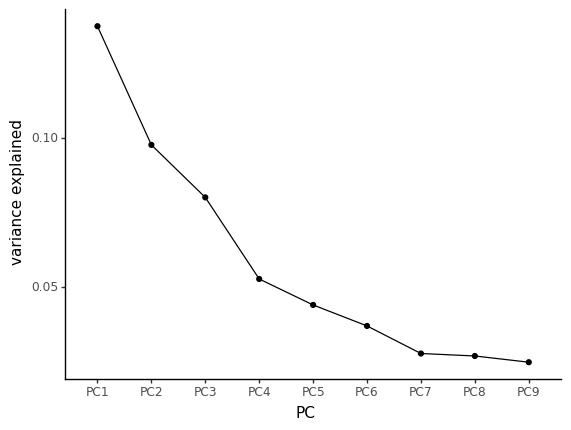
\includegraphics{assets/images/chapters/taxonomic-profiling/analysis_102_0.png}

}

\caption{png}

\end{figure}

\begin{verbatim}
<ggplot: (407531271)>
\end{verbatim}

In this scree plot, we're looking for the ``elbow'', where there is a
drop in the slope. Here, it seems that most of the variance is captures
by the 3 first principal components

\begin{Shaded}
\begin{Highlighting}[]
\NormalTok{pcoa\_embed }\OperatorTok{=}\NormalTok{ pcoa.samples[[}\StringTok{\textquotesingle{}PC1\textquotesingle{}}\NormalTok{,}\StringTok{\textquotesingle{}PC2\textquotesingle{}}\NormalTok{,}\StringTok{\textquotesingle{}PC3\textquotesingle{}}\NormalTok{]].rename\_axis(}\StringTok{\textquotesingle{}sample\textquotesingle{}}\NormalTok{).reset\_index()}
\end{Highlighting}
\end{Shaded}

\begin{Shaded}
\begin{Highlighting}[]
\NormalTok{pcoa\_embed }\OperatorTok{=}\NormalTok{ (}
\NormalTok{    pcoa\_embed}
\NormalTok{    .merge(metadata[[}\StringTok{\textquotesingle{}sample\_id\textquotesingle{}}\NormalTok{, }\StringTok{\textquotesingle{}non\_westernized\textquotesingle{}}\NormalTok{]], left\_on}\OperatorTok{=}\StringTok{\textquotesingle{}sample\textquotesingle{}}\NormalTok{, right\_on}\OperatorTok{=}\StringTok{\textquotesingle{}sample\_id\textquotesingle{}}\NormalTok{, how}\OperatorTok{=}\StringTok{\textquotesingle{}outer\textquotesingle{}}\NormalTok{)}
\NormalTok{    .drop(}\StringTok{\textquotesingle{}sample\_id\textquotesingle{}}\NormalTok{, axis}\OperatorTok{=}\DecValTok{1}\NormalTok{)}
\NormalTok{    .rename(columns}\OperatorTok{=}\NormalTok{\{}\StringTok{\textquotesingle{}non\_westernized\textquotesingle{}}\NormalTok{:}\StringTok{\textquotesingle{}group\textquotesingle{}}\NormalTok{\})}
\NormalTok{)}
\NormalTok{pcoa\_embed[}\StringTok{\textquotesingle{}group\textquotesingle{}}\NormalTok{] }\OperatorTok{=}\NormalTok{ pcoa\_embed[}\StringTok{\textquotesingle{}group\textquotesingle{}}\NormalTok{].replace(\{}\StringTok{\textquotesingle{}yes\textquotesingle{}}\NormalTok{:}\StringTok{\textquotesingle{}non\_westernized\textquotesingle{}}\NormalTok{,}\StringTok{\textquotesingle{}no\textquotesingle{}}\NormalTok{:}\StringTok{\textquotesingle{}westernized\textquotesingle{}}\NormalTok{, pd.NA:}\StringTok{\textquotesingle{}ERR5766177\textquotesingle{}}\NormalTok{\})}
\end{Highlighting}
\end{Shaded}

Let's first look at these components with 2D plots

\begin{Shaded}
\begin{Highlighting}[]
\NormalTok{ggplot(pcoa\_embed, aes(x}\OperatorTok{=}\StringTok{\textquotesingle{}PC1\textquotesingle{}}\NormalTok{, y}\OperatorTok{=}\StringTok{\textquotesingle{}PC2\textquotesingle{}}\NormalTok{, color}\OperatorTok{=}\StringTok{\textquotesingle{}group\textquotesingle{}}\NormalTok{)) }\OperatorTok{\textbackslash{}}
\OperatorTok{+}\NormalTok{ geom\_point() }\OperatorTok{\textbackslash{}}
\OperatorTok{+}\NormalTok{ theme\_classic() }\OperatorTok{\textbackslash{}}
\OperatorTok{+}\NormalTok{ scale\_color\_manual(\{}\StringTok{\textquotesingle{}ERR5766177\textquotesingle{}}\NormalTok{:}\StringTok{\textquotesingle{}\#DB5F57\textquotesingle{}}\NormalTok{,}\StringTok{\textquotesingle{}westernized\textquotesingle{}}\NormalTok{:}\StringTok{\textquotesingle{}\#5F57DB\textquotesingle{}}\NormalTok{,}\StringTok{\textquotesingle{}non\_westernized\textquotesingle{}}\NormalTok{:}\StringTok{\textquotesingle{}\#57DB5E\textquotesingle{}}\NormalTok{\})}
\end{Highlighting}
\end{Shaded}

\begin{figure}

{\centering 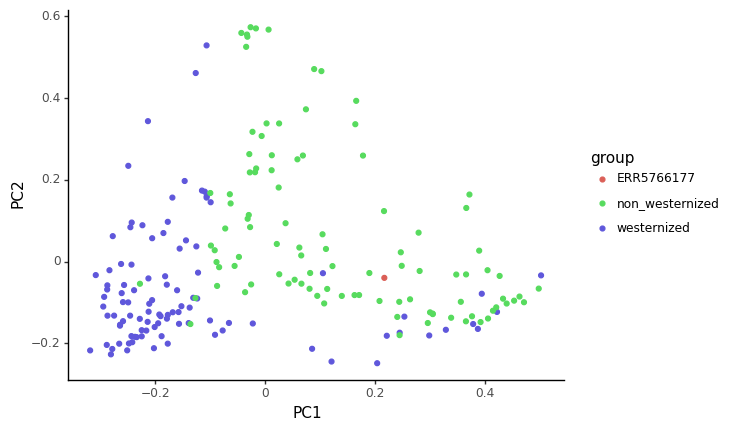
\includegraphics{assets/images/chapters/taxonomic-profiling/analysis_107_0.png}

}

\caption{png}

\end{figure}

\begin{verbatim}
<ggplot: (407572134)>
\end{verbatim}

\begin{Shaded}
\begin{Highlighting}[]
\NormalTok{ggplot(pcoa\_embed, aes(x}\OperatorTok{=}\StringTok{\textquotesingle{}PC1\textquotesingle{}}\NormalTok{, y}\OperatorTok{=}\StringTok{\textquotesingle{}PC3\textquotesingle{}}\NormalTok{, color}\OperatorTok{=}\StringTok{\textquotesingle{}group\textquotesingle{}}\NormalTok{)) }\OperatorTok{+}
\NormalTok{geom\_point() }\OperatorTok{+}
\NormalTok{theme\_classic() }\OperatorTok{+}
\NormalTok{scale\_color\_manual(\{}\StringTok{\textquotesingle{}ERR5766177\textquotesingle{}}\NormalTok{:}\StringTok{\textquotesingle{}\#DB5F57\textquotesingle{}}\NormalTok{,}\StringTok{\textquotesingle{}westernized\textquotesingle{}}\NormalTok{:}\StringTok{\textquotesingle{}\#5F57DB\textquotesingle{}}\NormalTok{,}\StringTok{\textquotesingle{}non\_westernized\textquotesingle{}}\NormalTok{:}\StringTok{\textquotesingle{}\#57DB5E\textquotesingle{}}\NormalTok{\})}
\end{Highlighting}
\end{Shaded}

\begin{figure}

{\centering 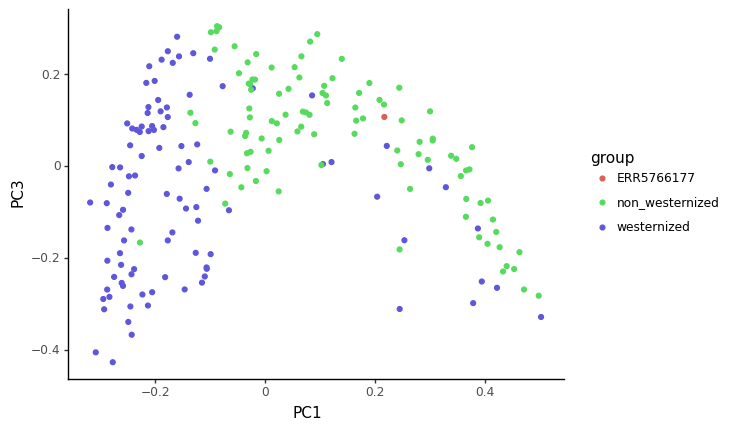
\includegraphics{assets/images/chapters/taxonomic-profiling/analysis_108_0.png}

}

\caption{png}

\end{figure}

\begin{verbatim}
<ggplot: (407612651)>
\end{verbatim}

Then with a 3d plot

\begin{Shaded}
\begin{Highlighting}[]
\ImportTok{import}\NormalTok{ plotly.express }\ImportTok{as}\NormalTok{ px}

\NormalTok{fig }\OperatorTok{=}\NormalTok{ px.scatter\_3d(pcoa\_embed, x}\OperatorTok{=}\StringTok{"PC1"}\NormalTok{, y}\OperatorTok{=}\StringTok{"PC2"}\NormalTok{, z}\OperatorTok{=}\StringTok{"PC3"}\NormalTok{,}
\NormalTok{                  color }\OperatorTok{=} \StringTok{"group"}\NormalTok{,}
\NormalTok{                  color\_discrete\_map}\OperatorTok{=}\NormalTok{\{}\StringTok{\textquotesingle{}ERR5766177\textquotesingle{}}\NormalTok{:}\StringTok{\textquotesingle{}\#DB5F57\textquotesingle{}}\NormalTok{,}\StringTok{\textquotesingle{}westernized\textquotesingle{}}\NormalTok{:}\StringTok{\textquotesingle{}\#5F57DB\textquotesingle{}}\NormalTok{,}\StringTok{\textquotesingle{}non\_westernized\textquotesingle{}}\NormalTok{:}\StringTok{\textquotesingle{}\#57DB5E\textquotesingle{}}\NormalTok{\},}
\NormalTok{                  hover\_name}\OperatorTok{=}\StringTok{"sample"}\NormalTok{)}
\NormalTok{fig.show()}
\end{Highlighting}
\end{Shaded}

\begin{tcolorbox}[enhanced jigsaw, opacitybacktitle=0.6, bottomtitle=1mm, opacityback=0, colback=white, coltitle=black, leftrule=.75mm, toprule=.15mm, title=\textcolor{quarto-callout-important-color}{\faExclamation}\hspace{0.5em}{Important}, colframe=quarto-callout-important-color-frame, toptitle=1mm, arc=.35mm, left=2mm, titlerule=0mm, breakable, rightrule=.15mm, bottomrule=.15mm, colbacktitle=quarto-callout-important-color!10!white]

3D PLOT HERE NOT DISPLAYED DUE TO RENDERING LIMITATIONS - PLEASE SEE
JUPYTER NOTEBOOK

\end{tcolorbox}

\textbf{Pause and think: How do you think this embedding represents how
our sample relates to modern reference samples ?}

We can also visualize this distance matrix using a clustered heatmap,
where pairs of sample with a small beta diversity are clustered together

\begin{Shaded}
\begin{Highlighting}[]
\ImportTok{import}\NormalTok{ seaborn }\ImportTok{as}\NormalTok{ sns}
\ImportTok{import}\NormalTok{ scipy.spatial }\ImportTok{as}\NormalTok{ sp, scipy.cluster.hierarchy }\ImportTok{as}\NormalTok{ hc}
\end{Highlighting}
\end{Shaded}

\begin{Shaded}
\begin{Highlighting}[]
\NormalTok{pcoa\_embed[}\StringTok{\textquotesingle{}colour\textquotesingle{}}\NormalTok{] }\OperatorTok{=}\NormalTok{ pcoa\_embed[}\StringTok{\textquotesingle{}group\textquotesingle{}}\NormalTok{].}\BuiltInTok{map}\NormalTok{(\{}\StringTok{\textquotesingle{}ERR5766177\textquotesingle{}}\NormalTok{:}\StringTok{\textquotesingle{}\#DB5F57\textquotesingle{}}\NormalTok{,}\StringTok{\textquotesingle{}westernized\textquotesingle{}}\NormalTok{:}\StringTok{\textquotesingle{}\#5F57DB\textquotesingle{}}\NormalTok{,}\StringTok{\textquotesingle{}non\_westernized\textquotesingle{}}\NormalTok{:}\StringTok{\textquotesingle{}\#57DB5E\textquotesingle{}}\NormalTok{\})}
\end{Highlighting}
\end{Shaded}

\begin{Shaded}
\begin{Highlighting}[]
\NormalTok{linkage }\OperatorTok{=}\NormalTok{ hc.linkage(sp.distance.squareform(beta\_diversity.to\_data\_frame()), method}\OperatorTok{=}\StringTok{\textquotesingle{}average\textquotesingle{}}\NormalTok{)}

\NormalTok{sns.clustermap(}
\NormalTok{    beta\_diversity.to\_data\_frame(),}
\NormalTok{    row\_linkage}\OperatorTok{=}\NormalTok{linkage,}
\NormalTok{    col\_linkage}\OperatorTok{=}\NormalTok{linkage,}
\NormalTok{    row\_colors }\OperatorTok{=}\NormalTok{ pcoa\_embed[}\StringTok{\textquotesingle{}colour\textquotesingle{}}\NormalTok{].to\_list()}
\NormalTok{)}
\end{Highlighting}
\end{Shaded}

\begin{verbatim}
<seaborn.matrix.ClusterGrid at 0x185b56100>
\end{verbatim}

\begin{figure}

{\centering \includegraphics{assets/images/chapters/taxonomic-profiling/analysis_115_1.png}

}

\caption{png}

\end{figure}

\hypertarget{additional-steps}{%
\subsection{8. Additional steps}\label{additional-steps}}

\hypertarget{source-tracking}{%
\subsubsection{8.1 Source tracking}\label{source-tracking}}

Sourcetracker is a program that can estimate the proportion of different
sources (reference biomes) contained in a sample (a sink). However,
because of the statistical framework that it uses (MCMC with
\href{https://en.wikipedia.org/wiki/Gibbs_sampling\#:~:text=In\%20statistics\%2C\%20Gibbs\%20sampling\%20or,when\%20direct\%20sampling\%20is\%20difficult.}{Gibbs
sampling}), we recommend to limit the number of source samples to
greatly reduce runtime

First, you will need to transform our relative abundance table to counts
for SourceTracker

\begin{Shaded}
\begin{Highlighting}[]
\NormalTok{all\_species\_counts }\OperatorTok{=}\NormalTok{ all\_species.multiply(}\DecValTok{1000000}\NormalTok{).astype(}\BuiltInTok{int}\NormalTok{)}
\end{Highlighting}
\end{Shaded}

\begin{Shaded}
\begin{Highlighting}[]
\NormalTok{min\_count }\OperatorTok{=}\NormalTok{ all\_species\_counts.}\BuiltInTok{sum}\NormalTok{(axis}\OperatorTok{=}\DecValTok{0}\NormalTok{).}\BuiltInTok{min}\NormalTok{()}
\NormalTok{min\_count}
\end{Highlighting}
\end{Shaded}

\begin{verbatim}
95327810
\end{verbatim}

Exporting the count table to \texttt{tsv}

\begin{Shaded}
\begin{Highlighting}[]
\NormalTok{all\_species\_counts.to\_csv(}\StringTok{"../results/sourcetracker2/all\_species\_counts.tsv"}\NormalTok{, sep}\OperatorTok{=}\StringTok{"}\CharTok{\textbackslash{}t}\StringTok{"}\NormalTok{, index\_label}\OperatorTok{=}\StringTok{\textquotesingle{}Taxon\textquotesingle{}}\NormalTok{)}
\end{Highlighting}
\end{Shaded}

Converting to \href{https://biom-format.org/}{\texttt{biom} format}

\begin{Shaded}
\begin{Highlighting}[]
\OperatorTok{!}\NormalTok{biom convert }\OperatorTok{{-}}\NormalTok{i ..}\OperatorTok{/}\NormalTok{results}\OperatorTok{/}\NormalTok{sourcetracker2}\OperatorTok{/}\NormalTok{all\_species\_counts.tsv }\OperatorTok{\textbackslash{}}
\OperatorTok{{-}}\NormalTok{o ..}\OperatorTok{/}\NormalTok{results}\OperatorTok{/}\NormalTok{sourcetracker2}\OperatorTok{/}\NormalTok{all\_species\_counts.biom }\OperatorTok{\textbackslash{}}
\OperatorTok{{-}{-}}\NormalTok{table}\OperatorTok{{-}}\BuiltInTok{type}\OperatorTok{=}\StringTok{"Taxon table"} \OperatorTok{{-}{-}}\NormalTok{to}\OperatorTok{{-}}\NormalTok{hdf5}
\end{Highlighting}
\end{Shaded}

Converting the metadata to Sourtracker format

\begin{Shaded}
\begin{Highlighting}[]
\NormalTok{st2\_metadata }\OperatorTok{=}\NormalTok{ metadata[[}\StringTok{\textquotesingle{}sample\_id\textquotesingle{}}\NormalTok{, }\StringTok{\textquotesingle{}non\_westernized\textquotesingle{}}\NormalTok{]].rename(columns}\OperatorTok{=}\NormalTok{\{}\StringTok{\textquotesingle{}non\_westernized\textquotesingle{}}\NormalTok{:}\StringTok{\textquotesingle{}Env\textquotesingle{}}\NormalTok{, }\StringTok{\textquotesingle{}sample\_id\textquotesingle{}}\NormalTok{:}\StringTok{\textquotesingle{}\#SampleID\textquotesingle{}}\NormalTok{\})}
\NormalTok{st2\_metadata[}\StringTok{\textquotesingle{}Env\textquotesingle{}}\NormalTok{] }\OperatorTok{=}\NormalTok{ st2\_metadata[}\StringTok{\textquotesingle{}Env\textquotesingle{}}\NormalTok{].replace(\{}\StringTok{\textquotesingle{}yes\textquotesingle{}}\NormalTok{:}\StringTok{\textquotesingle{}non\_westernized\textquotesingle{}}\NormalTok{,}\StringTok{\textquotesingle{}no\textquotesingle{}}\NormalTok{:}\StringTok{\textquotesingle{}westernized\textquotesingle{}}\NormalTok{\})}
\NormalTok{st2\_metadata[}\StringTok{\textquotesingle{}SourceSink\textquotesingle{}}\NormalTok{] }\OperatorTok{=}\NormalTok{ [}\StringTok{\textquotesingle{}source\textquotesingle{}}\NormalTok{] }\OperatorTok{*}\NormalTok{ st2\_metadata.shape[}\DecValTok{0}\NormalTok{]}
\end{Highlighting}
\end{Shaded}

We subset it to select only 10 samples from each source

\begin{Shaded}
\begin{Highlighting}[]
\NormalTok{st2\_metadata }\OperatorTok{=}\NormalTok{ st2\_metadata.groupby(}\StringTok{\textquotesingle{}Env\textquotesingle{}}\NormalTok{).sample(}\DecValTok{10}\NormalTok{).reset\_index()}
\end{Highlighting}
\end{Shaded}

\begin{Shaded}
\begin{Highlighting}[]
\NormalTok{st2\_metadata }\OperatorTok{=}\NormalTok{ st2\_metadata.append(\{}\StringTok{\textquotesingle{}\#SampleID\textquotesingle{}}\NormalTok{:}\StringTok{\textquotesingle{}ERR5766177\textquotesingle{}}\NormalTok{, }\StringTok{\textquotesingle{}Env\textquotesingle{}}\NormalTok{:}\StringTok{\textquotesingle{}{-}\textquotesingle{}}\NormalTok{,}\StringTok{\textquotesingle{}SourceSink\textquotesingle{}}\NormalTok{:}\StringTok{\textquotesingle{}sink\textquotesingle{}}\NormalTok{\},}
\NormalTok{                                   ignore\_index}\OperatorTok{=}\VariableTok{True}\NormalTok{)[[}\StringTok{\textquotesingle{}\#SampleID\textquotesingle{}}\NormalTok{,}\StringTok{\textquotesingle{}SourceSink\textquotesingle{}}\NormalTok{,}\StringTok{\textquotesingle{}Env\textquotesingle{}}\NormalTok{]].set\_index(}\StringTok{\textquotesingle{}\#SampleID\textquotesingle{}}\NormalTok{)}
\end{Highlighting}
\end{Shaded}

\begin{verbatim}
/var/folders/1c/l1qb09f15jddsh65f6xv1n_r0000gp/T/ipykernel_40830/2882312005.py:1: FutureWarning:

The frame.append method is deprecated and will be removed from pandas in a future version. Use pandas.concat instead.
\end{verbatim}

\begin{Shaded}
\begin{Highlighting}[]
\NormalTok{st2\_metadata.to\_csv(}\StringTok{"../results/sourcetracker2/labels\_st2.tsv"}\NormalTok{, sep}\OperatorTok{=}\StringTok{"}\CharTok{\textbackslash{}t}\StringTok{"}\NormalTok{, index\_label}\OperatorTok{=}\StringTok{\textquotesingle{}\#SampleID\textquotesingle{}}\NormalTok{)}
\end{Highlighting}
\end{Shaded}

\begin{Shaded}
\begin{Highlighting}[]
\ExtensionTok{sourcetracker2}\NormalTok{ gibbs }\DataTypeTok{\textbackslash{}}
    \AttributeTok{{-}i}\NormalTok{ ../results/sourcetracker2/all\_species\_counts.biom }\DataTypeTok{\textbackslash{}}
    \AttributeTok{{-}m}\NormalTok{ ../results/sourcetracker2/labels\_st2.tsv }\DataTypeTok{\textbackslash{}}
    \AttributeTok{{-}o}\NormalTok{ ../results/sourcetracker2/st2 }\DataTypeTok{\textbackslash{}}
    \AttributeTok{{-}{-}source\_rarefaction\_depth}\NormalTok{ 95327810 }\DataTypeTok{\textbackslash{}}
    \AttributeTok{{-}{-}sink\_rarefaction\_depth}\NormalTok{ 95327810 }\DataTypeTok{\textbackslash{}}
    \AttributeTok{{-}{-}jobs}\NormalTok{ 10}
\end{Highlighting}
\end{Shaded}

\textbf{Because SourceTracker is relying on MCMC sampling, it can very
slow to run (which is why we won't run it here)}

Among alternative faster solutions for source tracking are (among
others):

\begin{itemize}
\tightlist
\item
  FEAST (\href{https://doi.org/10.1038/s41592-019-0431-x}{article},
  \href{https://github.com/cozygene/FEAST}{code}),
\item
  Sourcepredict (\href{https://doi.org/10.21105/joss.01540}{article},
  \href{https://github.com/maxibor/sourcepredict}{code})
\end{itemize}

\hypertarget{the-next-steps}{%
\subsubsection{8.2 The next steps:}\label{the-next-steps}}

\begin{itemize}
\tightlist
\item
  Damage Analysis
  (\href{https://ginolhac.github.io/mapDamage/}{mapDamage},
  \href{https://github.com/Integrative-Transcriptomics/DamageProfiler}{DamageProfiler},
  \href{https://github.com/maxibor/pydamage}{PyDamage})
\item
  Assembly (\href{https://github.com/voutcn/megahit}{megahit},
  \href{https://github.com/ablab/spades}{metaSPAdes}), binning
  (\href{https://bitbucket.org/berkeleylab/metabat/src/master/}{metabat2},
  \href{https://sourceforge.net/projects/maxbin2/}{maxbin2},
  \href{https://github.com/cmks/DAS_Tool}{dastool}), and bin validation
  (\href{https://github.com/Ecogenomics/CheckM}{checkm},
  \href{https://github.com/grp-bork/gunc}{gunc})
\item
  Functional analysis
  (\href{https://github.com/tseemann/prokka}{Prokka},
  \href{https://github.com/biobakery/humann}{Humann})
\item
  Differential abundance
  (\href{https://github.com/biobakery/Maaslin2}{Maaslin2},
  \href{https://github.com/biobakery/lefse}{Lefse},
  \href{https://github.com/biocore/songbird}{Songbird}, GLM, Mixed
  effect models). Nice review by
  \href{https://doi.org/10.1186/s12859-021-04193-6}{Wallen 2021}
\item
  genotyping
\item
  Phylogenies
\item
  \ldots{}
\end{itemize}

\hypertarget{functional-profiling-1}{%
\chapter{Functional Profiling}\label{functional-profiling-1}}

\begin{tcolorbox}[enhanced jigsaw, opacitybacktitle=0.6, bottomtitle=1mm, opacityback=0, colback=white, coltitle=black, leftrule=.75mm, toprule=.15mm, title=\textcolor{quarto-callout-tip-color}{\faLightbulb}\hspace{0.5em}{Tip}, colframe=quarto-callout-tip-color-frame, toptitle=1mm, arc=.35mm, left=2mm, titlerule=0mm, breakable, rightrule=.15mm, bottomrule=.15mm, colbacktitle=quarto-callout-tip-color!10!white]

For this chapter's exercises, if not already performed, you will need to
create the \protect\hyperlink{creating-a-conda-environment}{conda
environment} from the \texttt{yml} file in the following
\href{https://doi.org/10.5281/zenodo.6983188}{archive}, and activate the
environment:

\begin{Shaded}
\begin{Highlighting}[]
\ExtensionTok{conda}\NormalTok{ activate phylogenomics{-}functional}
\end{Highlighting}
\end{Shaded}

\end{tcolorbox}

\hypertarget{lecture-10}{%
\section{Lecture}\label{lecture-10}}

PDF version of these slides can be downloaded from
\href{https://github.com/SPAAM-community/wss-summer-school/raw/main/docs/assets/slides/2022/5c-intro-to-functional-analysis/SPAAM\%20Summer\%20School\%202022\%20-\%205C\%20-\%20Function\%20Analysis.pdf}{here}.

\hypertarget{preparation}{%
\section{Preparation}\label{preparation}}

The data and conda environment \texttt{.yaml} file for this practical
session can be downloaded from here:
\url{https://doi.org/10.5281/zenodo.6983188}. See instructions on page.

Change into the session directory

\begin{Shaded}
\begin{Highlighting}[]
\BuiltInTok{cd}\NormalTok{ /}\OperatorTok{\textless{}}\NormalTok{path}\OperatorTok{\textgreater{}}\NormalTok{/}\OperatorTok{\textless{}}\NormalTok{to}\OperatorTok{\textgreater{}}\NormalTok{/5c{-}functional{-}genomics/}
\end{Highlighting}
\end{Shaded}

Load the conda environment.

\begin{Shaded}
\begin{Highlighting}[]
\ExtensionTok{conda}\NormalTok{ activate phylogenomics{-}functional}
\end{Highlighting}
\end{Shaded}

Open R Studio from within the conda environment, and we can load the
required libraries for this walkthrough.

\begin{Shaded}
\begin{Highlighting}[]
\FunctionTok{library}\NormalTok{(mixOmics) }\DocumentationTok{\#\# For PCA generation}

\DocumentationTok{\#\# Utility packages (pretty stuff)}
\FunctionTok{library}\NormalTok{(knitr)}
\FunctionTok{library}\NormalTok{(data.table)}
\FunctionTok{library}\NormalTok{(tidyverse)}
\FunctionTok{library}\NormalTok{(gplots)}
\FunctionTok{library}\NormalTok{(ggrepel)}
\FunctionTok{library}\NormalTok{(viridis)}
\FunctionTok{library}\NormalTok{(patchwork)}
\end{Highlighting}
\end{Shaded}

\hypertarget{humann3-pathways}{%
\section{HUMAnN3 Pathways}\label{humann3-pathways}}

First, we need to run HUMMAn3 to align reads against gene databases and
convert to gene family names counts.

\begin{tcolorbox}[enhanced jigsaw, opacitybacktitle=0.6, bottomtitle=1mm, opacityback=0, colback=white, coltitle=black, leftrule=.75mm, toprule=.15mm, title=\textcolor{quarto-callout-warning-color}{\faExclamationTriangle}\hspace{0.5em}{Warning}, colframe=quarto-callout-warning-color-frame, toptitle=1mm, arc=.35mm, left=2mm, titlerule=0mm, breakable, rightrule=.15mm, bottomrule=.15mm, colbacktitle=quarto-callout-warning-color!10!white]

We will not run HUMANn3 here as it requires very large databases and
takes a long time to run, so we will give you the commands you normally
would run but we provide with you pre-made results files before you (see
below).

\begin{Shaded}
\begin{Highlighting}[]
\CommentTok{\#\# DO NOT RUN!}

\CommentTok{\# run humann3}
\ExtensionTok{humann3} \AttributeTok{{-}{-}input}\NormalTok{ file.fastq }\AttributeTok{{-}{-}output}\NormalTok{ output }\AttributeTok{{-}{-}threads} \OperatorTok{\textless{}}\NormalTok{threads}\OperatorTok{\textgreater{}}

\CommentTok{\# join all output tables (can do for both gene and pathways)}
\ExtensionTok{humann\_join\_tables} \AttributeTok{{-}i}\NormalTok{ output/ }\AttributeTok{{-}o}\NormalTok{ genefamilies\_joined.tsv }\AttributeTok{{-}{-}file\_name}\NormalTok{ unmapped\_genefamilies}

\CommentTok{\# normalize the output (here by tss {-} total sum scaling, can do for both gene and pathways)}
\ExtensionTok{humann\_renorm\_table} \AttributeTok{{-}{-}input}\NormalTok{ genefamilies\_joined.tsv }\AttributeTok{{-}{-}output}\NormalTok{ genefamilies\_joined\_cpm.tsv }\AttributeTok{{-}{-}units}\NormalTok{ tss}

\CommentTok{\# regroup the table to combine gene families (standardise gene family IDs across taxa)}
\ExtensionTok{humann\_regroup\_table} \AttributeTok{{-}{-}input}\NormalTok{ genefamilies\_joined\_cpm.tsv }\AttributeTok{{-}{-}output}\NormalTok{ genefamilies\_joined\_cpm\_ur90rxn.tsv }\AttributeTok{{-}{-}groups}\NormalTok{ uniref90\_rxn}

\CommentTok{\# give the gene families names}
\ExtensionTok{humann\_rename\_table} \AttributeTok{{-}{-}input}\NormalTok{ genefamilies\_joined\_cpm\_ur90rxn.tsv }\AttributeTok{{-}{-}output}\NormalTok{ genefamilies\_joined\_cpm\_ur90rxn\_names.tsv }\AttributeTok{{-}n}\NormalTok{ metacyc{-}rxn}
\end{Highlighting}
\end{Shaded}

\end{tcolorbox}

\hypertarget{humann3-tables}{%
\section{humann3 tables}\label{humann3-tables}}

First lets load a pre-made pathway abundance file

\begin{Shaded}
\begin{Highlighting}[]
\DocumentationTok{\#\# load the species and genus tables generated with humann3}
\NormalTok{humann3\_path\_full }\OtherTok{\textless{}{-}} \FunctionTok{fread}\NormalTok{(}\StringTok{"./pathabundance\_joined\_cpm.tsv"}\NormalTok{)}
\NormalTok{humann3\_path\_full }\OtherTok{\textless{}{-}} \FunctionTok{as\_tibble}\NormalTok{(humann3\_path\_full)}

\CommentTok{\# clean the file names}
\NormalTok{humann3\_path\_full }\OtherTok{\textless{}{-}} \FunctionTok{rename}\NormalTok{(humann3\_path\_full, }\AttributeTok{Pathway =} \StringTok{\textasciigrave{}}\AttributeTok{\# Pathway}\StringTok{\textasciigrave{}}\NormalTok{)}
\FunctionTok{colnames}\NormalTok{(humann3\_path\_full) }\OtherTok{\textless{}{-}} \FunctionTok{gsub}\NormalTok{(}\StringTok{".unmapped\_Abundance"}\NormalTok{,}\StringTok{""}\NormalTok{, }\FunctionTok{colnames}\NormalTok{(humann3\_path\_full))}
\FunctionTok{colnames}\NormalTok{(humann3\_path\_full) }\OtherTok{\textless{}{-}} \FunctionTok{gsub}\NormalTok{(}\StringTok{".SG1"}\NormalTok{,}\StringTok{""}\NormalTok{, }\FunctionTok{colnames}\NormalTok{(humann3\_path\_full))}

\CommentTok{\# remove unmapped and ungrouped reads}
\NormalTok{humann3\_path }\OtherTok{\textless{}{-}}\NormalTok{ humann3\_path\_full }\SpecialCharTok{\%\textgreater{}\%} \FunctionTok{filter}\NormalTok{(}\SpecialCharTok{!}\FunctionTok{str\_detect}\NormalTok{(Pathway, }\StringTok{"UNMAPPED|UNINTEGRATED"}\NormalTok{))}
\end{Highlighting}
\end{Shaded}

Then lets load associated sample metadata to help make it easier for
comparative analysis and make actual informative inferences.

The data being used in this session, is from
\href{https://doi.org/10.1093/pnasnexus/pgac148}{Velsko et al.~2022
(PNAS Nexus)}, where we tried to find associations between dental
pathologies and taxonomic and genome content. We had a large skeletal
collection from a single site in the Netherlands, with a lot of
osteological metadata. The study aimed to see if there were any links
between the oral microbiome and groups of dental pathologies.

\begin{Shaded}
\begin{Highlighting}[]
\CommentTok{\# load the metadata file}
\NormalTok{full\_metadata }\OtherTok{\textless{}{-}} \FunctionTok{fread}\NormalTok{(}\StringTok{"full\_combined\_metadata.tsv"}\NormalTok{)}


\DocumentationTok{\#\# Example of metadata}
\FunctionTok{tibble}\NormalTok{(full\_metadata }\SpecialCharTok{\%\textgreater{}\%}
    \FunctionTok{filter}\NormalTok{(Site\_code }\SpecialCharTok{==} \StringTok{"MID"}\NormalTok{) }\SpecialCharTok{\%\textgreater{}\%}
    \FunctionTok{select}\NormalTok{(Site, Time\_period, Library\_ID, Sequencing\_instrument, Pipenotch, Max\_Perio\_Score, }\StringTok{\textasciigrave{}}\AttributeTok{\%teeth\_with\_caries}\StringTok{\textasciigrave{}}\NormalTok{))}
\end{Highlighting}
\end{Shaded}

First step: we can pre-define various functions for generate PCAs we
will use downstream - you don't have to worry about these too much they
are just custom functions to quickly plot PCAs from a \texttt{mixOmics}
PCA output object with ggplot, but we leave the code here for if you're
curious.

\begin{Shaded}
\begin{Highlighting}[]
\CommentTok{\# plot PCA with colored dots and the title including the \# of species or genera}
\NormalTok{plot\_pca }\OtherTok{\textless{}{-}} \ControlFlowTok{function}\NormalTok{(df, pc1, pc2, color\_group, shape\_group, ncomps) \{}
\NormalTok{    metadata\_group\_colors }\OtherTok{\textless{}{-}} \FunctionTok{get}\NormalTok{(}\FunctionTok{paste}\NormalTok{(color\_group, }\StringTok{"\_colors"}\NormalTok{, }\AttributeTok{sep =} \StringTok{""}\NormalTok{))}
\NormalTok{    metadata\_group\_shapes }\OtherTok{\textless{}{-}} \FunctionTok{get}\NormalTok{(}\FunctionTok{paste}\NormalTok{(shape\_group, }\StringTok{"\_shapes"}\NormalTok{, }\AttributeTok{sep =} \StringTok{""}\NormalTok{))}

\NormalTok{    pca.list }\OtherTok{\textless{}{-}}\NormalTok{ mixOmics}\SpecialCharTok{::}\FunctionTok{pca}\NormalTok{(df, }\AttributeTok{ncomp =}\NormalTok{ ncomps, }\AttributeTok{logratio =} \StringTok{\textquotesingle{}CLR\textquotesingle{}}\NormalTok{)}

    \DocumentationTok{\#\# Pull out loadings}
\NormalTok{    exp\_var }\OtherTok{\textless{}{-}} \FunctionTok{paste0}\NormalTok{(}\FunctionTok{round}\NormalTok{(pca.list}\SpecialCharTok{$}\NormalTok{explained\_variance }\SpecialCharTok{*} \DecValTok{100}\NormalTok{, }\DecValTok{2}\NormalTok{), }\StringTok{"\%"}\NormalTok{)}
\NormalTok{    df\_X }\OtherTok{\textless{}{-}}\NormalTok{ pca.list}\SpecialCharTok{$}\NormalTok{variates}\SpecialCharTok{$}\NormalTok{X }\SpecialCharTok{\%\textgreater{}\%}
              \FunctionTok{as.data.frame}\NormalTok{() }\SpecialCharTok{\%\textgreater{}\%}
              \FunctionTok{rownames\_to\_column}\NormalTok{(}\StringTok{"Library\_ID"}\NormalTok{) }\SpecialCharTok{\%\textgreater{}\%}
              \FunctionTok{inner\_join}\NormalTok{(full\_metadata, }\AttributeTok{by =} \StringTok{"Library\_ID"}\NormalTok{)}

\NormalTok{    color\_group }\OtherTok{=}\NormalTok{ df\_X[[color\_group]]}
\NormalTok{    shape\_group }\OtherTok{=}\NormalTok{ df\_X[[shape\_group]]}

    \DocumentationTok{\#\# Selecting which PCs to plot}
    \ControlFlowTok{if}\NormalTok{ (pc1 }\SpecialCharTok{==} \StringTok{\textquotesingle{}PC1\textquotesingle{}}\NormalTok{) \{}
\NormalTok{        pc1 }\OtherTok{\textless{}{-}}\NormalTok{ df\_X}\SpecialCharTok{$}\NormalTok{PC1}
\NormalTok{        exp\_var\_pc1 }\OtherTok{\textless{}{-}}\NormalTok{ exp\_var[}\DecValTok{1}\NormalTok{]}
\NormalTok{        xaxis }\OtherTok{\textless{}{-}} \FunctionTok{c}\NormalTok{(}\StringTok{"PC1"}\NormalTok{)}
\NormalTok{    \}  }\ControlFlowTok{else} \ControlFlowTok{if}\NormalTok{ (pc1 }\SpecialCharTok{==} \StringTok{\textquotesingle{}PC2\textquotesingle{}}\NormalTok{) \{}
\NormalTok{        pc1 }\OtherTok{\textless{}{-}}\NormalTok{ df\_X}\SpecialCharTok{$}\NormalTok{PC2}
\NormalTok{        exp\_var\_pc1 }\OtherTok{\textless{}{-}}\NormalTok{ exp\_var[}\DecValTok{2}\NormalTok{]}
\NormalTok{        xaxis }\OtherTok{\textless{}{-}} \FunctionTok{c}\NormalTok{(}\StringTok{"PC2"}\NormalTok{)}
\NormalTok{    \} }\ControlFlowTok{else} \ControlFlowTok{if}\NormalTok{ (pc1 }\SpecialCharTok{==} \StringTok{\textquotesingle{}PC3\textquotesingle{}}\NormalTok{) \{}
\NormalTok{        pc1 }\OtherTok{\textless{}{-}}\NormalTok{ df\_X}\SpecialCharTok{$}\NormalTok{PC3}
\NormalTok{        exp\_var\_pc1 }\OtherTok{\textless{}{-}}\NormalTok{ exp\_var[}\DecValTok{3}\NormalTok{]}
\NormalTok{        xaxis }\OtherTok{\textless{}{-}} \FunctionTok{c}\NormalTok{(}\StringTok{"PC3"}\NormalTok{)}
\NormalTok{    \}}

    \ControlFlowTok{if}\NormalTok{ (pc2 }\SpecialCharTok{==} \StringTok{\textquotesingle{}PC1\textquotesingle{}}\NormalTok{) \{}
\NormalTok{        pc2 }\OtherTok{\textless{}{-}}\NormalTok{ df\_X}\SpecialCharTok{$}\NormalTok{PC1}
\NormalTok{        exp\_var\_pc2 }\OtherTok{\textless{}{-}}\NormalTok{ exp\_var[}\DecValTok{1}\NormalTok{]}
\NormalTok{        yaxis }\OtherTok{\textless{}{-}} \FunctionTok{c}\NormalTok{(}\StringTok{"PC1"}\NormalTok{)}
\NormalTok{    \}  }\ControlFlowTok{else} \ControlFlowTok{if}\NormalTok{ (pc2 }\SpecialCharTok{==} \StringTok{\textquotesingle{}PC2\textquotesingle{}}\NormalTok{) \{}
\NormalTok{        pc2 }\OtherTok{\textless{}{-}}\NormalTok{ df\_X}\SpecialCharTok{$}\NormalTok{PC2}
\NormalTok{        exp\_var\_pc2 }\OtherTok{\textless{}{-}}\NormalTok{ exp\_var[}\DecValTok{2}\NormalTok{]}
\NormalTok{        yaxis }\OtherTok{\textless{}{-}} \FunctionTok{c}\NormalTok{(}\StringTok{"PC2"}\NormalTok{)}
\NormalTok{    \} }\ControlFlowTok{else} \ControlFlowTok{if}\NormalTok{ (pc2 }\SpecialCharTok{==} \StringTok{\textquotesingle{}PC3\textquotesingle{}}\NormalTok{) \{}
\NormalTok{        pc2 }\OtherTok{\textless{}{-}}\NormalTok{ df\_X}\SpecialCharTok{$}\NormalTok{PC3}
\NormalTok{        exp\_var\_pc2 }\OtherTok{\textless{}{-}}\NormalTok{ exp\_var[}\DecValTok{3}\NormalTok{]}
\NormalTok{        yaxis }\OtherTok{\textless{}{-}} \FunctionTok{c}\NormalTok{(}\StringTok{"PC3"}\NormalTok{)}
\NormalTok{    \}}

    \DocumentationTok{\#\# Generate figure}
\NormalTok{    pca\_plot }\OtherTok{\textless{}{-}} \FunctionTok{ggplot}\NormalTok{(df\_X, }\FunctionTok{aes}\NormalTok{(pc1, pc2)) }\SpecialCharTok{+}
     \FunctionTok{geom\_point}\NormalTok{(}\FunctionTok{aes}\NormalTok{(}\AttributeTok{fill =}\NormalTok{ color\_group, }\AttributeTok{shape =}\NormalTok{ shape\_group), }\AttributeTok{size =} \FloatTok{4.5}\NormalTok{, }\AttributeTok{stroke =} \FloatTok{0.3}\NormalTok{) }\SpecialCharTok{+}
     \FunctionTok{scale\_fill\_manual}\NormalTok{(}\AttributeTok{values =}\NormalTok{ metadata\_group\_colors) }\SpecialCharTok{+}
     \FunctionTok{scale\_shape\_manual}\NormalTok{(}\AttributeTok{values =}\NormalTok{ metadata\_group\_shapes) }\SpecialCharTok{+}
     \CommentTok{\# stat\_ellipse() +}
     \FunctionTok{xlab}\NormalTok{(}\FunctionTok{paste}\NormalTok{(xaxis, }\StringTok{" {-} "}\NormalTok{, exp\_var\_pc1)) }\SpecialCharTok{+}
     \FunctionTok{ylab}\NormalTok{(}\FunctionTok{paste}\NormalTok{(yaxis, }\StringTok{" {-} "}\NormalTok{, exp\_var\_pc2)) }\SpecialCharTok{+}
     \FunctionTok{theme\_minimal}\NormalTok{(}\AttributeTok{base\_size =} \DecValTok{16}\NormalTok{) }\SpecialCharTok{+}
     \FunctionTok{theme}\NormalTok{(}\AttributeTok{text =} \FunctionTok{element\_text}\NormalTok{(}\AttributeTok{size=}\DecValTok{16}\NormalTok{)) }\SpecialCharTok{+}
     \FunctionTok{theme}\NormalTok{(}\AttributeTok{legend.title =} \FunctionTok{element\_blank}\NormalTok{(),}
           \AttributeTok{legend.key.size =} \FunctionTok{unit}\NormalTok{(}\DecValTok{2}\NormalTok{,}\StringTok{"mm"}\NormalTok{),}
           \AttributeTok{legend.text =} \FunctionTok{element\_text}\NormalTok{(}\AttributeTok{size =} \DecValTok{6}\NormalTok{)) }\SpecialCharTok{+}
     \FunctionTok{theme}\NormalTok{(}\AttributeTok{legend.position =} \StringTok{"top"}\NormalTok{)}

    \FunctionTok{return}\NormalTok{(pca\_plot)}
\NormalTok{\}}

\CommentTok{\# for continuous data}
\NormalTok{plot\_pca\_cont }\OtherTok{\textless{}{-}} \ControlFlowTok{function}\NormalTok{(df, pc1, pc2, color\_group, shape\_group, ncomps, title\_text) \{}

\NormalTok{    pca.list }\OtherTok{\textless{}{-}}\NormalTok{ mixOmics}\SpecialCharTok{::}\FunctionTok{pca}\NormalTok{(df, }\AttributeTok{ncomp =}\NormalTok{ ncomps, }\AttributeTok{logratio =} \StringTok{\textquotesingle{}CLR\textquotesingle{}}\NormalTok{)}

\NormalTok{    exp\_var }\OtherTok{\textless{}{-}} \FunctionTok{paste0}\NormalTok{(}\FunctionTok{round}\NormalTok{(pca.list}\SpecialCharTok{$}\NormalTok{explained\_variance }\SpecialCharTok{*} \DecValTok{100}\NormalTok{, }\DecValTok{2}\NormalTok{), }\StringTok{"\%"}\NormalTok{)}
\NormalTok{    df\_X }\OtherTok{\textless{}{-}}\NormalTok{ pca.list}\SpecialCharTok{$}\NormalTok{variates}\SpecialCharTok{$}\NormalTok{X }\SpecialCharTok{\%\textgreater{}\%}
              \FunctionTok{as.data.frame}\NormalTok{() }\SpecialCharTok{\%\textgreater{}\%}
              \FunctionTok{rownames\_to\_column}\NormalTok{(}\StringTok{"Library\_ID"}\NormalTok{) }\SpecialCharTok{\%\textgreater{}\%}
              \FunctionTok{inner\_join}\NormalTok{(full\_metadata, }\AttributeTok{by =} \StringTok{"Library\_ID"}\NormalTok{)}

\NormalTok{    color\_group }\OtherTok{=}\NormalTok{ df\_X[[color\_group]]}
\NormalTok{    shape\_group }\OtherTok{=}\NormalTok{ df\_X[[shape\_group]]}

    \ControlFlowTok{if}\NormalTok{ (pc1 }\SpecialCharTok{==} \StringTok{\textquotesingle{}PC1\textquotesingle{}}\NormalTok{) \{}
\NormalTok{        pc1 }\OtherTok{\textless{}{-}}\NormalTok{ df\_X}\SpecialCharTok{$}\NormalTok{PC1}
\NormalTok{        exp\_var\_pc1 }\OtherTok{\textless{}{-}}\NormalTok{ exp\_var[}\DecValTok{1}\NormalTok{]}
\NormalTok{        xaxis }\OtherTok{\textless{}{-}} \FunctionTok{c}\NormalTok{(}\StringTok{"PC1"}\NormalTok{)}
\NormalTok{    \}  }\ControlFlowTok{else} \ControlFlowTok{if}\NormalTok{ (pc1 }\SpecialCharTok{==} \StringTok{\textquotesingle{}PC2\textquotesingle{}}\NormalTok{) \{}
\NormalTok{        pc1 }\OtherTok{\textless{}{-}}\NormalTok{ df\_X}\SpecialCharTok{$}\NormalTok{PC2}
\NormalTok{        exp\_var\_pc1 }\OtherTok{\textless{}{-}}\NormalTok{ exp\_var[}\DecValTok{2}\NormalTok{]}
\NormalTok{        xaxis }\OtherTok{\textless{}{-}} \FunctionTok{c}\NormalTok{(}\StringTok{"PC2"}\NormalTok{)}
\NormalTok{    \} }\ControlFlowTok{else} \ControlFlowTok{if}\NormalTok{ (pc1 }\SpecialCharTok{==} \StringTok{\textquotesingle{}PC3\textquotesingle{}}\NormalTok{) \{}
\NormalTok{        pc1 }\OtherTok{\textless{}{-}}\NormalTok{ df\_X}\SpecialCharTok{$}\NormalTok{PC3}
\NormalTok{        exp\_var\_pc1 }\OtherTok{\textless{}{-}}\NormalTok{ exp\_var[}\DecValTok{3}\NormalTok{]}
\NormalTok{        xaxis }\OtherTok{\textless{}{-}} \FunctionTok{c}\NormalTok{(}\StringTok{"PC3"}\NormalTok{)}
\NormalTok{    \}}

    \ControlFlowTok{if}\NormalTok{ (pc2 }\SpecialCharTok{==} \StringTok{\textquotesingle{}PC1\textquotesingle{}}\NormalTok{) \{}
\NormalTok{        pc2 }\OtherTok{\textless{}{-}}\NormalTok{ df\_X}\SpecialCharTok{$}\NormalTok{PC1}
\NormalTok{        exp\_var\_pc2 }\OtherTok{\textless{}{-}}\NormalTok{ exp\_var[}\DecValTok{1}\NormalTok{]}
\NormalTok{        yaxis }\OtherTok{\textless{}{-}} \FunctionTok{c}\NormalTok{(}\StringTok{"PC1"}\NormalTok{)}
\NormalTok{    \}  }\ControlFlowTok{else} \ControlFlowTok{if}\NormalTok{ (pc2 }\SpecialCharTok{==} \StringTok{\textquotesingle{}PC2\textquotesingle{}}\NormalTok{) \{}
\NormalTok{        pc2 }\OtherTok{\textless{}{-}}\NormalTok{ df\_X}\SpecialCharTok{$}\NormalTok{PC2}
\NormalTok{        exp\_var\_pc2 }\OtherTok{\textless{}{-}}\NormalTok{ exp\_var[}\DecValTok{2}\NormalTok{]}
\NormalTok{        yaxis }\OtherTok{\textless{}{-}} \FunctionTok{c}\NormalTok{(}\StringTok{"PC2"}\NormalTok{)}
\NormalTok{    \} }\ControlFlowTok{else} \ControlFlowTok{if}\NormalTok{ (pc2 }\SpecialCharTok{==} \StringTok{\textquotesingle{}PC3\textquotesingle{}}\NormalTok{) \{}
\NormalTok{        pc2 }\OtherTok{\textless{}{-}}\NormalTok{ df\_X}\SpecialCharTok{$}\NormalTok{PC3}
\NormalTok{        exp\_var\_pc2 }\OtherTok{\textless{}{-}}\NormalTok{ exp\_var[}\DecValTok{3}\NormalTok{]}
\NormalTok{        yaxis }\OtherTok{\textless{}{-}} \FunctionTok{c}\NormalTok{(}\StringTok{"PC3"}\NormalTok{)}
\NormalTok{    \}}

\NormalTok{    pca\_plot }\OtherTok{\textless{}{-}} \FunctionTok{ggplot}\NormalTok{(df\_X, }\FunctionTok{aes}\NormalTok{(pc1, pc2, }\AttributeTok{fill =}\NormalTok{ color\_group, }\AttributeTok{shape =}\NormalTok{ shape\_group)) }\SpecialCharTok{+}
     \FunctionTok{geom\_point}\NormalTok{(}\AttributeTok{size =} \DecValTok{5}\NormalTok{, }\AttributeTok{color =} \StringTok{"black"}\NormalTok{) }\SpecialCharTok{+}
     \FunctionTok{scale\_fill\_viridis\_c}\NormalTok{(}\AttributeTok{option =} \StringTok{"C"}\NormalTok{) }\SpecialCharTok{+}
     \FunctionTok{scale\_shape\_manual}\NormalTok{(}\AttributeTok{values =} \FunctionTok{c}\NormalTok{(}\DecValTok{24}\NormalTok{,}\DecValTok{21}\NormalTok{)) }\SpecialCharTok{+}
     \CommentTok{\# stat\_ellipse() +}
     \FunctionTok{xlab}\NormalTok{(}\FunctionTok{paste}\NormalTok{(xaxis, }\StringTok{" {-} "}\NormalTok{, exp\_var\_pc1)) }\SpecialCharTok{+}
     \FunctionTok{ylab}\NormalTok{(}\FunctionTok{paste}\NormalTok{(yaxis, }\StringTok{" {-} "}\NormalTok{, exp\_var\_pc2)) }\SpecialCharTok{+}
     \FunctionTok{theme\_minimal}\NormalTok{(}\AttributeTok{base\_size =} \DecValTok{16}\NormalTok{) }\SpecialCharTok{+}
     \FunctionTok{theme}\NormalTok{(}\AttributeTok{text =} \FunctionTok{element\_text}\NormalTok{(}\AttributeTok{size=}\DecValTok{16}\NormalTok{)) }\SpecialCharTok{+}
     \FunctionTok{theme}\NormalTok{(}\AttributeTok{legend.title =} \FunctionTok{element\_blank}\NormalTok{(),}
           \AttributeTok{legend.key.size =} \FunctionTok{unit}\NormalTok{(}\DecValTok{2}\NormalTok{,}\StringTok{"mm"}\NormalTok{),}
           \AttributeTok{legend.text =} \FunctionTok{element\_text}\NormalTok{(}\AttributeTok{size =} \DecValTok{6}\NormalTok{)) }\SpecialCharTok{+}
     \FunctionTok{theme}\NormalTok{(}\AttributeTok{legend.position =} \StringTok{"top"}\NormalTok{) }\SpecialCharTok{+}
     \FunctionTok{ggtitle}\NormalTok{(title\_text) }\SpecialCharTok{+} \FunctionTok{theme}\NormalTok{(}\AttributeTok{plot.title =} \FunctionTok{element\_text}\NormalTok{(}\AttributeTok{size =} \DecValTok{10}\NormalTok{))}

    \FunctionTok{return}\NormalTok{(pca\_plot)}
\NormalTok{\}}

\NormalTok{plot\_pca\_bi }\OtherTok{\textless{}{-}} \ControlFlowTok{function}\NormalTok{(df, pc1, pc2, metadata\_group, columntitle) \{}
\NormalTok{    metadata\_group\_colors }\OtherTok{\textless{}{-}} \FunctionTok{get}\NormalTok{(}\FunctionTok{paste}\NormalTok{(metadata\_group, }\StringTok{"\_colors"}\NormalTok{, }\AttributeTok{sep =} \StringTok{""}\NormalTok{))}
\NormalTok{    metadata\_group\_shapes }\OtherTok{\textless{}{-}} \FunctionTok{get}\NormalTok{(}\FunctionTok{paste}\NormalTok{(metadata\_group, }\StringTok{"\_shapes"}\NormalTok{, }\AttributeTok{sep =} \StringTok{""}\NormalTok{))}

\NormalTok{    arrow\_pc }\OtherTok{\textless{}{-}} \FunctionTok{enquo}\NormalTok{(columntitle)}

\NormalTok{    exp\_var }\OtherTok{\textless{}{-}} \FunctionTok{paste0}\NormalTok{(}\FunctionTok{round}\NormalTok{(df}\SpecialCharTok{$}\NormalTok{explained\_variance }\SpecialCharTok{*} \DecValTok{100}\NormalTok{, }\DecValTok{2}\NormalTok{), }\StringTok{"\%"}\NormalTok{) }\CommentTok{\# explained variance for x{-} and y{-}labels}

    \CommentTok{\# select only the PCs from the PCA and add metadata}
\NormalTok{    df\_X }\OtherTok{\textless{}{-}}\NormalTok{ df}\SpecialCharTok{$}\NormalTok{variates}\SpecialCharTok{$}\NormalTok{X }\SpecialCharTok{\%\textgreater{}\%}
              \FunctionTok{as.data.frame}\NormalTok{() }\SpecialCharTok{\%\textgreater{}\%}
              \FunctionTok{rownames\_to\_column}\NormalTok{(}\StringTok{"Library\_ID"}\NormalTok{) }\SpecialCharTok{\%\textgreater{}\%}
              \FunctionTok{inner\_join}\NormalTok{(full\_metadata, }\AttributeTok{by =} \StringTok{"Library\_ID"}\NormalTok{)}

\NormalTok{    metadata\_group }\OtherTok{=}\NormalTok{ df\_X[[metadata\_group]]}

\NormalTok{    corr\_lam }\OtherTok{\textless{}{-}}\NormalTok{ df}\SpecialCharTok{$}\NormalTok{sdev[}\FunctionTok{c}\NormalTok{(}\StringTok{"PC1"}\NormalTok{, }\StringTok{"PC2"}\NormalTok{, }\StringTok{"PC3"}\NormalTok{)] }\SpecialCharTok{*} \FunctionTok{sqrt}\NormalTok{(}\FunctionTok{nrow}\NormalTok{(df\_X))}

\NormalTok{    df\_X }\OtherTok{\textless{}{-}}\NormalTok{ df\_X }\SpecialCharTok{\%\textgreater{}\%}
      \FunctionTok{mutate}\NormalTok{(}\AttributeTok{PC1 =}\NormalTok{ PC1 }\SpecialCharTok{/}\NormalTok{ corr\_lam[}\DecValTok{1}\NormalTok{],}
             \AttributeTok{PC2 =}\NormalTok{ PC2 }\SpecialCharTok{/}\NormalTok{ corr\_lam[}\DecValTok{2}\NormalTok{],}
             \AttributeTok{PC3 =}\NormalTok{ PC3 }\SpecialCharTok{/}\NormalTok{ corr\_lam[}\DecValTok{3}\NormalTok{])}

    \CommentTok{\# select the correct PC column and explained variance for PC1}
    \ControlFlowTok{if}\NormalTok{ (pc1 }\SpecialCharTok{==} \StringTok{\textquotesingle{}PC1\textquotesingle{}}\NormalTok{) \{}
\NormalTok{        Pc1 }\OtherTok{\textless{}{-}}\NormalTok{ df\_X}\SpecialCharTok{$}\NormalTok{PC1}
\NormalTok{        exp\_var\_pc1 }\OtherTok{\textless{}{-}}\NormalTok{ exp\_var[}\DecValTok{1}\NormalTok{]}
\NormalTok{        xaxis }\OtherTok{\textless{}{-}} \FunctionTok{c}\NormalTok{(}\StringTok{"PC1"}\NormalTok{)}
\NormalTok{    \} }\ControlFlowTok{else} \ControlFlowTok{if}\NormalTok{ (pc1 }\SpecialCharTok{==} \StringTok{\textquotesingle{}PC2\textquotesingle{}}\NormalTok{) \{}
\NormalTok{        Pc1 }\OtherTok{\textless{}{-}}\NormalTok{ df\_X}\SpecialCharTok{$}\NormalTok{PC2}
\NormalTok{        exp\_var\_pc1 }\OtherTok{\textless{}{-}}\NormalTok{ exp\_var[}\DecValTok{2}\NormalTok{]}
\NormalTok{        xaxis }\OtherTok{\textless{}{-}} \FunctionTok{c}\NormalTok{(}\StringTok{"PC2"}\NormalTok{)}
\NormalTok{    \} }\ControlFlowTok{else} \ControlFlowTok{if}\NormalTok{ (pc1 }\SpecialCharTok{==} \StringTok{\textquotesingle{}PC3\textquotesingle{}}\NormalTok{) \{}
\NormalTok{        Pc1 }\OtherTok{\textless{}{-}}\NormalTok{ df\_X}\SpecialCharTok{$}\NormalTok{PC3}
\NormalTok{        exp\_var\_pc1 }\OtherTok{\textless{}{-}}\NormalTok{ exp\_var[}\DecValTok{3}\NormalTok{]}
\NormalTok{        xaxis }\OtherTok{\textless{}{-}} \FunctionTok{c}\NormalTok{(}\StringTok{"PC3"}\NormalTok{)}
\NormalTok{   \}}

    \CommentTok{\# select the correct PC column and explained variance for PC2}
    \ControlFlowTok{if}\NormalTok{ (pc2 }\SpecialCharTok{==} \StringTok{\textquotesingle{}PC1\textquotesingle{}}\NormalTok{) \{}
\NormalTok{        Pc2 }\OtherTok{\textless{}{-}}\NormalTok{ df\_X}\SpecialCharTok{$}\NormalTok{PC1}
\NormalTok{        exp\_var\_pc2 }\OtherTok{\textless{}{-}}\NormalTok{ exp\_var[}\DecValTok{1}\NormalTok{]}
\NormalTok{        yaxis }\OtherTok{\textless{}{-}} \FunctionTok{c}\NormalTok{(}\StringTok{"PC1"}\NormalTok{)}
\NormalTok{ \} }\ControlFlowTok{else} \ControlFlowTok{if}\NormalTok{ (pc2 }\SpecialCharTok{==} \StringTok{\textquotesingle{}PC2\textquotesingle{}}\NormalTok{) \{}
\NormalTok{       Pc2 }\OtherTok{\textless{}{-}}\NormalTok{ df\_X}\SpecialCharTok{$}\NormalTok{PC2}
\NormalTok{       exp\_var\_pc2 }\OtherTok{\textless{}{-}}\NormalTok{ exp\_var[}\DecValTok{2}\NormalTok{]}
\NormalTok{       yaxis }\OtherTok{\textless{}{-}} \FunctionTok{c}\NormalTok{(}\StringTok{"PC2"}\NormalTok{)}
\NormalTok{    \} }\ControlFlowTok{else} \ControlFlowTok{if}\NormalTok{ (pc2 }\SpecialCharTok{==} \StringTok{\textquotesingle{}PC3\textquotesingle{}}\NormalTok{) \{}
\NormalTok{       Pc2 }\OtherTok{\textless{}{-}}\NormalTok{ df\_X}\SpecialCharTok{$}\NormalTok{PC3}
\NormalTok{       exp\_var\_pc2 }\OtherTok{\textless{}{-}}\NormalTok{ exp\_var[}\DecValTok{3}\NormalTok{]}
\NormalTok{       yaxis }\OtherTok{\textless{}{-}} \FunctionTok{c}\NormalTok{(}\StringTok{"PC3"}\NormalTok{)}
\NormalTok{   \}}

    \CommentTok{\# Identify the 10 pathways that have highest positive and negative loadings in the selected PC}
\NormalTok{    pws\_10 }\OtherTok{\textless{}{-}}\NormalTok{ df}\SpecialCharTok{$}\NormalTok{loadings}\SpecialCharTok{$}\NormalTok{X }\SpecialCharTok{\%\textgreater{}\%}
      \FunctionTok{as.data.frame}\NormalTok{(.) }\SpecialCharTok{\%\textgreater{}\%}
      \FunctionTok{rownames\_to\_column}\NormalTok{(}\AttributeTok{var =} \StringTok{"Pathway"}\NormalTok{) }\SpecialCharTok{\%\textgreater{}\%}
      \FunctionTok{separate}\NormalTok{(Pathway, }\AttributeTok{into =} \StringTok{"Pathway"}\NormalTok{, }\AttributeTok{sep =} \StringTok{":"}\NormalTok{, }\AttributeTok{extra =} \StringTok{"drop"}\NormalTok{) }\SpecialCharTok{\%\textgreater{}\%}
      \FunctionTok{top\_n}\NormalTok{(}\DecValTok{10}\NormalTok{, }\SpecialCharTok{!!}\NormalTok{arrow\_pc)}

\NormalTok{    neg\_10 }\OtherTok{\textless{}{-}}\NormalTok{ df}\SpecialCharTok{$}\NormalTok{loadings}\SpecialCharTok{$}\NormalTok{X }\SpecialCharTok{\%\textgreater{}\%}
      \FunctionTok{as.data.frame}\NormalTok{(.) }\SpecialCharTok{\%\textgreater{}\%}
      \FunctionTok{rownames\_to\_column}\NormalTok{(}\AttributeTok{var =} \StringTok{"Pathway"}\NormalTok{) }\SpecialCharTok{\%\textgreater{}\%}
      \FunctionTok{separate}\NormalTok{(Pathway, }\AttributeTok{into =} \StringTok{"Pathway"}\NormalTok{, }\AttributeTok{sep =} \StringTok{":"}\NormalTok{, }\AttributeTok{extra =} \StringTok{"drop"}\NormalTok{) }\SpecialCharTok{\%\textgreater{}\%}
      \FunctionTok{top\_n}\NormalTok{(}\SpecialCharTok{{-}}\DecValTok{10}\NormalTok{, }\SpecialCharTok{!!}\NormalTok{arrow\_pc)}


\NormalTok{    pca\_plot\_bi }\OtherTok{\textless{}{-}} \FunctionTok{ggplot}\NormalTok{(df\_X, }\FunctionTok{aes}\NormalTok{(}\AttributeTok{x =}\NormalTok{ Pc1, }\AttributeTok{y =}\NormalTok{ Pc2)) }\SpecialCharTok{+}
      \FunctionTok{geom\_point}\NormalTok{(}\AttributeTok{size =} \FloatTok{3.5}\NormalTok{, }\FunctionTok{aes}\NormalTok{(}\AttributeTok{shape =}\NormalTok{ metadata\_group, }\AttributeTok{fill =}\NormalTok{ metadata\_group))}\SpecialCharTok{+}
      \FunctionTok{geom\_segment}\NormalTok{(}\AttributeTok{data =}\NormalTok{ pws\_10,}
                   \FunctionTok{aes}\NormalTok{(}\AttributeTok{xend =} \FunctionTok{get}\NormalTok{(}\FunctionTok{paste}\NormalTok{(pc1)), }\AttributeTok{yend =} \FunctionTok{get}\NormalTok{(}\FunctionTok{paste}\NormalTok{(pc2))),}
                   \AttributeTok{x =} \DecValTok{0}\NormalTok{, }\AttributeTok{y =} \DecValTok{0}\NormalTok{, }\AttributeTok{colour =} \StringTok{"black"}\NormalTok{,}
                   \AttributeTok{size =} \FloatTok{0.5}\NormalTok{,}
                   \AttributeTok{arrow =} \FunctionTok{arrow}\NormalTok{(}\AttributeTok{length =} \FunctionTok{unit}\NormalTok{(}\FloatTok{0.03}\NormalTok{, }\StringTok{"npc"}\NormalTok{))) }\SpecialCharTok{+}
      \FunctionTok{geom\_label\_repel}\NormalTok{(}\AttributeTok{data =}\NormalTok{ pws\_10,}
                   \FunctionTok{aes}\NormalTok{(}\AttributeTok{x =} \FunctionTok{get}\NormalTok{(}\FunctionTok{paste}\NormalTok{(pc1)), }\AttributeTok{y =} \FunctionTok{get}\NormalTok{(}\FunctionTok{paste}\NormalTok{(pc2)), }\AttributeTok{label =}\NormalTok{ Pathway),}
                   \AttributeTok{size =} \FloatTok{2.5}\NormalTok{, }\AttributeTok{colour =} \StringTok{"grey20"}\NormalTok{, }\AttributeTok{label.padding =} \FloatTok{0.2}\NormalTok{, }\AttributeTok{force =} \DecValTok{5}\NormalTok{, }\AttributeTok{max.overlaps =} \DecValTok{20}\NormalTok{) }\SpecialCharTok{+}
      \FunctionTok{geom\_segment}\NormalTok{(}\AttributeTok{data =}\NormalTok{ neg\_10,}
                   \FunctionTok{aes}\NormalTok{(}\AttributeTok{xend =} \FunctionTok{get}\NormalTok{(}\FunctionTok{paste}\NormalTok{(pc1)), }\AttributeTok{yend =} \FunctionTok{get}\NormalTok{(}\FunctionTok{paste}\NormalTok{(pc2))),}
                   \AttributeTok{x =} \DecValTok{0}\NormalTok{, }\AttributeTok{y =} \DecValTok{0}\NormalTok{, }\AttributeTok{colour =} \StringTok{"grey50"}\NormalTok{,}
                   \AttributeTok{size =} \FloatTok{0.5}\NormalTok{,}
                   \AttributeTok{arrow =} \FunctionTok{arrow}\NormalTok{(}\AttributeTok{length =} \FunctionTok{unit}\NormalTok{(}\FloatTok{0.03}\NormalTok{, }\StringTok{"npc"}\NormalTok{))) }\SpecialCharTok{+}
      \FunctionTok{geom\_label\_repel}\NormalTok{(}\AttributeTok{data =}\NormalTok{ neg\_10,}
                   \FunctionTok{aes}\NormalTok{(}\AttributeTok{x =} \FunctionTok{get}\NormalTok{(}\FunctionTok{paste}\NormalTok{(pc1)), }\AttributeTok{y =} \FunctionTok{get}\NormalTok{(}\FunctionTok{paste}\NormalTok{(pc2)), }\AttributeTok{label =}\NormalTok{ Pathway),}
                   \AttributeTok{size =} \FloatTok{2.5}\NormalTok{, }\AttributeTok{colour =} \StringTok{"grey20"}\NormalTok{, }\AttributeTok{label.padding =} \FloatTok{0.2}\NormalTok{, }\AttributeTok{max.overlaps =} \DecValTok{12}\NormalTok{) }\SpecialCharTok{+}
      \FunctionTok{labs}\NormalTok{(}\AttributeTok{x =} \FunctionTok{paste}\NormalTok{(xaxis, }\StringTok{" {-} "}\NormalTok{, exp\_var\_pc1),}
           \AttributeTok{y =} \FunctionTok{paste}\NormalTok{(yaxis, }\StringTok{" {-} "}\NormalTok{, exp\_var\_pc2)) }\SpecialCharTok{+}
      \FunctionTok{scale\_fill\_manual}\NormalTok{(}\AttributeTok{values =}\NormalTok{ metadata\_group\_colors) }\SpecialCharTok{+}
      \FunctionTok{scale\_shape\_manual}\NormalTok{(}\AttributeTok{values =}\NormalTok{ metadata\_group\_shapes) }\SpecialCharTok{+}
      \FunctionTok{theme\_minimal}\NormalTok{() }\SpecialCharTok{+} \FunctionTok{theme}\NormalTok{(}\AttributeTok{text =} \FunctionTok{element\_text}\NormalTok{(}\AttributeTok{size =} \DecValTok{16}\NormalTok{)) }\SpecialCharTok{+}
      \FunctionTok{theme}\NormalTok{(}\AttributeTok{text =} \FunctionTok{element\_text}\NormalTok{(}\AttributeTok{size=}\DecValTok{16}\NormalTok{)) }\SpecialCharTok{+}
      \FunctionTok{theme}\NormalTok{(}\AttributeTok{legend.position =} \StringTok{"top"}\NormalTok{)}

    \FunctionTok{return}\NormalTok{(pca\_plot\_bi)}
\NormalTok{\}}
\end{Highlighting}
\end{Shaded}

As we are dealing with aDNA, and we often have bad samples, its
sometimes interesting to see differences between well/badly preserved
samples at all stages of analysis.

Therefore we may generate results for all samples. However for actual
analysis where we want to intepret biological differences, should
exclude outliers (in this case highly contaminated samples - as
identified by the \texttt{decontam} package - see
\href{https://doi.org/10.1093/pnasnexus/pgac148}{Velsko et al.~2022
\_PNAS Nexus} for more details).

We can make a list the outliers from the previous authentication
analyses.

\begin{Shaded}
\begin{Highlighting}[]
\NormalTok{outliers\_mpa3 }\OtherTok{\textless{}{-}} \FunctionTok{c}\NormalTok{(}\StringTok{"EXB059.A2101"}\NormalTok{,}\StringTok{"EXB059.A2501"}\NormalTok{,}\StringTok{"EXB015.A3301"}\NormalTok{,}\StringTok{"EXB034.A2701"}\NormalTok{,}
                   \StringTok{"EXB059.A2201"}\NormalTok{,}\StringTok{"EXB059.A2301"}\NormalTok{,}\StringTok{"EXB059.A2401"}\NormalTok{,}\StringTok{"LIB058.A0103"}\NormalTok{,}\StringTok{"LIB058.A0106"}\NormalTok{,}\StringTok{"LIB058.A0104"}\NormalTok{)}
\NormalTok{poor\_samples\_mpa3 }\OtherTok{\textless{}{-}} \FunctionTok{c}\NormalTok{(}\StringTok{"CS28"}\NormalTok{,}\StringTok{"CS38"}\NormalTok{,}\StringTok{"CSN"}\NormalTok{,}\StringTok{"ELR003.A0101"}\NormalTok{,}\StringTok{"ELR010.A0101"}\NormalTok{,}
                       \StringTok{"KT09calc"}\NormalTok{,}\StringTok{"MID024.A0101"}\NormalTok{,}\StringTok{"MID063.A0101"}\NormalTok{,}\StringTok{"MID092.A0101"}\NormalTok{)}

\NormalTok{outliersF }\OtherTok{\textless{}{-}} \FunctionTok{str\_c}\NormalTok{(outliers\_mpa3, }\AttributeTok{collapse =} \StringTok{"|"}\NormalTok{)}
\end{Highlighting}
\end{Shaded}

\hypertarget{sample-clustering-with-pca}{%
\section{Sample Clustering with PCA}\label{sample-clustering-with-pca}}

\hypertarget{pathway-abundance-analyses}{%
\subsection{Pathway abundance
analyses}\label{pathway-abundance-analyses}}

Once we've removed outlier samples, our first simple question is - what
is the functional relationships of the groups?

Can we already see distinctive patterns between the different groups in
our dataset?

To do this lets clean up the data a bit (cleaning names, removing
samples with no metadata etc.), normalise (via a `centered-log-ratio'
transform ), and run a PCA.

Once we've done this we should always check our PCA's Scree plot first.

\begin{Shaded}
\begin{Highlighting}[]

\NormalTok{humann3\_path\_l1 }\OtherTok{\textless{}{-}}\NormalTok{ humann3\_path }\SpecialCharTok{\%\textgreater{}\%}
  \FunctionTok{filter}\NormalTok{(}\SpecialCharTok{!}\FunctionTok{str\_detect}\NormalTok{(Pathway, }\StringTok{"}\SpecialCharTok{\textbackslash{}\textbackslash{}}\StringTok{|"}\NormalTok{)) }\SpecialCharTok{\%\textgreater{}\%}
  \CommentTok{\# no full\_metadata, remove these}
  \FunctionTok{select}\NormalTok{(}\SpecialCharTok{{-}}\FunctionTok{c}\NormalTok{(}\StringTok{"MID025.A0101"}\NormalTok{,}\StringTok{"MID033.A0101"}\NormalTok{,}\StringTok{"MID052.A0101"}\NormalTok{,}\StringTok{"MID056.A0101"}\NormalTok{,}
            \StringTok{"MID065.A0101"}\NormalTok{,}\StringTok{"MID068.A0101"}\NormalTok{,}\StringTok{"MID076.A0101"}\NormalTok{,}\StringTok{"MID078.A0101"}\NormalTok{)) }\SpecialCharTok{\%\textgreater{}\%}
  \CommentTok{\# remove poorly preserved saples}
  \FunctionTok{select}\NormalTok{(}\SpecialCharTok{{-}}\FunctionTok{c}\NormalTok{(}\StringTok{"MID024.A0101"}\NormalTok{,}\StringTok{"MID063.A0101"}\NormalTok{,}\StringTok{"MID092.A0101"}\NormalTok{)) }\SpecialCharTok{\%\textgreater{}\%}
  \FunctionTok{select}\NormalTok{(}\SpecialCharTok{{-}}\FunctionTok{matches}\NormalTok{(}\StringTok{"EXB|LIB"}\NormalTok{)) }\SpecialCharTok{\%\textgreater{}\%}
  \CommentTok{\# inner\_join(., humann3\_path.decontam\_noblanks\_presence\_more\_30, by = "Pathway") \%\textgreater{}\%}
  \FunctionTok{gather}\NormalTok{(}\StringTok{"Library\_ID"}\NormalTok{,}\StringTok{"Counts"}\NormalTok{,}\DecValTok{2}\SpecialCharTok{:}\FunctionTok{ncol}\NormalTok{(.)) }\SpecialCharTok{\%\textgreater{}\%}
  \FunctionTok{mutate}\NormalTok{(}\AttributeTok{Counts =}\NormalTok{ Counts }\SpecialCharTok{+} \DecValTok{1}\NormalTok{) }\SpecialCharTok{\%\textgreater{}\%}
  \FunctionTok{spread}\NormalTok{(Pathway,Counts) }\SpecialCharTok{\%\textgreater{}\%}
  \FunctionTok{column\_to\_rownames}\NormalTok{(}\StringTok{"Library\_ID"}\NormalTok{)}

\CommentTok{\# prepare to run a PCA}
\CommentTok{\# check the number of components to retain by tuning the PCA}
\NormalTok{mixOmics}\SpecialCharTok{::}\FunctionTok{tune.pca}\NormalTok{(humann3\_path\_l1, }\AttributeTok{logratio =} \StringTok{\textquotesingle{}CLR\textquotesingle{}}\NormalTok{)}


\NormalTok{humann3\_all\_otu.pca }\OtherTok{\textless{}{-}}\NormalTok{ mixOmics}\SpecialCharTok{::}\FunctionTok{pca}\NormalTok{(humann3\_path\_l1, }\AttributeTok{ncomp =} \DecValTok{3}\NormalTok{, }\AttributeTok{logratio =} \StringTok{\textquotesingle{}CLR\textquotesingle{}}\NormalTok{)}
\NormalTok{humann3\_all\_pca\_values }\OtherTok{\textless{}{-}}\NormalTok{ humann3\_all\_otu.pca}\SpecialCharTok{$}\NormalTok{variates}\SpecialCharTok{$}\NormalTok{X }\SpecialCharTok{\%\textgreater{}\%}
  \FunctionTok{as.data.frame}\NormalTok{() }\SpecialCharTok{\%\textgreater{}\%}
  \FunctionTok{rownames\_to\_column}\NormalTok{(}\StringTok{"Library\_ID"}\NormalTok{) }\SpecialCharTok{\%\textgreater{}\%}
  \FunctionTok{inner\_join}\NormalTok{(., full\_metadata, }\AttributeTok{by =} \StringTok{"Library\_ID"}\NormalTok{)}
\end{Highlighting}
\end{Shaded}

We can see the first couple of PCs in the scree plot account for a good
chunk of the variation of our dataset, so lets visualise the PCA itself.

We visualise the PCA with one of our custom functions defined above, and
colour by the Pipe notch metadata column.

\begin{Shaded}
\begin{Highlighting}[]
\CommentTok{\# pipenotch colors/shapes}
\NormalTok{Pipenotch\_colors }\OtherTok{=} \FunctionTok{c}\NormalTok{(}\StringTok{"\#311068"}\NormalTok{,}\StringTok{"\#C83E73"}\NormalTok{)}
\NormalTok{Pipenotch\_shapes }\OtherTok{=} \FunctionTok{c}\NormalTok{(}\DecValTok{16}\NormalTok{,}\DecValTok{17}\NormalTok{)}

\CommentTok{\# by minimum number of pipenotches}
\NormalTok{pipenotch }\OtherTok{\textless{}{-}} \FunctionTok{plot\_pca\_cont}\NormalTok{(humann3\_path\_l1, }\StringTok{"PC1"}\NormalTok{, }\StringTok{"PC2"}\NormalTok{,}\StringTok{"Min\_no\_Pipe\_notches"}\NormalTok{,}\StringTok{"Pipenotch"}\NormalTok{, }\DecValTok{3}\NormalTok{,}\StringTok{"Min. No. Pipe Notches"}\NormalTok{)}
\NormalTok{pipenotch}
\end{Highlighting}
\end{Shaded}

We can see there is a slight separation between the groups, but how do
we find out which pathways are maybe driving this pattern?

For this we can generate a PCA bi-plot which show what loadings are
driving the spread of the samples.

\begin{Shaded}
\begin{Highlighting}[]
\NormalTok{Pipenotch\_colors }\OtherTok{=} \FunctionTok{c}\NormalTok{(}\StringTok{"\#311068"}\NormalTok{,}\StringTok{"\#C83E73"}\NormalTok{)}
\NormalTok{Pipenotch\_shapes }\OtherTok{=} \FunctionTok{c}\NormalTok{(}\DecValTok{24}\NormalTok{,}\DecValTok{21}\NormalTok{)}

\NormalTok{biplot }\OtherTok{\textless{}{-}} \FunctionTok{plot\_pca\_bi}\NormalTok{(humann3\_all\_otu.pca, }\StringTok{"PC1"}\NormalTok{, }\StringTok{"PC2"}\NormalTok{, }\StringTok{"Pipenotch"}\NormalTok{, PC1)}
\NormalTok{biplot}
\end{Highlighting}
\end{Shaded}

From the biplot we can see which pathways are differentiating along PC1.

We can pull these IDs out to find out what pathways there are from the
biplot object itself.

\begin{Shaded}
\begin{Highlighting}[]
\CommentTok{\# make a table of the pathways to save, to use again later in another R notebook}
\NormalTok{humann3\_pathway\_biplot\_list }\OtherTok{\textless{}{-}}\NormalTok{ biplot}\SpecialCharTok{$}\NormalTok{plot\_env}\SpecialCharTok{$}\NormalTok{pws\_10 }\SpecialCharTok{\%\textgreater{}\%} \FunctionTok{arrange}\NormalTok{(}\FunctionTok{desc}\NormalTok{(PC1)) }\SpecialCharTok{\%\textgreater{}\%} \FunctionTok{select}\NormalTok{(Pathway, PC1, PC2) }\SpecialCharTok{\%\textgreater{}\%} \FunctionTok{mutate}\NormalTok{(}\AttributeTok{Direction =} \StringTok{"PC1+"}\NormalTok{)}
\NormalTok{humann3\_pathway\_biplot\_list }\OtherTok{\textless{}{-}}\NormalTok{ humann3\_pathway\_biplot\_list }\SpecialCharTok{\%\textgreater{}\%}
  \FunctionTok{bind\_rows}\NormalTok{(biplot}\SpecialCharTok{$}\NormalTok{plot\_env}\SpecialCharTok{$}\NormalTok{neg\_10 }\SpecialCharTok{\%\textgreater{}\%} \FunctionTok{arrange}\NormalTok{(}\FunctionTok{desc}\NormalTok{(PC1)) }\SpecialCharTok{\%\textgreater{}\%} \FunctionTok{select}\NormalTok{(Pathway, PC1, PC2)}\SpecialCharTok{\%\textgreater{}\%} \FunctionTok{mutate}\NormalTok{(}\AttributeTok{Direction =} \StringTok{"PC1{-}"}\NormalTok{))}
\end{Highlighting}
\end{Shaded}

\hypertarget{species-contributions-to-pathways}{%
\subsection{Species contributions to
pathways}\label{species-contributions-to-pathways}}

However, this ID numbers aren't very informative to us. At this point we
have to do a bit of literature review/database scraping to pull the
human-readable names/descriptions of the IDs - which we have already
done for you.

We can load these back into our environment

\begin{Shaded}
\begin{Highlighting}[]
\CommentTok{\# PC biplot loading top 10s}
\NormalTok{humann3\_pathway\_biplot\_list }\OtherTok{\textless{}{-}} \FunctionTok{fread}\NormalTok{(}\StringTok{"./humann3\_pathway\_biplot\_list.tsv"}\NormalTok{)}
\NormalTok{humann3\_pathway\_biplot\_list }\OtherTok{\textless{}{-}}\NormalTok{ humann3\_pathway\_biplot\_list }\SpecialCharTok{\%\textgreater{}\%}
  \FunctionTok{rename}\NormalTok{(}\AttributeTok{Pathway =}\NormalTok{ pathway) }\SpecialCharTok{\%\textgreater{}\%}
  \FunctionTok{mutate}\NormalTok{(}\AttributeTok{Path =} \FunctionTok{sapply}\NormalTok{(Pathway, }\ControlFlowTok{function}\NormalTok{(f) \{}
                                  \FunctionTok{unlist}\NormalTok{(}\FunctionTok{str\_split}\NormalTok{(f, }\StringTok{":"}\NormalTok{))[}\DecValTok{1}\NormalTok{]}
\NormalTok{                                  \})) }\SpecialCharTok{\%\textgreater{}\%}
  \FunctionTok{select}\NormalTok{(Pathway, Path, }\FunctionTok{everything}\NormalTok{()) }\SpecialCharTok{\%\textgreater{}\%}
  \CommentTok{\# remove 3 of the 4 ubiquinol pathways w/identical loadings}
  \FunctionTok{filter}\NormalTok{(}\SpecialCharTok{!}\FunctionTok{str\_detect}\NormalTok{(Pathway, }\StringTok{"5856|5857|6708"}\NormalTok{))}

\FunctionTok{tibble}\NormalTok{(humann3\_pathway\_biplot\_list)}
\end{Highlighting}
\end{Shaded}

We now have the pathway ID, and a pathway description for each of the
loadings of the PCA.

\hypertarget{pc1}{%
\paragraph{PC1}\label{pc1}}

While we have the pathways, we don't \emph{who} contributed these.

For this, we can join our pathway table back onto the original output
from HUMANn3 we loaded at the beginning, which includes the taxa
information.

\begin{Shaded}
\begin{Highlighting}[]
\CommentTok{\# list the 10 orthologs with strongest loading in PC1 + values}
\NormalTok{humann3\_path\_biplot\_pc }\OtherTok{\textless{}{-}}\NormalTok{ humann3\_pathway\_biplot\_list }\SpecialCharTok{\%\textgreater{}\%}
  \FunctionTok{filter}\NormalTok{(Direction }\SpecialCharTok{==} \StringTok{"PC1+"}\NormalTok{) }\SpecialCharTok{\%\textgreater{}\%}
  \FunctionTok{pull}\NormalTok{(Path) }\SpecialCharTok{\%\textgreater{}\%}
  \FunctionTok{str\_c}\NormalTok{(., }\AttributeTok{collapse =} \StringTok{"|"}\NormalTok{) }\CommentTok{\# need this format for filtering in the next step}


\CommentTok{\# select only those 10 pathways from the list, and split the column with names into 3 (Pathway, Genus, Species)}
\NormalTok{humann3\_path\_pc1pws }\OtherTok{\textless{}{-}}\NormalTok{ humann3\_path }\SpecialCharTok{\%\textgreater{}\%}
  \FunctionTok{filter}\NormalTok{(}\FunctionTok{str\_detect}\NormalTok{(Pathway, humann3\_path\_biplot\_pc)) }\SpecialCharTok{\%\textgreater{}\%}
  \FunctionTok{filter}\NormalTok{(}\FunctionTok{str\_detect}\NormalTok{(Pathway, }\StringTok{"}\SpecialCharTok{\textbackslash{}\textbackslash{}}\StringTok{|"}\NormalTok{)) }\SpecialCharTok{\%\textgreater{}\%}
  \FunctionTok{gather}\NormalTok{(}\StringTok{"SampleID"}\NormalTok{, }\StringTok{"CPM"}\NormalTok{, }\DecValTok{2}\SpecialCharTok{:}\FunctionTok{ncol}\NormalTok{(.)) }\SpecialCharTok{\%\textgreater{}\%}
  \FunctionTok{mutate}\NormalTok{(}\AttributeTok{Pathway =} \FunctionTok{str\_replace\_all}\NormalTok{(Pathway, }\StringTok{"}\SpecialCharTok{\textbackslash{}\textbackslash{}}\StringTok{.s\_\_"}\NormalTok{, }\StringTok{"|s\_\_"}\NormalTok{)) }\SpecialCharTok{\%\textgreater{}\%}
  \FunctionTok{separate}\NormalTok{(., Pathway, }\AttributeTok{into =} \FunctionTok{c}\NormalTok{(}\StringTok{"Pathway"}\NormalTok{, }\StringTok{"Genus"}\NormalTok{, }\StringTok{"Species"}\NormalTok{), }\AttributeTok{sep =} \StringTok{"}\SpecialCharTok{\textbackslash{}\textbackslash{}}\StringTok{|"}\NormalTok{) }\SpecialCharTok{\%\textgreater{}\%}
  \FunctionTok{mutate}\NormalTok{(}\AttributeTok{Species =} \FunctionTok{replace\_na}\NormalTok{(Species, }\StringTok{"unclassified"}\NormalTok{),}
         \AttributeTok{Genus =} \FunctionTok{str\_replace\_all}\NormalTok{(Genus, }\StringTok{"g\_\_"}\NormalTok{, }\StringTok{""}\NormalTok{),}
         \AttributeTok{Species =} \FunctionTok{str\_replace\_all}\NormalTok{(Species, }\StringTok{"s\_\_"}\NormalTok{, }\StringTok{""}\NormalTok{)) }\SpecialCharTok{\%\textgreater{}\%}
  \FunctionTok{inner\_join}\NormalTok{(., humann3\_pathway\_biplot\_list }\SpecialCharTok{\%\textgreater{}\%}
              \FunctionTok{select}\NormalTok{(Pathway, Path) }\SpecialCharTok{\%\textgreater{}\%}
               \FunctionTok{distinct}\NormalTok{(.), }\AttributeTok{by =} \StringTok{"Pathway"}\NormalTok{) }\SpecialCharTok{\%\textgreater{}\%}
  \FunctionTok{inner\_join}\NormalTok{(.,  humann3\_pathway\_biplot\_list }\SpecialCharTok{\%\textgreater{}\%}
               \FunctionTok{filter}\NormalTok{(Direction }\SpecialCharTok{==} \StringTok{"PC1+"}\NormalTok{) }\SpecialCharTok{\%\textgreater{}\%}
               \FunctionTok{select}\NormalTok{(Path), }\AttributeTok{by =} \StringTok{"Path"}\NormalTok{) }\SpecialCharTok{\%\textgreater{}\%}
  \CommentTok{\# select({-}Pathway) \%\textgreater{}\%}
  \FunctionTok{select}\NormalTok{(Path, }\FunctionTok{everything}\NormalTok{()) }\SpecialCharTok{\%\textgreater{}\%}
  \FunctionTok{arrange}\NormalTok{(Path)}

\FunctionTok{tibble}\NormalTok{(humann3\_path\_pc1pws)}
\end{Highlighting}
\end{Shaded}

We can now see who contributed which pathway, and also the abundance
information (CPM)!

Given many taxa may contribute to the same pathway, we may want to see
which taxa are more `dominantly' contributing to this.

For this we can calculate of all copies of a given pathway what fraction
comes from which taxa (you can imagine this like `depth' coverage in
genomic analysis), based on the percentage of the total copies per
million for that pathway.

\begin{Shaded}
\begin{Highlighting}[]
\CommentTok{\# calculate the \% for each pathway contributed by each genus}
\NormalTok{humann3\_path\_pc1pws\_stats }\OtherTok{\textless{}{-}}\NormalTok{ humann3\_path\_pc1pws }\SpecialCharTok{\%\textgreater{}\%}
  \FunctionTok{group\_by}\NormalTok{(Path, Genus) }\SpecialCharTok{\%\textgreater{}\%}
  \FunctionTok{summarize}\NormalTok{(}\AttributeTok{Sum =} \FunctionTok{sum}\NormalTok{(CPM)) }\SpecialCharTok{\%\textgreater{}\%}
  \FunctionTok{mutate}\NormalTok{(}\AttributeTok{Percent =}\NormalTok{ Sum}\SpecialCharTok{/}\FunctionTok{sum}\NormalTok{(Sum)}\SpecialCharTok{*}\DecValTok{100}\NormalTok{) }\SpecialCharTok{\%\textgreater{}\%}
  \FunctionTok{ungroup}\NormalTok{(.)}

\CommentTok{\# create the list of 10 orthologs again, but don\textquotesingle{}t collapse the list as above}
\NormalTok{humann3\_path\_biplot\_pc }\OtherTok{\textless{}{-}}\NormalTok{ humann3\_pathway\_biplot\_list }\SpecialCharTok{\%\textgreater{}\%}
  \FunctionTok{filter}\NormalTok{(Direction }\SpecialCharTok{==} \StringTok{"PC1+"}\NormalTok{) }\SpecialCharTok{\%\textgreater{}\%}
  \FunctionTok{arrange}\NormalTok{(Path) }\SpecialCharTok{\%\textgreater{}\%}
  \FunctionTok{pull}\NormalTok{(Path)}

\CommentTok{\# calculate the total \% of all genera that contribute \textless{} X\% to each ortholog}
\NormalTok{humann3\_path\_pc1pws\_stats\_extra }\OtherTok{\textless{}{-}} \FunctionTok{lapply}\NormalTok{(humann3\_path\_biplot\_pc, }\ControlFlowTok{function}\NormalTok{(eclass) \{}
\NormalTok{ high\_percent }\OtherTok{\textless{}{-}}\NormalTok{ humann3\_path\_pc1pws\_stats }\SpecialCharTok{\%\textgreater{}\%}
   \FunctionTok{filter}\NormalTok{(Path }\SpecialCharTok{==}\NormalTok{ eclass) }\SpecialCharTok{\%\textgreater{}\%}
   \FunctionTok{filter}\NormalTok{(Percent }\SpecialCharTok{\textless{}} \DecValTok{5}\NormalTok{) }\SpecialCharTok{\%\textgreater{}\%}
   \FunctionTok{summarise}\NormalTok{(}\AttributeTok{Remaining =} \FunctionTok{sum}\NormalTok{(Percent)) }\SpecialCharTok{\%\textgreater{}\%}
   \FunctionTok{mutate}\NormalTok{(}\AttributeTok{Path =}\NormalTok{ eclass,}
          \AttributeTok{Genus =} \StringTok{"Other"}\NormalTok{)}
\NormalTok{\}) }\SpecialCharTok{\%\textgreater{}\%}
 \FunctionTok{bind\_rows}\NormalTok{(.)}

\CommentTok{\# add this additional \% to the main table}
\NormalTok{humann3\_path\_pcbi\_bar\_df }\OtherTok{\textless{}{-}}\NormalTok{ humann3\_path\_pc1pws\_stats\_extra }\SpecialCharTok{\%\textgreater{}\%}
  \FunctionTok{rename}\NormalTok{(}\AttributeTok{Percent =}\NormalTok{ Remaining) }\SpecialCharTok{\%\textgreater{}\%}
  \FunctionTok{bind\_rows}\NormalTok{(., humann3\_path\_pc1pws\_stats }\SpecialCharTok{\%\textgreater{}\%}
              \FunctionTok{select}\NormalTok{(}\SpecialCharTok{{-}}\NormalTok{Sum)) }\SpecialCharTok{\%\textgreater{}\%}
  \FunctionTok{select}\NormalTok{(Path, Genus, Percent) }\SpecialCharTok{\%\textgreater{}\%}
  \FunctionTok{mutate}\NormalTok{(}\AttributeTok{Direction =} \StringTok{"PC1+"}\NormalTok{) }\SpecialCharTok{\%\textgreater{}\%}
  \FunctionTok{distinct}\NormalTok{()}
\end{Highlighting}
\end{Shaded}

And we can visualize the contributors to the top 10 pathways) driving
the main variation along PC1 (with the assumption these maybe the most
biological significant, and to reduce the numbers of pathways we have to
research.

For the loadings falling in the positive direction of the PC1:

\begin{Shaded}
\begin{Highlighting}[]
\CommentTok{\# plot the values in a bar chart}
\NormalTok{paths\_sp\_pc1 }\OtherTok{\textless{}{-}}\NormalTok{ humann3\_path\_pcbi\_bar\_df }\SpecialCharTok{\%\textgreater{}\%}
  \CommentTok{\# filter(Direction == "PC1+", Genus != "Other") \%\textgreater{}\% \# removing Other plots all species/unassigned {-} no need to filter the pathways}
  \FunctionTok{filter}\NormalTok{(Percent }\SpecialCharTok{\textgreater{}=} \DecValTok{5} \SpecialCharTok{|}\NormalTok{ (Percent }\SpecialCharTok{\textless{}=} \DecValTok{5} \SpecialCharTok{\&}\NormalTok{ Genus }\SpecialCharTok{==} \StringTok{"Other"}\NormalTok{)) }\SpecialCharTok{\%\textgreater{}\%} \CommentTok{\# filter out the genera with \% \textless{} 5, but keep Other \textless{} 5}
  \CommentTok{\# filter(Percent \textgreater{}= 5) \%\textgreater{}\% \# filter out the genera with \% \textless{} 5, but keep Other \textless{} 5}
  \FunctionTok{mutate}\NormalTok{(}
    \AttributeTok{Genus =} \FunctionTok{fct\_relevel}\NormalTok{(Genus, }\StringTok{"Other"}\NormalTok{,}\StringTok{"unclassified"}\NormalTok{,}\StringTok{"Aggregatibacter"}\NormalTok{,}\StringTok{"Capnocytophaga"}\NormalTok{,}\StringTok{"Cardiobacterium"}\NormalTok{,}
                        \StringTok{"Eikenella"}\NormalTok{,}\StringTok{"Haemophilus"}\NormalTok{,}\StringTok{"Kingella"}\NormalTok{,}\StringTok{"Lautropia"}\NormalTok{,}\StringTok{"Neisseria"}\NormalTok{,}\StringTok{"Ottowia"}\NormalTok{,}\StringTok{"Streptococcus"}\NormalTok{),}
         \AttributeTok{Path =} \FunctionTok{fct\_relevel}\NormalTok{(Path, humann3\_pathway\_biplot\_list }\SpecialCharTok{\%\textgreater{}\%}
                              \FunctionTok{filter}\NormalTok{(Direction }\SpecialCharTok{==} \StringTok{"PC1+"}\NormalTok{) }\SpecialCharTok{\%\textgreater{}\%}
                              \FunctionTok{pull}\NormalTok{(Path))) }\SpecialCharTok{\%\textgreater{}\%}
  \FunctionTok{ggplot}\NormalTok{(., }\FunctionTok{aes}\NormalTok{(}\AttributeTok{x=}\NormalTok{Path, }\AttributeTok{y=}\NormalTok{Percent, }\AttributeTok{fill =}\NormalTok{ Genus)) }\SpecialCharTok{+}
    \FunctionTok{geom\_bar}\NormalTok{(}\AttributeTok{stat =} \StringTok{"identity"}\NormalTok{) }\SpecialCharTok{+}
    \FunctionTok{theme\_minimal}\NormalTok{() }\SpecialCharTok{+}
    \FunctionTok{scale\_fill\_manual}\NormalTok{(}\AttributeTok{values =} \FunctionTok{c}\NormalTok{(}\StringTok{"\#0D0887FF"}\NormalTok{,}\StringTok{"\#969696"}\NormalTok{,}\StringTok{"\#5D01A6FF"}\NormalTok{,}\StringTok{"\#7E03A8FF"}\NormalTok{,}
                                 \StringTok{"\#9C179EFF"}\NormalTok{,}\StringTok{"\#B52F8CFF"}\NormalTok{,}\StringTok{"\#CC4678FF"}\NormalTok{,}\StringTok{"\#DE5F65FF"}\NormalTok{,}
                                 \StringTok{"\#ED7953FF"}\NormalTok{,}\StringTok{"\#F89441FF"}\NormalTok{,}\StringTok{"\#FDB32FFF"}\NormalTok{,}\StringTok{"\#FBD424FF"}\NormalTok{,}\StringTok{"\#F0F921FF"}\NormalTok{)) }\SpecialCharTok{+}
    \FunctionTok{theme}\NormalTok{(}\AttributeTok{text =} \FunctionTok{element\_text}\NormalTok{(}\AttributeTok{size=}\DecValTok{18}\NormalTok{),}
          \AttributeTok{axis.text.x =} \FunctionTok{element\_text}\NormalTok{(}\AttributeTok{angle =} \DecValTok{90}\NormalTok{, }\AttributeTok{vjust =} \FloatTok{0.5}\NormalTok{, }\AttributeTok{hjust =} \DecValTok{1}\NormalTok{)) }\SpecialCharTok{+}
    \FunctionTok{ylab}\NormalTok{(}\StringTok{"Percent"}\NormalTok{) }\SpecialCharTok{+}
    \FunctionTok{ggtitle}\NormalTok{(}\StringTok{"Metacyc pathways {-} PC1 positive"}\NormalTok{) }\SpecialCharTok{+}
    \FunctionTok{theme}\NormalTok{(}\AttributeTok{title =} \FunctionTok{element\_text}\NormalTok{(}\AttributeTok{size=}\DecValTok{10}\NormalTok{))}

\CommentTok{\# viridis\_pal(option = "B")(13)}
\NormalTok{paths\_sp\_pc1}
\end{Highlighting}
\end{Shaded}

\begin{tcolorbox}[enhanced jigsaw, opacitybacktitle=0.6, bottomtitle=1mm, opacityback=0, colback=white, coltitle=black, leftrule=.75mm, toprule=.15mm, title=\textcolor{quarto-callout-warning-color}{\faExclamationTriangle}\hspace{0.5em}{Warning}, colframe=quarto-callout-warning-color-frame, toptitle=1mm, arc=.35mm, left=2mm, titlerule=0mm, breakable, rightrule=.15mm, bottomrule=.15mm, colbacktitle=quarto-callout-warning-color!10!white]

PWY-5345 has no species assignment to that pathway.

\end{tcolorbox}

And the negative loadings:

\begin{Shaded}
\begin{Highlighting}[]
\CommentTok{\# list the 10 orthologs with strongest loading in PC1 + values}
\NormalTok{humann3\_path\_biplot\_pc }\OtherTok{\textless{}{-}}\NormalTok{ humann3\_pathway\_biplot\_list }\SpecialCharTok{\%\textgreater{}\%}
  \FunctionTok{filter}\NormalTok{(Direction }\SpecialCharTok{==} \StringTok{"PC1{-}"}\NormalTok{) }\SpecialCharTok{\%\textgreater{}\%}
  \FunctionTok{arrange}\NormalTok{(Path) }\SpecialCharTok{\%\textgreater{}\%}
  \FunctionTok{pull}\NormalTok{(Path) }\SpecialCharTok{\%\textgreater{}\%}
  \FunctionTok{str\_c}\NormalTok{(., }\AttributeTok{collapse =} \StringTok{"|"}\NormalTok{) }\CommentTok{\# need this format for filtering in the next step}

\CommentTok{\# select only those 10 orthologs from the list, and split the column with names into 3 (Ortholog, Genus, Species)}
\NormalTok{humann3\_path\_pc1neg }\OtherTok{\textless{}{-}}\NormalTok{ humann3\_path }\SpecialCharTok{\%\textgreater{}\%}
  \FunctionTok{filter}\NormalTok{(}\FunctionTok{str\_detect}\NormalTok{(Pathway, humann3\_path\_biplot\_pc)) }\SpecialCharTok{\%\textgreater{}\%}
  \FunctionTok{filter}\NormalTok{(}\FunctionTok{str\_detect}\NormalTok{(Pathway, }\StringTok{"}\SpecialCharTok{\textbackslash{}\textbackslash{}}\StringTok{|"}\NormalTok{)) }\SpecialCharTok{\%\textgreater{}\%}
  \FunctionTok{gather}\NormalTok{(}\StringTok{"SampleID"}\NormalTok{, }\StringTok{"CPM"}\NormalTok{, }\DecValTok{2}\SpecialCharTok{:}\FunctionTok{ncol}\NormalTok{(.)) }\SpecialCharTok{\%\textgreater{}\%}
  \FunctionTok{mutate}\NormalTok{(}\AttributeTok{Pathway =} \FunctionTok{str\_replace\_all}\NormalTok{(Pathway, }\StringTok{"}\SpecialCharTok{\textbackslash{}\textbackslash{}}\StringTok{.s\_\_"}\NormalTok{, }\StringTok{"|s\_\_"}\NormalTok{)) }\SpecialCharTok{\%\textgreater{}\%}
  \FunctionTok{separate}\NormalTok{(., Pathway, }\AttributeTok{into =} \FunctionTok{c}\NormalTok{(}\StringTok{"Pathway"}\NormalTok{, }\StringTok{"Genus"}\NormalTok{, }\StringTok{"Species"}\NormalTok{), }\AttributeTok{sep =} \StringTok{"}\SpecialCharTok{\textbackslash{}\textbackslash{}}\StringTok{|"}\NormalTok{) }\SpecialCharTok{\%\textgreater{}\%}
  \FunctionTok{mutate}\NormalTok{(}\AttributeTok{Species =} \FunctionTok{replace\_na}\NormalTok{(Species, }\StringTok{"unclassified"}\NormalTok{),}
         \AttributeTok{Genus =} \FunctionTok{str\_replace\_all}\NormalTok{(Genus, }\StringTok{"g\_\_"}\NormalTok{, }\StringTok{""}\NormalTok{),}
         \AttributeTok{Species =} \FunctionTok{str\_replace\_all}\NormalTok{(Species, }\StringTok{"s\_\_"}\NormalTok{, }\StringTok{""}\NormalTok{)) }\SpecialCharTok{\%\textgreater{}\%}
  \FunctionTok{inner\_join}\NormalTok{(., humann3\_pathway\_biplot\_list }\SpecialCharTok{\%\textgreater{}\%}
              \FunctionTok{select}\NormalTok{(Pathway, Path) }\SpecialCharTok{\%\textgreater{}\%}
               \FunctionTok{distinct}\NormalTok{(.), }\AttributeTok{by =} \StringTok{"Pathway"}\NormalTok{) }\SpecialCharTok{\%\textgreater{}\%}
  \FunctionTok{inner\_join}\NormalTok{(.,  humann3\_pathway\_biplot\_list }\SpecialCharTok{\%\textgreater{}\%}
               \FunctionTok{filter}\NormalTok{(Direction }\SpecialCharTok{==} \StringTok{"PC1{-}"}\NormalTok{) }\SpecialCharTok{\%\textgreater{}\%}
               \FunctionTok{select}\NormalTok{(Path), }\AttributeTok{by =} \StringTok{"Path"}\NormalTok{) }\SpecialCharTok{\%\textgreater{}\%}
  \FunctionTok{select}\NormalTok{(}\SpecialCharTok{{-}}\NormalTok{Pathway) }\SpecialCharTok{\%\textgreater{}\%}
  \FunctionTok{select}\NormalTok{(Path, }\FunctionTok{everything}\NormalTok{()) }\SpecialCharTok{\%\textgreater{}\%}
  \FunctionTok{arrange}\NormalTok{(Path)}

\CommentTok{\# calculate the \% for each ortholog contributed by each genus}
\NormalTok{humann3\_path\_pc1neg\_stats }\OtherTok{\textless{}{-}}\NormalTok{ humann3\_path\_pc1neg }\SpecialCharTok{\%\textgreater{}\%}
  \FunctionTok{group\_by}\NormalTok{(Path, Genus) }\SpecialCharTok{\%\textgreater{}\%}
  \FunctionTok{summarize}\NormalTok{(}\AttributeTok{Sum =} \FunctionTok{sum}\NormalTok{(CPM)) }\SpecialCharTok{\%\textgreater{}\%}
  \FunctionTok{mutate}\NormalTok{(}\AttributeTok{Percent =}\NormalTok{ Sum}\SpecialCharTok{/}\FunctionTok{sum}\NormalTok{(Sum)}\SpecialCharTok{*}\DecValTok{100}\NormalTok{) }\SpecialCharTok{\%\textgreater{}\%}
  \FunctionTok{ungroup}\NormalTok{(.)}

\CommentTok{\# create the list of 10 orthologs again, but don\textquotesingle{}t collapse the list as above}
\NormalTok{humann3\_path\_biplot\_pc }\OtherTok{\textless{}{-}}\NormalTok{ humann3\_pathway\_biplot\_list }\SpecialCharTok{\%\textgreater{}\%}
  \FunctionTok{filter}\NormalTok{(Direction }\SpecialCharTok{==} \StringTok{"PC1{-}"}\NormalTok{) }\SpecialCharTok{\%\textgreater{}\%}
  \FunctionTok{arrange}\NormalTok{(Path) }\SpecialCharTok{\%\textgreater{}\%}
  \FunctionTok{pull}\NormalTok{(Path)}

\CommentTok{\# calculate the total \% of all genera that contribute \textless{} X\% to each ortholog}
\NormalTok{humann3\_path\_pc1neg\_stats\_extra }\OtherTok{\textless{}{-}} \FunctionTok{lapply}\NormalTok{(humann3\_path\_biplot\_pc, }\ControlFlowTok{function}\NormalTok{(eclass) \{}
\NormalTok{ high\_percent }\OtherTok{\textless{}{-}}\NormalTok{ humann3\_path\_pc1neg\_stats }\SpecialCharTok{\%\textgreater{}\%}
   \FunctionTok{filter}\NormalTok{(Path }\SpecialCharTok{==}\NormalTok{ eclass) }\SpecialCharTok{\%\textgreater{}\%}
   \FunctionTok{filter}\NormalTok{(Percent }\SpecialCharTok{\textless{}} \DecValTok{5}\NormalTok{) }\SpecialCharTok{\%\textgreater{}\%}
   \FunctionTok{summarise}\NormalTok{(}\AttributeTok{Remaining =} \FunctionTok{sum}\NormalTok{(Percent)) }\SpecialCharTok{\%\textgreater{}\%}
   \FunctionTok{mutate}\NormalTok{(}\AttributeTok{Path =}\NormalTok{ eclass,}
          \AttributeTok{Genus =} \StringTok{"Other"}\NormalTok{)}
\NormalTok{\}) }\SpecialCharTok{\%\textgreater{}\%}
 \FunctionTok{bind\_rows}\NormalTok{(.)}

\CommentTok{\# add this additional \% to the main table}
\NormalTok{humann3\_path\_pcbi\_bar\_df }\OtherTok{\textless{}{-}}\NormalTok{ humann3\_path\_pcbi\_bar\_df }\SpecialCharTok{\%\textgreater{}\%}
  \FunctionTok{bind\_rows}\NormalTok{(humann3\_path\_pc1neg\_stats\_extra }\SpecialCharTok{\%\textgreater{}\%}
            \FunctionTok{rename}\NormalTok{(}\AttributeTok{Percent =}\NormalTok{ Remaining) }\SpecialCharTok{\%\textgreater{}\%}
            \FunctionTok{bind\_rows}\NormalTok{(., humann3\_path\_pc1neg\_stats }\SpecialCharTok{\%\textgreater{}\%}
                      \FunctionTok{select}\NormalTok{(}\SpecialCharTok{{-}}\NormalTok{Sum)) }\SpecialCharTok{\%\textgreater{}\%}
            \FunctionTok{select}\NormalTok{(Path, Genus, Percent) }\SpecialCharTok{\%\textgreater{}\%}
            \FunctionTok{mutate}\NormalTok{(}\AttributeTok{Direction =} \StringTok{"PC1{-}"}\NormalTok{)) }\SpecialCharTok{\%\textgreater{}\%}
  \FunctionTok{distinct}\NormalTok{()}

\CommentTok{\# plot the values in a bar chart}
\NormalTok{paths\_sp\_pc2 }\OtherTok{\textless{}{-}}\NormalTok{ humann3\_path\_pcbi\_bar\_df }\SpecialCharTok{\%\textgreater{}\%}
  \FunctionTok{filter}\NormalTok{(Direction }\SpecialCharTok{==} \StringTok{"PC1{-}"}\NormalTok{) }\SpecialCharTok{\%\textgreater{}\%} \CommentTok{\# removing Other plots all species/unassigned {-} no need to filter the pathways}
  \FunctionTok{filter}\NormalTok{(Percent }\SpecialCharTok{\textgreater{}=} \DecValTok{5} \SpecialCharTok{|}\NormalTok{ (Percent }\SpecialCharTok{\textless{}=} \DecValTok{5} \SpecialCharTok{\&}\NormalTok{ Genus }\SpecialCharTok{==} \StringTok{"Other"}\NormalTok{)) }\SpecialCharTok{\%\textgreater{}\%} \CommentTok{\# filter out the genera with \% \textless{} 5, but keep Other \textless{} 5}
  \FunctionTok{mutate}\NormalTok{(}\AttributeTok{Genus =} \FunctionTok{fct\_relevel}\NormalTok{(Genus, }\StringTok{"Other"}\NormalTok{,}\StringTok{"unclassified"}\NormalTok{,}\StringTok{"Desulfobulbus"}\NormalTok{,}\StringTok{"Desulfomicrobium"}\NormalTok{,}\StringTok{"Methanobrevibacter"}\NormalTok{),}
         \AttributeTok{Path =} \FunctionTok{fct\_relevel}\NormalTok{(Path, humann3\_pathway\_biplot\_list }\SpecialCharTok{\%\textgreater{}\%}
                              \FunctionTok{filter}\NormalTok{(Direction }\SpecialCharTok{==} \StringTok{"PC1{-}"}\NormalTok{) }\SpecialCharTok{\%\textgreater{}\%}
                              \FunctionTok{pull}\NormalTok{(Path))) }\SpecialCharTok{\%\textgreater{}\%}
  \FunctionTok{ggplot}\NormalTok{(., }\FunctionTok{aes}\NormalTok{(}\AttributeTok{x=}\NormalTok{Path, }\AttributeTok{y=}\NormalTok{Percent, }\AttributeTok{fill =}\NormalTok{ Genus)) }\SpecialCharTok{+}
    \FunctionTok{geom\_bar}\NormalTok{(}\AttributeTok{stat =} \StringTok{"identity"}\NormalTok{) }\SpecialCharTok{+}
    \FunctionTok{theme\_minimal}\NormalTok{() }\SpecialCharTok{+}
    \FunctionTok{scale\_fill\_manual}\NormalTok{(}\AttributeTok{values =} \FunctionTok{c}\NormalTok{(}\StringTok{"\#0D0887FF"}\NormalTok{,}\StringTok{"\#969696"}\NormalTok{,}\StringTok{"\#B52F8CFF"}\NormalTok{,}\StringTok{"\#ED7953FF"}\NormalTok{,}\StringTok{"\#FCFFA4FF"}\NormalTok{)) }\SpecialCharTok{+}
    \FunctionTok{theme}\NormalTok{(}\AttributeTok{text =} \FunctionTok{element\_text}\NormalTok{(}\AttributeTok{size=}\DecValTok{18}\NormalTok{),}
          \AttributeTok{axis.text.x =} \FunctionTok{element\_text}\NormalTok{(}\AttributeTok{angle =} \DecValTok{90}\NormalTok{, }\AttributeTok{vjust =} \FloatTok{0.5}\NormalTok{, }\AttributeTok{hjust =} \DecValTok{1}\NormalTok{)) }\SpecialCharTok{+}
    \CommentTok{\# facet\_wrap(\textasciitilde{}pathrtholog, nrow=2) +}
    \FunctionTok{ylab}\NormalTok{(}\StringTok{"Percent"}\NormalTok{) }\SpecialCharTok{+}
    \FunctionTok{ggtitle}\NormalTok{(}\StringTok{"Metacyc pathways {-} PC1 negative"}\NormalTok{) }\SpecialCharTok{+}
    \FunctionTok{theme}\NormalTok{(}\AttributeTok{title =} \FunctionTok{element\_text}\NormalTok{(}\AttributeTok{size=}\DecValTok{12}\NormalTok{))}

\NormalTok{paths\_sp\_pc2}
\end{Highlighting}
\end{Shaded}

\hypertarget{final-visualisation}{%
\subsection{Final Visualisation}\label{final-visualisation}}

Finally, we can stick the biplot and the taxon contribution plots
together!

\begin{Shaded}
\begin{Highlighting}[]
\NormalTok{h3biplots }\OtherTok{\textless{}{-}}\NormalTok{ biplot }\SpecialCharTok{+}\NormalTok{ paths\_sp\_pc2 }\SpecialCharTok{+}\NormalTok{ paths\_sp\_pc1 }\SpecialCharTok{+}
  \FunctionTok{plot\_layout}\NormalTok{(}\AttributeTok{widths =} \FunctionTok{c}\NormalTok{(}\DecValTok{2}\NormalTok{, }\DecValTok{1}\NormalTok{,}\DecValTok{1}\NormalTok{))}

\FunctionTok{ggsave}\NormalTok{(}\StringTok{"./h3\_paths\_biplots.pdf"}\NormalTok{, }\AttributeTok{plot =}\NormalTok{ h3biplots,}
        \AttributeTok{device =} \StringTok{"pdf"}\NormalTok{, }\AttributeTok{scale =} \DecValTok{1}\NormalTok{, }\AttributeTok{width =} \DecValTok{20}\NormalTok{, }\AttributeTok{height =} \FloatTok{9.25}\NormalTok{, }\AttributeTok{units =} \FunctionTok{c}\NormalTok{(}\StringTok{"in"}\NormalTok{), }\AttributeTok{dpi =} \DecValTok{300}\NormalTok{)}

\FunctionTok{system}\NormalTok{(}\FunctionTok{paste0}\NormalTok{(}\StringTok{\textquotesingle{}firefox "h3\_paths\_biplots.pdf"\textquotesingle{}}\NormalTok{))}
\end{Highlighting}
\end{Shaded}

This allows us to evaluate all the information together.

From this point onwards, we would have to do manual research/literature
reviews into each of the pathways, see if they make `sense' to the
sample type and associated groups of samples, and evaluate whether they
are interesting or not..

\hypertarget{introduction-to-de-novo-genome-assembly}{%
\chapter{\texorpdfstring{Introduction to \emph{de novo} Genome
Assembly}{Introduction to de novo Genome Assembly}}\label{introduction-to-de-novo-genome-assembly}}

\begin{tcolorbox}[enhanced jigsaw, opacitybacktitle=0.6, bottomtitle=1mm, opacityback=0, colback=white, coltitle=black, leftrule=.75mm, toprule=.15mm, title=\textcolor{quarto-callout-tip-color}{\faLightbulb}\hspace{0.5em}{Tip}, colframe=quarto-callout-tip-color-frame, toptitle=1mm, arc=.35mm, left=2mm, titlerule=0mm, breakable, rightrule=.15mm, bottomrule=.15mm, colbacktitle=quarto-callout-tip-color!10!white]

For this chapter's exercises, if not already performed, you will need to
create the \protect\hyperlink{creating-a-conda-environment}{conda
environment} from the \texttt{yml} file in the following
\href{https://doi.org/10.5281/zenodo.6983178}{archive}, and activate the
environment:

\begin{Shaded}
\begin{Highlighting}[]
\ExtensionTok{conda}\NormalTok{ activate microbial{-}genomics}
\end{Highlighting}
\end{Shaded}

\end{tcolorbox}

\hypertarget{lecture-11}{%
\subsection{Lecture}\label{lecture-11}}

PDF version of these slides can be downloaded from
\href{https://github.com/SPAAM-community/wss-summer-school/raw/main/docs/assets/slides/2022/4c-intro-to-denovoassembly/SPAAM\%20Summer\%20School\%202022\%20-\%204C\%20-\%20Genome\%20Assembly.pdf}{here}.

\hypertarget{introduction-3}{%
\section{Introduction}\label{introduction-3}}

\part{Ancient Genomics}

A natural extension to any ancient \_meta\_genomics project is to
further investigate the specific genomes of the plethora of species and
strains you may have detected. In this section of the book, we will look
at the specific techniques used to reconstruct ancient genomes using
standard genomics reference-based methods, but as always in the context
of the short and damaged DNA fragments that are typical of ancient DNA.

\hypertarget{genome-mapping}{%
\section*{\texorpdfstring{\protect\hyperlink{genome-mapping-1}{Genome
Mapping}}{Genome Mapping}}\label{genome-mapping}}
\addcontentsline{toc}{section}{\protect\hyperlink{genome-mapping-1}{Genome
Mapping}}

\markright{Genome Mapping}

An important step in the reconstruction of full genomic sequences is
mapping. Even relatively short genomes usually cannot be sequenced as a
single consecutive piece. Instead, millions of short sequence reads are
generated from genomic fragments. These reads can be several hundred
nucleotides in length but are considerably shorter for ancient DNA
(aDNA).

For many applications involving comparative genomics these `reads' have
to be aligned to one or multiple already-reconstructed reference genomes
in order to identify differences between the sequenced genome and any
given contextual dataset. Aligning millions of short reads to much
longer genome sequences in a time-efficient and accurate manner is a
bioinformatics challenge for which numerous algorithms and tools have
been developed. Each of these programs comes with a variety of
parameters that can significantly alter the results and default settings
are often not optimal when working with aDNA. Furthermore, read mapping
procedures are often part of complex computational genomics pipelines
and are therefore not directly applied by many users.

In this chapter we will take a look at specific challenges during read
mapping when dealing with aDNA. We will get an overview of common input
and output formats and manually apply a read mapper to aDNA data
studying the direct effects of variation in mapping parameters. We will
conclude the session with an outlook on genotyping, which is an
important follow-up analysis step, that in turn is very relevant for
down-stream analyses such as phylogenetics.

\hypertarget{phylogenomics}{%
\section*{\texorpdfstring{\protect\hyperlink{introduction-to-phylogenomics}{Phylogenomics}}{Phylogenomics}}\label{phylogenomics}}
\addcontentsline{toc}{section}{\protect\hyperlink{introduction-to-phylogenomics}{Phylogenomics}}

\markright{Phylogenomics}

Phylogenetic trees are central tools for studying the evolution of
microorganisms, as they provide essential information about their
relationships and timing of divergence between microbial strains.

In this chapter, we will introduce basic phylogenetic concepts and
definitions, and provide guidance on how to interpret phylogenetic
trees. We will then learn how to reconstruct phylogenetic trees from DNA
sequences using various methods ranging from distance-based methods to
probabilistic approaches, including maximum likelihood and Bayesian
phylogenetics. In particular, we will learn how to use ancient genomic
data to reconstruct time-calibrated trees with BEAST2.

\hypertarget{genome-mapping-1}{%
\chapter{Genome Mapping}\label{genome-mapping-1}}

\begin{tcolorbox}[enhanced jigsaw, opacitybacktitle=0.6, bottomtitle=1mm, opacityback=0, colback=white, coltitle=black, leftrule=.75mm, toprule=.15mm, title=\textcolor{quarto-callout-tip-color}{\faLightbulb}\hspace{0.5em}{Tip}, colframe=quarto-callout-tip-color-frame, toptitle=1mm, arc=.35mm, left=2mm, titlerule=0mm, breakable, rightrule=.15mm, bottomrule=.15mm, colbacktitle=quarto-callout-tip-color!10!white]

For this chapter's exercises, if not already performed, you will need to
create the \protect\hyperlink{creating-a-conda-environment}{conda
environment} from the \texttt{yml} file in the following
\href{https://doi.org/10.5281/zenodo.6983174}{archive}, and activate the
environment:

\begin{Shaded}
\begin{Highlighting}[]
\ExtensionTok{conda}\NormalTok{ activate microbial{-}genomics}
\end{Highlighting}
\end{Shaded}

\end{tcolorbox}

\hypertarget{lecture-12}{%
\section{Lecture}\label{lecture-12}}

PDF version of these slides can be downloaded from
\href{assets/images/chapters/genome-mapping/SPAAM\%20Summer\%20School\%202022\%20-\%204B\%20-\%20Genome\%20Mapping.pdf}{here}.

\hypertarget{mapping-to-a-reference-genome}{%
\section{Mapping to a Reference
Genome}\label{mapping-to-a-reference-genome}}

One way of reconstructing genomic information from DNA sequencing reads
is mapping/aligning them to a reference genome. This allows for
identification of differences between the genome from your sample and
the reference genome. This information can be used for example for
comparative analyses such as in phylogenetics. For a detailed
explanation of the read alignment problem and an overview of concepts
for solving it, please see
\url{https://doi.org/10.1146/annurev-genom-090413-025358}.

In this session we will map two samples to the \emph{Yersinia pestis}
(plague) genome using different parameter sets. We will do this
``manually'' in the sense that we will use all necessary commands one by
one in the terminal. These commands usually run in the back when you
apply DNA sequencing data processing pipelines.

\hypertarget{preparation-1}{%
\subsection{Preparation}\label{preparation-1}}

The data and conda environment \texttt{.yaml} file for this practical
session can be downloaded from here:
\url{https://doi.org/10.5281/zenodo.6983174}. See instructions on page.

We will open a terminal and then navigate to the working directory of
this session:

\begin{Shaded}
\begin{Highlighting}[]
\BuiltInTok{cd}\NormalTok{ /}\OperatorTok{\textless{}}\NormalTok{path}\OperatorTok{\textgreater{}}\NormalTok{/}\OperatorTok{\textless{}}\NormalTok{to}\OperatorTok{\textgreater{}}\NormalTok{/4b{-}genome{-}mapping/}
\end{Highlighting}
\end{Shaded}

Then, we need to activate the conda environment of this session. By this
all the necessary tools can be accessed in the current terminal session:

\begin{Shaded}
\begin{Highlighting}[]
\ExtensionTok{conda}\NormalTok{ activate microbial{-}genomics}
\end{Highlighting}
\end{Shaded}

We will be using the Burrows-Wheeler Aligner (Li et al.~2009 --
\url{http://bio-bwa.sourceforge.net}). There are different algorithms
implemented for different types of data (e.g.~different read lengths).
Here, we use BWA backtrack (\emph{bwa aln}), which is well suitable for
Illumina sequences up to 100bp. Other algorithms are \emph{bwa mem} and
\emph{bwa sw} for longer reads.

\hypertarget{reference-genome}{%
\subsection{Reference Genome}\label{reference-genome}}

For mapping we need a reference genome in FASTA format. Ideally we use a
genome from the same species that our data relates to or, if not
available, a closely related species. The selection of the correct
reference genome is highly relevant. E.g. if the chosen genome differs
too much from the organism the data relates to, it might not be possible
to map most of the reads. Reference genomes can be retrieved from
comprehensive databases such as
\href{https://www.ncbi.nlm.nih.gov/}{NCBI}.

In your directory, you can find 2 samples and your reference. As a first
step we will index our reference genome (make sure you are inside your
directory).

The first index we will generate is for \emph{bwa}.

\begin{Shaded}
\begin{Highlighting}[]
\ExtensionTok{bwa}\NormalTok{ index YpestisCO92.fa}
\end{Highlighting}
\end{Shaded}

The second index will be used by the genome browser we will apply to our
results later on:

\begin{Shaded}
\begin{Highlighting}[]
\ExtensionTok{samtools}\NormalTok{ faidx YpestisCO92.fa}
\end{Highlighting}
\end{Shaded}

We need to build a third index that is necessary for the genotyping
step, which comes later after mapping:

\begin{Shaded}
\begin{Highlighting}[]
\ExtensionTok{picard}\NormalTok{ CreateSequenceDictionary R=YpestisCO92.fa}
\end{Highlighting}
\end{Shaded}

\hypertarget{mapping-parameters}{%
\subsection{Mapping Parameters}\label{mapping-parameters}}

We will be using \emph{bwa aln}, but we need to specify parameters. For
now we will concentrate on the ``seed length'' and the ``maximum edit
distance''. We will use the default setting for all other parameters
during this session. The choice of the right parameters depend on many
factors such as the type of data and the specific use case. One aspect
is the mapping sensitivity, i.e.~how different a read can be from the
chosen reference and still be mapped. In this context we generally
differentiate between \emph{strict} and \emph{lenient} mapping
parameters.

As many other mapping algorithms \emph{bwa} uses a so-called
``seed-and-extend'' approach. I.e. it initially maps the first \emph{N}
nucleotides of each read to the genome with relatively few mismatches
and thereby determines candidate positions for the more time-intensive
full alignment.

A short seed length will generate more such candidate positions and
therefore mapping will take longer, but it will also be more sensitive,
i.e.~there can be more differences between the read and the genome. Long
seeds are less sensitive but the mapping procedure is faster.

In this session we will use the following two parameter sets:

\textbf{Lenient}

Allow for more mismatches → -n 0.01

Short seed length → -l 16

\textbf{Strict}

Allow for less mismatches → -n 0.1

Long seed length → -l 32

We will be working with pre-processed files (\texttt{sample1.fastq.gz},
\texttt{sample2.fastq.gz}), i.e.~any quality filtering and removal of
sequencing adapters is already done.

We will map each file once with lenient and once with strict parameters.
For this, we will make 4 separate directories, to avoid mixing up files:

\begin{Shaded}
\begin{Highlighting}[]
\FunctionTok{mkdir}\NormalTok{ sample1\_lenient sample2\_lenient sample1\_strict sample2\_strict}
\end{Highlighting}
\end{Shaded}

\hypertarget{mapping-sample1}{%
\subsection{Mapping Sample1}\label{mapping-sample1}}

Let's begin with a lenient mapping of sample1.

Go into the corresponding folder:

\begin{Shaded}
\begin{Highlighting}[]
\BuiltInTok{cd}\NormalTok{ sample1\_lenient}
\end{Highlighting}
\end{Shaded}

Perform the \emph{bwa} alignment, here for sample1, and specify lenient
mapping parameters:

\begin{Shaded}
\begin{Highlighting}[]
\ExtensionTok{bwa}\NormalTok{ aln }\AttributeTok{{-}n}\NormalTok{ 0.01 }\AttributeTok{{-}l}\NormalTok{ 16 ../YpestisCO92.fa ../sample1.fastq.gz }\OperatorTok{\textgreater{}}\NormalTok{ reads\_file.sai}
\end{Highlighting}
\end{Shaded}

Proceed with writing the mapping in \emph{sam} format
(\url{https://en.wikipedia.org/wiki/SAM_(file_format)}):

\begin{Shaded}
\begin{Highlighting}[]
\ExtensionTok{bwa}\NormalTok{ samse }\AttributeTok{{-}r} \StringTok{\textquotesingle{}@RG\textbackslash{}tID:all\textbackslash{}tLB:NA\textbackslash{}tPL:illumina\textbackslash{}tPU:NA\textbackslash{}tSM:NA\textquotesingle{}}\NormalTok{ ../YpestisCO92.fa reads\_file.sai ../sample1.fastq.gz }\OperatorTok{\textgreater{}}\NormalTok{ reads\_mapped.sam}
\end{Highlighting}
\end{Shaded}

Note that we have specified the sequencing platform (Illumina) by
creating a so-called ``Read Group'' (\texttt{-r}). This information is
used later during the genotyping step.

Convert SAM file to binary format (BAM file):

\begin{Shaded}
\begin{Highlighting}[]
\ExtensionTok{samtools}\NormalTok{ view }\AttributeTok{{-}b} \AttributeTok{{-}S}\NormalTok{ reads\_mapped.sam }\OperatorTok{\textgreater{}}\NormalTok{ reads\_mapped.bam}
\end{Highlighting}
\end{Shaded}

For processing of \emph{sam} and \emph{bam} files we use \emph{SAMtools}
(Li et al.~2009 -- \url{http://samtools.sourceforge.net/}).

\texttt{-b} specifies to output in BAM format. (\texttt{-S} specifies
input is SAM, can be omitted in recent versions.)

Now we sort the \emph{bam} file → Sort alignments by leftmost
coordinates:

\begin{Shaded}
\begin{Highlighting}[]
\ExtensionTok{samtools}\NormalTok{ sort reads\_mapped.bam }\OperatorTok{\textgreater{}}\NormalTok{ reads\_mapped\_sorted.bam}
\end{Highlighting}
\end{Shaded}

The sorted bam file needs to be indexed → more efficient for further
processing:

\begin{Shaded}
\begin{Highlighting}[]
\ExtensionTok{samtools}\NormalTok{ index reads\_mapped\_sorted.bam}
\end{Highlighting}
\end{Shaded}

Deduplication → Removal of reads from duplicated fragments:

\begin{Shaded}
\begin{Highlighting}[]
\ExtensionTok{samtools}\NormalTok{ rmdup }\AttributeTok{{-}s}\NormalTok{ reads\_mapped\_sorted.bam reads\_mapped\_sorted\_dedup.bam}
\end{Highlighting}
\end{Shaded}

\begin{Shaded}
\begin{Highlighting}[]
\ExtensionTok{samtools}\NormalTok{ index reads\_mapped\_sorted\_dedup.bam}
\end{Highlighting}
\end{Shaded}

Duplicated reads are usually a consequence of amplification of the DNA
fragments in the lab. Therefore, they are not biologically meaningful.

We have now completed the mapping procedure. Let's have a look at our
mapping results:

\begin{Shaded}
\begin{Highlighting}[]
\ExtensionTok{samtools}\NormalTok{ view reads\_mapped\_sorted\_dedup.bam }\KeywordTok{|} \FunctionTok{less} \AttributeTok{{-}S}
\end{Highlighting}
\end{Shaded}

(exit by pressing q)

We can also get a summary about the number of mapped reads. For this we
use the \emph{samtools idxstats} command
(\url{http://www.htslib.org/doc/samtools-idxstats.html}):

\begin{Shaded}
\begin{Highlighting}[]
\ExtensionTok{samtools}\NormalTok{ idxstats reads\_mapped\_sorted\_dedup.bam}
\end{Highlighting}
\end{Shaded}

\hypertarget{genotyping}{%
\subsection{Genotyping}\label{genotyping}}

The next step we need to perform is genotyping, i.e.~the identification
of all SNPs that differentiate the sample from the reference. For this
we use the \emph{Genome Analysis Toolkit (GATK)} (DePristo et al.~2011
-- \url{http://www.broadinstitute.org/gatk/})

It uses the reference genome and the mapping as input and produces an
output in \emph{Variant Call Format (VCF)}
(\url{https://en.wikipedia.org/wiki/Variant_Call_Format}).

Perform genotyping on the mapping file:

\begin{Shaded}
\begin{Highlighting}[]
\ExtensionTok{gatk3} \AttributeTok{{-}T}\NormalTok{ UnifiedGenotyper }\AttributeTok{{-}R}\NormalTok{ ../YpestisCO92.fa }\AttributeTok{{-}I}\NormalTok{ reads\_mapped\_sorted\_dedup.bam }\AttributeTok{{-}{-}output\_mode}\NormalTok{ EMIT\_ALL\_SITES }\AttributeTok{{-}o}\NormalTok{ mysnps.vcf}
\end{Highlighting}
\end{Shaded}

Let's have a look\ldots{}

\begin{Shaded}
\begin{Highlighting}[]
\FunctionTok{cat}\NormalTok{ mysnps.vcf }\KeywordTok{|} \FunctionTok{less} \AttributeTok{{-}S}
\end{Highlighting}
\end{Shaded}

(exit by pressing q)

\hypertarget{mapping-and-genotyping-for-the-other-samplesparameters}{%
\subsection{Mapping and Genotyping for the other
Samples/Parameters}\label{mapping-and-genotyping-for-the-other-samplesparameters}}

Let's now continue with mapping and genotyping for the other samples and
parameter settings.

\hypertarget{sample2-lenient}{%
\subsubsection{Sample2 Lenient}\label{sample2-lenient}}

\begin{Shaded}
\begin{Highlighting}[]
\BuiltInTok{cd}\NormalTok{ ..}
\BuiltInTok{cd}\NormalTok{ sample2\_lenient}

\ExtensionTok{bwa}\NormalTok{ aln }\AttributeTok{{-}n}\NormalTok{ 0.01 }\AttributeTok{{-}l}\NormalTok{ 16 ../YpestisCO92.fa ../sample2.fastq.gz }\OperatorTok{\textgreater{}}\NormalTok{ reads\_file.sai}

\ExtensionTok{bwa}\NormalTok{ samse }\AttributeTok{{-}r} \StringTok{\textquotesingle{}@RG\textbackslash{}tID:all\textbackslash{}tLB:NA\textbackslash{}tPL:illumina\textbackslash{}tPU:NA\textbackslash{}tSM:NA\textquotesingle{}}\NormalTok{ ../YpestisCO92.fa reads\_file.sai ../sample2.fastq.gz }\OperatorTok{\textgreater{}}\NormalTok{ reads\_mapped.sam}

\ExtensionTok{samtools}\NormalTok{ view }\AttributeTok{{-}b} \AttributeTok{{-}S}\NormalTok{ reads\_mapped.sam }\OperatorTok{\textgreater{}}\NormalTok{ reads\_mapped.bam}

\ExtensionTok{samtools}\NormalTok{ sort reads\_mapped.bam }\OperatorTok{\textgreater{}}\NormalTok{ reads\_mapped\_sorted.bam}

\ExtensionTok{samtools}\NormalTok{ index reads\_mapped\_sorted.bam}

\ExtensionTok{samtools}\NormalTok{ rmdup }\AttributeTok{{-}s}\NormalTok{ reads\_mapped\_sorted.bam reads\_mapped\_sorted\_dedup.bam}

\ExtensionTok{samtools}\NormalTok{ index reads\_mapped\_sorted\_dedup.bam}

\ExtensionTok{gatk3} \AttributeTok{{-}T}\NormalTok{ UnifiedGenotyper }\AttributeTok{{-}R}\NormalTok{ ../YpestisCO92.fa }\AttributeTok{{-}I}\NormalTok{ reads\_mapped\_sorted\_dedup.bam }\AttributeTok{{-}{-}output\_mode}\NormalTok{ EMIT\_ALL\_SITES }\AttributeTok{{-}o}\NormalTok{ mysnps.vcf}
\end{Highlighting}
\end{Shaded}

\hypertarget{sample1-strict}{%
\subsubsection{Sample1 Strict}\label{sample1-strict}}

\begin{Shaded}
\begin{Highlighting}[]
\BuiltInTok{cd}\NormalTok{ ..}
\BuiltInTok{cd}\NormalTok{ sample1\_strict}

\ExtensionTok{bwa}\NormalTok{ aln }\AttributeTok{{-}n}\NormalTok{ 0.1 }\AttributeTok{{-}l}\NormalTok{ 32 ../YpestisCO92.fa ../sample1.fastq.gz }\OperatorTok{\textgreater{}}\NormalTok{ reads\_file.sai}

\ExtensionTok{bwa}\NormalTok{ samse }\AttributeTok{{-}r} \StringTok{\textquotesingle{}@RG\textbackslash{}tID:all\textbackslash{}tLB:NA\textbackslash{}tPL:illumina\textbackslash{}tPU:NA\textbackslash{}tSM:NA\textquotesingle{}}\NormalTok{ ../YpestisCO92.fa reads\_file.sai ../sample1.fastq.gz }\OperatorTok{\textgreater{}}\NormalTok{ reads\_mapped.sam}

\ExtensionTok{samtools}\NormalTok{ view }\AttributeTok{{-}b} \AttributeTok{{-}S}\NormalTok{ reads\_mapped.sam }\OperatorTok{\textgreater{}}\NormalTok{ reads\_mapped.bam}

\ExtensionTok{samtools}\NormalTok{ sort reads\_mapped.bam }\OperatorTok{\textgreater{}}\NormalTok{ reads\_mapped\_sorted.bam}

\ExtensionTok{samtools}\NormalTok{ index reads\_mapped\_sorted.bam}

\ExtensionTok{samtools}\NormalTok{ rmdup }\AttributeTok{{-}s}\NormalTok{ reads\_mapped\_sorted.bam reads\_mapped\_sorted\_dedup.bam}

\ExtensionTok{samtools}\NormalTok{ index reads\_mapped\_sorted\_dedup.bam}

\ExtensionTok{gatk3} \AttributeTok{{-}T}\NormalTok{ UnifiedGenotyper }\AttributeTok{{-}R}\NormalTok{ ../YpestisCO92.fa }\AttributeTok{{-}I}\NormalTok{ reads\_mapped\_sorted\_dedup.bam }\AttributeTok{{-}{-}output\_mode}\NormalTok{ EMIT\_ALL\_SITES }\AttributeTok{{-}o}\NormalTok{ mysnps.vcf}
\end{Highlighting}
\end{Shaded}

\hypertarget{sample2-strict}{%
\subsubsection{Sample2 Strict}\label{sample2-strict}}

\begin{Shaded}
\begin{Highlighting}[]
\BuiltInTok{cd}\NormalTok{ ..}
\BuiltInTok{cd}\NormalTok{ sample2\_strict}

\ExtensionTok{bwa}\NormalTok{ aln }\AttributeTok{{-}n}\NormalTok{ 0.1 }\AttributeTok{{-}l}\NormalTok{ 32 ../YpestisCO92.fa ../sample2.fastq.gz }\OperatorTok{\textgreater{}}\NormalTok{ reads\_file.sai}

\ExtensionTok{bwa}\NormalTok{ samse }\AttributeTok{{-}r} \StringTok{\textquotesingle{}@RG\textbackslash{}tID:all\textbackslash{}tLB:NA\textbackslash{}tPL:illumina\textbackslash{}tPU:NA\textbackslash{}tSM:NA\textquotesingle{}}\NormalTok{ ../YpestisCO92.fa reads\_file.sai ../sample2.fastq.gz }\OperatorTok{\textgreater{}}\NormalTok{ reads\_mapped.sam}

\ExtensionTok{samtools}\NormalTok{ view }\AttributeTok{{-}b} \AttributeTok{{-}S}\NormalTok{ reads\_mapped.sam }\OperatorTok{\textgreater{}}\NormalTok{ reads\_mapped.bam}

\ExtensionTok{samtools}\NormalTok{ sort reads\_mapped.bam }\OperatorTok{\textgreater{}}\NormalTok{ reads\_mapped\_sorted.bam}

\ExtensionTok{samtools}\NormalTok{ index reads\_mapped\_sorted.bam}

\ExtensionTok{samtools}\NormalTok{ rmdup }\AttributeTok{{-}s}\NormalTok{ reads\_mapped\_sorted.bam reads\_mapped\_sorted\_dedup.bam}

\ExtensionTok{samtools}\NormalTok{ index reads\_mapped\_sorted\_dedup.bam}

\ExtensionTok{gatk3} \AttributeTok{{-}T}\NormalTok{ UnifiedGenotyper }\AttributeTok{{-}R}\NormalTok{ ../YpestisCO92.fa }\AttributeTok{{-}I}\NormalTok{ reads\_mapped\_sorted\_dedup.bam }\AttributeTok{{-}{-}output\_mode}\NormalTok{ EMIT\_ALL\_SITES }\AttributeTok{{-}o}\NormalTok{ mysnps.vcf}
\end{Highlighting}
\end{Shaded}

\hypertarget{comparing-genotypes}{%
\subsection{Comparing Genotypes}\label{comparing-genotypes}}

In order to combine the results from multiple samples and parameter
settings we need to agregate and comparatively analyse the information
from all the \emph{vcf} files. For this we will use the software
\emph{MultiVCFAnalyzer}
(\url{https://github.com/alexherbig/MultiVCFAnalyzer}).

It produces various output files and summary statistics and can
integrate gene annotations for SNP effect analysis as done by the
program \emph{SnpEff} (Cingolani et al.~2012 -
\url{http://snpeff.sourceforge.net/}).

Run \emph{MultiVCFAnalyzer} on all 4 files at once. First \texttt{cd}
one level up (if you type \texttt{ls} you should see your 4 directories,
reference, etc.):

\begin{Shaded}
\begin{Highlighting}[]
\BuiltInTok{cd}\NormalTok{ ..}
\end{Highlighting}
\end{Shaded}

Then make a new directory\ldots{}

\begin{Shaded}
\begin{Highlighting}[]
\FunctionTok{mkdir}\NormalTok{ vcf\_out}
\end{Highlighting}
\end{Shaded}

\ldots and run the programme:

\begin{Shaded}
\begin{Highlighting}[]
\ExtensionTok{multivcfanalyzer}\NormalTok{ NA YpestisCO92.fa NA vcf\_out F 30 3 0.9 0.9 NA sample1\_lenient/mysnps.vcf sample1\_strict/mysnps.vcf sample2\_lenient/mysnps.vcf sample2\_strict/mysnps.vcf}
\end{Highlighting}
\end{Shaded}

Let's have a look in the `vcf\_out' directory (\texttt{cd} into it):

\begin{Shaded}
\begin{Highlighting}[]
\BuiltInTok{cd}\NormalTok{ vcf\_out}
\end{Highlighting}
\end{Shaded}

Check the parameters we set earlier:

\begin{Shaded}
\begin{Highlighting}[]
\FunctionTok{less} \AttributeTok{{-}S}\NormalTok{ info.txt}
\end{Highlighting}
\end{Shaded}

(exit by pressing q)

Check results:

\begin{Shaded}
\begin{Highlighting}[]
\FunctionTok{less} \AttributeTok{{-}S}\NormalTok{ snpStatistics.tsv}
\end{Highlighting}
\end{Shaded}

(exit by pressing q)

The file content should look like this:

\begin{Shaded}
\begin{Highlighting}[]
\ExtensionTok{SNP}\NormalTok{ statistics for 4 samples.}
\ExtensionTok{Quality}\NormalTok{ Threshold: 30.0}
\ExtensionTok{Coverage}\NormalTok{ Threshold: 3}
\ExtensionTok{Minimum}\NormalTok{ SNP allele frequency: 0.9}
\ExtensionTok{sample}\NormalTok{  SNP Calls }\ErrorTok{(}\ExtensionTok{all}\KeywordTok{)} \ExtensionTok{SNP}\NormalTok{ Calls }\ErrorTok{(}\ExtensionTok{het}\KeywordTok{)} \ExtensionTok{coverage}\ErrorTok{(}\FunctionTok{fold}\KeywordTok{)}  \ExtensionTok{coverage}\ErrorTok{(}\ExtensionTok{percent}\KeywordTok{)}
\ExtensionTok{refCall}\NormalTok{ allPos  noCall  discardedRefCall    discardedVarCall    filteredVarCall unhandledGenotype}
\ExtensionTok{sample1\_lenient}\NormalTok{ 213 0   16.38   92.69}
\ExtensionTok{4313387}\NormalTok{ 4653728 293297  46103   728 0   0}
\ExtensionTok{sample1\_strict}\NormalTok{  207 0   16.33   92.71}
\ExtensionTok{4314060}\NormalTok{ 4653728 293403  45633   425 0   0}
\ExtensionTok{sample2\_lenient}\NormalTok{ 1274    0   9.01    83.69}
\ExtensionTok{3893600}\NormalTok{ 4653728 453550  297471  7829    0   4}
\ExtensionTok{sample2\_strict}\NormalTok{  1218    0   8.94    83.76}
\ExtensionTok{3896970}\NormalTok{ 4653728 455450  295275  4815    0   0}
\end{Highlighting}
\end{Shaded}

First we find the most important parameter settings and then the table
of results. The first column contains the dataset name and the second
column the number of called SNPs. The genome coverage and the fraction
of the genome covered with the used threshold can be found in columns 4
and 5, respectively. For example, sample1 had 207 SNP calls with strict
parameters. The coverage is about 16-fold and about 93\% of the genome
are covered 3 fold or higher (The coverage threshold we set was 3).

\hypertarget{exploring-the-results}{%
\subsection{Exploring the Results}\label{exploring-the-results}}

For visual exploration of mapping results so-called ``Genome Browsers''
are used. Here we will use the \emph{Integrative Genomics Viewer (IGV)}
(\url{https://software.broadinstitute.org/software/igv/}).

To open IGV, simply type the following command and the app will open:

\begin{Shaded}
\begin{Highlighting}[]
\ExtensionTok{igv}
\end{Highlighting}
\end{Shaded}

Note that you cannot use the terminal while IGV is open. If you want to
use it anyways, open a second terminal via the bar on the bottom.

Load your reference (\texttt{YpestisCO92.fa}):

\emph{→ Genomes → Load Genome from File}

\includegraphics{assets/images/chapters/genome-mapping/IGV_load_genome.png}

Load your \emph{bam} files (do this 4 times, once for each mapping):

\emph{→ File → Load from File}

\includegraphics{assets/images/chapters/genome-mapping/IGV_load_bam.png}

Try to explore the mapping results yourself. Here are some questions to
guide you. Please also have a look at the examples below.

What differences do you observe between the samples and parameters?

Differences in number of mapped reads, coverage, number of SNPs

Do you see any global patterns?

Which sample is more affected by changing the parameters?

Which of the two samples might be ancient, which is modern?

Let's examine some SNPs. Have a look at \texttt{snpTable.tsv}.

Can you identify SNPs that were called with lenient but not with strict
parameters or vice versa?

Let's check out some of these in IGV. Do you observe certain patterns in
these genomic regions?

\hypertarget{examples}{%
\subsection{Examples}\label{examples}}

Please find here a few examples for exploration. To get a better
visualization we have loaded here only \texttt{sample2\_lenient} (top
track) and \texttt{sample2\_strict} (bottom track):

\includegraphics{assets/images/chapters/genome-mapping/IGV_example_intro.png}

You can see all aligned reads in the current genomic region as stacks of
grey arrows. In the middle of the image you see brown dashes in all of
the reads. This is a SNP. You also see sporadically green or red dashes
in some reads but not all of them at a given position. These sporadic
differences are DNA damage such as we typically find it for ancient DNA.

For jumping to a specific coordinate you need to enter it into the
coordinate field at the top:

\includegraphics{assets/images/chapters/genome-mapping/IGV_coordinate_example.png}

E.g. if you enter \texttt{12326942} after the colon in the coordinate
field and hit enter, you will jump to the same position as in the
screenshot above.

Let's have a look at some positions.

For example position \texttt{36472}:

\includegraphics{assets/images/chapters/genome-mapping/IGV_SNP_36472.png}

In the middle of the image you see a SNP (\texttt{T}) that was called
with strict parameters (bottom) but not with lenient parameters (top).
But why would it not be called in the top track? It is not called
because there are three reads that cover the same position, but do not
contain the \texttt{T}. We can see that these reads have other
difference to the reference at other positions. That's why they are not
mapped with strict parameters. It is quite likely that they originate
from a different species. This example demonstrates that sensitive
mapping parameters might actually lead to a loss of certain SNP calls.

Does this mean that stricter parameters will always give us a clean
mapping? Let's have a look at position \texttt{219200}:

\includegraphics{assets/images/chapters/genome-mapping/IGV_SNP_219200.png}

You might need to zoom out a bit using the slider in the upper right
corner.

So, what is going on here? We see a lot of variation in most of the
reads. This is reduced a bit with strict mapping parameters (bottom
track) but the effect is still quite pronounced. Here, we see a region
that seems to be conserved in other species as well, so we have a lot of
mapping from other organisms. We can't compensate that with stricter
mapping parameters and we would have to apply some filtering on genotype
level to remove this variation from our genotyping. Removing false
positive SNP calls is important as it would interfere with downstream
analysis such as phylogenomics.

Such regions can be fairly large. For example, see this 20 kb region
around position \texttt{224750}:

\includegraphics{assets/images/chapters/genome-mapping/IGV_SNP_224750.png}

\hypertarget{conclusions}{%
\subsection{Conclusions}\label{conclusions}}

\begin{itemize}
\tightlist
\item
  Mapping DNA sequencing reads to a reference genome is a complex
  procedure that requires multiple steps.
\item
  Mapping results are the basis for genotyping, i.e.~the detection of
  differences to the reference.
\item
  The genotyping results can be aggregated from multiple samples and
  comparatively analysed e.g.~in the context of phylogenomics.
\item
  The chosen mapping parameters can have a strong influence on the
  results of any downstream analysis.
\item
  This is particularly true when dealing with ancient DNA samples as
  they tend to contain DNA from multiple organisms. This can lead to
  mismapped reads and therefore incorrect genotypes, which can further
  influence downstream analyses.
\end{itemize}

\hypertarget{introduction-to-phylogenomics}{%
\chapter{Introduction to
Phylogenomics}\label{introduction-to-phylogenomics}}

\hypertarget{lecture-13}{%
\section{Lecture}\label{lecture-13}}

PDF version of these slides can be downloaded from
\href{assets/images/chapters/phylogenomics/SPAAM\%20Summer\%20School\%202022\%20-\%205B\%20-\%20Phylogenomics.pdf}{here}.

\hypertarget{preparation-2}{%
\section{Preparation}\label{preparation-2}}

The data and conda environment \texttt{.yaml} file for this practical
session can be downloaded from here:
\url{https://doi.org/10.5281/zenodo.6983184}. See instructions on page.

Change into the session directory

\begin{Shaded}
\begin{Highlighting}[]
\BuiltInTok{cd}\NormalTok{ /}\OperatorTok{\textless{}}\NormalTok{path}\OperatorTok{\textgreater{}}\NormalTok{/}\OperatorTok{\textless{}}\NormalTok{to}\OperatorTok{\textgreater{}}\NormalTok{/5b{-}phylogenomics/}
\end{Highlighting}
\end{Shaded}

The data in this folder should contain an alignment
(snpAlignment\_session5.fasta) and a txt file with the ages of the
samples that we are going to be working with in this session
(\texttt{samples.ages.txt})

Load the conda environment.

\begin{Shaded}
\begin{Highlighting}[]
\ExtensionTok{conda}\NormalTok{ activate phylogenomics{-}functional}
\end{Highlighting}
\end{Shaded}

\hypertarget{basic-concepts-in-phylogenomics}{%
\section{Basic concepts in
phylogenomics}\label{basic-concepts-in-phylogenomics}}

Before we start building trees, we are going to recap a few basic
concepts in phylogenomics.

\hypertarget{what-is-a-phylogenetic-tree}{%
\subsection{What is a phylogenetic
tree}\label{what-is-a-phylogenetic-tree}}

The Oxford Dictionary defines phylogenetics as ``the branch of biology
that deals with phylogeny, especially with the deduction of the
historical relationships between groups of organisms''.

When we are building/computing a phylogeny we are inferring the
relationship between organisms based on a set of homologous characters,
which are characters that have been inherited from a common ancestor.
Those characters can be morphological, which is common in
paleontological studies, or molecular characters, which in our case they
will be DNA sequences.

To display the relationships between the organism we use phylogenetic
trees, which are composed of different elements.

\hypertarget{parts-of-a-phylogenetic-tree-nodes-and-branches}{%
\subsection{Parts of a phylogenetic tree: Nodes and
Branches}\label{parts-of-a-phylogenetic-tree-nodes-and-branches}}

A phylogenetic tree has different parts:

\begin{itemize}
\tightlist
\item
  The \textbf{tips}, which can also be called \textbf{leaves}, represent
  the sampled ``individuals''. Each of the sequences that you used to
  reconstruct a tree will be displayed in your tree as tips. In the
  example, we used sequences A,B,C,D and E, and those appear at the tips
  of the tree.
\item
  A \textbf{node} in the tree represents an ancestor (or ancestral
  sequences) shared by one or more tips. In the tree we see different
  nodes displayed, the most rightwards ones represent the ancestors
  between A and B; and C and D, and if we move toward the left we will
  see a node representing the ancestor of A,B,C and D, and the most
  leftwards node represent the common ancestor of all the sequences in
  our tree.
\item
  \textbf{Branches} are the part of the tree that connects each node to
  other nodes or to the leaves. These represent evolutionary paths
  between nodes/leaves. The length of these branches is called
  \textbf{branch length} and it can represent different measures
  depending on the algorithm that you use to infer the phylogenetic
  tree, such as the number of changes (in the case of for example
  Maximum Parsimony tree, see Character-based phylogenetic methods),
  genetic/evolutionary distance (for Neighbour-Joining, see
  distance-based phylogenetic methods, or for Maximum Likelihood method,
  see Character-based phylogenetic methods), or the time between two
  taxa or nodes (for example, trees inferred by BEAST, see Bayesian
  phylogenetic inference using \emph{BEAST2}).
\end{itemize}

\includegraphics{assets/images/chapters/phylogenomics/1.png}

\hypertarget{types-of-trees-ultrametric-vs.-non-ultrametric}{%
\subsection{Types of trees: Ultrametric
vs.~non-ultrametric}\label{types-of-trees-ultrametric-vs.-non-ultrametric}}

We can have different types of trees depending on how the distance to
the root (represents the ancestor shared by all the taxa in the tree):

\begin{itemize}
\tightlist
\item
  In \textbf{ultrametric trees} the distance from the root to any of the
  tips in the tree is the \textbf{same}. One typical example of
  ultrametric tree will be a tree where the branch length represents
  time and all of our tips were samples in the present.
\item
  In \textbf{non-ultrametric trees} the distance from the root to the
  tips differ from tip to tip. We will find this type of tree when we
  use algorithms where the branch lengths are calculated based on
  genetic distance/number of changes.
\end{itemize}

\includegraphics{assets/images/chapters/phylogenomics/2.png}

\hypertarget{the-start-dna-sequence-alignment}{%
\section{The start: DNA sequence
alignment}\label{the-start-dna-sequence-alignment}}

\hypertarget{dna-sequence-aligment}{%
\subsection{DNA sequence aligment}\label{dna-sequence-aligment}}

For this course, our start would be a DNA sequence alignment, however
phylogenies can be built using any other source of information that
contain homologous characters, such as phenotypic characters inherited
from the same ancestor, protein sequences, etc.

We start by collecting the DNA sequences of our organisms/individuals of
interest, and now we need to make sure that the positions are
homologous, which means that they were inherited from the same ancestor,
to ensure that they share the same evolutionary history. A way to ensure
that our positions are homologous is by \textbf{aligning} our DNA
sequences.

There are different ways to produce an alignment from our sequences, and
this will depend on the type of data that you have:

\begin{itemize}
\tightlist
\item
  Multiple Sequence Alignment (MSA) can be computed from complete
  genomes. This can be achieved with \emph{MAFFT} or \emph{Clustal
  Omega}. However, this will be computationally expensive to perform on
  large genomes.
\item
  Reference based alignment: this consists of aligning your reads to a
  reference genome, and it was covered during the \emph{Practical 4B:
  Genome mapping}.
\end{itemize}

\begin{tcolorbox}[enhanced jigsaw, opacitybacktitle=0.6, bottomtitle=1mm, opacityback=0, colback=white, coltitle=black, leftrule=.75mm, toprule=.15mm, title=\textcolor{quarto-callout-note-color}{\faInfo}\hspace{0.5em}{Note}, colframe=quarto-callout-note-color-frame, toptitle=1mm, arc=.35mm, left=2mm, titlerule=0mm, breakable, rightrule=.15mm, bottomrule=.15mm, colbacktitle=quarto-callout-note-color!10!white]

For large genomic datasets, we often use Single Nucleotide Polymorphims
(SNPs) alignments, i.e.~alignments that contain only variable genomic
positions. This is to reduce the computational time since the variable
positions are the most informative for reconstructing phylogenetic
trees.

\end{tcolorbox}

\hypertarget{dna-sequence-alignment}{%
\subsection{DNA sequence alignment}\label{dna-sequence-alignment}}

In this practical session, we will be working with an alignment produced
as you learned in the \emph{Practical 4B:Genome mapping}.

We are going to start by exploring the alignment in \emph{MEGA}. So open
the \emph{MEGA} desktop application and load the alignment by clicking
on File -\textgreater{} Open A File/Session -\textgreater{} Select the
\emph{snpAligment\_session5.fasta}.

\includegraphics{assets/images/chapters/phylogenomics/3.png}

It will you ask what you want to do with the alignment. In \emph{MEGA}
you can also produce an alignment, however, since our sequences are
already aligned we will press on \emph{Analyze}.

Then we will select \emph{Nucleotide Sequences} since we are working
with a DNA alignment. Note that \emph{MEGA} can also work with Protein
Sequences as well as Pairwise Distance Matrix (which we will cover
shortly). In the same window, we will change the character for
\emph{Missing Data} to \textbf{N} and click in \emph{OK}.

\includegraphics{assets/images/chapters/phylogenomics/4.png}

A window would open up asking if our alignment contains protein encoding
sequences, and we will select \emph{No}.

\begin{tcolorbox}[enhanced jigsaw, opacitybacktitle=0.6, bottomtitle=1mm, opacityback=0, colback=white, coltitle=black, leftrule=.75mm, toprule=.15mm, title=\textcolor{quarto-callout-tip-color}{\faLightbulb}\hspace{0.5em}{Tip}, colframe=quarto-callout-tip-color-frame, toptitle=1mm, arc=.35mm, left=2mm, titlerule=0mm, breakable, rightrule=.15mm, bottomrule=.15mm, colbacktitle=quarto-callout-tip-color!10!white]

If you had protein encoding sequences, you would have selected Yes. This
will allow you to treat different positions with different evolutionary
modes depending on their codon position. One can do this to take in
account that the third codon position can change to different
nucleotides without resulting in a different amino acid, while position
one and two of the codon are more restricted.

\end{tcolorbox}

To explore the alignment, you will then click on the box with \emph{TA}

\includegraphics{assets/images/chapters/phylogenomics/5.png}

You will see an alignment containing sequences from the bacterial
pathogen \emph{Yersinia pestis}. Within the alignment, we have our
sequences of interest (VLI092, CHC004, KZL002) that date between
5000-2000 years Before Present (BP), and we want to know how they relate
to the rest of the \emph{Yersinia pestis} genomes in the alignment.

\includegraphics{assets/images/chapters/phylogenomics/6.png}

What do you think the dots represent?

\begin{itemize}
\tightlist
\item
  They represent positions that are same as the reference
\end{itemize}

What are the Ns in the sequences?

\begin{itemize}
\tightlist
\item
  They represent positions where we have missing data. We told
  \emph{MEGA} to encode missing positions as \emph{N}
\end{itemize}

How many sequences are we analysing?

\begin{itemize}
\tightlist
\item
  We are analysing 33 sequences.
\end{itemize}

\hypertarget{distance-based-phylogenetic-methods}{%
\section{Distance-based phylogenetic
methods}\label{distance-based-phylogenetic-methods}}

Distance-based methods calculate the tree from a pairwise distance
matrix. The distances in the pairwise distance matrix can represent
either:

\begin{itemize}
\tightlist
\item
  Number of differences between to sequences
\item
  p-distance that is calculated as number of differences / total number
  of sites
\end{itemize}

For any of the phylogenetic methods, we can also take into account that
different sites may evolve differently depending on their nucleotide
composition. To take this into account, you will need to use
\textbf{substitution models}. By applying different evolutionary models,
one can take into account multiple consecutive mutations as well as
different probabilities to observe a specific mutation given the
specific character in this position. There are tools that allow you to
choose the substitution model that it is more fitting to you specific
alignment, such as jModelTest, ModelGenerator, etc.

\includegraphics{assets/images/chapters/phylogenomics/7.png}

\hypertarget{calculate-a-pairwise-distance-matrix}{%
\subsection{Calculate a pairwise distance
matrix}\label{calculate-a-pairwise-distance-matrix}}

To calculate a pairwise distance matrix, one will have to check the
number of differences between all the possible pair combination between
the sequences in the alignment, and in the case of a p-distance
normalise the number of differences by the total number of sites. All
this differences will be then stored in a matrix.

\emph{MEGA} also provides a function to calculate Pairwise Distances,
for that you will have to click into the Distance symbol, and select
\emph{Compute Pairwise Distances}, the output will be a matrix with all
the pairwise distances. This will be the first step you will do if you
wanted to compute a distance-based phylogeny with methods such as UPGMA
or Neighbour-Joining. We will be covering the second method.

\includegraphics{assets/images/chapters/phylogenomics/8.png}

\hypertarget{calculating-a-neighbour-joining-tree}{%
\subsection{Calculating a Neighbour-Joining
tree}\label{calculating-a-neighbour-joining-tree}}

In the slide you have an example on how a small Neighbour-Joining (NJ),
with 6 taxa is calculated.

In essence, this method will be grouping taxa that have the shortest
distance together first, and will be doing this iteratively until all
the taxa/sequences included in your alignment have been placed in a
tree. Luckily, you won't have to do this by hand since \emph{MEGA}
allows you to build a NJ tree.

\hypertarget{lets-make-our-own-nj-tree}{%
\subsection{Let's make our own NJ
tree}\label{lets-make-our-own-nj-tree}}

For that go back to \emph{MEGA} and click on the \emph{Phylogeny} symbol
and then select \emph{Construct Neighbour Joining Tree}. In the window
that would pop up, you will then chance the \emph{Model/Method} to
\emph{p-distance} since we want to normalise by the total number of
sites shared by sequences. Then press \emph{OK} and a window with the
calculated phylogenetic tree will pop up.

\includegraphics{assets/images/chapters/phylogenomics/9.png}

Since the tree is not easily visualised in \emph{MEGA}, we will export
it in newick format (an ``standarised'' format to write a tree in a
computer-readable form) and explore our tree in \emph{FigTree}. This
tool has a better interface for visually manipulating trees and allows
us to interact with the phylogenetic tree.

\includegraphics{assets/images/chapters/phylogenomics/10.png}

To do that you will click on \emph{File}, then \emph{Export current tree
(Newick)} and click on \emph{Branch Lengths} to include those in the
newick annotation. When you press \emph{OK}, a new window with the tree
in newick format will pop up and you will then press \emph{File}
-\textgreater{} \emph{Save} and saved it as \emph{NJ\_tree.nwk} (If you
are doing this for your own project, please give your files informative
names).

As said above, we will explore own NJ tree in \emph{FigTree}. Open the
software and then open the NJ tree by clicking on \emph{File}
-\textgreater{} \emph{Open} and selecting the file with the NJ tree
\emph{NJ\_tree.nwk}

\includegraphics{assets/images/chapters/phylogenomics/11.png}

So, which type of tree is this? Before you answer this question, let me
introduce you to another type of trees

\hypertarget{type-of-trees-rooted-vs-unrooted-trees}{%
\subsection{Type of trees: Rooted vs Unrooted
trees}\label{type-of-trees-rooted-vs-unrooted-trees}}

\begin{itemize}
\tightlist
\item
  An \emph{unrooted} tree does not contain a root. It displays the
  relationships between our sequences but not the direction in time. In
  the example, we can not tell if human or chimpanzee or gorilla are
  more ancestral to each other.
\item
  A \emph{rooted} tree does contain a root. This root can be calculated
  based on the inclusion of an outgroup, a known sequenced to be older
  than any of the taxa in our tree, or by computational methods that can
  place the root by various methods, being one of such methods the Mid
  Point Rooting. A rooted tree represents the relationships and the
  direction in time. By rooting our example tree with the outgroup, we
  now can tell that gorilla is ancestral to both human and chimpanzees.
\end{itemize}

\includegraphics{assets/images/chapters/phylogenomics/12.png} \#\#\#\#\#
Let's make our own NJ tree

So if we go back to our question, which type of tree is this?

\includegraphics{assets/images/chapters/phylogenomics/13.png}

Even though a root is displayed by default, this is actually an unrooted
tree. We know that \emph{Yersinia pseudotuberculosis} (labelled here as
\emph{Y. pseudotuberculosis}) is an outgroup to \emph{Yersinia pestis}.
You can reroot the tree by selecting \emph{Y.pseudotuberculosis} and
pressing \emph{Reroot}.

\includegraphics{assets/images/chapters/phylogenomics/14.png}

Now we have the correct tree.

How many leaves/tips has our tree?

\begin{itemize}
\tightlist
\item
  That's right, it is 33, the same number of sequences that was in our
  original SNP alignment.
\end{itemize}

Is it an ultrametric tree?

\begin{itemize}
\tightlist
\item
  No, we can see that root to tip distance is different between taxa.
  The branch lengths in the NJ tree will represent genetic distance
  between the different taxa.
\end{itemize}

Where are our taxa of interest? (KZL002, GZL002, CHC004 and VLI092)

\begin{itemize}
\tightlist
\item
  They all fall ancestral to the rest of \emph{Yersinia pestis} in this
  tree.
\end{itemize}

Do they form a clade?

\begin{itemize}
\tightlist
\item
  All the genomes have a common ancestor and form a single branch,
  meaning that they form a clade.
\end{itemize}

Which type of clade?

\begin{itemize}
\tightlist
\item
  To answer this question, let's look at what types of clades we can
  have in a phylogenetic tree
\end{itemize}

\hypertarget{types-of-clades}{%
\subsection{Types of Clades}\label{types-of-clades}}

\begin{itemize}
\tightlist
\item
  A \textbf{Monophyletic clade} is a group of taxa that contain all the
  taxa that share a common ancestor.
\item
  A \textbf{Paraphyletic clade} is a group of taxa including all the
  taxa with a common recent ancestor except one or more taxa. In the
  example, since A is missing from the clade selected, it won't be
  anymore a paraphyletic clade rather than a monophyletic. Another
  common example of paraphyletic clade would be selecting all the
  reptiles but excluding birds.
\item
  A \textbf{Polyphyletic clade} is a group of taxa from different
  monophyletic clades.
\end{itemize}

\includegraphics{assets/images/chapters/phylogenomics/15.png}

\hypertarget{lets-make-our-own-nj-tree-1}{%
\subsection{Lets make our own NJ
tree}\label{lets-make-our-own-nj-tree-1}}

Now regarding our question, which type of clade form KZL002, GZL002,
CHC004 and VLI092?

Since they all share a common ancestor,they form a monophyletic clade.

Until now we have learned how to explore a SNP alignment, the different
part of the a phylogenetic tree and how to make a NJ tree. The NJ tree
is based on pairwise distances, which is one of the simplest algorithms
to build a tree and now you will see more complex algorithms for
phylogenetic tree building.

\includegraphics{assets/images/chapters/phylogenomics/16.png}

\hypertarget{character-based-phylogenetic-methods-maximum-parsimony-and-probabilistic-approaches}{%
\section{Character-based phylogenetic methods: maximum parsimony and
probabilistic
approaches}\label{character-based-phylogenetic-methods-maximum-parsimony-and-probabilistic-approaches}}

Character-based methods are not based on pairwise distances but rather
model the complete evolution of each character (e.g.~DNA nucleotides at
each position) along the phylogenetic tree.

One of these methods is maximum parsimony and it consists in choosing
the tree that underlies an evolutionary history with the least number of
character changes.

\includegraphics{assets/images/chapters/phylogenomics/17.png}

\includegraphics{assets/images/chapters/phylogenomics/18.png}

Other types of character-based methods which are more commonly used
today are probabilistic methods. In general, these are statistical
techniques that are based on probabilistic models under which the data
that we observe is generated following a probability distribution
depending on a set of parameters which we want to estimate.

In a phylogenetic probabilistic model, the data is the sequence
alignment and the parameters, are the substitution matrix and the
phylogenetic tree. The probability of the data given the model
parameters is called the likelihood.

\includegraphics{assets/images/chapters/phylogenomics/19.png}\\
\includegraphics{assets/images/chapters/phylogenomics/20.png}

\hypertarget{maximum-likelihood-estimation-and-bootstrapping}{%
\subsection{Maximum likelihood estimation and
bootstrapping}\label{maximum-likelihood-estimation-and-bootstrapping}}

One way we can make inferences from a probabilistic model is by finding
the combination of parameters which maximises the likelihood. These
parameter values are called maximum likelihood (ML) estimates. We are
usually not able to compute the likelihood value for all possible
combinations of parameters and have to rely on heuristic algorithms to
find the maximum likelihood estimates.

\includegraphics{assets/images/chapters/phylogenomics/21.png}

The Maximum likelihood estimates are point estimates, i.e.~single
parameter values (for example, a tree), which does not allow to measure
uncertainty. A classic method to measure the uncertainty of ML tree
estimates is bootstrapping, which consists in repeatedly disturbing the
alignment by masking sites from it and estimating a tree from each of
these bootstrap alignments.

\includegraphics{assets/images/chapters/phylogenomics/22.png}

For each clade in the ML tree, a bootstrap support value is computed
which corresponds to the proportion of bootstrap trees containing the
clade. This gives an indication of how robustly the clade is supported
by the data (i.e.~whether it holds even after disturbing the dataset).
Bootstrapping can be used to measure the topology uncertainty of trees
estimated with any inference method.

Here is a command to estimate an ML phylogenetic tree using \emph{RAxML}
(you may find the list of parameters in the \emph{RAxML} manual):

\begin{Shaded}
\begin{Highlighting}[]
\ExtensionTok{raxmlHPC{-}PTHREADS} \AttributeTok{{-}m}\NormalTok{ GTRGAMMA }\AttributeTok{{-}T}\NormalTok{ 3 }\AttributeTok{{-}f}\NormalTok{ a }\AttributeTok{{-}x}\NormalTok{ 12345 }\AttributeTok{{-}p}\NormalTok{ 12345 }\AttributeTok{{-}N}\NormalTok{ autoMRE }\AttributeTok{{-}s}\NormalTok{ snpAlignment\_session5.fasta }\AttributeTok{{-}n}\NormalTok{ full\_dataset.tre}
\end{Highlighting}
\end{Shaded}

Once the analysis has been completed, you can open the tree using
\emph{Figtree} (RAxML\_bipartitions\ldots{} file, change ``label'' to
``bootstrap support'' at the prompt).

The tree estimated using this model is a substitution tree (branch
lengths represent genetic distances in subst./site), and it is not
oriented in time: this is an unrooted tree (displayed with a random root
in Figtree). You can reroot the tree in \emph{Figtree} using \emph{Y.
pseudotuberculosis} as an outgroup (click on the branch leading to Y.
pseudo and then ``Reroot'').

Where do our genomes of interest from the LNBA period fall (VLI092,
GZL002, CHC004, KZL002), compared to the rest of Yersinia pestis
diversity? Is that placement well-supported? (look at the bootstrap
support value: click on the ``Node Labels'' box and open the drop-down
menu, change ``Node ages'' to ``bootstrap support'')

You can notice that the phylogeny is difficult to visualize due to the
long branch leading to \emph{Y. pseudotuberculosis}. Having a very
distant outgroup can also have deleterious effects on the estimated
phylogeny (due to long branch attraction). We can construct a new
phylogeny after removing the outgroup (go back to the alignment in mega,
unclick \emph{Y.pseudotuberculosis}, and export in fasta format), and
then reroot the tree based on our previous knowledge: place the root on
the branch leading to the LNBA genomes.

Then, export the rooted tree: file \textgreater{} export trees
\textgreater{} ``save as currently displayed''.

\hypertarget{estimating-a-time-tree-using-bayesian-phylogenetics}{%
\subsection{Estimating a time-tree using Bayesian
phylogenetics}\label{estimating-a-time-tree-using-bayesian-phylogenetics}}

Now, we will try to use reconstruct a phylogeny in which the branch
lengths do not represent a number of mutations but instead represent the
time of evolution. To do so, we will use the sample ages (C14 dates) to
calibrate the tree in time. This assumes a molecular clock hypothesis in
which substitutions occur at a rate that is relatively constant in time
so that the time of evolution can be estimated based on the number of
substitutions.

\hypertarget{temporal-signal-testing}{%
\subsubsection{Temporal signal testing}\label{temporal-signal-testing}}

It is a good practice to assess if the genetic sequences that we analyse
do indeed behave like molecular clocks before trying to estimate a time
tree. A classic test to do this is called root-to-tip regression, which
consists in verifying that the oldest a sequence is, the closer it
should be to the root because there was less time for mutations to
accumulate before this sequence was sampled. The correlation between
sample age and distance to the root (root-to-tip regression) can be
assessed using a rooted substitution tree and the program
\emph{tempest}:

\begin{itemize}
\tightlist
\item
  open tempest and load the re-rooted ML tree that we produced
  previously
\item
  click on ``import dates'' in the ``sample dates'' tab, select the
  sample\_age.txt file, and then change to ``dates specified as years
  before the present''
\item
  look at the root-to-tip regression: is there a positive correlation?
\end{itemize}

\includegraphics{assets/images/chapters/phylogenomics/Tempest.png}

\hypertarget{bayesian-phylogenetic-inference-using-beast2}{%
\subsubsection{\texorpdfstring{Bayesian phylogenetic inference using
\emph{BEAST2}}{Bayesian phylogenetic inference using BEAST2}}\label{bayesian-phylogenetic-inference-using-beast2}}

We will estimate a time tree from our alignment using Bayesian inference
instead of maximum likelihood.

Bayesian inference is a type of inference which is based on a
probability distribution that is different from the likelihood: the
posterior probability. The posterior probability is the probability of
the parameters given the data. The posterior distribution is easier to
interpret than the likelihood because it contains all the information
about the parameters: point estimates such as the median or the mean can
be directly estimated from it, but also percentile intervals which can
be used to measure uncertainty.

\includegraphics{assets/images/chapters/phylogenomics/23.png}

The Bayes theorem tells us that is proportional to the product of the
likelihood and the ``prior'' probability of the data:

\includegraphics{assets/images/chapters/phylogenomics/equation.png}

Therefore, for Bayesian inference, we need to complement our
probabilistic model with prior distributions for all the parameters.
Because we want to estimate a time tree, we also add another parameter:
the molecular clock (average substitution rate in time units).

\includegraphics{assets/images/chapters/phylogenomics/24.png}

To characterize the full posterior distribution of each parameter, we
would need in theory to compute the posterior probability for each
possible combination of parameters. This is impossible, and we will
instead use an algorithm called Markov chain Monte Carlo (MCMC) to
approximate the posterior distribution. The MCMC is an algorithm which
iteratively samples values of the parameters from the posterior
distribution. Therefore, if the MCMC has run long enough, the (marginal)
posterior distribution of the parameters can be approximated by a
histogram of the sampled values.

\includegraphics{assets/images/chapters/phylogenomics/25.png}

The different components of the \emph{BEAST2} analysis can be set up in
the program \emph{BEAUti}:

\includegraphics{assets/images/chapters/phylogenomics/26.png}

\begin{itemize}
\tightlist
\item
  load the alignment in the ``Partitions'' tab
\item
  set the sampling dates in the ``Tip dates'' tab
\item
  choose the substitution model in the ``Site model'' tab
\item
  choose the molecular clock model in the ``Clock model'' tab
\item
  choose the prior distribution of parameters in the ``Priors'' tab
\item
  set up the MCMC in the ``MCMC'' tab
\end{itemize}

\includegraphics{assets/images/chapters/phylogenomics/27.png}
\includegraphics{assets/images/chapters/phylogenomics/28.png}
\includegraphics{assets/images/chapters/phylogenomics/29.png}
\includegraphics{assets/images/chapters/phylogenomics/30.png}
\includegraphics{assets/images/chapters/phylogenomics/31.png}

The \href{https://taming-the-beast.org/tutorials/}{``taming the beast''
website} has great tutorials to learn setting a \emph{BEAST2} analysis.
In particular, the ``Introduction to BEAST2'', ``Prior selection'' and
``Time-stamped data'' are good starts.

Try running an analysis on the alignment without outgroup using the
following:

\begin{itemize}
\tightlist
\item
  don't forget to specify the sample ages correctly
\item
  use a GTR substitution matrix with a Gamma site model and 4 Gamma
  categories
\item
  use a relaxed clock lognormal model with an initial value of 1E-4
\item
  use a Bayesian Skyline Coalescent tree prior
\item
  change the mean clock prior to a uniform distribution between 1E-6 and
  1E-3 subst/site/year
\item
  use 300M iterations for the MCMC chain, and log the parameters and
  trees each 10,000th iteration
\end{itemize}

Once the analysis is completed, assess the posterior distribution
sampling and parameter estimates by loading the obtained log file into
\emph{Tracer}

First, look at the trace of the posterior to check if the MCMC has
passed the burn-in phase, and if you have remove all burn-in iterations

\includegraphics{assets/images/chapters/phylogenomics/32.png}

If so you can look at the trace and effective sample size (ESS) value of
all parameters, to check that the MCMC has run long enough. The traces
should look (more or less) like a ``hairy caterpillar'', and a rule of
thumb is that all ESS values should be above 200. If this is not the
case, you should run the MCMC longer (BEAST2 has a -resume option that
you can use to extend the MCMC sampling without starting everything from
the beginning).

\includegraphics{assets/images/chapters/phylogenomics/33.png}

You can then look at the estimates of your parameter in the top-right
panel (mean, median, 95\% HPD interval, \ldots). Note that these are
marginal estimates, i.e.~integrated over all other parameters.

\includegraphics{assets/images/chapters/phylogenomics/34.png}

What is your estimate of the substitution (mean clock) rate?

You can then generate a maximum clade credibility (MCC) tree using
\emph{treeAnnotator}.

\includegraphics{assets/images/chapters/phylogenomics/MCC.png}

What is your mean estimate for the age of the common ancestor of all
\emph{Yersinia pestis} strains? To which parameter (displayed in beauti)
does this corresponds?

\part{Ancient Metagenomic Resources}

Following the earlier chapters, you should now be familiar with the
basic concepts of the practical aspects of the ancient metagenomic
project. However, as with all bioinformaticians, we like to automate as
much of our work as possible. In this chapter, we will introduce you to
some of the dedicated resources to address this, covering both where and
how to find ancient metagenomic data, but also how to speed up the
analyses introduced earlier through automated pipelines.

\hypertarget{accessing-ancient-metagenome-data}{%
\section*{\texorpdfstring{\protect\hyperlink{introduction-to-ancientmetagenomedir}{Accessing
Ancient Metagenome
Data}}{Accessing Ancient Metagenome Data}}\label{accessing-ancient-metagenome-data}}
\addcontentsline{toc}{section}{\protect\hyperlink{introduction-to-ancientmetagenomedir}{Accessing
Ancient Metagenome Data}}

\markright{Accessing Ancient Metagenome Data}

Finding relevant comparative data for your ancient metagenomic analysis
is not trivial. While palaeogenomicists are very good at uploading their
raw sequencing data to large sequencing data repositories such as the
EBI's ENA or NCBI's SRA archives in standardised file formats, these
files often have limited metadata. This often makes it difficult for
researchers to search for and download relevent published data they wish
to use use to augment their own analysis.

AncientMetagenomeDir is a community project from the SPAAM community to
make ancient metagenomic data more accessible. We curate a list of
standardised metadata of all published ancient metagenomic samples and
libraries, hosted on GitHub. In this chapter we will go through how to
use the AncientMetagenomeDir repository and associated tools to find and
download data for your own analyses. We will also discuss important
things to consider when publishing your own data to make it more
accessible for other researchers.

\hypertarget{ancient-metagenomic-pipelines}{%
\section*{\texorpdfstring{\protect\hyperlink{ancient-metagenomic-pipelines-1}{Ancient
Metagenomic
Pipelines}}{Ancient Metagenomic Pipelines}}\label{ancient-metagenomic-pipelines}}
\addcontentsline{toc}{section}{\protect\hyperlink{ancient-metagenomic-pipelines-1}{Ancient
Metagenomic Pipelines}}

\markright{Ancient Metagenomic Pipelines}

Analyses in the field of ancient DNA are growing, both in terms of the
number of samples processed and in the diversity of our research
questions and analytical methods. Computational pipelines are a solution
to the challenges of big data, helping researchers to perform analyses
efficiently and in a reproducible fashion. Today we will introduce
nf-core/eager, one of several pipelines designed specifically for the
preprocessing, analysis, and authentication of ancient next-generation
sequencing data.

In this chapter we will learn how to practically perform basic analyses
with nf-core/eager, starting from raw data and performing preprocessing,
alignment, and genotyping of several \emph{Yersinia pestis}-positive
samples. We will gain an appreciation of the diversity of analyses that
can be performed within nf-core eager, as well as where to find
additional information for customizing your own nf-core/eager runs.
Finally, we will learn how to use nf-core/eager to evaluate the quality
and authenticity of our ancient samples. After this session, you will be
ready to strike out into the world of nf-core/eager and build your own
analyses from scratch!

\hypertarget{introduction-to-ancientmetagenomedir}{%
\chapter{Introduction to
AncientMetagenomeDir}\label{introduction-to-ancientmetagenomedir}}

\begin{tcolorbox}[enhanced jigsaw, opacitybacktitle=0.6, bottomtitle=1mm, opacityback=0, colback=white, coltitle=black, leftrule=.75mm, toprule=.15mm, title=\textcolor{quarto-callout-tip-color}{\faLightbulb}\hspace{0.5em}{Tip}, colframe=quarto-callout-tip-color-frame, toptitle=1mm, arc=.35mm, left=2mm, titlerule=0mm, breakable, rightrule=.15mm, bottomrule=.15mm, colbacktitle=quarto-callout-tip-color!10!white]

For this chapter's exercises, if not already performed, you will need to
create the \protect\hyperlink{creating-a-conda-environment}{conda
environment} from the \texttt{yml} file in the following
\href{https://doi.org/10.5281/zenodo.6983130}{archive}, and activate the
environment:

\begin{Shaded}
\begin{Highlighting}[]
\ExtensionTok{conda}\NormalTok{ activate git{-}eager}
\end{Highlighting}
\end{Shaded}

\end{tcolorbox}

\hypertarget{lecture-14}{%
\section{Lecture}\label{lecture-14}}

PDF version of these slides can be downloaded from
\href{https://github.com/SPAAM-community/https://github.com/SPAAM-community/wss-summer-school/raw/main/docs/raw/main/docs/assets/slides/2022/2c-intro-to-ancientmetagenomedir/SPAAM\%20Summer\%20School\%202022\%20-\%202C\%20-\%20AncientMetagenomeDir.pdf}{here}.

\hypertarget{introduction-4}{%
\section{Introduction}\label{introduction-4}}

In most bioinformatic projects, we need to include publicly available
comparative data to expand or compare our newly generated data with.

Including public data can benefit ancient metagenomic studies in a
variety of ways. It can help increase our sample sizes (a common problem
when dealing with rare archaeological samples) - thus providing stronger
statistical power. Comparison with a range of previously published data
of different preservational levels can allow an estimate on the quality
of the new samples. When considering solely (re)using public data, we
can consider that this can also spawn new ideas, projects, and meta
analyses to allow further deeper exploration of ancient metagenomic data
(e.g., looking for correlations between various environmental factors
and preservation).

Fortunately for us, genomicists and
\href{http://dx.doi.org/10.1371/journal.pone.0121409}{particularly
palaeogenomicists} have been very good at uploading raw sequencing data
to well-established databases.

In the vast majority of cases you will be able to find publically
available sequencing data on the \href{https://www.insdc.org/}{INSDC}
association of databases, namely the
\href{https://www.ebi.ac.uk/ena/}{EBI's European Nucleotide Archive}
(ENA), and \href{https://www.ncbi.nlm.nih.gov/sra}{NCBI} or
\href{https://www.ddbj.nig.ac.jp/dra/index-e.html}{DDBJ's} Sequence Read
Archives (SRA). However, you may in some cases find ancient metagenomic
data on institutional FTP servers, domain specific databases
(e.g.~\href{https://oagr.org}{OAGR}), \href{https://zenodo.org}{Zenodo},
\href{https://figshare.com}{Figshare}, or
\href{https://github.com}{GitHub}.

But while the data is publicly available, we need to ask whether it is
`FAIR'.

\hypertarget{finding-ancient-metagenomic-data}{%
\section{Finding Ancient Metagenomic
Data}\label{finding-ancient-metagenomic-data}}

\href{http://dx.doi.org/10.1038/sdata.2016.18}{FAIR principles} were
defined by researchers, librarians, and industry in 2016 to improve the
quality of data uploads - primarily by making data uploads more `machine
readable'. FAIR standards for:

\begin{itemize}
\tightlist
\item
  Findable
\item
  Accessible
\item
  Interoperable
\item
  Reproducible
\end{itemize}

And when we consider ancient metagenomic data, we are pretty close to
this. Sequencing data is in most cases accessible (via the public
databases like ENA, SRA), interoperable and reproducible because we use
field standard formats such as FASTQ or BAM files. However
\emph{Findable} remains an issue.

This is because the \emph{metadata} about each data file is dispersed
over many places, and very often not with the data files themselves.

In this case I am referring to metadata such as: What is the sample's
name? How old is it? Where is it from? Which enzymes were used for
library construction? What sequencing machine was this library sequenced
on?

To find this information about a given data file, you have to search
many places (main text, supplementary information, the database itself),
for different types of metadata (as authors report different things),
and also in different formats (text, tables, figures.

This very heterogenous landscape makes it difficult for machines to
index all this information (if at all), and thus means you cannot search
for the data you want to use for your own reserch in online search
engines.

\hypertarget{ancientmetagenomedir}{%
\section{AncientMetagenomeDir}\label{ancientmetagenomedir}}

This is where the SPAAM community project
\href{https://github.com/spaam-community/AncientMetagenomeDir}{AncientMetagenomeDir}
comes in. AncientMetagenomeDir is a resource of lists of metadata of all
publishing and publically available ancient metagenomes and microbial
genome-level enriched samples.

By aggregating and standardising metadata and accession codes of ancient
metagenomic samples, the project aims to make it easier for people to
find comparative data for their own projects, as well as help track the
field over time and facilitate meta analyses.

Currently the project is split over three main tables: host-associated
metagenomes (e.g.~ancient microbiomes), host-associated single-genomes
(e.g.~ancient pathogens), and environmental metagenomes (e.g.~lakebed
cores or cave sediment sequences).

The repository already contains more than a thousand samples and span
the entire globe and as far back as hundreds of thousands of years.

To make the lists of samples and their metadata as accessible and
interoperable as possible, we utilise simple text (TSV - tab separate
value) files - files that can be opened by pretty much all spreadsheet
tools (e.g., Microsoft Office excel, LibreOffice Calc) and languages (R,
Python etc.).

\includegraphics{assets/images/chapters/introduction-to-ancientmetagenomedir/ancientmetagenomedir-example.png}

Criticially, by standardising the recorded all metadata across all
publications this makes it much easier for researchers to filter for
particular time periods, geographical regions, or sample types of their
interest - and then use the also recorded accession numbers to
efficiently download the data.

At their core all different AncientMetagenomeDir tables must have at 6
minimum metadata sets:

\begin{itemize}
\tightlist
\item
  Publication information (doi)
\item
  Sample name(s)
\item
  Geographic location (e.g.~country, coordinates)
\item
  Age
\item
  Sample type (e.g.~bone, sediment, etc.)
\item
  Data Archive and accessions
\end{itemize}

Each table then has additional columns depending on the context
(e.g.~what time of microbiome is expected for host-associated
metagenoes, or species name of the genome that was reconstructed).

The AncientMetagenomeDir project already has 3 releases, and will
continued to be regularly updated as the community continues to submit
new metadata of samples of new publications as they come out.

\hypertarget{further-improving-metadata-reporting-in-ancient-metagenomics}{%
\section{Further Improving Metadata Reporting in Ancient
Metagenomics}\label{further-improving-metadata-reporting-in-ancient-metagenomics}}

However, for researchers, sample-level metadata likely will not include
all the information that is needed to include and process public data in
their own projects.

The SPAAM community have been busy over the last few months extending
the types of metadata included in the AncientMetagenomeDir project, to
include library level metadata.

This metadata includes things such as whether a given set of data files
contain sequencing data sequenced on which platform, whether the
libraries have undergone damage treatment in the lab, or whether the
uploaded data contains all or only mapped reads.

We have also started a new project - a MIxS checklist currently entitled
`MINAS' - which we aim to make \emph{the} standard metadata reporting
sheet for all ancient metagenomics and even for any ancient DNA sample.
Such a checklist would be interegrated into services such as the ENA or
SRA, and therefore would standardise metadata \emph{alongside} the raw
data, and make ancient metagenomic data much more \emph{findable} with
search engines.

Finally, to make it easier for researchers who are not familiar with
sequencing database infrastucture, we are in the process of building a
new tool (something already in a usable state) called
\href{https://github.com/SPAAM-community/AMDirT}{AMDirT}. This allows a
web browser-based GUI to filter and select data, and produce scripts for
you to download all the selected data (without having to go to the
databases themselves).

This is something we are going to try out now!

\hypertarget{running-amdirt}{%
\section{Running AMDirT}\label{running-amdirt}}

\includegraphics{assets/images/chapters/introduction-to-ancientmetagenomedir/amdirt-title.png}

First, we will need to activate a conda environment, and then install
the latest development version of the tool for you.

\begin{tcolorbox}[enhanced jigsaw, opacitybacktitle=0.6, bottomtitle=1mm, opacityback=0, colback=white, coltitle=black, leftrule=.75mm, toprule=.15mm, title=\textcolor{quarto-callout-warning-color}{\faExclamationTriangle}\hspace{0.5em}{Warning}, colframe=quarto-callout-warning-color-frame, toptitle=1mm, arc=.35mm, left=2mm, titlerule=0mm, breakable, rightrule=.15mm, bottomrule=.15mm, colbacktitle=quarto-callout-warning-color!10!white]

This tutorial will require a web-browser! Make sure to run on your local
laptop/PC or on a server with X11 forwarding

\end{tcolorbox}

Open your terminal, and run the following two commands:

\begin{Shaded}
\begin{Highlighting}[]
\ExtensionTok{conda}\NormalTok{ activate git{-}eager}
\ExtensionTok{pip}\NormalTok{ install }\AttributeTok{{-}{-}upgrade} \AttributeTok{{-}{-}force{-}reinstall}\NormalTok{ git+https://github.com/SPAAM{-}community/AMDirT.git@dev}
\end{Highlighting}
\end{Shaded}

Once that (hopefully) installs correctly, we can load the tool by
running

\begin{Shaded}
\begin{Highlighting}[]
\ExtensionTok{AMDirT}\NormalTok{ filter}
\end{Highlighting}
\end{Shaded}

Your web browser should now load, and you should see a two panel page.

\includegraphics{assets/images/chapters/introduction-to-ancientmetagenomedir/amdirt-firstpage.png}

Under \textbf{Select a table} use the dropdown menu to select
`ancientsinglegenome-hostassociated'.

You should then see a table, pretty similar what you are familiar with
with spreadsheet tools such as Microsoft Excel or LibreOffice calc.

\includegraphics{assets/images/chapters/introduction-to-ancientmetagenomedir/amdirt-projectfilter.png}

To navigate, you can scroll down to see more rows, and press shift and
scroll to see more columns, or use click on a cell and use your arrow
keys (⬆,⬇,⬅,➡) to move around the table.

You can reorder columns by clicking on the column name, and also filter
by pressing the little `burger' icon that appears on the column header
when you hover over a given column.

As an exercise, we will try filtering to a particular set of samples,
then generate some download scripts, and download the files.

First, filter the \textbf{project\_name} column to `Kocher2021'.

\includegraphics{assets/images/chapters/introduction-to-ancientmetagenomedir/amdirt-projectfilter2.png}

Then scroll to the right, and filter the \textbf{geo\_loc\_name} to
`United Kingdom'.

\includegraphics{assets/images/chapters/introduction-to-ancientmetagenomedir/amdirt-geofilter.png}

You should be left with 4 rows.

Finally, scroll back to the first column and tick the boxes of these
four samples.

\includegraphics{assets/images/chapters/introduction-to-ancientmetagenomedir/amdirt-tickbox.png}

Once you've selected the samples you want, you can press
\textbf{Validate selection}. You should then see a series
loading-spinner, and new buttons should appear!

\includegraphics{assets/images/chapters/introduction-to-ancientmetagenomedir/amdirt-validated.png}

You should have three main buttons:

\begin{itemize}
\tightlist
\item
  \textbf{Download Curl sample download script}
\item
  \textbf{Download nf-core/eager input TSV}
\item
  \textbf{Download Citations as BibText}
\end{itemize}

The first button is for generating a download script that will allow you
to immediately download all sequencing data of the samples you selected.
The second button is a pre-configured input file for use in the
nf-core/eager ancient DNA pipeline, and finally, the third button
generates a text file with (in most cases) all the citations of the data
you downloaded, in a format accepted by most reference/citation
managers.

It's important to note you are not necessarily restricted to
\href{https://curl.se/}{Curl} for downloading the data, or
\href{https://nf-co.re/eager}{nf-core/eager} for running the files.
AMDirT aims to add support for whatever tools or pipelines requested by
the community. For example, an already supported download alternative is
with the \href{https://nf-co.re/fetchngs}{nf-core/fetchNGS} pipeline.
You can select these using the drop-down menus on the left hand-side.

Press the three buttons to make sure you download the files. And once
this is done, you can close the tab of the web browser, and in the
terminal you can press ctrl + c to shutdown the tool.

\hypertarget{inspecting-amdirt-output}{%
\section{Inspecting AMDirT Output}\label{inspecting-amdirt-output}}

Lets look at the files that AMDirT has generated for you.

First you should \texttt{cd} into the directory that your web browser
downloaded the files into
(e.g.~\texttt{cd\ \textasciitilde{}/Downloads/}), then look inside the
directory. You should see the following three files

\begin{Shaded}
\begin{Highlighting}[]
\ExtensionTok{$}\NormalTok{ ls}
\ExtensionTok{ancientMetagenomeDir\_curl\_download\_script.sh}
\ExtensionTok{ancientMetagenomeDir\_citations.bib}
\ExtensionTok{ancientMetagenomeDir\_eager\_input.csv}
\end{Highlighting}
\end{Shaded}

We can simple run \texttt{cat} on each file to look inside. If you run
\texttt{cat} on the curl download script, you should see a series of
\texttt{curl} commands with the correct ENA links for you for each of
the samples you wish to download.

\begin{Shaded}
\begin{Highlighting}[]
\ExtensionTok{$}\NormalTok{ cat ancientMetagenomeDir\_curl\_download\_script.sh}
\CommentTok{\#!/usr/bin/env bash}
\ExtensionTok{curl} \AttributeTok{{-}L}\NormalTok{ ftp://ftp.sra.ebi.ac.uk/vol1/fastq/ERR605/009/ERR6053619/ERR6053619.fastq.gz }\AttributeTok{{-}o}\NormalTok{ ERR6053619.fastq.gz}
\ExtensionTok{curl} \AttributeTok{{-}L}\NormalTok{ ftp://ftp.sra.ebi.ac.uk/vol1/fastq/ERR605/008/ERR6053618/ERR6053618.fastq.gz }\AttributeTok{{-}o}\NormalTok{ ERR6053618.fastq.gz}
\ExtensionTok{curl} \AttributeTok{{-}L}\NormalTok{ ftp://ftp.sra.ebi.ac.uk/vol1/fastq/ERR605/005/ERR6053675/ERR6053675.fastq.gz }\AttributeTok{{-}o}\NormalTok{ ERR6053675.fastq.gz}
\ExtensionTok{curl} \AttributeTok{{-}L}\NormalTok{ ftp://ftp.sra.ebi.ac.uk/vol1/fastq/ERR605/006/ERR6053686/ERR6053686.fastq.gz }\AttributeTok{{-}o}\NormalTok{ ERR6053686.fastq.gz}
\end{Highlighting}
\end{Shaded}

By providing this script for you, AMDirT facilitates fast download of
files of interest by replacing the one-by-one download commands for each
sample with a \emph{single} command!

\begin{Shaded}
\begin{Highlighting}[]
\ExtensionTok{$}\NormalTok{ bash ancientMetagenomeDir\_curl\_download\_script.sh}
\ExtensionTok{curl} \AttributeTok{{-}L}\NormalTok{ ftp://ftp.sra.ebi.ac.uk/vol1/fastq/ERR605/009/ERR6053619/ERR6053619.fastq.gz }\AttributeTok{{-}o}\NormalTok{ ERR6053619.fastq.gz}
\ExtensionTok{curl} \AttributeTok{{-}L}\NormalTok{ ftp://ftp.sra.ebi.ac.uk/vol1/fastq/ERR605/008/ERR6053618/ERR6053618.fastq.gz }\AttributeTok{{-}o}\NormalTok{ ERR6053618.fastq.gz}
\ExtensionTok{curl} \AttributeTok{{-}L}\NormalTok{ ftp://ftp.sra.ebi.ac.uk/vol1/fastq/ERR605/005/ERR6053675/ERR6053675.fastq.gz }\AttributeTok{{-}o}\NormalTok{ ERR6053675.fastq.gz}
\ExtensionTok{curl} \AttributeTok{{-}L}\NormalTok{ ftp://ftp.sra.ebi.ac.uk/vol1/fastq/ERR605/006/ERR6053686/ERR6053686.fastq.gz }\AttributeTok{{-}o}\NormalTok{ ERR6053686.fastq.gz}
\end{Highlighting}
\end{Shaded}

Running this command should result in progress logs of the downloading
of the data of the four selected samples!

Once the four samples are downloaded, AMDirT then facilitates fast
processing of the data, as the \emph{eager} script can be given directly
to nf-core/eager as input. Importantly by including the library metadata
(mentioned above), researchers can leverage the complex automated
processing that nf-core/eager can perform when given such relevant
metadata.

\begin{Shaded}
\begin{Highlighting}[]
\ExtensionTok{$}\NormalTok{ cat ancientMetagenomeDir\_eager\_input.csv}
\ExtensionTok{Sample\_Name}\NormalTok{ Library\_ID  Lane    Colour\_Chemistry    SeqType Organism    Strandedness    UDG\_Treatment   R1  R2  BAM}
\ExtensionTok{I0157}\NormalTok{   ERR6053618  0   4   SE  Homo sapiens    double  unknown ERX5692504\_ERR6053618.fastq.gz  NA  NA}
\ExtensionTok{I0161}\NormalTok{   ERR6053619  0   4   SE  Homo sapiens    double  unknown ERX5692505\_ERR6053619.fastq.gz  NA  NA}
\ExtensionTok{OAI017}\NormalTok{  ERR6053675  0   4   SE  Homo sapiens    double  half    ERX5692561\_ERR6053675.fastq.gz  NA  NA}
\ExtensionTok{SED009}\NormalTok{  ERR6053686  0   4   SE  Homo sapiens    double  half    ERX5692572\_ERR6053686.fastq.gz  NA  NA}
\end{Highlighting}
\end{Shaded}

Finally, we can look into the \texttt{citations\ file} which will
provide you with the citation information of all the downloaded data and
AncientMetagenomeDir itself.

\begin{tcolorbox}[enhanced jigsaw, opacitybacktitle=0.6, bottomtitle=1mm, opacityback=0, colback=white, coltitle=black, leftrule=.75mm, toprule=.15mm, title=\textcolor{quarto-callout-warning-color}{\faExclamationTriangle}\hspace{0.5em}{Warning}, colframe=quarto-callout-warning-color-frame, toptitle=1mm, arc=.35mm, left=2mm, titlerule=0mm, breakable, rightrule=.15mm, bottomrule=.15mm, colbacktitle=quarto-callout-warning-color!10!white]

The contents of this file is reliant on indexing of publications on
CrossRef. In some cases not all citations will be present, so this
should be double checked!

\end{tcolorbox}

\begin{Shaded}
\begin{Highlighting}[]
\ExtensionTok{$}\NormalTok{ cat ancientMetagenomeDir\_citations.bib}

\ExtensionTok{@article\{Fellows\_Yates\_2021,}
    \ExtensionTok{doi}\NormalTok{ = \{10.1038/s41597{-}021{-}00816{-}y\},}
    \ExtensionTok{url}\NormalTok{ = \{https://doi.org/10.1038\%2Fs41597{-}021{-}00816{-}y\},}
    \ExtensionTok{year}\NormalTok{ = 2021,}
    \ExtensionTok{month}\NormalTok{ = \{jan\},}
    \ExtensionTok{publisher}\NormalTok{ = \{Springer Science and Business Media \{LLC\}\},}
    \ExtensionTok{volume}\NormalTok{ = \{8\},}
    \ExtensionTok{number}\NormalTok{ = \{1\},}
    \ExtensionTok{author}\NormalTok{ = \{James A. Fellows Yates and Aida Andrades Valtue\{}\DataTypeTok{\textbackslash{}\textasciitilde{}}\NormalTok{\{n\}\}a and \{}\DataTypeTok{\textbackslash{}A}\NormalTok{A\}shild J. V\{}\DataTypeTok{\textbackslash{}a}\NormalTok{a\}gene and}
    \ExtensionTok{Becky}\NormalTok{ Cribdon and Irina M. Velsko and Maxime Borry and Miriam J. Bravo{-}Lopez and Antonio Fernandez{-}Guerra}
    \ExtensionTok{and}\NormalTok{ Eleanor J. Green and Shreya L. Ramachandran and Peter D. Heintzman and Maria A. Spyrou and Alexander}
    \ExtensionTok{Hübner}\NormalTok{ and Abigail S. Gancz and Jessica Hider and Aurora F. Allshouse and Valentina Zaro and Christina Warinner\},}
    \ExtensionTok{title}\NormalTok{ = \{Community{-}curated and standardised metadata of published ancient metagenomic samples with \{AncientMetagenomeDir\}\},}
    \ExtensionTok{journal}\NormalTok{ = \{Scientific Data\}}
\ErrorTok{\}}
\end{Highlighting}
\end{Shaded}

This file can be easily loaded into most reference managers and then
have all the citations quickly added to your manuscripts.

\hypertarget{git-practise}{%
\section{Git Practise}\label{git-practise}}

A critical factor of AncientMetagenomeDir is that it is community-based.
The community curates all new submissions to the repository, and this
all occurs with Git.

The data is hosted and maintained on GitHub - new publications are
evaluated on issues, submissions created on branches, made by pull
requests, and PRs reviewed by other members of the community.

You can see the workflow in the image below from the AncientMetageomeDir
\href{https://doi.org/10.1038/s41597-021-00816-y}{publication}, and read
more about the workflow on the AncientMetagenomeDir
\href{https://github.com/SPAAM-community/AncientMetagenomeDir/wiki}{wiki}

This means we can also use this repository to practise git!

Your task (with \texttt{git} terms removed):

\begin{enumerate}
\def\labelenumi{\arabic{enumi}.}
\tightlist
\item
  Make a `copy' the
  \href{https://github.com/jfy133/AncientMetagenomeDir}{jfy133/AncientMetagenomeDir}
  repository to your account
\item
  `Download' the copied repo to your local machine
\item
  `Change' to the \texttt{dev} branch
\item
  Modify `ancientsinglegenome-hostassociated\_samples.tsv'

  \begin{itemize}
  \tightlist
  \item
    Click
    \href{https://github.com/SPAAM-community/https://github.com/SPAAM-community/wss-summer-school/raw/main/docs/raw/main/docs/assets/data/2022/ancientmetagenomedir_example.tsv}{here}
    to get some example data to copy in to the end of the TSV file
  \end{itemize}
\item
  `Send' back to Git(Hub)
\item
  Open a `request' adding changes to the original repo

  \begin{itemize}
  \tightlist
  \item
    Make sure to put `Summer school' in the title of the `Request'
  \end{itemize}
\end{enumerate}

\begin{tcolorbox}[enhanced jigsaw, opacitybacktitle=0.6, bottomtitle=1mm, opacityback=0, colback=white, coltitle=black, leftrule=.75mm, toprule=.15mm, title=\textcolor{quarto-callout-tip-color}{\faLightbulb}\hspace{0.5em}{Click me to reveal the correct terminology}, colframe=quarto-callout-tip-color-frame, toptitle=1mm, arc=.35mm, left=2mm, titlerule=0mm, breakable, rightrule=.15mm, bottomrule=.15mm, colbacktitle=quarto-callout-tip-color!10!white]

\begin{enumerate}
\def\labelenumi{\arabic{enumi}.}
\tightlist
\item
  \textbf{Fork} the
  \href{https://github.com/jfy133/AncientMetagenomeDir}{jfy133/AncientMetagenomeDir}
  repository to your account
\item
  \textbf{Clone} the copied repo to your local machine
\item
  \textbf{Switch} to the \texttt{dev} branch
\item
  Modify `ancientsinglegenome-hostassociated\_samples.tsv'

  \begin{itemize}
  \tightlist
  \item
    Click
    \href{https://github.com/SPAAM-community/https://github.com/SPAAM-community/wss-summer-school/raw/main/docs/raw/main/docs/assets/data/2022/ancientmetagenomedir_example.tsv}{here}
    to get some example data to copy in to the end of the TSV file
  \end{itemize}
\item
  \textbf{Commit} and \textbf{Push} back to your \textbf{Fork} on
  Git(Hub)
\item
  Open a \textbf{Pull Request} adding changes to the original
  jfy133/AncientMetagenomeDir repo

  \begin{itemize}
  \tightlist
  \item
    Make sure to put `Summer school' in the title of the pull request
  \end{itemize}
\end{enumerate}

\end{tcolorbox}

\hypertarget{summary}{%
\section{Summary}\label{summary}}

\begin{itemize}
\tightlist
\item
  Reporting of metadata messy! Consider when publishing your own work!

  \begin{itemize}
  \tightlist
  \item
    Use AncientMetagenomeDir as a template
  \end{itemize}
\item
  Use AncientMetagenomeDir and AMDirT (beta) to rapidly find public
  ancient metagenomic data
\item
  Contribute to AncientMetagenomeDir with git

  \begin{itemize}
  \tightlist
  \item
    Community curated!
  \end{itemize}
\end{itemize}

\hypertarget{ancient-metagenomic-pipelines-1}{%
\chapter{Ancient Metagenomic
Pipelines}\label{ancient-metagenomic-pipelines-1}}

\begin{tcolorbox}[enhanced jigsaw, opacitybacktitle=0.6, bottomtitle=1mm, opacityback=0, colback=white, coltitle=black, leftrule=.75mm, toprule=.15mm, title=\textcolor{quarto-callout-tip-color}{\faLightbulb}\hspace{0.5em}{Tip}, colframe=quarto-callout-tip-color-frame, toptitle=1mm, arc=.35mm, left=2mm, titlerule=0mm, breakable, rightrule=.15mm, bottomrule=.15mm, colbacktitle=quarto-callout-tip-color!10!white]

For this chapter's exercises, if not already performed, you will need to
create the \protect\hyperlink{creating-a-conda-environment}{conda
environment} from the \texttt{yml} file in the following
\href{https://doi.org/10.5281/zenodo.6983136}{archive}, and activate the
environment:

\begin{Shaded}
\begin{Highlighting}[]
\ExtensionTok{conda}\NormalTok{ activate git{-}eager}
\end{Highlighting}
\end{Shaded}

\end{tcolorbox}

\hypertarget{lecture-15}{%
\section{Lecture}\label{lecture-15}}

PDF version of these slides can be downloaded from
\href{https://github.com/SPAAM-community/https://github.com/SPAAM-community/wss-summer-school/raw/main/docs/raw/main/docs/assets/slides/2022/2d-intro-to-nfcoreeager/SPAAM\%20Summer\%20School\%202022\%20-\%202D\%20-\%20Introduction\%20to\%20nf-core_eager.pdf}{here}.

\hypertarget{introduction-5}{%
\section{Introduction}\label{introduction-5}}

A \textbf{pipeline} is a series of linked computational steps, where the
output of one process becomes the input of the next. Pipelines are
critical for managing the huge quantities of data that are now being
generated regularly as part of ancient DNA analyses. Today we will
discuss one option for managing computational analyses of ancient
next-generation sequencing datasets,
\href{https://nf-co.re/eager}{nf-core/eager}. Keep in mind that other
tools, like the
\href{https://paleomix.readthedocs.io/en/stable/}{Paleomix} pipeline,
can also be used for similar applications.

\hypertarget{what-is-nf-coreeager}{%
\section{What is nf-core/eager?}\label{what-is-nf-coreeager}}

nf-core/eager is a computational pipeline specifically designed for
preprocessing and analysis of ancient DNA data. It is a reimplementation
of the previously published EAGER (Efficient Ancient Genome
Reconstruction) pipeline
\href{https://pubmed.ncbi.nlm.nih.gov/27036623/}{(Peltzer \emph{et al.}
2016)} using \textbf{Nextflow}. The nf-core/eager pipeline was designed
with the following aims in mind:

\begin{enumerate}
\def\labelenumi{\arabic{enumi}.}
\tightlist
\item
  \textbf{Portability}- In order for our analyses to be reproducible,
  others should be able to easily implement our computational pipelines.
  nf-core/eager is highly portable, providing easy access to pipeline
  tools and facilitating use across multiple platforms. nf-core eager
  utilizes Docker, Conda, and Singularity for containerization, enabling
  distrubition of the pipeline in a self-contained bundle containing all
  the code, packages, and libraries needed to run it.
\item
  \textbf{Reproducibility}- nf-core/eager uses custom configuration
  profiles to specify both HPC-level parameters and analyses-specific
  options. These profiles can be shared alongside your publication,
  making it easier for others to reproduce your methodology!
\item
  \textbf{New Tools}- Finally, nf-core/eager includes additional, novel
  methods and tools for analysis of ancient DNA data that were not
  included in previous versions. This is especially good news for folks
  interested in microbial sciences, who can take advantage of new
  analytical pathways for metagenomic analysis and pathogen screening.
\end{enumerate}

\hypertarget{steps-in-the-pipeline}{%
\section{Steps in the pipeline}\label{steps-in-the-pipeline}}

\includegraphics{assets/images/chapters/ancient-metagenomic-pipelines/eager2_metromap_complex.png}

A detailed description of steps in the pipeline is available as part of
nf-core/eager's extensive documentation. For more information, check out
the usage documentation \href{https://nf-co.re/eager/2.4.5/usage}{here}.

Briefly, nf-core/eager takes standard input file types that are shared
across the genomics field, including raw fastq files, aligned reads in
bam format, and a reference fasta. nf-core/eager can perform
preprocessing of this raw data, including adapter clipping, read
merging, and quality control of adapter-trimmed data. Note that input
files can be specified using wildcards OR a standardized tsv format
file; the latter facilitates streamlined integration of multpile data
types within a single EAGER run! More on this later.

nf-core/eager facilitates mapping using a variety of field-standard
alignment tools with configurable parameters. An exciting new addition
in nf-core/eager also enables analysis of off-target host DNA for all of
you metagenomics folks out there. Be sure to check out the functionality
available for metagenomic profiling (blue route in the `tube map'
above).

nf-core/eager incorporates field-standard quality control tools designed
for use with ancient DNA so that you can easily evaluate the success of
your experiments. Multiple genotyping approaches and additional analyses
are available depending on your input datatype, organism, and research
questions. Importantly, all of these processes generate data that we
need to compile and analyze in a coherent way. nf-core eager uses
\href{https://multiqc.info/}{MultiQC}. to create an integrated html
report that summarizes the output/results from each of the pipeline
steps. Stay tuned for the practical portion of the walkthrough!

\hypertarget{how-to-build-an-nf-coreeager-command-a-practical-introduction}{%
\section{How to build an nf-core/eager command: A practical
introduction}\label{how-to-build-an-nf-coreeager-command-a-practical-introduction}}

For the practical portion of the walkthrough, we will utilize sequencing
data from four aDNA libraries, which you should have already downloaded
from NCBI. If not, please see the \textbf{Preparation} section above.

These four libraries come from from two ancient individuals, GLZ002 and
KZL002. GLZ002 comes from the Neolithic Siberian site of Glazkovskoe
predmestie adn was radiocarbon dated to 3081-2913 calBCE. KZL002 is an
Iron Age individual from Kazakhstan, radiocarbon dated to 2736-2457
calBCE. Both individuals were infected with the so-called `Stone Age
Plague' of \emph{Yersinia pestis}, and libraries from these individuals
were processed using hybridization capture to increase the number of
\emph{Y. pestis} sequences available for analysis.

Our aims in the following tutorial are to:

\begin{enumerate}
\def\labelenumi{\arabic{enumi}.}
\tightlist
\item
  Preprocess the fastq files by trimming adapters and merging paired-end
  reads
\item
  Align reads to the \emph{Y. pestis} reference and compute the
  endogenous DNA percentage
\item
  Filter the aligned reads to remove host DNA
\item
  Remove duplicate reads for accurate coverage estimation and genotyping
\item
  Merge data by sample and perform genotyping on the combined dataset
\item
  Review quality control data to evaluate the success of the previous
  steps
\end{enumerate}

Let's get started!

First, activate the conda environment that we downloaded during setup:

\texttt{conda\ activate\ git-eager}

Next, download the latest version of the nf-core/eager repo (or check
for updates if you have a previously-installed version):

\texttt{nextflow\ pull\ nf-core/eager}

Finally, we will build our eager command:

\begin{Shaded}
\begin{Highlighting}[]
\ExtensionTok{nextflow}\NormalTok{ run nf{-}core/eager }\DataTypeTok{\textbackslash{} }\NormalTok{\#Tells nextflow to execute the EAGER pipeline}
\ExtensionTok{{-}r}\NormalTok{ 2.4.5 }\AttributeTok{{-}ds1l} \DataTypeTok{\textbackslash{} }\NormalTok{\#Specifies which pipeline and Nextflow versions to run for reproducibility}
\ExtensionTok{{-}profile}\NormalTok{ conda  }\DataTypeTok{\textbackslash{} }\NormalTok{\#Profiles configure your analysis for specific computing environments/analyses}
\ExtensionTok{{-}{-}fasta}\NormalTok{ ../reference/GCF\_001293415.1\_ASM129341v1\_genomic.fna }\DataTypeTok{\textbackslash{} }\NormalTok{\#Specify reference in fasta format}
\ExtensionTok{{-}{-}input}\NormalTok{ ancientMetagenomeDir\_eager\_input.tsv }\DataTypeTok{\textbackslash{} }\NormalTok{\#Specify input in tsv format or wildcards}
\ExtensionTok{{-}{-}run\_bam\_filtering} \AttributeTok{{-}{-}bam\_unmapped\_type}\NormalTok{ fastq }\DataTypeTok{\textbackslash{} }\NormalTok{\#Filter unmapped reads and save in fastq format}
\ExtensionTok{{-}{-}run\_genotyping} \AttributeTok{{-}{-}genotyping\_tool}\NormalTok{ ug }\AttributeTok{{-}{-}gatk\_ug\_out\_mode}\NormalTok{ EMIT\_ALL\_SITES }\DataTypeTok{\textbackslash{} }\NormalTok{\#Run genotyping with the GATK UnifiedGenotyper}
\ExtensionTok{{-}{-}run\_bcftools\_stats} \CommentTok{\#Generate variant calling statistics}
\end{Highlighting}
\end{Shaded}

For full parameter documentation, click
\href{https://nf-co.re/eager/2.4.5/parameters}{here}.

And now we wait\ldots{}

\hypertarget{top-tips-for-nf-coreeager-success}{%
\section{Top Tips for nf-core/eager
success}\label{top-tips-for-nf-coreeager-success}}

\begin{enumerate}
\def\labelenumi{\arabic{enumi}.}
\tightlist
\item
  Screen sessions
\end{enumerate}

Depending on your input data, infrastructre, and analyses, running
nf-core/eager can take hours or even days. To avoid crashed due to loss
of power or network connectivity, try running nf-core/eager in a screen
or tmux session:

\texttt{screen\ -R\ eager}

\begin{enumerate}
\def\labelenumi{\arabic{enumi}.}
\setcounter{enumi}{1}
\tightlist
\item
  Multiple ways to supply input data
\end{enumerate}

In this tutorial, a tsv file to specify our input data files and
formats. This is a powerful approach that allows nf-core eager to
intelligently apply analyses to certain files only (e.g.~merging for
paired-end but not single-end libraries). Check out the contents of our
tsv input file using the following command:

\texttt{cat\ ancientMetagenomeDir\_eager\_input.tsv}

Inputs can also be specified using wildcards, which can be useful for
fast analyses with simple input data types (e.g.~same sequencing
configuration, file location, etc.).

\begin{verbatim}
nextflow run nf-core/eager -r 2.4.5 -ds1l -profile conda --fasta ../reference/GCF_001293415.1_ASM129341v1_genomic.fna
--input "data/*fastq.gz" <...>
\end{verbatim}

See the online nf-core/eager documentation for more details.

\begin{enumerate}
\def\labelenumi{\arabic{enumi}.}
\setcounter{enumi}{2}
\tightlist
\item
  Get your MultiQC report via email
\end{enumerate}

If you have GNU mail or sendmail set up on your system, you can add the
following flag to send the MultiQC html to your email upon run
completion:

\texttt{-\/-email\ "your\_address@something.com"}

\begin{enumerate}
\def\labelenumi{\arabic{enumi}.}
\setcounter{enumi}{3}
\tightlist
\item
  Check out the EAGER GUI
\end{enumerate}

For folks who might be less comfortable with the command line, check out
the nf-core/eager
\href{https://nf-co.re/launch?id=1664901787_8f819102c461}{GUI}! The GUI
also provides a full list of options with short explanations for those
interested in learning more about what the pipeline can do.

\begin{enumerate}
\def\labelenumi{\arabic{enumi}.}
\setcounter{enumi}{4}
\tightlist
\item
  When something fails, all is not lost!
\end{enumerate}

When individual jobs fail, nf-coreager will try to automatically
resubmit that job with increased memory and CPUs (up to two times per
job). When the whole pipeline crashes, you can save time and
computational resources by resubmitting with the \texttt{-resume} flag.
nf-core/eager will retrieve cached results from previous steps as long
as the input is the same.

\begin{enumerate}
\def\labelenumi{\arabic{enumi}.}
\setcounter{enumi}{5}
\tightlist
\item
  Monitor your pipeline in real time with the Nextflow Tower
\end{enumerate}

Regular users may be interested in checking out the Nextflow Tower, a
tool for monitoring the progress of Nextflow pipelines in real time.
Check \href{https://help.tower.nf/22.2/}{here} for more information.

\hypertarget{questions-to-think-about-5}{%
\section{Questions to think about}\label{questions-to-think-about-5}}

\begin{enumerate}
\def\labelenumi{\arabic{enumi}.}
\tightlist
\item
  Why is it important to use a pipeline for genomic analysis of ancient
  data?
\item
  How can the design of the nf-core/eager pipeline help researchers
  comply with the FAIR princples for management of scientific data?
\item
  What metrics do you use to evaluate the success/failure of ancient DNA
  sequencing experiments? How can these measures be evaluated when using
  nf-core/eager for data preprocessing and analysis?
\end{enumerate}

\bookmarksetup{startatroot}

\hypertarget{summary-1}{%
\chapter*{Summary}\label{summary-1}}
\addcontentsline{toc}{chapter}{Summary}

\markboth{Summary}{Summary}

In summary, this book has no content whatsoever.

\begin{Shaded}
\begin{Highlighting}[]
\DecValTok{1} \SpecialCharTok{+} \DecValTok{1}
\end{Highlighting}
\end{Shaded}

\begin{verbatim}
[1] 2
\end{verbatim}

\part{Appendicies}

\hypertarget{resources}{%
\chapter{Resources}\label{resources}}

\hypertarget{introduction-to-ngs-sequencing-2}{%
\section{Introduction to NGS
Sequencing}\label{introduction-to-ngs-sequencing-2}}

\begin{itemize}
\tightlist
\item
  \url{https://www.youtube.com/watch?v=fCd6B5HRaZ8}
\item
  \url{https://emea.illumina.com/content/dam/illumina-marketing/documents/products/illumina_sequencing_introduction.pdf}
\end{itemize}

\hypertarget{references}{%
\chapter*{References}\label{references}}
\addcontentsline{toc}{chapter}{References}

\markboth{References}{References}

\hypertarget{refs}{}
\begin{CSLReferences}{1}{0}
\leavevmode\vadjust pre{\hypertarget{ref-Van_Dijk2014-ep}{}}%
Dijk, Erwin L van, Hélène Auger, Yan Jaszczyszyn, and Claude Thermes.
2014. {``Ten Years of Next-Generation Sequencing Technology.''}
\emph{Trends in Genetics} 30 (9): 418--26.
\url{https://doi.org/10.1016/j.tig.2014.07.001}.

\leavevmode\vadjust pre{\hypertarget{ref-Kircher2012-fg}{}}%
Kircher, Martin, Susanna Sawyer, and Matthias Meyer. 2012. {``Double
Indexing Overcomes Inaccuracies in Multiplex Sequencing on the Illumina
Platform.''} \emph{Nucleic Acids Research} 40 (1): e3.
\url{https://doi.org/10.1093/nar/gkr771}.

\leavevmode\vadjust pre{\hypertarget{ref-Ma2019-lg}{}}%
Ma, Xiaotu, Ying Shao, Liqing Tian, Diane A Flasch, Heather L Mulder,
Michael N Edmonson, Yu Liu, et al. 2019. {``Analysis of Error Profiles
in Deep Next-Generation Sequencing Data.''} \emph{Genome Biology} 20
(1): 50. \url{https://doi.org/10.1186/s13059-019-1659-6}.

\leavevmode\vadjust pre{\hypertarget{ref-Meyer2010-qc}{}}%
Meyer, Matthias, and Martin Kircher. 2010. {``Illumina Sequencing
Library Preparation for Highly Multiplexed Target Capture and
Sequencing.''} \emph{Cold Spring Harbor Protocols} 2010 (6):
db.prot5448. \url{https://doi.org/10.1101/pdb.prot5448}.

\leavevmode\vadjust pre{\hypertarget{ref-Schuster2008-qx}{}}%
Schuster, Stephan C. 2008. {``Next-Generation Sequencing Transforms
Today's Biology.''} \emph{Nature Methods} 5 (1): 16--18.
\url{https://doi.org/10.1038/nmeth1156}.

\leavevmode\vadjust pre{\hypertarget{ref-Shendure2008-fh}{}}%
Shendure, Jay, and Hanlee Ji. 2008. {``Next-Generation {DNA}
Sequencing.''} \emph{Nature Biotechnology} 26 (10): 1135--45.
\url{https://doi.org/10.1038/nbt1486}.

\leavevmode\vadjust pre{\hypertarget{ref-Sinha2017-zo}{}}%
Sinha, Rahul, Geoff Stanley, Gunsagar Singh Gulati, Camille Ezran, Kyle
Joseph Travaglini, Eric Wei, Charles Kwok Fai Chan, et al. 2017.
{``Index Switching Causes {`Spreading-of-Signal'} Among Multiplexed
Samples in Illumina {HiSeq} 4000 {DNA} Sequencing.''} \emph{bioRxiv}.
\url{https://doi.org/10.1101/125724}.

\leavevmode\vadjust pre{\hypertarget{ref-Slatko2018-hg}{}}%
Slatko, Barton E, Andrew F Gardner, and Frederick M Ausubel. 2018.
{``Overview of Next-Generation Sequencing Technologies.''} \emph{Current
Protocols in Molecular Biology / Edited by Frederick M. Ausubel ...
{[}Et Al.{]}} 122 (1): e59. \url{https://doi.org/10.1002/cpmb.59}.

\leavevmode\vadjust pre{\hypertarget{ref-Van_der_Valk2019-to}{}}%
Valk, Tom van der, Francesco Vezzi, Mattias Ormestad, Love Dalén, and
Katerina Guschanski. 2019. {``Index Hopping on the Illumina {HiseqX}
Platform and Its Consequences for Ancient {DNA} Studies.''}
\emph{Molecular Ecology Resources}, March.
\url{https://doi.org/10.1111/1755-0998.13009}.

\end{CSLReferences}

\hypertarget{tools}{%
\chapter{Tools}\label{tools}}

This page all the software with links used and referred to in the
practical chapters of the book.

\hypertarget{introduction-to-r-and-the-tidyverse-1}{%
\section{Introduction to R and the
Tidyverse}\label{introduction-to-r-and-the-tidyverse-1}}

\begin{itemize}
\tightlist
\item
  \href{https://www.r-project.org/}{r}
\item
  \href{https://www.rstudio.com/products/rstudio/}{r studio (desktop)}
\item
  \href{https://www.tidyverse.org/}{tidyverse}
\end{itemize}

\hypertarget{introduction-to-python-and-pandas-1}{%
\section{Introduction to Python and
Pandas}\label{introduction-to-python-and-pandas-1}}

\begin{itemize}
\tightlist
\item
  \href{https://www.python.org/}{python}
\item
  \href{https://jupyter.org/}{jupyter}
\end{itemize}

\hypertarget{introduction-to-github-1}{%
\section{Introduction to Git(Hub)}\label{introduction-to-github-1}}

\begin{itemize}
\tightlist
\item
  \href{https://git-scm.com/}{git} (normally installed by default on all
  UNIX based operating systems e.g.~Linux, OSX)
\end{itemize}

\hypertarget{functional-profiling-2}{%
\section{Functional Profiling}\label{functional-profiling-2}}

\begin{itemize}
\tightlist
\item
  \href{https://www.r-project.org/}{r}
\item
  \href{https://www.rstudio.com/products/rstudio/}{r studio (desktop)}
\item
  \href{https://www.tidyverse.org/}{tidyverse}
\item
  \href{https://huttenhower.sph.harvard.edu/humann/}{humann3}
\end{itemize}

\hypertarget{de-novo-assembly-1}{%
\section{\texorpdfstring{\emph{De novo}
assembly}{De novo assembly}}\label{de-novo-assembly-1}}

\begin{itemize}
\tightlist
\item
  \href{https://github.com/OpenGene/fastp}{fastp}
\item
  \href{https://github.com/voutcn/megahit}{megahit}
\item
  \href{http://bowtie-bio.sourceforge.net/bowtie2/index.shtml}{bowtie2}
\item
  \href{http://www.htslib.org/}{samtools}
\item
  \href{https://github.com/lh3/bioawk}{bioawk}
\item
  \href{https://github.com/bbuchfink/diamond}{diamond}
\item
  \href{https://bitbucket.org/berkeleylab/metabat/src/master/}{metabat2}
\item
  \href{https://sourceforge.net/projects/maxbin/\#:~:text=MaxBin\%20is\%20a\%20software\%20for,coverage\%20information\%20or\%20sequencing\%20reads.}{maxbin2}
\item
  \href{https://concoct.readthedocs.io/en/latest/}{concoct}
\item
  \href{https://github.com/bxlab/metaWRAP}{metawrap}
\item
  \href{https://ecogenomics.github.io/CheckM/\#:~:text=CheckM\%20provides\%20a\%20set\%20of,copy\%20within\%20a\%20phylogenetic\%20lineage.}{checkm-genome}
\item
  \href{https://grp-bork.embl-community.io/gunc/}{gunc}
\item
  \href{https://pydamage.readthedocs.io/en/0.7/}{pydamage}
\item
  \href{https://github.com/tseemann/prokka}{prokka}
\end{itemize}

\hypertarget{genome-mapping-2}{%
\section{Genome Mapping}\label{genome-mapping-2}}

\begin{itemize}
\tightlist
\item
  \href{http://bio-bwa.sourceforge.net/}{bwa}
\item
  \href{https://igv.org/}{igv}
\item
  \href{https://gatk.broadinstitute.org/hc/en-us}{gatk}
\end{itemize}

\hypertarget{phylogenomics-1}{%
\section{Phylogenomics}\label{phylogenomics-1}}

\begin{itemize}
\tightlist
\item
  \href{https://www.beast2.org/}{beast2}\_
\item
  \href{http://tree.bio.ed.ac.uk/software/tracer/}{tracer}
\item
  \href{https://beast.community/tempest}{tempest}
\item
  \href{https://www.megasoftware.net/}{mega}
\end{itemize}

\hypertarget{ancient-metagenomic-pipelines-2}{%
\section{Ancient Metagenomic
Pipelines}\label{ancient-metagenomic-pipelines-2}}

\begin{itemize}
\tightlist
\item
  \href{https://www.nextflow.io/}{nextflow}
\item
  \href{https://nf-co.re/tools}{nf-core tools}
\item
  \href{https://nf-co.re/eager}{nf-core/eager}
\end{itemize}


\backmatter

\printindex

\end{document}
